% =====================================================================
%  main_final4.tex  --  Tesis EduFEM, VERSION FINAL 4 (2026-10-20).
%
%  Cuarta version de la MEJORA CONTINUA de la tesis final. Parte de
%  main_final3.tex (archivada intacta en archivo/final3/) y aplica las
%  observaciones del tribunal tras la defensa de borrador: hipotesis nueva
%  (molde del tribunal) con su contraste por partes, Conclusiones sin
%  "Aportes" ni "Limitaciones" y sin rotulos "Conclusion N", rotulos de
%  tablas y figuras en redonda, numero de pagina al pie con el nombre del
%  capitulo, y "ejemplo guia" en lugar de "ejemplo canonico". Corrige
%  ademas la redaccion de los hallazgos H1 y H4 de la auditoria general.
%  Registro, cambio por cambio: tesis/auditoria_final/IMPLEMENTACION-FINAL4.md.
%
%  Convencion de versiones: final (linea base auditada) -> final1 -> final2
%  -> final3 -> final4 ... Cada version es AUTOCONTENIDA: lee solo su carpeta
%  capitulos_finalN/, con su propio preambulo, su referencias.bib y sus
%  figuras regeneradas; comparte con las demas portada/, figuras/ y anexos/.
%  Para ver que cambio de una a otra:
%     diff -r archivo/final3/capitulos_final3 capitulos_final4
%
%  Eje, formulacion y criterios editoriales: capitulos_final4/CRITERIOS.md.
%
%  Compilar (MiKTeX/Windows), desde la carpeta tesis/, CON XeLaTeX: la
%  fuente del texto es la Times New Roman real del sistema.
%     latexmk -xelatex main_final4.tex
%  (Sin \pdfminorversion: es un primitivo de pdfTeX que XeLaTeX no tiene, y
%  el driver xdvipdfmx acepta sin avisar el PDF 1.6 que embebe el Anexo E.)
% =====================================================================
\documentclass[12pt,a4paper,oneside]{report}

% ---------------------------------------------------------------------
%  Metadatos de portada  --  COMPLETAR estos placeholders
% ---------------------------------------------------------------------
\newcommand{\universidad}{Universidad Autónoma ``Tomás Frías''}
\newcommand{\facultad}{Facultad de Ingeniería}
\newcommand{\carrera}{Carrera de Ingeniería Civil}
\newcommand{\gradoTesis}{Título de Licenciatura en Ingeniería Civil}
\newcommand{\tituloTesis}{Desarrollo de software educativo de elementos finitos para el análisis estructural empleando el lenguaje de programación Python}
\newcommand{\autorTesis}{Hedy Yhassmany Oyola Sucullani}
\newcommand{\anioTesis}{octubre de 2026}
\newcommand{\ciudadTesis}{Potosí -- Bolivia}

% PREAMBULO DE LA VERSION FINAL 4 (copia del de capitulos_final3/, 2026-10-20).
% Cada version final lleva su preambulo, su bibliografia y sus figuras rehechas dentro de
% capitulos_finalN/, para que corregirla no altere la version anterior.
%
% =====================================================================
%  preambulo.tex  -- Paquetes y configuracion de la tesis EduFEM (final4)
%  Clase: report (12pt, a4paper). Motor: XeLaTeX + biber.
%     latexmk -xelatex main_final4.tex
%  Desde final3 (observaciones del Ing. Miranda, 2026-09-25): texto en Times
%  New Roman de 12 puntos, justificado y con particion silabica.
%  Lo que cambia en final4 (tribunal, defensa de borrador): los rotulos de
%  tablas y figuras van en REDONDA, el numero de pagina va al PIE con el
%  nombre del capitulo y un filete, y las notas al pie quedan fijas al fondo
%  de la hoja. Todo lo demas de la presentacion sigue APA 7, con las
%  excepciones que declara la Introduccion ("Normas de citacion y presentacion").
% =====================================================================

% --- Motor y fuente de TEXTO: la Times New Roman real, con XeLaTeX ---
% Es la del sistema (C:\Windows\Fonts\times*.ttf), no un clon: solo XeLaTeX (o
% LuaLaTeX) puede usarla, por eso final3 y final4 no compilan con pdflatex. Es el mismo
% mecanismo que la version Arial (docs/notas/2026-09-16_tesis-version-arial.md).
%
% Las FORMULAS siguen en Latin Modern, las mismas de final2 (decision del autor,
% como en la version Arial). lmodern va PRIMERO y a proposito: declara las familias
% MATEMATICAS; recien despues fontspec redefine las familias de TEXTO (rm/sf/tt).
\ifdefined\XeTeXversion\else
  \errmessage{main_final4 se compila con XeLaTeX: latexmk -xelatex main_final4.tex}
\fi
\usepackage{lmodern}
\usepackage{fontspec}
% Ligatures=TeX (-- , --- y las comillas de TeX) va SOLO en las familias de
% texto, nunca en la monoespaciada: en un listado de codigo convierte el "--"
% de Python en una raya y las comillas rectas en curvas.
\setmainfont{Times New Roman}[Ligatures=TeX]
\setsansfont{Arial}[Ligatures=TeX]
% La monoespaciada se queda en Latin Modern Mono y no pasa a una mono de Windows.
% No es cosmetica: medido en la version Arial sobre el Anexo C, con Consolas el
% codigo sale con U+2010 HYPHEN en vez del guion ASCII (y con Ligatures=TeX, ademas
% con U+201D en vez de la comilla recta), asi que lo que el tribunal copia del PDF
% ya no es Python valido. Con Latin Modern Mono no hay un solo caracter espurio.
\setmonofont{Latin Modern Mono}
% es-noindentfirst se retiro al adoptar APA: la norma sangra la primera linea de
% TODO parrafo, incluido el primero que sigue a un titulo.
\usepackage[spanish,es-tabla]{babel}  % "Tabla" (no "Cuadro")
% Los nombres propios no se parten: babel cortaba «Edu-FEM», incluso dentro del
% enunciado de la hipotesis (final4), y «SA-FE» en la bibliografia. Las palabras
% inglesas se parten como en ingles, no con los patrones del espanol («softwa-re»,
% «Cambrid-ge»).
\hyphenation{EduFEM SAFE soft-ware Cam-bridge}

% --- Parche: babel-spanish rompe los \caption con formulas bajo XeLaTeX ---
% Sintoma exacto: "! Argument of \es@a has an extra }." al procesar un
% \caption{... $D_{\max}$.}, que abortaba la compilacion con XeLaTeX (visto
% primero en la version Arial; final3 compila con XeLaTeX y lo necesita).
% Causa: babel-spanish redefine \max, \min, \lim e \inf para que impriman "max",
% "min", "lim" e "inf" ACENTUADOS, que es lo correcto en espanol. Para poner ese
% acento elige entre dos implementaciones segun el motor, y la que reserva para
% XeLaTeX (\es@op@ac@TU, activada porque ahi existe \Umathchar) no sobrevive a la
% expansion que hace \caption al escribir el rotulo en el archivo .lof.
% La rama base -la que usa pdflatex, o sea la que ya produce main.pdf- si.
% Verificado: con este \let, el texto extraido del PDF es identico al de
% pdflatex ("max" "min" "lim" "inf" con tilde); sin el, no compila. La
% alternativa \unaccentedoperators tambien evita el error pero deja los
% operadores SIN acento, apartandose de main.pdf.
\ifdefined\XeTeXversion
  \makeatletter
  \@ifundefined{es@op@ac@base}{}{\let\es@op@ac\es@op@ac@base}
  \makeatother
\fi
\usepackage{csquotes}            % requerido por biblatex

% babel-spanish redefine \% para anteponer un espacio fino, y esa version rompe en
% modo matematico ("Incompatible glue units"). Se restablece un \% simple, valido en
% texto y en formulas (los capitulos ya escriben el espacio fino con \, donde hace falta).
\AtBeginDocument{\DeclareRobustCommand{\%}{\char37\relax}}

% Guion bajo que admite corte de linea justo despues de el. Permite que los
% identificadores de codigo largos (p.ej. generate_structured_quad_mesh,
% boundary_conditions.csv) se ajusten dentro de las celdas p{} estrechas de las
% tablas de anexos sin desbordar el margen. Es puramente aditivo: solo agrega
% oportunidades de corte, nunca fuerza un salto.
\AtBeginDocument{\DeclareRobustCommand{\_}{\textunderscore\allowbreak}}

% =====================================================================
%  PRESENTACION DEL DOCUMENTO: formato APA 7.a edicion, con cinco excepciones
% ---------------------------------------------------------------------
%  Las CITAS y la lista de REFERENCIAS no son APA: siguen Vancouver
%  (numericas, por orden de aparicion). Ver el bloque de biblatex mas
%  abajo y tesis/normas/guia_vancouver.pdf. Lo que sigue es solo la
%  presentacion: margenes, fuente, interlineado, sangria, titulos,
%  rotulos de tablas y figuras y numeracion de pagina.
%  Excepciones a APA, declaradas en la Introduccion: capitulos y secciones
%  numerados, papel A4, (desde final3) texto JUSTIFICADO con particion
%  silabica y (desde final4, pedido del tribunal) el titulo de tablas y
%  figuras en REDONDA y el numero de pagina AL PIE con el nombre del
%  capitulo. La fuente, Times New Roman 12, es una de las que APA admite.
%  Que se aplico de APA y por que: docs/notas/2026-09-10_apa-presentacion.md
% =====================================================================

% --- Geometria, interlineado y parrafos (APA 7) ---
% APA pide 2,54 cm (1 pulgada) en los cuatro lados. Se conserva A4 en vez de
% carta: es el papel de la region y el de la caratula ya impresa.
% headheight: heredado de final3, cuando el numero de pagina iba en el encabezado
% (fancyhdr necesitaba 14,5 pt a 12 pt). Hoy el encabezado va vacio y no estorba.
% footskip (final4): el pie vive en el margen inferior, SIN includefoot, asi que la
% caja de texto y la paginacion no cambian. Es la distancia de la ultima linea base
% de la caja a la del pie: con 1,27 cm el numero queda a 1,27 cm del borde de la
% hoja y el filete del pie, a 0,7 cm de la caja (con los 30 pt de report quedaba
% demasiado cerca de una nota al pie fijada al fondo).
\usepackage[a4paper,margin=2.54cm,headheight=14.5pt,footskip=1.27cm]{geometry}
\usepackage{setspace}
% APA: interlineado doble en todo el documento. Medido sobre esta tesis: a doble
% son 143 hojas y a 1,5 son 120 (el original, antes de APA, eran 131). El salto
% es chico porque el margen de 2,54 cm ensancha la caja de texto y compensa.
% Para pasar a 1,5, cambiar esta linea por \onehalfspacing.
\doublespacing
\setlength{\parskip}{0pt}        % APA: sin espacio extra antes ni despues del parrafo
\setlength{\parindent}{1.27cm}   % APA: sangria de primera linea de 1/2 pulgada
% Viudas, huerfanas y palabras partidas entre dos hojas (final4). Con \raggedbottom, el
% \parskip rigido y un interlineado que no estira, una hoja corta no tiene con que
% estirarse y TeX no pondera las penalizaciones por defecto (150 y 100): cortaba donde
% caia y dejaba solo arriba el ultimo renglon de un parrafo («miento de calculo.», p. 5),
% solo abajo el primero o una palabra partida entre dos hojas («de-» | «fecto»,
% pp. 108-109). Con 10000 esos cortes quedan prohibidos y la hoja termina un renglon
% antes. LaTeX copia \clubpenalty en \@clubpenalty al empezar el documento, asi que
% rige tambien despues de cada titulo y de cada \item.
\widowpenalty=10000
\clubpenalty=10000
\brokenpenalty=10000

% --- Notas al pie (final4) ---
% [bottom]: report en una sola cara compone con \raggedbottom, y en una pagina corta
% la nota subia hasta quedar pegada al texto (en final3, p. 65 a 3,2 cm del fondo de
% la caja y p. 67 a 1,5 cm). Con [bottom] la nota va siempre al fondo de la caja.
% [hang]: la llamada al ras del margen y todos los renglones de la nota alineados a
% su derecha. footmisc detecta setspace si se carga despues de el: la nota sigue a
% espacio sencillo. Va antes de hyperref. La URL de las notas sale en la letra del
% texto (solo en las notas: la bibliografia conserva su formato).
\usepackage[bottom,hang]{footmisc}
\setlength{\footnotemargin}{1em}
\renewcommand{\footnotelayout}{\urlstyle{same}}

% Excepciones al doble espacio que la propia APA admite: el cuerpo de las tablas
% y el texto dentro de figuras "puede utilizar interlineado sencillo, 1,5 o doble,
% el que sea mas efectivo". Se agregan los listados de codigo por el mismo motivo:
% a doble espacio un fragmento de Python se vuelve ilegible.
%
% TEXTO JUSTIFICADO (final3, pedido del tribunal). Hasta final2 el texto iba a la
% izquierda, sin justificar y sin guiones, como pide APA; final3 lo justifica y
% por eso DEVUELVE la particion silabica: sin guiones, un renglon justificado solo
% puede estirar los espacios, y deja huecos o se mete en el margen. Los patrones
% de particion son los de babel-spanish. ragged2e se sigue cargando, SIN la
% opcion [document], porque los titulos de seccion usan \RaggedRight y los
% indices \justifying.
\usepackage{ragged2e}
% Red de seguridad del justificado: si un parrafo no encuentra cortes buenos,
% TeX puede estirar un poco mas los espacios antes de dejar un renglon desbordado
% (URL, identificadores de codigo, formulas en linea).
\setlength{\emergencystretch}{1.5em}

\usepackage{etoolbox}
\AtBeginEnvironment{tabular}{\singlespacing}
\AtBeginEnvironment{tabularx}{\singlespacing}
\AtBeginEnvironment{longtable}{\singlespacing}
\AtBeginEnvironment{lstlisting}{\singlespacing}

% --- Las celdas p{} de las tablas van a la izquierda, sin sangria y con guiones ---
% El texto corrido va justificado, pero una celda angosta justificada abre huecos:
% medido en el primer XeLaTeX de final3, las columnas p{} sin \raggedright de la
% Nomenclatura y de los Anexos B y F dieron 25 renglones flojos (badness 10000 con
% los identificadores de codigo). Las celdas se componen como en final2, a la
% izquierda, que es lo que APA permite dentro de una tabla ("como resulte mas
% efectivo"). \@arrayparboxrestore lo usan las celdas p{} y \parbox; en esta tesis
% el unico \parbox es el de \figpend, que se centra por su cuenta.
\makeatletter
\apptocmd{\@arrayparboxrestore}{%
  \RaggedRight\parindent\z@
  \hyphenpenalty=50 \exhyphenpenalty=50 % los valores por defecto de LaTeX
}{}{\PackageError{tesis}{No se pudo parchear \string\@arrayparboxrestore}{}}

% --- Los indices (contenido, figuras, tablas) van justificados y con guiones ---
% Heredado de final2, donde el resto del texto iba sin justificar: sus renglones
% terminan en un relleno de puntos y el numero de pagina, y sin guiones el titulo
% de una entrada larga se metia en el margen (con Arial, 8 pt). En final3 todo el
% texto ya va justificado y con guiones; el parche queda como guarda inocua.
\let\tesis@starttoc\@starttoc
\renewcommand{\@starttoc}[1]{\begingroup\justifying
  \hyphenpenalty=50 \exhyphenpenalty=50
  \tesis@starttoc{#1}\endgroup}
\makeatother

% --- Matematica ---
\usepackage{amsmath,amssymb,amsfonts}
\usepackage{bm}                  % \bm para negrita matematica (matrices)

% Operador de ensamblaje del MEF: la "A grande" estandar (no el wedge logico).
% Con \DeclareMathOperator* el subindice (el indice de elemento) se ubica debajo.
\DeclareMathOperator*{\Ensamblaje}{\text{\Large\textsf{A}}}

% --- Figuras y tablas ---
\usepackage{graphicx}
\graphicspath{{capitulos_final4/figuras/}{figuras/}}   % final4: las figuras rehechas tienen prioridad
\usepackage{booktabs}
\usepackage{array}
\usepackage{longtable}
\usepackage{multirow}
\usepackage{float}
\usepackage{placeins}  % \FloatBarrier: la Figura CR.2 queda antes de «Recomendaciones»
\usepackage{needspace} % \needspace: titulos de grupo de las Recomendaciones sin quedar solos al pie
\usepackage{caption}
% --- Rotulos de tablas y figuras (APA 7, salvo la cursiva) ---
% APA: numero en negrita en su propio renglon y titulo debajo, encima del
% contenido; la nota va debajo del contenido (comando \notaapa). final3: el titulo
% va justificado, como el resto del texto (en final2 iba a la izquierda).
% final4: APA pide el titulo en cursiva; va en REDONDA por pedido del tribunal
% (defensa de borrador). Excepcion declarada en la Introduccion. Un \emph dentro
% del titulo (p. ej. un termino en ingles) sale ahora en cursiva, como en el texto.
\captionsetup{labelfont=bf,        % "Figura 1.1" en negrita
              textfont=up,         % titulo en redonda (final4)
              labelsep=newline,    % titulo en el renglon siguiente
              singlelinecheck=false,
              justification=justified,
              font=normalsize}

% APA coloca numero y titulo ARRIBA de la figura, no debajo. plaintop lo resuelve
% sin tocar los 29 entornos figure de los capitulos, que traen el \caption al final.
\floatstyle{plaintop}
\restylefloat{figure}

% Nota al pie de una tabla o figura, en el formato de APA: "Nota." en cursiva.
% Uso: dentro del float, despues del contenido.  \notaapa{Elaboracion propia.}
\newcommand{\notaapa}[1]{%
  \par\vspace{0.4em}%
  {\justifying\footnotesize\textit{Nota.} #1\par}}
\usepackage{pdfpages}            % embeber PDF externo (Anexo de validacion SAP2000)

% --- Color, enlaces y tipografia fina ---
\usepackage{xcolor}
\definecolor{tesisAzul}{HTML}{0D6EFD}
\usepackage{microtype}
\usepackage[hidelinks]{hyperref}
\hypersetup{
  pdftitle={\tituloTesis},
  pdfauthor={\autorTesis},
  pdfsubject={Tesis de licenciatura en Ingeniería Civil, Universidad Autónoma Tomás Frías},
  pdfkeywords={método de elementos finitos, software educativo, trazabilidad, verificación y validación, memoria de cálculo},
  bookmarksnumbered=true,
}
% \autoref{anexo:...} debe imprimir "Anexo X" (el rotulo de los capitulos del apendice)
% tambien ANTES de \appendix (la Introduccion los enumera). babel-spanish restablece
% los nombres de hyperref en cada seleccion de idioma, por eso se agrega a \extrasspanish.
\addto\extrasspanish{\renewcommand{\appendixautorefname}{Anexo}}

% --- Listados de codigo fuente (Anexo C) ---
% El paquete listings con un mapeo `literate` para los simbolos unicode que
% aparecen en los comentarios del codigo (xi, eta, derivadas parciales, letras
% griegas), de modo que los fragmentos reales del proyecto se reproduzcan fieles.
\usepackage{listings}
\definecolor{lstKeyword}{HTML}{0D6EFD}
\definecolor{lstComment}{HTML}{6C757D}
\definecolor{lstString}{HTML}{198754}
\definecolor{lstBg}{HTML}{F6F8FA}
\lstdefinestyle{pyedufem}{
  language=Python,
  basicstyle=\ttfamily\footnotesize,
  keywordstyle=\color{lstKeyword}\bfseries,
  commentstyle=\color{lstComment}\itshape,
  stringstyle=\color{lstString},
  backgroundcolor=\color{lstBg},
  numbers=left, numberstyle=\tiny\color{lstComment}, numbersep=8pt,
  % Los numeros de linea cuelgan a la izquierda del marco: sin este margen
  % invadian el margen APA de 2,54 cm.
  xleftmargin=1.6em, xrightmargin=0.2em,
  frame=single, framesep=4pt, rulecolor=\color{lstComment},
  breaklines=true, breakatwhitespace=false, showstringspaces=false, upquote=true,
  tabsize=4, columns=fullflexible, keepspaces=true,
  extendedchars=true, inputencoding=utf8,
  literate=%
    {ξ}{{$\xi$}}1 {η}{{$\eta$}}1 {∂}{{$\partial$}}1 {∈}{{$\in$}}1
    {ε}{{$\varepsilon$}}1 {γ}{{$\gamma$}}1 {σ}{{$\sigma$}}1 {τ}{{$\tau$}}1
    {ν}{{$\nu$}}1 {λ}{{$\lambda$}}1 {μ}{{$\mu$}}1 {θ}{{$\theta$}}1 {π}{{$\pi$}}1
    {·}{{$\cdot$}}1 {×}{{$\times$}}1 {→}{{$\rightarrow$}}1 {∇}{{$\nabla$}}1
    {²}{{\textsuperscript{2}}}1 {³}{{\textsuperscript{3}}}1
    {≤}{{$\leq$}}1 {≥}{{$\geq$}}1 {≈}{{$\approx$}}1 {±}{{$\pm$}}1 {√}{{$\surd$}}1
    {—}{{---}}1 {–}{{--}}1 {°}{{$^{\circ}$}}1
    {á}{{\'a}}1 {é}{{\'e}}1 {í}{{\'i}}1 {ó}{{\'o}}1 {ú}{{\'u}}1
    {Á}{{\'A}}1 {É}{{\'E}}1 {Í}{{\'I}}1 {Ó}{{\'O}}1 {Ú}{{\'U}}1
    {ñ}{{\~n}}1 {Ñ}{{\~N}}1 {ü}{{\"u}}1 {¿}{{?`}}1 {¡}{{!`}}1
}
\lstset{style=pyedufem}

% --- XeLaTeX: los simbolos por encima de U+00FF en el codigo (final3) ---
% Bajo XeLaTeX, listings no aplica `literate` a los caracteres por encima de 255:
% los pasa tal cual a la fuente monoespaciada, y Latin Modern Mono no tiene ∂ ni
% las griegas (medido en el primer XeLaTeX de final3: 34 "Missing character" en
% el Anexo C, que habrian salido en blanco). Se mapean aqui al simbolo matematico,
% que es exactamente lo que `literate` hacia con pdflatex. Va DESPUES del estilo
% de listings: si esos caracteres fueran activos al leer `literate`, su lista se
% romperia. Solo aparecen en los listados; en el texto, la tesis escribe las
% griegas en modo matematico.
\usepackage{newunicodechar}
\newunicodechar{∂}{\ensuremath{\partial}}
\newunicodechar{∇}{\ensuremath{\nabla}}
\newunicodechar{∈}{\ensuremath{\in}}
\newunicodechar{ξ}{\ensuremath{\xi}}
\newunicodechar{η}{\ensuremath{\eta}}
\newunicodechar{ε}{\ensuremath{\varepsilon}}
\newunicodechar{γ}{\ensuremath{\gamma}}
\newunicodechar{σ}{\ensuremath{\sigma}}
\newunicodechar{τ}{\ensuremath{\tau}}
\newunicodechar{ν}{\ensuremath{\nu}}
\newunicodechar{λ}{\ensuremath{\lambda}}
\newunicodechar{μ}{\ensuremath{\mu}}
\newunicodechar{θ}{\ensuremath{\theta}}
\newunicodechar{π}{\ensuremath{\pi}}
\newunicodechar{≤}{\ensuremath{\leq}}
\newunicodechar{≥}{\ensuremath{\geq}}
\newunicodechar{≈}{\ensuremath{\approx}}
\newunicodechar{√}{\ensuremath{\surd}}

% --- Pie de pagina (final4): numero al pie, con el capitulo y un filete ---
% APA (trabajo de estudiante) pone UNICAMENTE el numero de pagina, arriba a la
% derecha. final4 lo lleva al PIE por pedido del tribunal (excepcion declarada en
% la Introduccion): a la izquierda, el nombre corto del capitulo vigente; a la
% derecha, el numero; encima, un filete fino. El encabezado queda vacio.
% La hoja de apertura de cada capitulo (estilo plain) lleva solo el numero, en el
% mismo sitio y sin filete: el titulo del capitulo ya esta en ella.
% \leftmark es la marca del capitulo. La pone \chaptermark (redefinido abajo, con
% punto medio), salvo en los capitulos sin numero, que fijan la suya con \markboth,
% y en los tres capitulos cuyo titulo es el objetivo especifico completo: ese
% titulo no cabe en el pie, y cada uno llama a \chaptermark con un nombre corto
% justo despues de su \label. \nouppercase anula las mayusculas que report y
% biblatex ponen en sus marcas (indices, bibliografia).
\usepackage{fancyhdr}
\pagestyle{fancy}
\fancyhf{}
\fancyfoot[L]{\small\nouppercase{\leftmark}}
\fancyfoot[R]{\thepage}
\renewcommand{\headrulewidth}{0pt}
\renewcommand{\footrulewidth}{0.4pt}
\renewcommand{\footruleskip}{6pt}
\fancypagestyle{plain}{% las hojas de apertura de capitulo usan "plain" en report
  \fancyhf{}%
  \fancyfoot[R]{\thepage}%
  \renewcommand{\headrulewidth}{0pt}%
  \renewcommand{\footrulewidth}{0pt}%
}
% La Nomenclatura (una longtable larga) perdia su marca en las hojas de
% continuacion, que imprimian la del indice anterior: estilo con el nombre fijo.
% Se activa SOLO dentro de un grupo (00b_nomenclatura.tex): fuera de el
% reescribiria los campos del estilo fancy para el resto del documento.
\fancypagestyle{nomenclatura}{%
  \fancyhf{}%
  \fancyfoot[L]{\small Nomenclatura}%
  \fancyfoot[R]{\thepage}%
  \renewcommand{\headrulewidth}{0pt}%
  \renewcommand{\footrulewidth}{0.4pt}%
}
% fancyhdr define \chaptermark una sola vez, al cargarse; esta version la reemplaza:
% "Capitulo 2 · Desarrollo de EduFEM", "Anexo A · Manual de instalacion".
\makeatletter
\renewcommand{\chaptermark}[1]{%
  \markboth{\@chapapp~\thechapter\ \textperiodcentered\ #1}{}}
\makeatother

% --- Jerarquia de titulos en formato APA 7 (conservando la numeracion) ---
% APA define cinco niveles, todos en negrita y con cada palabra en mayuscula.
% APA ademas pide no numerar los titulos; aca SI se numeran (decision del autor):
% la tesis tiene ~50 referencias cruzadas del tipo \autoref{cap:...} y el tribunal
% espera capitulos numerados. Lo que se adopta es la tipografia de cada nivel.
%
%   Nivel 1 (\chapter)       centrado, negrita
%   Nivel 2 (\section)       izquierda, negrita
%   Nivel 3 (\subsection)    izquierda, negrita cursiva
%   Nivel 4 (\subsubsection) sangrado, negrita, punto final, texto en la misma linea
%   Nivel 5 (\paragraph)     sangrado, negrita cursiva, punto final, texto seguido
%
% El cuerpo es el mismo del texto (APA: "utiliza el mismo tamano de fuente en
% todo el documento, incluso en los titulos"), por eso van en \normalsize.
\usepackage{titlesec}

\titleformat{\chapter}[display]
  {\normalfont\normalsize\bfseries\centering}
  {\chaptertitlename\ \thechapter}{0.6\baselineskip}{}
\titlespacing*{\chapter}{0pt}{0pt}{\baselineskip}

% [block] y no la forma "hang" por defecto: con hang, un titulo largo -"1.8
% Fenomenos numericos en elementos de bajo orden: bloqueo y modos espurios"- no
% envuelve y se mete 0,9 cm en el margen derecho. En bloque, parte a dos
% renglones. El \RaggedRight explicito evita que el titulo salga justificado.
\titleformat{\section}[block]
  {\normalfont\normalsize\bfseries\RaggedRight}{\thesection}{1em}{}
\titlespacing*{\section}{0pt}{\baselineskip}{0pt}

\titleformat{\subsection}
  {\normalfont\normalsize\bfseries\itshape}{\thesubsection}{1em}{}
\titlespacing*{\subsection}{0pt}{\baselineskip}{0pt}

\titleformat{\subsubsection}[runin]
  {\normalfont\normalsize\bfseries}{\thesubsubsection}{1em}{}[.]
\titlespacing*{\subsubsection}{\parindent}{\baselineskip}{0.5em}

\titleformat{\paragraph}[runin]
  {\normalfont\normalsize\bfseries\itshape}{}{0pt}{}[.]
\titlespacing*{\paragraph}{\parindent}{\baselineskip}{0.5em}

% --- Sangria francesa de la lista de referencias (APA: 1,27 cm) ---
% Aplica a la lista de biblatex, que es Vancouver en su contenido pero se
% presenta con la sangria que pide APA, como el resto del documento.
\AtBeginDocument{\setlength{\bibhang}{1.27cm}}

% --- Bibliografia estilo VANCOUVER (biblatex + biber) ---
% Numeracion por orden de aparicion (sorting=none), citas numericas compactas.
% numeric-comp + sorting=none + el formato de nombres de abajo reproduce Vancouver/NLM.
\usepackage[backend=biber,    % obligatorio: biber, NO bibtex
            style=numeric-comp,  % numerico con rangos comprimidos: [2-5]
            sorting=none,        % numeracion por orden de aparicion (Vancouver)
            sortcites=true,      % ordena numeros dentro de una cita: [3,1] -> [1,3]
            giveninits=true,     % nombres como iniciales
            terseinits=true,     % iniciales pegadas y sin puntos: "Bathe KJ", "Ryu HR".
                                 % Fija bibinitperiod, bibinitdelim Y bibinithyphendelim;
                                 % este ultimo (por defecto ".-") es el que hacia salir
                                 % "Bathe K.-J." en los nombres compuestos.
            uniquename=false,
            uniquelist=false,
            maxbibnames=6,       % hasta 6 autores en la lista...
            minbibnames=6,       % ...y si hay mas, corta con "et al." (Vancouver/NLM)
            doi=true,            % mostrar DOI en articulos
            isbn=false,
            url=false]{biblatex}

% Formato de nombres estilo Vancouver/NLM: "Salari K" (apellido + iniciales,
% sin coma, sin puntos ni espacios entre iniciales) y sin "y"/"and" final.
% (No hace falta redefinir "sortname": con sorting=none nunca se usa.)
\DeclareNameAlias{default}{family-given}
\renewcommand*{\revsdnamepunct}{}        % sin coma entre apellido e iniciales
% (bibinitperiod y bibinitdelim los deja vacios la opcion terseinits de arriba,
%  junto con bibinithyphendelim, que estos dos \renewcommand no alcanzaban.)
% El ultimo autor se separa con "y" (p.ej. "Salari K y Knupp P"): es la convencion
% de babel-spanish y la natural en un documento en espanol. El NLM ingles usa coma;
% para forzarla habria que sobrescribir el delimitador de babel, lo que es fragil.

\addbibresource{capitulos_final4/referencias.bib}   % final4: copia propia de la bibliografia

% Citas multiples con localizador (\autocites[p.~a]{k1}[p.~b]{k2}): el delimitador
% por defecto (coma) era ambiguo, "[20, pp. 21, 26, 19, pp. 219-222]". Se redeclara
% SOLO el comando multiple \parencites (al que \autocites se mapea con autocite=inline)
% con punto y coma, "[20, pp. 21, 26; 19, pp. 219-222]", y se deja \multicitedelim
% en coma para que \autocite{k1,k2} siga imprimiendo "[4, 14]" como pide Vancouver.
\DeclareMultiCiteCommand{\parencites}[\mkbibbrackets]{\parencite}{\addsemicolon\space}
\ExecuteBibliographyOptions{autocite=inline}

% --- Comando para figuras todavia inexistentes (placeholder compilable) ---
% Uso: dentro de un entorno figure, \figpend{descripcion de la figura}.
% Cuando exista la imagen real, reemplazar por \includegraphics{...}.
\newcommand{\figpend}[1]{%
  \begin{center}
  \setlength{\fboxsep}{10pt}%
  \fcolorbox{tesisAzul}{white}{%
    \parbox[c][3.4cm][c]{0.82\linewidth}{\centering
      \textbf{[Figura pendiente]}\\[4pt]\small\itshape #1}}%
  \end{center}}

% Etiqueta de "pendiente" para texto que falta completar.
\newcommand{\pendiente}[1]{\textcolor{red}{\textbf{[PENDIENTE: #1]}}}

% final1: anchos de los indices (H-219, H-339, H-257)
% El numero de pagina se pegaba al texto en las entradas largas y el numero de figura de dos
% digitos («B.10.») al titulo: se ensancha la caja del numero y el margen derecho de las lineas.
\makeatletter
\renewcommand{\@pnumwidth}{2.2em}
\renewcommand{\@tocrmarg}{3.2em}
\renewcommand*\l@figure{\@dottedtocline{1}{1.5em}{3.0em}}
\renewcommand*\l@table{\@dottedtocline{1}{1.5em}{3.0em}}
\makeatother


\begin{document}

% ----- Portada -----
% Sin ancla de página en la portada: es la página "1" de la numeración inicial y
% el cuerpo vuelve a empezar en 1, lo que duplicaba el destino page.1 de hyperref.
\hypersetup{pageanchor=false}
% =====================================================================
%  portada/portada.tex  --  Carátula de la tesis
%  Reproduce el formato oficial de la UATF (ver portada/CARATULA.pdf):
%  encabezado institucional + escudo + título + grado + autor + ciudad/fecha.
%  Los datos provienen de los \newcommand del main_*.tex de cada versión.
% =====================================================================
\begin{titlepage}
\centering
\vspace*{0.4cm}

% --- Encabezado institucional ---
{\Large\bfseries \universidad \par}
\vspace{0.55cm}
{\large\bfseries \facultad \par}
\vspace{0.45cm}
{\large\bfseries \carrera \par}

\vspace{1.1cm}

% --- Escudo de la universidad ---

\includegraphics[width=5.2cm]{figuras/logo_universidad}

\vspace{1.1cm}

% --- Título de la tesis (mayúsculas, según formato de carátula) ---
{\bfseries\large
DESARROLLO DE SOFTWARE EDUCATIVO DE ELEMENTOS FINITOS
PARA EL ANÁLISIS ESTRUCTURAL EMPLEANDO EL LENGUAJE DE
PROGRAMACIÓN PYTHON\par}

\vspace{0.8cm}

% --- Grado al que se opta ---
{\large Para optar: \textbf{\gradoTesis}\par}

\vspace{1.5cm}

% --- Autor ---
{\large\bfseries Autor: \autorTesis\par}

\vfill

% --- Ciudad y fecha ---
{\large\bfseries \ciudadTesis\par}
\vspace{0.3cm}
{\large\bfseries \anioTesis\par}
\vspace{0.6cm}

\end{titlepage}


% ----- Material preliminar (numeracion romana) -----
\cleardoublepage
\pagenumbering{roman}
\hypersetup{pageanchor=true}

% Preliminares: declaración de originalidad, dedicatoria y agradecimientos. Van en la versión
% final. FUERA en la predefensa, por decision del autor (2026-09-21): para la entrega final,
% descomentar la linea y personalizar la dedicatoria y los agradecimientos en ese archivo.
% % =====================================================================
%  00_preliminares.tex  --  Páginas preliminares (numeración romana)
%  Declaración de originalidad, dedicatoria y agradecimientos.
%  >>> PERSONALIZAR la dedicatoria y los agradecimientos. <<<
% =====================================================================

% ----- Declaración de originalidad (Art. 9, Reglamento de Graduación) -----
\chapter*{Declaración de originalidad}
\addcontentsline{toc}{chapter}{Declaración de originalidad}

\noindent Yo, \autorTesis, declaro bajo juramento que el presente trabajo de graduación, titulado \enquote{\tituloTesis}, es de mi autoría y fue elaborado de manera original. Las ideas, citas textuales, datos y resultados tomados de otras fuentes se encuentran debidamente referenciados conforme a la norma de citación Vancouver adoptada en este documento. El software EduFEM desarrollado como parte del trabajo es de elaboración propia y su código fuente se halla disponible públicamente para su verificación, junto con los guiones que reproducen los resultados numéricos que este documento obtiene con él. Asumo la responsabilidad por la originalidad y la veracidad del contenido aquí presentado.

% >>> DECISIÓN DEL AUTOR <<<  El tribunal puede preguntar por el uso de herramientas de
% asistencia por inteligencia artificial (es un riesgo de defensa registrado en la auditoría:
% hallazgo DEF-06). Si el Reglamento de Graduación de la Carrera lo admite o lo exige, active
% el párrafo siguiente y ajústelo a lo que corresponda. Si no, bórrelo.
%
% \vspace{0.6em}
% \noindent Declaro asimismo haber empleado herramientas de asistencia por inteligencia
% artificial como apoyo en la redacción y en la revisión del documento y del código. La
% concepción del trabajo, el diseño de la solución, la formulación matemática, los criterios de
% verificación y validación y la interpretación de los resultados son de mi autoría, y la
% corrección de lo aquí reportado puede comprobarse de manera independiente reejecutando los
% guiones de verificación y validación que acompañan al software.

\vspace{2.5cm}
\begin{center}
\rule{7cm}{0.4pt}\\[2pt]
\autorTesis\\
\carrera\\
\ciudadTesis
\end{center}

% ----- Dedicatoria -----
\chapter*{Dedicatoria}
% >>> PERSONALIZAR este texto. <<<
\vspace*{4cm}
\begin{flushright}
\itshape
A mi familia, por su apoyo incondicional\\
a lo largo de mi formación.
\end{flushright}

% ----- Agradecimientos -----
\chapter*{Agradecimientos}
\addcontentsline{toc}{chapter}{Agradecimientos}
% >>> PERSONALIZAR este texto. <<<

A la \universidad{} y a los docentes de la \carrera{}, por la formación recibida a lo largo de la carrera. A mi tutor, por su orientación y seguimiento durante el desarrollo de este trabajo, y a los miembros del tribunal, por sus observaciones. A mi familia y a quienes me acompañaron en esta etapa, por su aliento constante.


\chapter*{Resumen}
\addcontentsline{toc}{chapter}{Resumen}
\markboth{Resumen}{Resumen}

\noindent Frente al software comercial de análisis por el Método de los Elementos Finitos (MEF), que opera como una caja negra, esta tesis desarrolla EduFEM, un software educativo libre y en español para la elasticidad lineal plana con cuadriláteros de cuatro y de nueve nodos (Q4 y Q9). La hipótesis sostiene que, desarrollado bajo un método de diseño de software educativo, EduFEM permitirá mejorar dos propiedades del análisis: que cada resultado pueda seguirse hasta sus datos (trazabilidad) y que cada magnitud pueda comprobarse contra un patrón independiente (verificabilidad). Ese método es el de la ciencia del diseño: se construye el software ---con un motor de cálculo, ocho módulos educativos y una memoria de cálculo automática cuyo desarrollo puede rehacerse a mano--- y se lo evalúa con criterios de aceptación explícitos. La trazabilidad se midió por cobertura: las nueve etapas del procedimiento quedan expuestas, y los dieciocho contenidos que un consenso de expertos exige dentro del alcance del trabajo tienen instrumento, según el cotejo del autor. La verificabilidad se midió con tres casos de estudio. Con soluciones manufacturadas ---campos exactos construidos para medir el error---, el error del desplazamiento se divide por cuatro con el Q4 y por ocho con el Q9 al reducir a la mitad el tamaño de los elementos, como predice la teoría. En la viga de Timoshenko, el error frente a la solución analítica fue del 0,04\,\% en la tensión normal $\sigma_x$ y del 0,26\,\% en la flecha, y la diferencia frente a SAP2000, del 0,21\,\% en $\sigma_x$. La membrana de Cook mostró el bloqueo por cortante del Q4 ---su rigidez excesiva bajo flexión--- frente a la convergencia del Q9. La hipótesis queda comprobada con esos criterios y dentro del alcance declarado: se evaluaron propiedades del software, no su uso por estudiantes, y los casos de contraste externo son de tensión plana.

\textit{Palabras clave:} método de elementos finitos, software educativo, trazabilidad, verificación y validación, memoria de cálculo


\cleardoublepage
\tableofcontents
\cleardoublepage
\phantomsection\addcontentsline{toc}{chapter}{Índice de figuras}
\listoffigures

\vspace{1.5em}
\noindent\textit{\small Salvo que se indique lo contrario, las figuras y tablas de este documento son de elaboración propia. Las capturas de pantalla proceden del software EduFEM, desarrollado por el autor en el marco de esta tesis, y los gráficos de resultados, de sus propias corridas de verificación y validación.}
\cleardoublepage
\phantomsection\addcontentsline{toc}{chapter}{Índice de tablas}
\listoftables

% ----- Nomenclatura: lista de simbolos y abreviaturas -----
\cleardoublepage
% =====================================================================
%  capitulos/00b_nomenclatura.tex  --  Lista de simbolos y abreviaturas
%  Material preliminar. Se incluye desde main.tex despues de \listoftables
%  y antes de \pagenumbering{arabic}. Tabla manual (longtable) para no
%  depender del paquete nomencl.
% =====================================================================

\chapter*{Nomenclatura}
\addcontentsline{toc}{chapter}{Nomenclatura}
\markboth{Nomenclatura}{Nomenclatura}
% Las hojas de continuacion de la longtable imprimian en el pie la marca del
% indice anterior («Indice de tablas»): el estilo propio fija «Nomenclatura».
% Va dentro de un grupo: en fancyhdr 5, \pagestyle{nomenclatura} reescribe los
% campos del estilo fancy y \pagestyle{fancy} no los restituye (el cuerpo entero
% salia con «Nomenclatura» en el pie). Al cerrar el grupo vuelven solos.
\begingroup
\pagestyle{nomenclatura}

Se reúnen los símbolos y las abreviaturas empleados en el documento. Las
unidades se indican en el Sistema Internacional como referencia dimensional;
en los casos de validación se emplean además sistemas técnicos coherentes
(por ejemplo, kgf y cm, con tensiones en kgf/cm$^2$), según se aclara en cada problema.
Los vectores y matrices se escriben en negrita: así, $t$ es el espesor y $\bm{t}$ el
vector de tracciones.

Los símbolos no se listan en orden alfabético, sino agrupados por tema.

\section*{Símbolos}

\renewcommand{\arraystretch}{1.2}
\begin{longtable}{@{}>{\raggedright\arraybackslash}p{3.0cm}p{7.8cm}p{3.0cm}@{}}
\toprule
\textbf{Símbolo} & \textbf{Significado} & \textbf{Unidad} \\
\midrule
\endfirsthead
\toprule
\textbf{Símbolo} & \textbf{Significado} & \textbf{Unidad} \\
\midrule
\endhead
\bottomrule
\endfoot
\multicolumn{3}{@{}l}{\textbf{Dominio, material y campos}} \\
\addlinespace
$\Omega,\ \Gamma$ & Dominio del problema y su frontera & --- \\
$\Gamma_u,\ \Gamma_t$ & Frontera con desplazamientos / tracciones prescritos & --- \\
$(x,y)$ & Coordenadas físicas (cartesianas) & m \\
$(\xi,\eta)$ & Coordenadas naturales del elemento de referencia & adimensional \\
$E$ & Módulo de elasticidad (de Young) & Pa \\
$\nu$ & Coeficiente de Poisson & adimensional \\
$\rho$ & Densidad del material & kg/m$^3$ \\
$t$ & Espesor del elemento & m \\
$h$ & Tamaño característico de malla & m \\
$p$ & Orden polinómico del elemento ($1$ en Q4, $2$ en Q9) & adimensional \\
$\bm{u}$ & Campo de desplazamientos; en $\bm{K}\,\bm{u}=\bm{F}$, vector de desplazamientos nodales & m \\
$\bm{u}_e$ & Desplazamientos de los nodos de un elemento & m \\
$u_x,\ u_y$ & Componentes de desplazamiento en $x$ e $y$ (también $u$, $v$) & m \\
$\delta\bm{u}$, $\delta\bm{\varepsilon}$ & Desplazamientos y deformaciones virtuales del principio de los trabajos virtuales & m; adimensional \\
$\bm{b}$ & Fuerza por unidad de volumen & N/m$^3$ \\
$\bm{t}$ & Vector de tracciones de borde & N/m$^2$ \\
$\bm{\sigma}$ & Vector de tensiones $[\sigma_x,\sigma_y,\tau_{xy}]^T$ (Voigt) & Pa \\
$\sigma_x,\ \sigma_y$ & Tensiones normales & Pa \\
$\tau_{xy}$ & Tensión cortante & Pa \\
$\sigma_z$ & Tensión normal fuera del plano ($0$ en tensión plana; $\nu(\sigma_x+\sigma_y)$ en deformación plana) & Pa \\
$\sigma_1,\ \sigma_2$ & Tensiones principales & Pa \\
$\sigma_{\mathrm{VM}}$ & Tensión equivalente de von Mises & Pa \\
$\bm{\varepsilon}$ & Vector de deformaciones $[\varepsilon_x,\varepsilon_y,\gamma_{xy}]^T$ & adimensional \\
$\varepsilon_x,\ \varepsilon_y$ & Deformaciones normales & adimensional \\
$\varepsilon_z$ & Deformación normal fuera del plano ($0$ en deformación plana) & adimensional \\
$\gamma_{xy}$ & Deformación angular (de corte) & adimensional \\
\addlinespace
\multicolumn{3}{@{}l}{\textbf{Interpolación y geometría del elemento}} \\
\addlinespace
$e,\ i,\ j,\ g$ & Índices: $e$ recorre los elementos, $i$ y $j$ los nodos y $g$ los puntos de cuadratura; en la \autoref{tab:health-checks}, $g$ es la aceleración de la gravedad & --- \\
$n$ & Número de nodos del elemento ($4$ en Q4, $9$ en Q9) & adimensional \\
$N_i$ & Función de forma asociada al nodo $i$ & adimensional \\
$\bm{N}$ & Matriz de funciones de forma & adimensional \\
$\bm{X}_e$ & Coordenadas de los nodos del elemento & m \\
$\bm{J}$ & Matriz Jacobiana del mapeo isoparamétrico & m \\
$\det\bm{J}$ & Determinante del Jacobiano & m$^2$ \\
$\bm{B}$ & Matriz de deformación-desplazamiento & m$^{-1}$ \\
$\bm{D}$ & Matriz constitutiva (elástica); $\bm{D}_{\text{TP}}$ en tensión plana y $\bm{D}_{\text{DP}}$ en deformación plana; $D_{ij}$, su término de la fila $i$ y la columna $j$ & Pa \\
\addlinespace
\multicolumn{3}{@{}l}{\textbf{Cuadratura, rigidez y ensamblaje}} \\
\addlinespace
$w_g$ & Peso de la cuadratura de Gauss en el punto $g$ & adimensional \\
$n_g$ & Número de puntos de Gauss del elemento & adimensional \\
$\bm{k}_e$ & Matriz de rigidez elemental & N/m \\
$\Ensamblaje$ & Operador de ensamblaje de las matrices y los vectores elementales en el sistema global & --- \\
$\bm{K}$ & Matriz de rigidez global & N/m \\
$\bm{F}$ & Vector de cargas global & N \\
$\bm{F}_j$ & Carga nodal aplicada en el nodo $j$ & N \\
$\bm{f}_e^{\text{vol}}$ & Cargas volumétricas consistentes del elemento & N \\
$\bm{F}_\Gamma$ & Fuerzas nodales equivalentes de una carga de superficie & N \\
$L$ & Longitud de la arista cargada del elemento; en la viga de Timoshenko, su luz & m \\
$H$ & Peralte de la viga de Timoshenko & m \\
$b$ & Base de la sección de la viga de Timoshenko & m \\
$q$ & Carga distribuida por unidad de longitud sobre una arista; en la viga de Timoshenko, la carga uniforme & N/m \\
$q_1,\ q_2$ & Valores de la carga distribuida en los extremos de la arista cargada & N/m \\
$\bm{K}_{ff}$, $\bm{K}_{fr}$, $\bm{K}_{rf}$, $\bm{K}_{rr}$ & Bloques de $\bm{K}$ tras partir los GDL en libres ($f$) y restringidos ($r$) & N/m \\
$\bm{u}_f,\ \bm{u}_r$ & Desplazamientos de los GDL libres y de los restringidos & m \\
$\bm{F}_f,\ \bm{F}_r$ & Cargas en los GDL libres y en los restringidos & N \\
$\bm{R}$ & Vector de reacciones en los apoyos & N \\
\addlinespace
\multicolumn{3}{@{}l}{\textbf{Recuperación de tensiones}} \\
\addlinespace
$\bm{M}$ & Matriz de las funciones de forma evaluadas en los puntos de Gauss, cuya inversa es $\bm{E}$ & adimensional \\
$\bm{E}$ & Matriz de extrapolación de tensiones a los nodos. No confundir con el módulo de elasticidad $E$, que se escribe sin negrita & adimensional \\
$n_e$ & Número de elementos que comparten un nodo, en el promediado nodal & adimensional \\
\addlinespace
\multicolumn{3}{@{}l}{\textbf{Calidad geométrica de la malla}} \\
\addlinespace
$q_{SJ}$ & Jacobiano escalado (métrica de calidad, \mbox{$\in[-1,1]$}) & adimensional \\
$q_C$ & Compacidad o \emph{stretch} (métrica de calidad, \mbox{$\in[0,1]$}) & adimensional \\
$L_{\min}$ & Longitud de la arista más corta del elemento & m \\
$D_{\max}$ & Longitud de la diagonal más larga del elemento & m \\
$R_J$ & Razón entre el menor y el mayor determinante del Jacobiano del elemento & adimensional \\
$\bm{r}_1,\dots,\bm{r}_4$ & Coordenadas de las cuatro esquinas del cuadrilátero & m \\
$\bm{X}_1$, $\bm{X}_2$, $\bm{X}_3$ & Vectores de la descomposición bilineal del cuadrilátero & m \\
$AR$ & Relación de aspecto del elemento & adimensional \\
$T_R$ & Estrechamiento o \emph{taper} del elemento & adimensional \\
\addlinespace
\multicolumn{3}{@{}l}{\textbf{Verificación y validación}} \\
\addlinespace
$\bm{u}_M$ & Campo de desplazamientos exacto manufacturado (MMS) & m \\
$\bm{u}_h$ & Solución numérica sobre una malla de tamaño característico $h$ & m \\
$\bm{\sigma}^*_h$ & Campo de tensiones recuperado: extrapolado a los nodos y promediado & Pa \\
$N$ & Número de subdivisiones por lado en las mallas estructuradas de refinamiento ($N\times N$ elementos); en la \autoref{sec:identidad-gdl}, número de nodos del modelo. No confundir con la función de forma $N_i$ & adimensional \\
$\|\cdot\|_{L^2}$ & Norma $L^2$ del error: raíz cuadrada de la integral de su cuadrado sobre el dominio & unidad de la magnitud $\times$ m \\
$|\cdot|_{H^1}$ & Seminorma $H^1$ del error: norma $L^2$ de su gradiente & unidad de la magnitud \\
\end{longtable}

\section*{Abreviaturas y siglas}

\begin{longtable}{@{}p{2.4cm}p{11.4cm}@{}}
\toprule
\textbf{Sigla} & \textbf{Significado} \\
\midrule
\endfirsthead
\toprule
\textbf{Sigla} & \textbf{Significado} \\
\midrule
\endhead
\bottomrule
\endfoot
MEF & Método de los Elementos Finitos \\
GDL & Grado(s) de libertad \\
TP & Tensión plana \\
DP & Deformación plana \\
Q4 & Elemento cuadrilátero isoparamétrico de 4 nodos (bilineal) \\
Q9 & Elemento cuadrilátero isoparamétrico de 9 nodos (bicuadrático) \\
Q8 & Elemento cuadrilátero de 8 nodos, mencionado solo en los antecedentes \\
MMS & Método de las Soluciones Manufacturadas \\
V\&V & Verificación y Validación \\
LU & Factorización LU (descomposición triangular inferior-superior) \\
COO & Formato disperso de coordenadas (\emph{coordinate list}) \\
CSR & Formato disperso de filas comprimidas (\emph{compressed sparse row}) \\
SRI & Integración reducida selectiva (\emph{selective reduced integration}) \\
MVC & Patrón de arquitectura Modelo-Vista-Controlador \\
CAD & Diseño asistido por computadora (\emph{computer-aided design}) \\
DXF & Formato de intercambio de dibujo CAD (\emph{drawing exchange format}) \\
CSV & Valores separados por comas (\emph{comma-separated values}) \\
JSON & Notación de objetos de JavaScript (\emph{JavaScript object notation}), formato de texto para datos estructurados \\
ZIP & Formato de archivo comprimido que agrupa varios archivos en uno \\
PDF & Formato de documento portátil (\emph{portable document format}) \\
ICMJE & Comité Internacional de Editores de Revistas Médicas (\emph{International Committee of Medical Journal Editors}), responsable de la norma Vancouver \\
NLM & Biblioteca Nacional de Medicina de los Estados Unidos (\emph{National Library of Medicine}) \\
APA & Asociación Estadounidense de Psicología (\emph{American Psychological Association}), cuyas normas rigen la presentación del documento \\
OE & Objetivo específico (OE1 a OE3; uno por capítulo) \\
PI & Pregunta de investigación (PI-1 y PI-2) \\
FEA, FEM & Códigos de los ítems del consenso de expertos que emplea la tabla de cobertura de contenido. En la prosa, FEM solo aparece junto a DOF, como las siglas inglesas que la interfaz sustituye por MEF y GDL (\autoref{sec:requisitos}) \\
\end{longtable}
\renewcommand{\arraystretch}{1.0}

% Las dos longtable anteriores no llevan \caption, pero igualmente incrementan
% el contador `table`. Se reinicia para que la numeracion de tablas del cuerpo
% no quede desplazada (p. ej. que la primera tabla de la Introduccion no salga
% como "Tabla 3").
\setcounter{table}{0}
\clearpage
\endgroup


% ----- Cuerpo (numeracion arabiga) -----
\cleardoublepage
\pagenumbering{arabic}

\chapter*{Introducción}
\addcontentsline{toc}{chapter}{Introducción}
\markboth{Introducción}{Introducción}

El Método de los Elementos Finitos (MEF) es una de las herramientas centrales del análisis estructural y de la ingeniería computacional \autocite{zienkiewicz2013fem,cook2002concepts}, y su enseñanza forma parte de los planes de estudio de grado en ingeniería \autocite[p.~1160]{perezsantiago2023fem}. Quien lo aprende debe articular tres planos que suelen presentarse por separado: la formulación matemática continua (elasticidad lineal, ecuaciones de equilibrio); su discretización mediante elementos isoparamétricos e integración numérica; y la interpretación física de los resultados, es decir, de los campos de desplazamiento, deformación y tensión (esfuerzo). Que un elemento sea isoparamétrico significa que unas mismas funciones describen su forma y el desplazamiento en su interior. Y \emph{educativo} califica aquí el propósito de diseño del producto, no un efecto medido sobre quien lo usa: exponer el \emph{procedimiento de cálculo} ---la secuencia de etapas que va de las funciones de forma a la recuperación de tensiones--- además de entregar su resultado. Este trabajo desarrolla EduFEM, un software educativo de escritorio que reúne esos tres planos en un único entorno interactivo para problemas bidimensionales de elasticidad lineal estática, con elementos cuadriláteros de cuatro nodos (Q4) y de nueve nodos (Q9).

\section*{Situación problemática}
\phantomsection\addcontentsline{toc}{section}{Situación problemática}

La enseñanza del MEF tropieza con dos dificultades que se refuerzan entre sí. Por un lado, los textos clásicos del método, como los de Bathe y Reddy \autocite{bathe2014fem,reddy2006introduction}, desarrollan la teoría con un grado de abstracción considerable. Las funciones de forma, la matriz Jacobiana, la matriz de deformación-desplazamiento y la integración de Gauss aparecen como pasos de una sucesión algebraica, y su conexión con la geometría concreta de un elemento no siempre es evidente para quien se inicia. Por otro lado, el software comercial de análisis opera como una caja negra: el usuario define geometría, material y cargas y obtiene resultados, pero el procesamiento intermedio que transforma esas entradas en tensiones permanece oculto \autocite[p.~1160]{perezsantiago2023fem}. El antecedente educativo más directo de este trabajo lo describía ya en 1998 en los mismos términos: con los programas comerciales, el estudiante queda limitado a introducir los datos del problema e interpretar los resultados, sin acceso a los detalles del análisis \autocite[p.~246]{suarez1998edelas2d}.

Esa opacidad tiene una consecuencia técnica concreta: un análisis cuyos resultados no pueden seguirse hasta sus datos ni comprobarse paso a paso. En la práctica profesional, un cálculo estructural se entrega con su memoria de cálculo precisamente para que un revisor pueda seguirlo y comprobarlo. El software comercial, en cambio, entrega los resultados del análisis por elementos finitos sin la memoria de su procedimiento interno: mirando el programa no es posible saber de dónde sale una tensión nodal, ni si las tensiones de los nodos cierran con las calculadas en el interior de los elementos. La pertinencia del problema para la formación está documentada. Un estudio de consenso entre expertos de la industria y de la academia concluye que el egresado debe saber planificar, verificar y validar sus análisis, no solo ejecutarlos \autocite[pp.~1159, 1171]{perezsantiago2023fem}.

Los recursos educativos existentes no cierran esa brecha para la elasticidad plana. Entre los recursos revisados en la \autoref{sec:antecedentes}, ninguno documenta a la vez los ocho atributos que allí se enumeran, y la \autoref{tab:comparativa} compara esos recursos atributo por atributo. El vacío se concentra en dos rasgos que ninguno de los recursos didácticos revisados documenta: una memoria de cálculo reproducible a mano y una verificación y validación publicada junto con la herramienta. El antecedente más cercano, que sí expone el procedimiento de cálculo completo sobre el modelo del usuario, muestra en sus capturas una interfaz en inglés. A ello se suma que las herramientas comerciales no están diseñadas con un propósito didáctico explícito \autocite[p.~1160]{perezsantiago2023fem} y que su uso en el aula en idioma español es limitado. Esa es la situación de la que parte el trabajo: en la investigación tecnológica el problema no se elige libremente, sino que resulta de interpretar y diagnosticar una realidad concreta \autocite[p.~83]{garciacordoba2005tecnologica}. La insuficiencia de una herramienta que exponga el procedimiento de cálculo de modo que el análisis pueda seguirse hasta sus datos y comprobarse paso a paso es la contradicción que origina el trabajo \autocite[pp.~7, 14]{alvarez_metodologia}.

\section*{Formulación del problema}
\phantomsection\addcontentsline{toc}{section}{Formulación del problema}

¿De qué manera la escasa transparencia del procedimiento de cálculo del software de análisis por elementos finitos podrá incidir en la baja trazabilidad y verificabilidad de ese procedimiento, en la gestión 2026?

\section*{Objeto de estudio y campo de acción}
\phantomsection\addcontentsline{toc}{section}{Objeto de estudio y campo de acción}

El \textbf{objeto de estudio} \autocite[p.~8]{alvarez_metodologia} es el análisis de medios continuos en elasticidad lineal plana por el Método de los Elementos Finitos: el procedimiento de cálculo que va del mapeo isoparamétrico a la recuperación de tensiones con elementos cuadriláteros Q4 y Q9, sobre el que se construye el motor, se miden las variables y se contrastan los resultados. El \textbf{campo de acción}, la parte de la situación problemática que el trabajo se propone mejorar, son los medios de cálculo con que ese análisis se enseña: el software educativo que expone el procedimiento y la memoria de cálculo que lo documenta sobre el modelo del usuario.

\section*{Delimitación}
\phantomsection\addcontentsline{toc}{section}{Delimitación}

El problema se delimita en cuatro planos:
\begin{itemize}
    \item en lo disciplinar, a la elasticidad lineal plana con elementos cuadriláteros Q4 y Q9 (véase \emph{Alcance y limitaciones});
    \item en lo institucional, a la formación de grado en ingeniería civil, con la Carrera de Ingeniería Civil de la Universidad Autónoma Tomás Frías como destinataria inmediata de la herramienta;
    \item en lo espacial, al aula y a la computadora personal del estudiante, sin requerir laboratorio de cómputo ni licencias;
    \item en lo temporal, al desarrollo, la verificación y la validación del software realizados durante la gestión 2026.
\end{itemize}

\section*{Justificación}
\phantomsection\addcontentsline{toc}{section}{Justificación}

El desarrollo de EduFEM se justifica en cuatro planos complementarios. En el plano académico, la herramienta acorta la distancia entre la formulación teórica del MEF y su ejecución numérica: deja a la vista, sobre el elemento real que el usuario construyó, los pasos intermedios que el software profesional encapsula. Dos trabajos sobre enseñanza del método reportan resultados favorables de la simulación interactiva y de la construcción paso a paso de las herramientas de cálculo \autocites[p.~168]{lee2015interactive}[p.~1023]{bishay2020teaching}, con las salvedades que examina la \autoref{sec:fundamentos-pedagogicos}. Esa literatura orienta las decisiones de diseño de EduFEM.

En el plano práctico, EduFEM está concebido como apoyo a la cátedra. Es gratuito y de código abierto —su código fuente está disponible públicamente en línea\footnote{Repositorio del proyecto: \url{https://github.com/Sucullani/SoftwareED}}—, está íntegramente en español y organiza su interfaz según las tres fases habituales del análisis (pre-proceso, proceso y post-proceso), las mismas del software profesional. Además genera automáticamente una memoria de cálculo: un documento que reconstruye el procedimiento con sustitución numérica paso a paso, sobre los valores del modelo del propio usuario. Esta capacidad no se documenta en los antecedentes de software educativo revisados (\autoref{sec:antecedentes}). Con ella, el estudiante puede rehacer a mano, o en una hoja de cálculo, las operaciones que la memoria desarrolla ---de las funciones de forma a la rigidez elemental, su ensamblaje y la recuperación de tensiones--- y contrastarlas con las del software (\autoref{sec:memoria-io}).

En el plano técnico, construir un software propio en lugar de adoptar uno existente responde a la necesidad de controlar qué se expone del motor de cálculo. Un motor desarrollado sobre bibliotecas numéricas de código abierto \autocite{harris2020numpy,virtanen2020scipy} permite exhibir las matrices y las operaciones intermedias sin las restricciones de un producto cerrado, y verificar su exactitud frente a referencias reconocidas. La elección del lenguaje Python obedece a tres razones: no exige licencia al estudiante; reúne en un solo lenguaje el cálculo numérico, la interfaz gráfica y la generación de documentos; y permite distribuir el software como un instalador autónomo, que no requiere tener Python instalado.

En el plano profesional, el trabajo ofrece un ejemplo documentado de verificación y validación de un programa de cálculo estructural, el procedimiento del que depende la confianza en los resultados de cualquier programa de esa clase.

\section*{Objetivos}
\phantomsection\addcontentsline{toc}{section}{Objetivos}

\subsection*{Objetivo general}
\phantomsection\addcontentsline{toc}{subsection}{Objetivo general}

Desarrollar un software educativo de elementos finitos para el análisis estructural, empleando el lenguaje de programación Python, debido a la escasa transparencia del procedimiento de cálculo del software de análisis, para mejorar la trazabilidad y la verificabilidad del procedimiento de cálculo.

\subsection*{Objetivos específicos}
\phantomsection\addcontentsline{toc}{subsection}{Objetivos específicos}

\begin{enumerate}
    \item Fundamentar teóricamente el MEF en elasticidad plana con elementos Q4 y Q9, y el estado del arte del software para su enseñanza, para fijar los requisitos de la herramienta.
    \item Desarrollar EduFEM en Python ---motor de cálculo, interfaz, módulos educativos y memoria de cálculo--- para exponer el procedimiento de cálculo etapa por etapa sobre el modelo del usuario.
    \item Verificar y validar EduFEM, midiendo la cobertura de su procedimiento de cálculo y la exactitud de su motor frente a soluciones exactas y referencias externas, para establecer si ese procedimiento es trazable y verificable.
\end{enumerate}

\section*{Hipótesis}
\phantomsection\addcontentsline{toc}{section}{Hipótesis}

Bajo la aplicación de un método de diseño de software educativo, el desarrollo de EduFEM permitirá mejorar la trazabilidad y la verificabilidad del análisis por el Método de los Elementos Finitos en elasticidad plana, dada la escasa transparencia con que el software expone su procedimiento de cálculo.

\section*{Variables}
\phantomsection\addcontentsline{toc}{section}{Variables}

La hipótesis relaciona tres variables, que la \autoref{fig:variables} representa:
\begin{itemize}
    \item \textbf{Variable independiente (causa):} la transparencia del procedimiento de cálculo, es decir, la exposición que el software hace de su procedimiento de cálculo interno, con sus magnitudes intermedias. Tiene dos niveles: \emph{caja negra}, que solo muestra datos y resultados, y \emph{procedimiento a la vista}, etapa por etapa. La hipótesis la nombra en su nivel de partida, el de caja negra: en el tramo «dada la escasa transparencia con que el software expone su procedimiento de cálculo», \emph{el software} es el software de análisis de uso corriente, no EduFEM.
    \item \textbf{Variable dependiente (efecto):} la trazabilidad y la verificabilidad del procedimiento de cálculo. La \emph{trazabilidad} es la propiedad por la cual cada resultado puede seguirse hacia atrás, etapa por etapa, hasta los datos del modelo, con todas las magnitudes intermedias a la vista. La \emph{verificabilidad} es la propiedad por la cual cada magnitud, intermedia o final, puede comprobarse contra un patrón independiente ---un cálculo manual, una solución analítica u otro programa--- y esa comprobación da conforme dentro de una tolerancia explícita, que no depende del valor observado. Son las dos propiedades que, en la práctica profesional, la memoria de cálculo busca asegurar. La hipótesis las atribuye al análisis por el MEF en elasticidad plana, que es el objeto de estudio y se realiza mediante ese procedimiento de cálculo: \emph{análisis} y \emph{procedimiento de cálculo} designan aquí la misma unidad. La variable tiene dos niveles: \emph{baja}, cuando el análisis solo puede seguirse y comprobarse en sus datos y en sus resultados finales, y \emph{alta}, cuando cada resultado puede seguirse hasta sus datos y cada magnitud puede comprobarse. Mejorarla es pasar del primer nivel al segundo.
    \item \textbf{Variable interviniente (solución):} EduFEM, desarrollado bajo un método de diseño de software educativo ---el de la ciencia del diseño, descrito en la \emph{Metodología de la investigación}---, es la solución tentativa con que se actúa sobre la variable independiente.
\end{itemize}

Las dos primeras son atributos del procedimiento de cálculo, que es la unidad de análisis: se observan en el software y en los casos de estudio, no en personas. La relación entre ellas no es una tautología: exponer el procedimiento no asegura que lo expuesto esté completo ni que sea correcto, como muestra el defecto que este mismo trabajo detectó y corrigió en la extrapolación de tensiones a los nodos (\autoref{sec:leccion-extrapolacion}). La \autoref{sec:variables-met} operacionaliza las variables; la \autoref{sec:validacion-resultados} fija cómo se contrasta la hipótesis, parte por parte, y los criterios de aceptación de sus dos cláusulas, una por dimensión de la variable dependiente; y la \autoref{sec:validacion-hipotesis} la contrasta.

\section*{Preguntas de investigación}
\phantomsection\addcontentsline{toc}{section}{Preguntas de investigación}

De la hipótesis se desprenden dos preguntas de investigación, una por dimensión de la variable dependiente:
\begin{itemize}
    \item \textbf{PI-1} (trazabilidad). ¿Qué organización del software permite seguir cada resultado hasta sus datos, etapa por etapa, sobre el modelo del usuario, y cubrir el contenido que exige un consenso publicado de expertos?
    \item \textbf{PI-2} (verificabilidad). ¿Reproduce el motor, dentro de tolerancias explícitas, las soluciones exactas, las referencias externas y los fenómenos numéricos que predice la teoría?
\end{itemize}

\section*{Metodología de la investigación}
\phantomsection\addcontentsline{toc}{section}{Metodología de la investigación}

Por su finalidad, este trabajo es \emph{propositivo}; por su naturaleza, es una \emph{investigación tecnológica} \autocite[p.~91]{garciacordoba2005tecnologica}. El método es el de la \emph{ciencia del diseño}, en la que el conocimiento sobre un problema y su solución se obtiene construyendo el producto tecnológico y evaluándolo con rigor \autocite[pp.~75, 83]{hevner2004design}. Es el método de diseño de software educativo bajo el cual la hipótesis plantea el desarrollo de EduFEM. El enfoque es \emph{cuantitativo} y el nivel, \emph{descriptivo y comparativo}; la \autoref{sec:proceso-met} desarrolla esa clasificación, el método y sus seis actividades. Por tratarse de una investigación tecnológica, la hipótesis es la solución tentativa a un problema concreto, y se aprueba o no en la propia práctica de construir esa solución y ponerla a prueba \autocite[p.~85]{garciacordoba2005tecnologica}.

Este trabajo evalúa el software: su diseño, la exposición de su procedimiento de cálculo y la exactitud de sus resultados. Sus variables se miden sobre el software y sobre los casos de estudio. El diseño metodológico completo se desarrolla en la \autoref{sec:metodologia}.

\section*{Alcance y limitaciones}
\phantomsection\addcontentsline{toc}{section}{Alcance y limitaciones}

El alcance de EduFEM está delimitado explícitamente para lograr profundidad sobre un dominio acotado. En este documento, la expresión \emph{análisis estructural} se emplea en su acepción restringida de análisis de tensiones y deformaciones de elementos estructurales modelados como medios continuos bidimensionales, mediante la teoría de la elasticidad lineal. No comprende el análisis de sistemas estructurales de barras —pórticos o cerchas—, ni la formulación de placas, cáscaras o problemas tridimensionales.

La herramienta resuelve problemas \emph{bidimensionales} de \emph{elasticidad lineal estática}, en las dos idealizaciones clásicas de la mecánica de sólidos \autocite[p.~11]{timoshenko1970elasticity}: la \emph{tensión plana}, apropiada para cuerpos delgados cargados en su plano, y la \emph{deformación plana}, apropiada para cuerpos prismáticos largos cuya sección y cuya carga no varían a lo largo del eje. Dentro de ese dominio quedan problemas planos habituales en la ingeniería civil: en tensión plana, las vigas de gran peralte y los muros cargados en su plano; en deformación plana, las secciones de presas, de muros de contención y de túneles, donde una rebanada representa todo el sólido.

La discretización se realiza con \emph{elementos cuadriláteros isoparamétricos} de cuatro nodos (Q4) y de nueve nodos (Q9), que cubren respectivamente la interpolación bilineal y la cuadrática completa y permiten contrastar el efecto del orden de interpolación sobre la precisión \autocites[pp.~137-138]{hughes2000fem}[pp.~164, 183-184]{onate2009structural}. La pareja Q4--Q9 es el par mínimo que contrasta dos órdenes de interpolación dentro de una sola familia de funciones de forma: el Q4 es bilineal y el Q9, bicuadrático. Ambos reproducen los polinomios lineales completos; la diferencia no está en la completitud lineal sino en el orden, que es lo que gobierna el comportamiento en flexión. Mantener una sola familia conserva además las matrices del seguimiento paso a paso en un tamaño legible. Los elementos triangulares y los cuadriláteros de ocho nodos quedan fuera de esta versión, y su incorporación se plantea en las recomendaciones. El producto es un \emph{software de escritorio} de carácter \emph{educativo}, desarrollado íntegramente en \emph{español}, con una interfaz diseñada bajo criterios de sencillez y claridad.

La elección del dominio bidimensional no es solo una restricción de alcance, sino una decisión de diseño. El continuo plano ocupa el punto intermedio entre el análisis unidimensional de barras y el análisis tridimensional de sólidos. El elemento de barra, con el que suele iniciarse la enseñanza del método, no alcanza para mostrar los conceptos centrales de la formulación isoparamétrica: el mapeo entre coordenadas naturales y físicas, la matriz Jacobiana, la matriz de deformación-desplazamiento y la cuadratura en dos direcciones solo aparecen al pasar al continuo. El análisis tridimensional sí contiene esos conceptos, pero el tamaño de sus matrices los oscurece: la matriz constitutiva crece a $6\times6$, la de deformación-desplazamiento a $6\times24$ en un hexaedro de ocho nodos y la rigidez elemental a $24\times24$ \autocite[p.~218]{cook2002concepts}. Esas dimensiones vuelven impracticable el seguimiento paso a paso que constituye el núcleo de la herramienta. El plano es la dimensión mínima en la que el Jacobiano del mapeo isoparamétrico ya es una matriz y la cuadratura recorre dos direcciones, y a la vez conserva matrices de tamaño legible —$\bm{D}$ de $3\times3$ y $\bm{B}$ de $3\times8$ en el elemento Q4—, lo que permite exhibir cada operación. El dominio plano actúa así como un puente: la formulación isoparamétrica, la cuadratura de Gauss y el ensamblaje que el software expone en dos dimensiones son los mismos que rigen el caso tridimensional \autocite{bathe2014fem,zienkiewicz2013fem}, planteado como línea de continuación del proyecto.

Las limitaciones fijadas de antemano son las siguientes:
\begin{itemize}
    \item El software no aborda análisis tridimensional, comportamiento no lineal (del material o geométrico), efectos dinámicos ni dependientes del tiempo.
    \item El catálogo de materiales se restringe al comportamiento elástico, isótropo y lineal, definido por el módulo de elasticidad y el coeficiente de Poisson.
    \item La malla se construye manualmente —por tablas, por dibujo en el lienzo o por importación de un archivo DXF— o por generación estructurada en los casos de estudio: el software no incorpora mallado automático.
    \item La validación se realiza contra soluciones analíticas, casos clásicos de la literatura y un software comercial, no contra ensayos físicos.
\end{itemize}
Estas fronteras responden a una decisión deliberada: privilegiar la transparencia y la solidez de un núcleo bien acotado por sobre la cobertura amplia de funcionalidades. Las limitaciones que el desarrollo y la evaluación pusieron de manifiesto se reúnen en la \autoref{sec:limitaciones-observadas}.

\section*{Estructura del documento}
\phantomsection\addcontentsline{toc}{section}{Estructura del documento}

El documento se organiza en tres capítulos, uno por objetivo específico, además de esta introducción, de las conclusiones y de siete anexos. Cada capítulo lleva por título su objetivo. Los tres capítulos corresponden, en ese orden, al marco teórico, al diseño e implementación del modelo y a la presentación y el análisis de resultados que prevé el índice de la tesis de grado en la Carrera.

El \autoref{cap:marco_teorico} cumple el primer objetivo. Abre con los antecedentes y el estado del arte del software para la enseñanza del MEF, de los que salen los requisitos de la herramienta, y con los principios que orientan la exposición del procedimiento. Desarrolla luego los fundamentos del método aplicados a la elasticidad lineal bidimensional, la calidad de malla y los criterios de verificación y validación.

El \autoref{cap:diseno} cumple el segundo. Abre con el diseño metodológico, del tipo de investigación a los criterios de aceptación con que se contrasta la hipótesis, y describe después el software, de sus requisitos a la memoria de cálculo.

El \autoref{cap:resultados} cumple el tercero. Ejecuta la verificación y la validación numérica frente a soluciones analíticas y a un software comercial, mide la cobertura del procedimiento y del contenido, interpreta los hallazgos y contrasta la hipótesis.

Las conclusiones siguen la misma correspondencia ---una conclusión y sus recomendaciones por capítulo--- y dan el veredicto de la hipótesis. Los anexos reúnen:
\begin{itemize}
    \item el manual de instalación (\autoref{anexo:instalacion});
    \item el manual de uso (\autoref{anexo:manual});
    \item una selección de listados de código del motor (\autoref{anexo:codigo});
    \item los resultados extendidos de verificación y validación (\autoref{anexo:vyv});
    \item el modelo en SAP2000 con la solución analítica de Timoshenko (\autoref{anexo:sap2000});
    \item los formatos de intercambio de datos (\autoref{anexo:formatos});
    \item una memoria de cálculo resuelta paso a paso sobre el ejemplo guía, un modelo de nueve nodos y cuatro elementos Q4 que acompaña al lector por todo el procedimiento (\autoref{anexo:memoria}).
\end{itemize}

Quien no maneje el método puede seguir el argumento sin el desarrollo matemático que va de la \autoref{sec:formulacion-debil} a la \autoref{sec:calidad-malla}, con la Nomenclatura a mano para los símbolos: el problema, el método de la investigación y los resultados se siguen sin él.

\section*{Normas de citación y presentación}
\phantomsection\addcontentsline{toc}{section}{Normas de citación y presentación}

Las citas y la lista de referencias siguen la norma Vancouver del Comité Internacional de Editores de Revistas Médicas (ICMJE) y de la Biblioteca Nacional de Medicina de los Estados Unidos (NLM) en su principio: numeración arábiga por orden de primera mención. De su forma se apartan en tres decisiones, que se declaran. El número va entre corchetes, y no en superíndice, para poder acompañarlo con la página citada; el título de la revista se escribe completo, y no abreviado según el catálogo de la NLM, para no obligar al lector a descifrar abreviaturas; y se conserva la conjunción antes del último autor. Los asientos siguen, además, la puntuación del estilo numérico del gestor de referencias (\texttt{biblatex}), no la de la NLM: el título del artículo va entre comillas y conserva sus mayúsculas, y la revista va precedida de «En:», con el volumen, el número y el año en la forma «31.5 (2023)». Dentro de un corchete, la coma separa referencias sin localizador, o una referencia de su página, y el punto y coma separa las referencias cuando alguna de ellas lleva localizador. El localizador de página acompaña a toda cita que sostiene una ecuación, un valor numérico o un umbral, y también a la que sostiene una definición o una atribución concreta; se omite en las citas de encuadre.

La presentación del documento sigue la séptima edición de las normas de la Asociación Estadounidense de Psicología (APA), con cinco excepciones:
\begin{itemize}
    \item los capítulos y las secciones van numerados, porque el texto remite a ellos por su número;
    \item el papel es A4;
    \item el texto va justificado, con partición silábica;
    \item el título de las tablas y de las figuras va en letra redonda, no en cursiva;
    \item el número de página va al pie de la hoja, junto con el nombre del capítulo, y no en el encabezado.
\end{itemize}
La fuente es Times New Roman de 12 puntos, una de las que la norma admite.

\chapter{Fundamentación teórica del Método de los Elementos Finitos en elasticidad plana con elementos Q4 y Q9, y del estado del arte del software para su enseñanza, para fijar los requisitos de la herramienta}
\label{cap:marco_teorico}
\chaptermark{Fundamentación teórica}% nombre corto para el pie de página

El Método de los Elementos Finitos (MEF) es el procedimiento numérico de referencia para aproximar la solución de problemas de mecánica de medios continuos formulados como ecuaciones diferenciales en derivadas parciales. Su solidez teórica está documentada en los textos clásicos de la disciplina \autocite{zienkiewicz2013fem,bathe2014fem,cook2002concepts}.

Este capítulo tiene dos partes. La primera sitúa el trabajo frente a los antecedentes, de los que salen los requisitos de la herramienta, y fija los principios que orientan la exposición del procedimiento de cálculo, es decir, de la secuencia de etapas que va de las funciones de forma a la recuperación de tensiones. La segunda establece los fundamentos matemáticos del motor, en el orden del propio procedimiento.

Las obras clásicas de referencia del método se citan en las ediciones consultadas, anteriores en más de diez años a este trabajo. Lo que de ellas se expone aquí pertenece al núcleo consolidado del método, y estas ediciones son las que el autor tuvo en mano para verificar cada página citada. La literatura reciente se reserva para la enseñanza del método, para la verificación y validación y para las bibliotecas numéricas empleadas.

\section{Antecedentes y estado del arte}
\label{sec:antecedentes}

El MEF se enseña tradicionalmente combinando el desarrollo analítico en pizarra con el uso de paquetes comerciales de propósito general. Esa práctica deja al estudiante entre dos extremos: las herramientas profesionales están optimizadas para producir resultados, no para mostrar el procedimiento intermedio, mientras que el desarrollo manual no escala más allá de uno o dos elementos. Sobre esa tensión, que el planteamiento del problema expone y la \autoref{sec:fundamentos-pedagogicos} retoma, la investigación educativa propone el software específicamente didáctico como puente \autocite{bishay2020teaching,lee2015interactive,perezsantiago2023fem}.

\paragraph{Alcance de esta revisión} Los antecedentes que siguen proceden de una revisión no exhaustiva. Se partió de la literatura sobre enseñanza del MEF publicada en revistas de educación en ingeniería, se rastrearon las referencias de los trabajos hallados y se examinaron los programas que esas publicaciones documentan, con términos de búsqueda en español y en inglés relativos al software educativo para elementos finitos y al análisis de sólidos bidimensionales. El criterio de inclusión fue que el recurso se aplicara a la enseñanza del método y que su funcionamiento estuviera documentado en una publicación accesible. Las dos categorías de propósito general —las bibliotecas de programación y el software comercial— se incluyen como términos de contraste, no como recursos didácticos. De ahí que las afirmaciones de esta sección se acoten a los recursos revisados y no a la totalidad de los existentes.

Los antecedentes de software con vocación didáctica pueden agruparse en tres familias. La primera reúne las herramientas centradas en el análisis matricial de estructuras de barras, pórticos y cerchas planas. Bishay propone un constructor y un analizador de cerchas con los que el estudiante arma estructuras de barras y observa el ensamblaje y la resolución del sistema, complementados con pequeños proyectos que los propios estudiantes formulan \autocite[pp.~1011-1012]{bishay2020teaching}, en la línea de programas previos como ED-Beams y ED-Frames \autocite[pp.~243-244]{suarez1998edelas2d}. Estas herramientas no abordan el continuo elástico bidimensional.

La segunda familia la integran los simuladores que exponen parte del procedimiento sin llegar a la recuperación de tensiones. Lee desarrolla simuladores interactivos del procesamiento de las ecuaciones de elementos finitos, de las funciones de forma a la solución del sistema \autocite[pp.~157-158]{lee2015interactive}. Con Ryu desarrolla también la visualización de los modos propios de la matriz de rigidez, que no son modos de vibración: los modos de sólido rígido, los modos espurios de energía nula y la falta de modos de sólido rígido que produce bloqueo \autocite[pp.~872, 878, 881]{lee2015eigenmodes}. Ambos son funciones educativas incorporadas a VisualFEA, un programa comercial de análisis por elementos finitos.

La tercera reúne las herramientas de cálculo de propósito general, que no fueron concebidas como material didáctico y que dejan el procedimiento fuera del alcance visual del estudiante, aunque por motivos opuestos. Por un lado, las bibliotecas de programación, como CALFEM o FEniCS: en ellas el cálculo es enteramente inspeccionable, pero en el código fuente y no en una representación gráfica, y por eso exigen una competencia de programación previa. Por otro, los paquetes comerciales de análisis estructural, como SAP2000, ANSYS o Abaqus, que operan como cajas negras: entregan resultados sin exponer las matrices intermedias que los produjeron. Para estas dos categorías, las celdas de la \autoref{tab:comparativa} describen la categoría por los rasgos que se desprenden de su naturaleza, sin examinar producto por producto y sin juzgar su calidad didáctica; los atributos que solo podrían establecerse producto por producto se dejan sin evaluar y se marcan con una raya. VisualFEA es el producto comercial con orientación didáctica declarada que con más frecuencia aparece en las publicaciones consultadas, y es el programa en el que están incorporados los simuladores de Lee. Al ser cerrado y de pago no se lo pudo examinar de primera mano: lo consignado procede de las publicaciones de sus propios autores; se lo incluye para no presentar el vacío como más amplio de lo que esta revisión permite sostener.

El antecedente más directo de este trabajo es \mbox{ED-Elas2D}, un programa educativo desarrollado en la Universitat Politècnica de Catalunya para el adiestramiento asistido por computadora en el análisis de sólidos bidimensionales por el MEF \autocite{suarez1998edelas2d}. \mbox{ED-Elas2D} comparte con EduFEM el dominio —elasticidad plana en tensión y en deformación plana—, la organización en pre-proceso, proceso y post-proceso, y una biblioteca de elementos que incluye los cuadriláteros Q4, Q8 y Q9. No comparte, en cambio, el idioma: aunque se desarrolló en una institución española, las capturas de pantalla de su publicación muestran menús y cuadros de diálogo en inglés, con algún rótulo aislado en castellano, y el trabajo no declara el idioma del programa. Su existencia confirma la pertinencia de un entorno educativo de esta clase y ayuda a delimitar el aporte del presente trabajo, que no se agota en la lengua: está también en la concepción y en la tecnología.

Aquel programa es de finales de la década de 1990: software académico ligado a la plataforma y a las posibilidades de su época, cuya licencia y disponibilidad la publicación no documenta. EduFEM, frente a él, se distribuye como software libre y de código abierto, genera automáticamente una memoria de cálculo con sustitución numérica paso a paso y publica con la herramienta una batería de verificación y validación. Ambos exponen las matrices del cálculo elemento por elemento; EduFEM, sobre el elemento que el estudiante selecciona en el lienzo. Otra diferencia, pertinente para este trabajo, está en la respuesta. Los propios autores de \mbox{ED-Elas2D} reconocen que su post-proceso no explica conceptos clave como el suavizado nodal de tensiones y deformaciones, y que es una herramienta meramente descriptiva que muestra los resultados principales del análisis \autocite[p.~253]{suarez1998edelas2d}. Es decir: el antecedente expone el procedimiento, pero devuelve la respuesta como lo hace el software comercial. EduFEM cubre ese hueco con la sonda —la consulta puntual que devuelve el estado de tensión en el punto que el usuario señala sobre el modelo—, que ofrece los valores en modo crudo y suavizado, con las reacciones contrastadas con la carga, el círculo de Mohr y el diagnóstico de la memoria de cálculo.

La \autoref{tab:comparativa} sitúa a EduFEM frente a estas categorías de recursos, según los atributos relevantes para enseñar el continuo elástico bidimensional. Las cinco primeras filas describen el recurso; las seis restantes recogen los rasgos que distinguen a este trabajo.

{\footnotesize
\setlength{\tabcolsep}{2pt}
\renewcommand{\arraystretch}{1.0}
\begin{longtable}{@{}>{\raggedright\arraybackslash}p{2.35cm}>{\raggedright\arraybackslash}p{2.35cm}*{5}{>{\raggedright\arraybackslash}p{2.06cm}}@{}}
\caption[Comparación de recursos para la enseñanza del MEF frente a EduFEM.]{Comparación de recursos para la enseñanza del MEF frente a EduFEM. Cada fila es un atributo relevante para enseñar el continuo elástico bidimensional; cada columna, un recurso o una categoría de recursos. La columna de EduFEM se lee como la propuesta de este trabajo frente al estado del arte.}\label{tab:comparativa}\\
\toprule
\textbf{Atributo} & \textbf{EduFEM (este trabajo)} & \textbf{ED-Elas2D} \autocite{suarez1998edelas2d} & \textbf{Analizador de cerchas} \autocite{bishay2020teaching} & \textbf{VisualFEA (simuladores)} \autocite{lee2015interactive,lee2015eigenmodes} & \textbf{Bibliotecas de programación} (CALFEM, FEniCS) & \textbf{Software comercial} (SAP2000 \autocite{csi2017sap2000}, ANSYS, Abaqus) \\
\midrule
\endfirsthead
\caption[]{Comparación de recursos para la enseñanza del MEF frente a EduFEM (continuación).}\\
\toprule
\textbf{Atributo} & \textbf{EduFEM (este trabajo)} & \textbf{ED-Elas2D} & \textbf{Analizador de cerchas} & \textbf{VisualFEA (simuladores)} & \textbf{Bibliotecas de programación} & \textbf{Software comercial} \\
\midrule
\endhead
\bottomrule
\endfoot
Idioma & Español & No consta (capturas en inglés) & Inglés & Inglés & Inglés & Inglés (localización parcial) \\
Dimensión & 2D & 2D & 2D/3D (barras) & 2D/3D & 2D/3D & 2D/3D \\
Elementos & Cuadriláteros Q4 y Q9 & Triángulos y cuadriláteros (Q4/Q8/Q9) & Barras (cercha) & Continuo, placas, láminas y sólidos & Diversos & Amplios \\
Licencia & Libre (MIT), código abierto & No consta & No declarada (código MATLAB) & Comercial & Libre & Comercial \\
Requisitos de ejecución & Instalador autocontenido (Windows) & Windows (década de 1990) & Requiere MATLAB & Requiere VisualFEA & Entorno de programación & Instalación y licencia del fabricante \\
Cálculo paso a paso & Alta: ocho módulos (M0--M7) sobre el modelo del usuario & Alta: matrices de cada etapa, elemento por elemento, sobre el modelo del usuario & Media-alta (código construido paso a paso) & Alta, de las funciones de forma a la solución del sistema & Visible en el código, sin visualización guiada & Baja (caja negra) \\
Procedimiento completo & Sí & Sí & Parcial (solo barras) & Parcial (sin recuperación de tensiones) & Parcial (por programación) & No (no concebido como material didáctico) \\
Memoria de cálculo automática & Sí: PDF con sustitución numérica, trazable al modelo del usuario & No consta & No consta & Valores intermedios en pantalla, no como documento & No (la programa el usuario) & Informes de resultados, sin el desarrollo matricial \\
Fenómenos numéricos observables & Distorsión y $\det\bm{J}$ (M0, M2); subintegración, con aviso de modos espurios (M5); bloqueo por cortante Q4/Q9 (Cook); condicionamiento (memoria) & No consta & No consta & Modos espurios y bloqueo por falta de modos de sólido rígido, vía modos propios de $\bm{K}$ & Por programación, sin visualización guiada & Solo a través de los resultados, sin el cálculo intermedio \\
Lectura de la respuesta & Sonda con tensiones crudas y suavizadas, reacciones frente a la carga, círculo de Mohr, diagnóstico en la memoria & Contornos y valores numéricos; sin explicación del suavizado (p.~253) & Reacciones y tensiones de barras & Valores intermedios en pantalla & Por programación & Contornos y tablas de resultados \\
Verificación y validación publicada con la herramienta & Sí: soluciones manufacturadas, Timoshenko y Cook (\autoref{cap:resultados}) & No consta & No consta & No consta & --- & --- \\
\end{longtable}}
{\singlespacing\notaapa{«Procedimiento completo»: el recurso recorre el procedimiento de cálculo del MEF de extremo a extremo, del mapeo isoparamétrico a la recuperación de tensiones. «No consta»: las publicaciones consultadas no documentan el atributo, lo que no implica que el recurso carezca de él. La raya marca atributos no evaluados para las categorías de propósito general, según el criterio enunciado en el texto. La comparación no es simétrica en su base de evidencia. La columna de EduFEM procede de la verificación directa del software desarrollado en este trabajo; las de \mbox{ED-Elas2D}, el analizador de cerchas y VisualFEA, de las publicaciones citadas en cada encabezado, y las de las dos categorías de propósito general, de los atributos que se desprenden de su naturaleza, según el criterio enunciado en el texto. En la fila «Cálculo paso a paso», la graduación se apoya en el rasgo que cada celda indica: alta, el recurso muestra las matrices intermedias sobre el modelo que construye el usuario; media-alta, las muestra a través del código; baja, no las expone. Glosas de los códigos y símbolos de las celdas: M0 a M7 son los ocho módulos educativos de EduFEM (\autoref{sec:educacion}). El símbolo $\det\bm{J}$ designa el determinante del Jacobiano, indicador de la distorsión del elemento (\autoref{sec:jacobiano}). Los modos espurios son los modos de energía nula que aparecen al integrar con menos puntos de Gauss de los necesarios (\autoref{sec:locking}). El condicionamiento mide la sensibilidad de la solución a los errores de redondeo. Las soluciones manufacturadas, la viga de Timoshenko y la membrana de Cook son los tres casos de estudio del \autoref{cap:resultados}.}}

El contraste deja a la vista un vacío. Entre los recursos revisados, ninguno reúne a la vez los ocho atributos siguientes:

\begin{enumerate}
    \item interfaz íntegramente en español;
    \item licencia libre y código abierto;
    \item dominio del continuo elástico plano;
    \item exposición interactiva del cálculo paso a paso sobre el modelo que construye el usuario;
    \item cobertura del procedimiento completo del MEF, del mapeo isoparamétrico a la recuperación de tensiones;
    \item memoria de cálculo trazable a ese modelo;
    \item observación guiada de la distorsión de malla, la subintegración, el bloqueo por cortante y el condicionamiento;
    \item verificación y validación publicadas junto con la herramienta.
\end{enumerate}

Varios recursos comparten alguno de esos atributos, pero ninguno los reúne todos. \mbox{ED-Elas2D} comparte del tercero al quinto: el dominio del continuo elástico plano, la exposición del cálculo paso a paso sobre el modelo del usuario y la cobertura del procedimiento completo. Los simuladores de VisualFEA comparten el tercero y el cuarto, y son los únicos que comparten el séptimo ---la observación guiada de los fenómenos numéricos---: hacen visibles los modos espurios y el bloqueo por falta de modos de sólido rígido a través de los modos propios de la matriz de rigidez. Lo hacen, en cambio, en un producto comercial, en inglés y sin exponer la recuperación de tensiones. Las bibliotecas de programación comparten el segundo, y el analizador de cerchas se limita a estructuras de barras \autocite[p.~1023]{bishay2020teaching}.

Este análisis de los antecedentes fija los cinco requisitos con que EduFEM se propone cubrir la brecha, que la \autoref{sec:requisitos} retoma uno por uno:

\begin{enumerate}
    \item el procedimiento de cálculo completo a la vista sobre el modelo del usuario;
    \item una memoria de cálculo reproducible a mano;
    \item una exactitud verificada y validada, publicada junto con la herramienta;
    \item la cobertura del contenido que exige un consenso publicado de expertos;
    \item un software libre y en español.
\end{enumerate}

\section{Principios que orientan la exposición del procedimiento}
\label{sec:fundamentos-pedagogicos}

Exponer el procedimiento de cálculo admite muchas formas, y no todas son igualmente útiles. Esta sección fija los cuatro principios con que el autor tomó las decisiones de diseño del \autoref{cap:diseno}. La agrupación en cuatro principios es propia de este trabajo: ninguna de las fuentes citadas la enuncia como tal. Cada principio se apoya en la literatura sobre enseñanza del MEF que se indica en su párrafo, y describe una propiedad que el software debe tener, no un efecto sobre quien lo usa.

El primero es la \emph{visibilidad del procedimiento}. Frente a los dos extremos que describe la \autoref{sec:antecedentes}, el desarrollo manual y el paquete que no revela el procedimiento, la literatura propone el software didáctico como puente, integrando la función educativa dentro del propio flujo de análisis \autocites[p.~157]{lee2015interactive}[p.~872]{lee2015eigenmodes}[p.~1008]{bishay2020teaching}. Sobre este principio el autor apoyó la decisión de que EduFEM exponga cada matriz sobre el modelo, en las mismas fases en que el análisis profesional las produce, y de que muestre la respuesta junto con el procedimiento que la genera.

El segundo es la \emph{interactividad con vínculo al modelo}. Lee vincula en ambos sentidos cada entrada de la matriz de rigidez con la geometría del elemento y actualiza la visualización ante cada acción del usuario; reporta, con una evaluación cualitativa de sus propios cursos y sin datos cuantitativos, que la herramienta contribuyó a mejorar la comprensión general y el interés de los estudiantes \autocites[pp.~158, 163, 166, 168]{lee2015interactive}[p.~874]{lee2015eigenmodes}. De aquí proceden las capas superpuestas de EduFEM, el conmutador entre la fórmula y su valor numérico, y la conversión entre elementos con refinamiento de la malla: operaciones que exigen manipular el modelo y no solo mirarlo.

El tercero es la \emph{construcción paso a paso}. Bishay hace que los estudiantes construyan por etapas las herramientas de cálculo, de la rigidez elemental a las tensiones, y mide una mejora entre cohortes, que atribuye principalmente a que los propios estudiantes formulan sus problemas y solo en parte a las herramientas computacionales \autocite[pp.~1010-1011, 1019, 1023]{bishay2020teaching}. De aquí proceden el orden de los módulos M1 a M7, que sigue la secuencia con que la literatura de referencia presenta la formulación isoparamétrica \autocites[pp.~339-347]{bathe2014fem}{cook2002concepts}, y la memoria de cálculo, que reconstruye el desarrollo con sustitución numérica sobre el problema del propio usuario, rotula cada etapa y lo entrega en un solo documento.

El cuarto es la \emph{conexión entre el fundamento y la operación}. El consenso de expertos ya citado encuentra que los especialistas valoran más las destrezas prácticas que los conceptos fundamentales, sin que ello signifique retirar la teoría del temario, y reclama que el egresado sepa planificar, verificar y validar un análisis, no solo ejecutarlo \autocite[pp.~1159, 1171]{perezsantiago2023fem}. Recomienda, además, introducir los elementos del método de modo que el estudiante conecte los fundamentos teóricos con la operación de los programas de análisis \autocite[p.~1168]{perezsantiago2023fem}. Quince destrezas de ese consenso y tres de sus conceptos teóricos \autocite[pp.~1162-1163]{perezsantiago2023fem} forman la parte del universo de contenido que el \autoref{cap:diseno} toma de él. De aquí que la herramienta incorpore la verificación y la validación como parte de lo que expone, y no solo como garantía de su corrección.

Estos cuatro principios orientan el diseño y explican por qué EduFEM expone lo que expone y del modo en que lo hace. No son evidencia de que la herramienta produzca un efecto de aprendizaje: ese efecto no se mide en este trabajo, y las fuentes citadas lo reportan de otras herramientas y en condiciones que sus propios autores acotan. Lo que sí permiten es comprobar que las decisiones de diseño no son arbitrarias, y el \autoref{cap:diseno} registra, para cada una, el principio del que procede.

\section{Fundamentos del MEF y formulación variacional en elasticidad lineal}
\label{sec:formulacion-debil}

El análisis matricial de pórticos, materia corriente en la formación de ingeniería civil, ofrece el punto de partida más cercano. En él, cada barra aporta una matriz de rigidez que liga las fuerzas de sus extremos con los desplazamientos de sus nudos; esas matrices elementales se ensamblan en una matriz global y el sistema $\bm{K}\,\bm{u} = \bm{F}$ devuelve los desplazamientos de todos los nudos de la estructura. El MEF hace lo mismo con un sólido continuo: lo divide en elementos, obtiene la rigidez de cada uno, los ensambla en la misma matriz global y resuelve el mismo sistema. La diferencia está en el origen de esa rigidez elemental. La barra tiene solución exacta conocida, y la teoría de vigas entrega su matriz en forma cerrada; un trozo de chapa no la tiene: su rigidez no se escribe directamente, sino que se obtiene integrando sobre el área del elemento. Todo lo que sigue en este capítulo sirve a ese cálculo, desde la interpolación del desplazamiento dentro del elemento hasta la recuperación de las tensiones.

Sea un dominio bidimensional $\Omega \subset \mathbb{R}^2$ con frontera $\Gamma = \Gamma_u \cup \Gamma_t$, donde $\Gamma_u$ es la porción con desplazamientos prescritos (condiciones de Dirichlet, es decir, los apoyos) y $\Gamma_t$ la porción con tracciones impuestas (condiciones de Neumann, es decir, las cargas de borde). El problema de equilibrio en elasticidad lineal estática se enuncia, en su forma fuerte, como

\begin{equation}
\nabla \cdot \bm{\sigma} + \bm{b} = \bm{0} \quad \text{en } \Omega,
\label{eq:equilibrio-fuerte}
\end{equation}
donde $\bm{\sigma}$ es el tensor de tensiones y $\bm{b}$ la fuerza por unidad de volumen. La forma fuerte exige continuidad de segundo orden del campo de desplazamientos $\bm{u}$, requisito difícil de satisfacer en todo el dominio. El MEF parte por ello de la \emph{forma débil} o variacional, un enunciado equivalente del equilibrio que pide menos suavidad al campo de desplazamientos. Se obtiene multiplicando la \autoref{eq:equilibrio-fuerte} por un campo de desplazamientos virtuales $\delta\bm{u}$ admisible (nulo sobre $\Gamma_u$, para que respete los apoyos) e integrando por partes mediante el teorema de la divergencia. Esto conduce al principio de los trabajos virtuales \autocites[pp.~69-71]{zienkiewicz2013fem}[pp.~77-79]{hughes2000fem}[pp.~612-613]{reddy2006introduction}:

\begin{equation}
\int_\Omega \delta\bm{\varepsilon}^{T} \bm{\sigma} \, d\Omega
= \int_\Omega \delta\bm{u}^{T} \bm{b} \, d\Omega
+ \int_{\Gamma_t} \delta\bm{u}^{T} \bm{t} \, d\Gamma,
\label{eq:trabajos-virtuales}
\end{equation}
con $\delta\bm{\varepsilon}$ las deformaciones virtuales y $\bm{t}$ las tracciones de borde; en esta ecuación, $\bm{\sigma}$ y $\delta\bm{\varepsilon}$ se escriben ya como vectores, en la notación de Voigt de la \autoref{sec:elasticidad-plana}. En palabras, la ecuación iguala dos trabajos: el miembro izquierdo es el que realizan las tensiones internas en una deformación virtual cualquiera, y el derecho, el que realizan las cargas de volumen y las de borde en el desplazamiento virtual que la produce. Exigir esa igualdad para todo desplazamiento virtual admisible equivale a exigir el equilibrio de la \autoref{eq:equilibrio-fuerte} en todo el dominio y que las tensiones equilibren las tracciones impuestas sobre $\Gamma_t$. La formulación débil solo contiene derivadas primeras del desplazamiento: basta un campo continuo entre elementos, sin continuidad de sus derivadas, lo que habilita aproximaciones polinómicas a trozos. El campo continuo se discretiza interpolando los valores nodales mediante funciones de forma: dentro de cada elemento, $\bm{u} \approx \bm{N}\,\bm{u}_e$, donde $\bm{N}$ agrupa las funciones de forma y $\bm{u}_e$ los desplazamientos de los nodos del elemento. Sustituyendo esta aproximación en la \autoref{eq:trabajos-virtuales} y aprovechando la arbitrariedad de $\delta\bm{u}$ se obtiene el sistema algebraico de equilibrio

\begin{equation}
\bm{K}\,\bm{u} = \bm{F},
\label{eq:sistema-global}
\end{equation}
donde $\bm{K}$ es la matriz de rigidez global, $\bm{u}$ el vector de desplazamientos nodales y $\bm{F}$ el vector de cargas. El resto del capítulo desarrolla cada pieza de la \autoref{eq:sistema-global}.

\section{Elasticidad plana: tensión plana y deformación plana}
\label{sec:elasticidad-plana}

La elasticidad bidimensional admite dos idealizaciones de un sólido tridimensional \autocites[pp.~11-12]{timoshenko1970elasticity}[pp.~79, 94]{cook2002concepts}. La \emph{tensión plana} modela cuerpos delgados cargados en su plano, en los que la tensión normal al plano es despreciable ($\sigma_z = 0$); es el caso de una chapa o membrana de poco espesor. La \emph{deformación plana} modela cuerpos prismáticos largos en los que la deformación longitudinal se anula ($\varepsilon_z = 0$); corresponde, por ejemplo, a una presa o un tubo largo donde una rebanada representa todo el sólido.

En ambos casos las componentes relevantes se agrupan en notación de Voigt como $\bm{\sigma} = [\sigma_x,\, \sigma_y,\, \tau_{xy}]^T$ y $\bm{\varepsilon} = [\varepsilon_x,\, \varepsilon_y,\, \gamma_{xy}]^T$, ligadas por la ley constitutiva $\bm{\sigma} = \bm{D}\,\bm{\varepsilon}$. La matriz constitutiva $\bm{D}$ es la pieza del cálculo en la que entra el material: traduce deformaciones en tensiones y, en un material elástico, lineal e isótropo, queda determinada por dos constantes. Es de $3\times3$ porque en el plano hay tres componentes independientes de tensión y tres de deformación. Para tensión plana la matriz constitutiva es

\begin{equation}
\bm{D}_{\text{TP}} = \frac{E}{1-\nu^{2}}
\begin{bmatrix}
1 & \nu & 0 \\
\nu & 1 & 0 \\
0 & 0 & \dfrac{1-\nu}{2}
\end{bmatrix},
\label{eq:D-tension-plana}
\end{equation}
y para deformación plana

\begin{equation}
\bm{D}_{\text{DP}} = \frac{E}{(1+\nu)(1-2\nu)}
\begin{bmatrix}
1-\nu & \nu & 0 \\
\nu & 1-\nu & 0 \\
0 & 0 & \dfrac{1-2\nu}{2}
\end{bmatrix},
\label{eq:D-deformacion-plana}
\end{equation}
donde $E$ es el módulo de elasticidad y $\nu$ el coeficiente de Poisson. El cambio en el denominador refleja el acoplamiento adicional que introduce la restricción $\varepsilon_z = 0$. La deformación plana es sensible a la incompresibilidad: cuando $\nu \to 0{,}5$ el factor $(1-2\nu)$ tiende a cero y $\bm{D}_{\text{DP}}$ se degrada, fenómeno asociado al bloqueo volumétrico (\emph{volumetric locking}) que se analiza en la \autoref{sec:locking}.

\section{Elementos isoparamétricos Q4 y Q9}
\label{sec:isoparametricos}

EduFEM emplea elementos isoparamétricos cuadriláteros: isoparamétrico significa que las mismas funciones de forma describen la geometría del elemento y el campo de desplazamientos dentro de él, con iguales parámetros para una cosa y para la otra \autocites[p.~339]{bathe2014fem}[p.~187]{onate2009structural}. Las funciones se definen sobre un elemento de referencia, el cuadrado natural $(\xi, \eta) \in [-1, 1]^2$, y un mapeo isoparamétrico las lleva a la geometría física del elemento real de la malla.

El elemento \textbf{Q4} es un cuadrilátero de cuatro nodos con interpolación bilineal. Numerados sus vértices en sentido antihorario, las funciones de forma son

\begin{equation}
\begin{aligned}
N_1 &= \tfrac{1}{4}(1-\xi)(1-\eta), & N_2 &= \tfrac{1}{4}(1+\xi)(1-\eta), \\
N_3 &= \tfrac{1}{4}(1+\xi)(1+\eta), & N_4 &= \tfrac{1}{4}(1-\xi)(1+\eta).
\end{aligned}
\label{eq:N-q4}
\end{equation}

El elemento \textbf{Q9} añade cuatro nodos medios de arista y un nodo central, alcanzando interpolación bicuadrática como producto tensorial de polinomios de Lagrange unidimensionales. Sus funciones de forma para vértices, lados y centro son, respectivamente,

\begin{equation}
\begin{aligned}
N_1 &= \tfrac{1}{4}\,\xi(\xi-1)\,\eta(\eta-1), & N_2 &= \tfrac{1}{4}\,\xi(\xi+1)\,\eta(\eta-1), \\
N_3 &= \tfrac{1}{4}\,\xi(\xi+1)\,\eta(\eta+1), & N_4 &= \tfrac{1}{4}\,\xi(\xi-1)\,\eta(\eta+1), \\
N_5 &= \tfrac{1}{2}(1-\xi^2)\,\eta(\eta-1), & N_6 &= \tfrac{1}{2}\,\xi(\xi+1)(1-\eta^2), \\
N_7 &= \tfrac{1}{2}(1-\xi^2)\,\eta(\eta+1), & N_8 &= \tfrac{1}{2}\,\xi(\xi-1)(1-\eta^2), \\
N_9 &= (1-\xi^2)(1-\eta^2). &&
\end{aligned}
\label{eq:N-q9}
\end{equation}

Todas satisfacen la propiedad de Kronecker $N_i(\xi_j, \eta_j) = \delta_{ij}$, es decir, cada función vale uno en su propio nodo y cero en los demás, de modo que el valor interpolado en un nodo es exactamente el de ese nodo. Y todas forman una partición de la unidad: en cualquier punto del elemento las funciones suman uno, lo que garantiza por construcción que el elemento reproduzca sin error una traslación de cuerpo rígido; junto con el mapeo isoparamétrico que se expone a continuación, garantiza también la rotación rígida y los estados de deformación constante \autocite[p.~237]{cook2002concepts}. El mapeo isoparamétrico interpola la posición física de cualquier punto interior a partir de las coordenadas nodales $(x_i, y_i)$:

\begin{equation}
x(\xi, \eta) = \sum_{i=1}^{n} N_i(\xi, \eta)\,x_i, \qquad
y(\xi, \eta) = \sum_{i=1}^{n} N_i(\xi, \eta)\,y_i,
\label{eq:mapeo-iso}
\end{equation}
con $n = 4$ para Q4 y $n = 9$ para Q9. El elemento Q9, de orden superior, captura gradientes de tensión más complejos y tolera mejor la distorsión geométrica de la malla \autocite[pp.~235-236]{cook2002concepts}, a costa de un mayor número de grados de libertad (GDL): 8 GDL en Q4 frente a 18 GDL en Q9. Un grado de libertad es cada componente independiente del desplazamiento de un nodo: en el plano, cada nodo tiene dos, de ahí esas cifras. Los GDL no restringidos son las incógnitas que el cálculo debe determinar, y el número total de GDL de un modelo fija el tamaño del sistema global de la \autoref{eq:sistema-global}, por lo que sirve para comparar mallas de distinto elemento. La \autoref{fig:isoparametricos} ilustra ambos elementos en el cuadrado natural y el mapeo de un Q4 al espacio físico.

\begin{figure}[htbp]
\centering
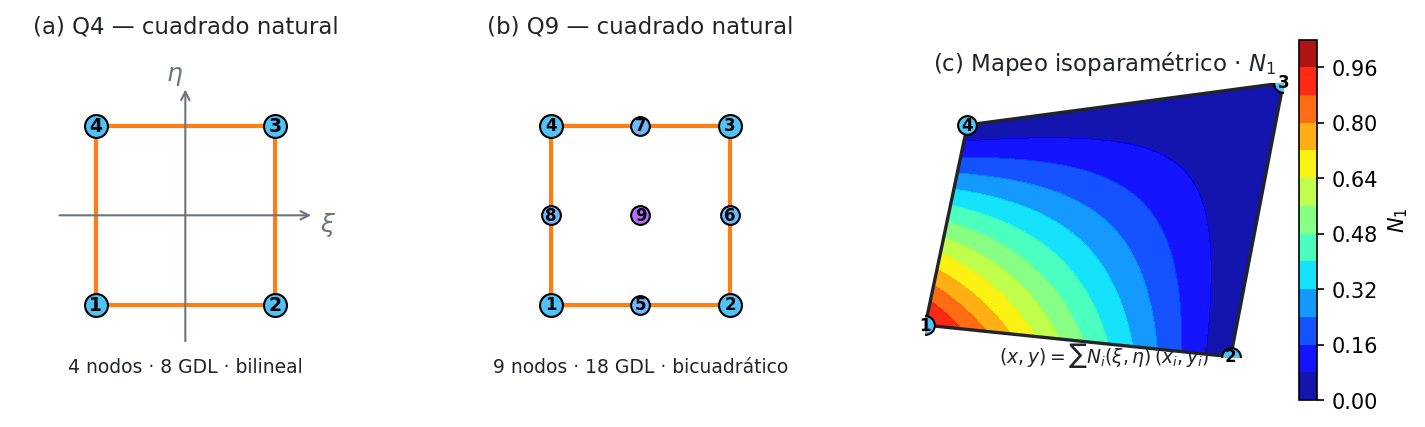
\includegraphics[width=\linewidth]{fig_isoparametricos}
\caption[Elementos isoparamétricos Q4 y Q9 y mapeo de un Q4 al espacio físico.]{Elementos isoparamétricos Q4 y Q9. En (a) y (b), el elemento de referencia de cada uno: un cuadrado de lado dos en coordenadas naturales $(\xi,\eta)$ entre $-1$ y $1$, con las esquinas numeradas en sentido antihorario desde la inferior izquierda; en el Q9 siguen los cuatro nodos medios, también en sentido antihorario, y el central. En (c), un elemento Q4 real de la malla, al que el mapeo isoparamétrico lleva cada punto del cuadrado; el color indica el valor de la función de forma $N_1$, que vale uno en el nodo~1 y cero en los otros tres. Esta numeración es la que emplean el motor de cálculo y la matriz de extrapolación de la \autoref{eq:extrap-q4}.}
\label{fig:isoparametricos}
\end{figure}

\section{Jacobiano del mapeo}
\label{sec:jacobiano}

El mapeo de la \autoref{eq:mapeo-iso} relaciona los dos espacios mediante la matriz Jacobiana, el cuadro de derivadas que registra cuánto se estira y se gira el elemento al pasar del cuadrado de referencia a su forma real, y que relaciona las derivadas respecto de las coordenadas naturales con las derivadas respecto de las físicas:

\begin{equation}
\bm{J} =
\begin{bmatrix}
\dfrac{\partial x}{\partial \xi} & \dfrac{\partial y}{\partial \xi} \\[6pt]
\dfrac{\partial x}{\partial \eta} & \dfrac{\partial y}{\partial \eta}
\end{bmatrix}
= \frac{\partial \bm{N}}{\partial(\xi,\eta)}\,\bm{X}_e,
\label{eq:jacobiano}
\end{equation}
donde $\partial\bm{N}/\partial(\xi,\eta)$ es la matriz $2\times n$ cuyas filas son las derivadas $\partial N_i/\partial\xi$ y $\partial N_i/\partial\eta$ (aquí $\bm{N}$ designa la fila de funciones de forma, no la matriz de interpolación de la \autoref{sec:formulacion-debil}), y $\bm{X}_e$ ($n\times 2$) reúne las coordenadas nodales del elemento. Esta es la convención de Bathe \autocite[p.~346]{bathe2014fem}, que es también la que implementa el motor. Con ella, cada fila de $\bm{J}$ es el vector tangente a una línea de coordenada natural ($\partial\bm{x}/\partial\xi$ y $\partial\bm{x}/\partial\eta$), y la regla de la cadena de la \autoref{eq:fisica-natural} emplea $\bm{J}^{-1}$ directamente. La convención transpuesta, también frecuente en la literatura, exigiría en su lugar $\bm{J}^{-T}$. El determinante del Jacobiano mide el factor local de cambio de área entre ambos espacios, $dx\,dy = \lvert\det\bm{J}\rvert\,d\xi\,d\eta$: es el número por el que hay que multiplicar un área del cuadrado de referencia para obtener la del elemento real, y por eso resulta central en la integración numérica. Para una matriz $2\times2$ se calcula explícitamente,

\begin{equation}
\det\bm{J} = J_{11}J_{22} - J_{12}J_{21},
\label{eq:detJ}
\end{equation}
y su inversa se obtiene por cofactores, evitando rutinas genéricas de inversión:

\begin{equation}
\bm{J}^{-1} = \frac{1}{\det\bm{J}}
\begin{bmatrix}
J_{22} & -J_{12} \\
-J_{21} & J_{11}
\end{bmatrix}.
\label{eq:invJ}
\end{equation}

Exigir $\det\bm{J} > 0$ en todo el elemento, con el determinante de la \autoref{eq:detJ}, garantiza por construcción que el mapeo sea biyectivo ---que a cada punto del cuadrado de referencia le corresponda uno solo del elemento, sin que este se pliegue sobre sí mismo--- y el elemento válido \autocites[pp.~346-347]{bathe2014fem}[p.~236]{cook2002concepts}. Un determinante nulo o negativo indica un elemento degenerado o invertido, y un programa de cálculo debe detectarlo antes de resolver. La condición y su comprobación son distintas: la condición se exige en todo el elemento, mientras que un programa la comprueba en un número finito de puntos, y el muestreo elegido determina qué defectos quedan a la vista. Los controles con que EduFEM lo resuelve se describen en la \autoref{sec:motor}.

\section{Matriz de deformación-desplazamiento \texorpdfstring{$\bm{B}$}{B}}
\label{sec:matriz-b}

Las deformaciones se obtienen derivando el campo de desplazamientos interpolado. La relación cinemática en elasticidad plana es

\begin{equation}
\bm{\varepsilon} =
\begin{bmatrix} \varepsilon_x \\ \varepsilon_y \\ \gamma_{xy} \end{bmatrix}
=
\begin{bmatrix}
\dfrac{\partial u}{\partial x} \\[4pt]
\dfrac{\partial v}{\partial y} \\[4pt]
\dfrac{\partial u}{\partial y} + \dfrac{\partial v}{\partial x}
\end{bmatrix},
\label{eq:cinematica}
\end{equation}
que en forma matricial se escribe $\bm{\varepsilon} = \bm{B}\,\bm{u}_e$, donde $\bm{u}_e$ reúne los desplazamientos de los nodos del elemento. La matriz $\bm{B}$, de dimensión $3 \times 2n$, es la que convierte esos desplazamientos nodales en deformaciones, y contiene para ello las derivadas físicas de las funciones de forma:

\begin{equation}
\bm{B} =
\begin{bmatrix}
\dfrac{\partial N_1}{\partial x} & 0 & \dfrac{\partial N_2}{\partial x} & 0 & \cdots \\[6pt]
0 & \dfrac{\partial N_1}{\partial y} & 0 & \dfrac{\partial N_2}{\partial y} & \cdots \\[6pt]
\dfrac{\partial N_1}{\partial y} & \dfrac{\partial N_1}{\partial x} & \dfrac{\partial N_2}{\partial y} & \dfrac{\partial N_2}{\partial x} & \cdots
\end{bmatrix}.
\label{eq:matriz-B}
\end{equation}

Las funciones de forma se definen en coordenadas naturales, pero $\bm{B}$ exige sus derivadas físicas $\partial N_i/\partial x$ y $\partial N_i/\partial y$. El puente lo provee la inversa del Jacobiano de la \autoref{eq:invJ}, aplicada por columna a cada función de forma según la regla de la cadena:

\begin{equation}
\begin{bmatrix}
\dfrac{\partial N_i}{\partial x} \\[6pt]
\dfrac{\partial N_i}{\partial y}
\end{bmatrix}
= \bm{J}^{-1}
\begin{bmatrix}
\dfrac{\partial N_i}{\partial \xi} \\[6pt]
\dfrac{\partial N_i}{\partial \eta}
\end{bmatrix}.
\label{eq:fisica-natural}
\end{equation}

Esta relación vectorial es la conexión esencial entre el espacio natural, donde las derivadas se conocen analíticamente, y el espacio físico, donde se formula la deformación.

\section{Matriz de rigidez elemental e integración numérica de Gauss}
\label{sec:rigidez-gauss}

La matriz de rigidez de un elemento liga las fuerzas en sus nodos con los desplazamientos de esos nodos, como la de una barra en un pórtico (\autoref{sec:formulacion-debil}). Reúne las tres piezas anteriores en un producto que se lee de derecha a izquierda: $\bm{B}$ convierte los desplazamientos nodales en deformaciones, $\bm{D}$ convierte esas deformaciones en tensiones y $\bm{B}^T$ devuelve las fuerzas nodales que las equilibran. Integrar ese producto sobre el dominio físico del elemento, con $t$ el espesor, suma la contribución de todos los puntos de su interior:

\begin{equation}
\bm{k}_e = \int_{\Omega_e} \bm{B}^T \bm{D}\, \bm{B}\, t \; dA
= \int_{-1}^{1}\!\!\int_{-1}^{1} \bm{B}^T(\xi,\eta)\,\bm{D}\,\bm{B}(\xi,\eta)\, t\, \lvert\det\bm{J}\rvert\; d\xi\, d\eta.
\label{eq:ke-integral}
\end{equation}

El integrando de la \autoref{eq:ke-integral} no es polinómico: como $\bm{B}$ depende de $\bm{J}^{-1}$, que es racional en $(\xi,\eta)$, la integración algebraica exacta deja de ser practicable salvo en los elementos más simples \autocites[p.~147]{zienkiewicz2013fem}[p.~191]{hughes2000fem}. Por ello se aproxima mediante cuadratura de Gauss-Legendre, que evalúa el integrando en puntos óptimos y lo pondera:

\begin{equation}
\bm{k}_e \approx \sum_{g=1}^{n_g} w_g\; \bm{B}^T(\xi_g,\eta_g)\,\bm{D}\,\bm{B}(\xi_g,\eta_g)\, t\, \lvert\det\bm{J}(\xi_g,\eta_g)\rvert,
\label{eq:ke-gauss}
\end{equation}
donde $g$ recorre los $n_g$ puntos de cuadratura del elemento, y los puntos $(\xi_g,\eta_g)$ y los pesos $w_g$ surgen del producto tensorial de la regla unidimensional. La regla de $m$ puntos integra exactamente polinomios de grado $2m-1$ \autocites[pp.~141-142]{hughes2000fem}[p.~161]{zienkiewicz2013fem}. La integración completa de esta familia es la cuadratura $2\times2$ para Q4 (cuatro puntos en $\xi = \pm 1/\sqrt{3}$) y $3\times3$ para Q9 (puntos en $\xi = \pm\sqrt{3/5},\,0$ con pesos $5/9,\,8/9,\,5/9$), órdenes que integran exactamente la rigidez de los respectivos elementos no distorsionados \autocites[pp.~221-222]{hughes2000fem}[p.~470]{bathe2014fem}; es la que adopta el motor. Esos puntos de Gauss no son nodos ni puntos que el usuario dibuja: son posiciones fijas del interior del elemento, y por eso reaparecen en la recuperación de tensiones (\autoref{sec:resolucion-tensiones}), en las métricas de calidad (\autoref{sec:calidad-malla}) y en la memoria de cálculo; la \autoref{fig:mod-m5} los muestra sobre un elemento real.

El orden de integración no es arbitrario. Una \emph{subintegración} puede dejar la matriz de rigidez con rango deficiente y admitir modos de deformación de energía nula, los modos espurios (\emph{hourglass}) que se analizan en la \autoref{sec:locking}. Una \emph{sobreintegración}, por ejemplo $3\times3$ en Q4, no aporta precisión apreciable y solo encarece el cálculo: el integrando solo es polinómico en los elementos no distorsionados, y en los distorsionados la diferencia es marginal, salvo distorsiones muy grandes, para las que se recomienda un orden mayor \autocite[p.~476]{bathe2014fem}. La elección de $2\times2$ para Q4 y $3\times3$ para Q9 equilibra exactitud y estabilidad para esta familia de elementos.

\section{Fenómenos numéricos en elementos de bajo orden: bloqueo y modos espurios}
\label{sec:locking}

La discretización con elementos de bajo orden introduce fenómenos numéricos que no provienen de la física del problema, sino de las limitaciones de la interpolación o de la integración numérica, y cuya comprensión resulta esencial para interpretar correctamente los resultados \autocite{cook2002concepts,hughes2000fem,bathe2014fem}. Tres son particularmente relevantes para los cuadriláteros que emplea EduFEM.

El \textbf{bloqueo por cortante} (\emph{shear locking}) afecta al elemento bilineal Q4 en estados dominados por flexión. Bajo flexión pura, una sección debería curvarse sin desarrollar deformación de corte; sin embargo, el campo de desplazamientos bilineal del Q4 no puede representar esa curvatura sin generar al mismo tiempo deformaciones de corte espurias, ausentes en la solución exacta. Esas deformaciones parásitas absorben energía y vuelven al elemento artificialmente rígido: por eso subestima los desplazamientos y converge con lentitud al refinar la malla \autocites[pp.~98-99]{cook2002concepts}[p.~243]{hughes2000fem}. El elemento Q9, cuya interpolación bicuadrática sí reproduce el modo de curvatura, está prácticamente libre de este bloqueo \autocites[pp.~235-236]{cook2002concepts}[p.~243]{hughes2000fem}. El \autoref{cap:resultados} lo cuantifica.

El \textbf{bloqueo volumétrico} (\emph{volumetric locking}) aparece en deformación plana cuando el material se aproxima a la incompresibilidad ($\nu \to 0{,}5$). Como anticipó la \autoref{sec:elasticidad-plana}, el factor $(1-2\nu)$ del denominador de $\bm{D}_{\text{DP}}$ tiende a cero, y la restricción de incompresibilidad sobrecondiciona el elemento: la malla no dispone de grados de libertad suficientes para satisfacer la condición $\varepsilon_x + \varepsilon_y \to 0$ en cada punto sin rigidizarse en exceso. El resultado es, de nuevo, una respuesta artificialmente rígida, acompañada a menudo de oscilaciones espurias en el campo de tensiones \autocites[pp.~192, 208]{hughes2000fem}[pp.~282-283]{bathe2014fem}.

Los \textbf{modos espurios} (\emph{hourglass}) son el fenómeno inverso: en lugar de rigidizar el elemento, lo ablandan. Como se anticipó en la \autoref{sec:rigidez-gauss}, surgen al \emph{subintegrar} la rigidez, por ejemplo evaluando el Q4 con un único punto de Gauss. La matriz elemental queda entonces con rango deficiente y admite modos de deformación de energía nula: formas de deformación que el elemento adopta sin oponer resistencia alguna, porque en el único punto donde se mide la deformación esta resulta nula, y que dibujan sobre la malla el patrón de reloj de arena que da nombre al fenómeno \autocites[pp.~223-224]{cook2002concepts}[pp.~472-473]{bathe2014fem}. Al no costar energía, esos patrones no físicos pueden crecer sin control y contaminar la solución. EduFEM los evita empleando la integración completa de cada elemento ($2\times2$ para Q4 y $3\times3$ para Q9).

Existen técnicas correctivas para los dos bloqueos. Una es la integración reducida selectiva (SRI), que integra con menos puntos de Gauss únicamente la parte de la rigidez responsable del bloqueo y deja el resto con la cuadratura completa \autocites[p.~221]{hughes2000fem}[pp.~476-477]{bathe2014fem}. Otra es la formulación $\bar{\bm{B}}$ (\emph{B-bar}), que promedia sobre el elemento esa misma parte del operador de deformación en lugar de evaluarla punto por punto \autocite[pp.~232-234]{hughes2000fem}. EduFEM no las implementa: ofrece en su lugar el elemento Q9, que evita el bloqueo por cortante por la vía del mayor orden de interpolación, aunque no el volumétrico, frente al cual el bicuadrático con integración completa también requiere integración selectiva \autocite[p.~222]{hughes2000fem}. Además, conserva el comportamiento del Q4 sin corregirlo, para que el bloqueo quede visible en los resultados que el software presenta en lugar de quedar compensado dentro del cálculo. La incorporación de esas técnicas correctivas se plantea como línea de extensión futura entre las recomendaciones del trabajo.

\section{Ensamblaje, restricciones y cargas}
\label{sec:ensamblaje}

Las matrices elementales de la \autoref{eq:ke-gauss} y los vectores de carga de cada elemento se ensamblan en el sistema global mediante el mapeo de cada GDL local a su índice global. La matriz de rigidez global se obtiene con el operador de ensamblaje, que aquí se denota $\Ensamblaje$ y que no es otra cosa que la suma de cada aporte elemental en las filas y columnas que le corresponden según ese mapeo:

\begin{equation}
\bm{K} = \Ensamblaje_{e} \bm{k}_e, \qquad
\bm{F} = \Ensamblaje_{e} \bm{f}_e^{\text{vol}} + \sum_j \bm{F}_j + \sum_\Gamma \bm{F}_\Gamma,
\label{eq:ensamblaje}
\end{equation}
donde $e$ recorre los elementos de la malla, $j$ los nodos cargados y $\Gamma$ las aristas con carga de superficie, y donde un nodo compartido por varios elementos acumula los aportes de todos ellos. Para mallas grandes $\bm{K}$ es dispersa (mayoritariamente nula), por lo que EduFEM la construye en formato de coordenadas (COO) y la convierte a filas comprimidas (CSR) para el solucionador, apoyándose en el módulo de matrices dispersas de SciPy \autocite[p.~265]{virtanen2020scipy}.

El vector de cargas reúne tres aportes. Las \textbf{cargas nodales} $\bm{F}_j$ se aplican directamente en los GDL del nodo $j$. Las \textbf{cargas volumétricas} $\bm{f}_e^{\text{vol}}$, como la gravedad, se distribuyen consistentemente integrando $\int_{\Omega_e} \bm{N}^T \bm{b}\, t\, dA$ por cuadratura de Gauss. Las \textbf{cargas superficiales} $\bm{F}_\Gamma$ sobre una arista se convierten en fuerzas nodales equivalentes ponderando la carga distribuida con las funciones de forma. Para una arista lineal de Q4 de longitud $L$ con carga $q$ que varía linealmente entre los valores $q_1$ y $q_2$ de sus extremos, el reparto exacto es $F_1 = \tfrac{L}{6}(2q_1 + q_2)$ y $F_2 = \tfrac{L}{6}(q_1 + 2q_2)$, que con $q$ constante se reduce a $qL/2$ en cada nodo. Para la arista cuadrática de Q9 con $q$ constante la distribución resulta $\tfrac{qL}{6},\,\tfrac{4qL}{6},\,\tfrac{qL}{6}$, concentrando la mayor parte en el nodo medio \autocite[p.~113]{cook2002concepts}.

Las restricciones de Dirichlet se imponen partiendo el sistema en GDL libres ($f$) y restringidos ($r$):

\begin{equation}
\begin{bmatrix} \bm{K}_{ff} & \bm{K}_{fr} \\ \bm{K}_{rf} & \bm{K}_{rr} \end{bmatrix}
\begin{bmatrix} \bm{u}_f \\ \bm{u}_r \end{bmatrix}
=
\begin{bmatrix} \bm{F}_f \\ \bm{F}_r \end{bmatrix}.
\label{eq:particion}
\end{equation}

Para \emph{restricciones homogéneas} ($\bm{u}_r = \bm{0}$) basta resolver el bloque libre de la \autoref{eq:particion}, $\bm{K}_{ff}\,\bm{u}_f = \bm{F}_f$. Para \emph{restricciones no homogéneas} ($\bm{u}_r \neq \bm{0}$), necesarias en la verificación con soluciones manufacturadas, el sistema reducido lleva al segundo miembro el aporte de los desplazamientos impuestos

\begin{equation}
\bm{K}_{ff}\,\bm{u}_f = \bm{F}_f - \bm{K}_{fr}\,\bm{u}_r,
\label{eq:dirichlet-no-homogeneo}
\end{equation}
que preserva la simetría del bloque libre. Un modelo bien restringido hace que $\bm{K}_{ff}$ sea definida positiva, es decir, que todo desplazamiento no nulo de los GDL libres deforme el sólido y almacene energía, condición que asegura que la matriz no sea singular y, por tanto, que la solución sea única \autocite[pp.~726-727]{bathe2014fem}. Bien restringido significa aquí al menos tres GDL restringidos, dispuestos de modo que impidan las dos traslaciones y la rotación del sólido como cuerpo rígido: tres apoyos paralelos o tres apoyos concurrentes no bastan, igual que no bastan en el análisis de un pórtico.

\section{Resolución del sistema y recuperación de tensiones}
\label{sec:resolucion-tensiones}

El sistema reducido de la \autoref{eq:dirichlet-no-homogeneo} se resuelve por factorización directa sobre la matriz dispersa; el motor concreto y su reordenamiento se documentan en la \autoref{sec:motor}. Como $\bm{K}_{ff}$ es simétrica y definida positiva, admite además una factorización de Cholesky, $\bm{K}_{ff} = \bm{L}\bm{L}^{T}$, que almacena un solo triángulo y no requiere pivoteo; el motor emplea una factorización LU general, y la de Cholesky se reserva como línea de trabajo (\emph{Recomendaciones}). Conocido el vector $\bm{u}$, las reacciones en los GDL restringidos se recuperan como $\bm{R} = \bm{K}_{rf}\,\bm{u}_f + \bm{K}_{rr}\,\bm{u}_r - \bm{F}_r$.

Las tensiones se calculan primero en los puntos de Gauss, evaluando $\bm{\sigma}_g = \bm{D}\,\bm{B}_g\,\bm{u}_e$ en cada punto $g$. A partir de las componentes cartesianas se obtienen las tensiones principales \autocite[pp.~12-14]{timoshenko1970elasticity} y la equivalente de von Mises, la medida escalar con que habitualmente se resume el estado tensional completo \autocite[p.~117]{cook2002concepts}:

\begin{equation}
\begin{aligned}
\sigma_{1,2} &= \frac{\sigma_x + \sigma_y}{2} \pm \sqrt{\left(\frac{\sigma_x - \sigma_y}{2}\right)^2 + \tau_{xy}^2}, \\
\sigma_{\mathrm{VM}} &= \sqrt{\tfrac{1}{2}\left[(\sigma_1-\sigma_2)^2 + (\sigma_2-\sigma_z)^2 + (\sigma_z-\sigma_1)^2\right]}, \\
\sigma_z &=
\begin{cases}
0 & \text{tensión plana,}\\
\nu\,(\sigma_x+\sigma_y) & \text{deformación plana.}
\end{cases}
\end{aligned}
\label{eq:principales-vm}
\end{equation}

En tensión plana $\sigma_z = 0$ y la \autoref{eq:principales-vm} se reduce a la forma plana $\sigma_{\mathrm{VM}} = \sqrt{\sigma_1^2 - \sigma_1\sigma_2 + \sigma_2^2}$. En deformación plana la tensión fuera del plano no es nula y es la tercera tensión principal. Omitirla, simplificación a la que invita el carácter bidimensional del planteo, altera la tensión equivalente y puede sobreestimarla: con $\sigma_x = \sigma_y = 100$, $\tau_{xy} = 0$ y $\nu = 0{,}30$, el valor correcto es $40$ y el que resulta de imponer $\sigma_z = 0$ es $100$. Por eso EduFEM la incorpora en todas las rutas de cálculo del software, desde las tensiones en los puntos de Gauss hasta la consulta puntual sobre el modelo y la memoria de cálculo, con el $\nu$ del material de cada elemento.

Las tensiones no son igualmente exactas en todo el elemento: existen puntos de muestreo en los que convergen con un orden superior al del resto, propiedad que se conoce como superconvergencia y que en los elementos de esta familia corresponde a los puntos de Gauss de una regla de orden inferior al de la integración completa. En el Q9 son los cuatro puntos de la regla $2\times2$, y no los nueve de la regla $3\times3$ con que se integra su rigidez \autocite[pp.~230-231]{cook2002concepts}. EduFEM evalúa las tensiones en los puntos de la cuadratura de rigidez de cada elemento y las lleva a los nodos mediante una extrapolación, es decir, prolongando hasta ellos los valores medidos en el interior, con una matriz precalculada: $\bm{\sigma}_{\text{nodos}} = \bm{E}\,\bm{\sigma}_{\text{Gauss}}$, en lugar de evaluar $\bm{B}$ directamente en los nodos. Como recoge la Nomenclatura, $\bm{E}$, en negrita, designa la matriz de extrapolación y no el módulo de elasticidad $E$ de la \autoref{eq:D-tension-plana}, que se escribe sin negrita. Para el Q4 esa elección muestrea en los cuatro puntos de la regla $2\times2$, aunque Cook sitúa el punto superconvergente del elemento bilineal en su centro \autocite[p.~230]{cook2002concepts}: es una decisión de implementación que conserva la variación del campo dentro del elemento. Para el Q9 privilegia que la matriz $\bm{M}$ definida a continuación sea cuadrada con los nueve nodos del elemento, a costa de no muestrear en los puntos óptimos.

El costo esperable de esa decisión es doble: las tensiones nodales no heredan la precisión superior de los puntos óptimos, y la extrapolación amplifica las diferencias entre puntos de Gauss, pues los pesos de la matriz del Q4 llegan a $1{,}866$ y $-0{,}5$, como se ve más abajo en la \autoref{eq:extrap-q4}. A cambio, una única ruta de cálculo sirve a los dos tipos de elemento y conserva la variación del campo dentro de cada uno. El orden de convergencia que resulta de esta secuencia de muestreo, extrapolación y promediado no se toma de la literatura: se mide en el \autoref{cap:resultados} con el método de las soluciones manufacturadas.

La matriz de extrapolación $\bm{E}$ se deduce de la propia interpolación isoparamétrica. Dentro del elemento, el campo de tensiones se aproxima con las mismas funciones de forma que la geometría, las de la \autoref{eq:N-q4} y la \autoref{eq:N-q9}, de modo que el valor en un punto de Gauss es la interpolación de los valores nodales,

\begin{equation}
\bm{\sigma}(\xi_g,\eta_g) = \sum_{i=1}^{n} N_i(\xi_g,\eta_g)\,\bm{\sigma}_{\text{nodo},i}.
\label{eq:interp-tension}
\end{equation}

Evaluando la \autoref{eq:interp-tension} en los puntos de Gauss del elemento se obtiene el sistema $\bm{\sigma}_{\text{Gauss}} = \bm{M}\,\bm{\sigma}_{\text{nodos}}$, donde $M_{gi} = N_i(\xi_g,\eta_g)$ reúne las funciones de forma del nodo $i$ evaluadas en cada punto de Gauss $g$. Cuando el número de puntos de Gauss iguala al de nodos del elemento —cuadratura $2\times2$ para Q4 y $3\times3$ para Q9—, la matriz $\bm{M}$ es cuadrada e invertible, y la extrapolación es su inversa,

\begin{equation}
\bm{\sigma}_{\text{nodos}} = \bm{M}^{-1}\,\bm{\sigma}_{\text{Gauss}} = \bm{E}\,\bm{\sigma}_{\text{Gauss}}.
\label{eq:extrap-inversa}
\end{equation}

Para el elemento Q4 esta inversa admite forma cerrada. Como los cuatro puntos de Gauss se ubican en $(\pm 1/\sqrt{3},\,\pm 1/\sqrt{3})$ y los nodos en $(\pm 1,\,\pm 1)$, extrapolar equivale a evaluar la interpolación bilineal en coordenadas escaladas por $\sqrt{3}$, con entradas de la forma $\tfrac{1}{4}(1\pm\sqrt{3})(1\pm\sqrt{3})$. Con los puntos de Gauss numerados en el orden que produce el motor —$(-,-)$, $(-,+)$, $(+,-)$, $(+,+)$ en $(\xi,\eta)$— y los nodos en sentido antihorario desde $(-1,-1)$, resulta

\begin{equation}
\bm{E}_{\text{Q4}} =
\begin{bmatrix}
a & b & b & c \\
b & c & a & b \\
c & b & b & a \\
b & a & c & b
\end{bmatrix},
\qquad
a = 1+\frac{\sqrt{3}}{2},\quad
b = -\frac{1}{2},\quad
c = 1-\frac{\sqrt{3}}{2},
\label{eq:extrap-q4}
\end{equation}
con $a \approx 1{,}866$ y $c \approx 0{,}134$: cada nodo recibe el peso $a$ del punto de Gauss más próximo, $c$ del diagonalmente opuesto y $b$ de los otros dos. La numeración no es un detalle menor: permutar los puntos de Gauss permuta las columnas de $\bm{E}$, y una matriz escrita para otra numeración corrompe las tensiones nodales sin alterar los desplazamientos. Una verificación basada solo en desplazamientos no lo detecta. Por eso el motor construye $\bm{E}$ invirtiendo numéricamente $\bm{M}$ con sus propios puntos de Gauss, para Q4 igual que para Q9. Una prueba de regresión comprueba que $\bm{E}$ reproduce los campos bilineales (o bicuadráticos) de prueba con un error del orden de la precisión de máquina, que es la verificación numérica de la identidad algebraica de la que $\bm{E}$ se deduce. Para el Q9, $\bm{M}$ es de $9\times9$; su inversa también tiene forma cerrada, el producto tensorial de la extrapolación unidimensional por los tres puntos de Gauss, pero sus 81 entradas no se transcriben aquí. La extrapolación se aplica a las componentes cartesianas $(\sigma_x,\sigma_y,\tau_{xy})$; las tensiones principales y la de von Mises, al ser funciones no lineales de ellas, se recalculan a partir de las componentes ya extrapoladas en lugar de extrapolarse directamente: es el criterio que adopta EduFEM para que cada valor nodal sea consistente con sus propias componentes cartesianas.

Finalmente, como un nodo compartido recibe valores distintos desde cada elemento adyacente, se aplica un \emph{promediado nodal}

\begin{equation}
\bm{\sigma}_{\text{nodo}} = \frac{1}{n_e}\sum_{e=1}^{n_e} \bm{\sigma}_{\text{nodo}}^{(e)},
\label{eq:promediado}
\end{equation}
que suaviza el campo y produce un contorno continuo. El salto entre los valores sin promediar es, además, un indicador útil del error de discretización —es el principio en que se apoyan los estimadores de error por recuperación \autocite[pp.~476-477]{zienkiewicz2013fem}—: cuanto mayor es la dispersión entre elementos, mayor es el error de discretización en esa zona y más conviene refinar allí la malla.

\section{Calidad de malla}
\label{sec:calidad-malla}

La precisión del resultado depende de la calidad geométrica de los elementos. EduFEM evalúa dos métricas complementarias, tomadas de la biblioteca de calidad geométrica Verdict \autocite[p.~3]{stimpson2007verdict}, que miden propiedades distintas: una los ángulos del elemento y otra sus proporciones. Un rectángulo muy alargado, por ejemplo, tiene ángulos rectos impecables y proporciones inadmisibles. El \textbf{Jacobiano escalado} mide la distorsión angular normalizando el determinante del Jacobiano por las normas de sus filas, que son los vectores tangentes a las líneas $\xi$ y $\eta$,

\begin{equation}
q_{SJ} = \min_g \frac{\det\bm{J}_g}{\|\bm{J}_{1,:}\|_g\,\|\bm{J}_{2,:}\|_g},
\label{eq:scaled-jacobian}
\end{equation}
cantidad que equivale al seno del ángulo local entre ambas tangentes y vive en el rango $[-1, 1]$: vale $1$ cuando las dos tangentes son perpendiculares, indica baja calidad cerca de $0$ y delata un elemento degenerado o invertido cuando $q_{SJ} \le 0$ \autocite[pp.~36, 51]{stimpson2007verdict}. La memoria de cálculo la evalúa en los puntos de Gauss del elemento. El módulo introductorio de calidad de malla (\autoref{sec:educacion}) emplea la forma por vértices de Verdict: el seno del ángulo interior en cada esquina, tomando el peor de los cuatro. El módulo marca ese peor ángulo sobre el lienzo y muestra el valor de la métrica en una barra, de modo que el número puede comprobarse a mano con el seno de ese ángulo. La \textbf{compacidad} o \emph{stretch} mide la proporción del elemento relacionando su arista más corta $L_{\min}$ con su diagonal más larga $D_{\max}$,

\begin{equation}
q_C = \sqrt{2}\,\frac{L_{\min}}{D_{\max}} \in [0, 1],
\label{eq:stretch}
\end{equation}
que vale $1$ para un cuadrado perfecto y disminuye al alargarse o aplastarse el elemento \autocite[p.~57]{stimpson2007verdict}. El subíndice $C$ recuerda que se trata de la compacidad, y evita confundir el símbolo con los nombres Q4 y Q9 de los elementos. De la documentación de Verdict provienen los mínimos admisibles del cuadrilátero, $q_{SJ} \ge 0{,}30$ y $q_C \ge 0{,}25$ \autocite[pp.~51, 57]{stimpson2007verdict}; los cortes con que el software clasifica los elementos, entre ellos el mínimo de $q_{SJ}$ que el módulo M0 eleva a $0{,}50$, son decisiones de implementación, documentadas en la \autoref{sec:pre-proceso}.

Esas dos métricas son las que presenta el módulo introductorio de calidad de malla. El estado global de calidad que la memoria de cálculo asigna a cada elemento —buena, aceptable o mala— se apoya, en cambio, en cuatro métricas, porque un elemento puede fallar de cuatro maneras y cada métrica vigila una:

\begin{itemize}
    \item los ángulos, con el Jacobiano escalado $q_{SJ}$;
    \item la uniformidad del mapeo de un extremo al otro del elemento, con la razón de Jacobianos $R_J$;
    \item el alargamiento, con la relación de aspecto $AR$;
    \item la trapecialidad, con el estrechamiento $T_R$.
\end{itemize}

Las dos primeras métricas salen del propio Jacobiano: el $q_{SJ}$ de la \autoref{eq:scaled-jacobian}, evaluado en los puntos de Gauss, y la razón $R_J = \min_g \det\bm{J}_g / \max_g \det\bm{J}_g$ entre el menor y el mayor de sus determinantes. Las dos restantes se construyen sobre una descomposición bilineal del cuadrilátero, equivalente a la que Verdict emplea para sus métricas de forma \autocite[pp.~35-36]{stimpson2007verdict}. La descomposición reduce las coordenadas de las cuatro esquinas $\bm{r}_1,\dots,\bm{r}_4$ a tres vectores característicos. Los dos primeros son la mitad de los vectores que unen los puntos medios de las aristas opuestas en cada dirección natural y miden la extensión del elemento; el tercero recoge su parte propiamente bilineal. De ellos se derivan la \textbf{relación de aspecto} $AR$ y el \textbf{estrechamiento} (\emph{taper}) $T_R$:

\begin{equation}
\begin{aligned}
\bm{X}_1 &= \tfrac{1}{4}\left(-\bm{r}_1 + \bm{r}_2 + \bm{r}_3 - \bm{r}_4\right), \qquad
\bm{X}_2 = \tfrac{1}{4}\left(-\bm{r}_1 - \bm{r}_2 + \bm{r}_3 + \bm{r}_4\right), \\[2pt]
\bm{X}_3 &= \tfrac{1}{4}\left(\bm{r}_1 - \bm{r}_2 + \bm{r}_3 - \bm{r}_4\right), \\[4pt]
AR &= \frac{\max(\|\bm{X}_1\|, \|\bm{X}_2\|)}{\min(\|\bm{X}_1\|, \|\bm{X}_2\|)}, \qquad
T_R = \max\left(\frac{|\bm{X}_3 \cdot \bm{X}_1|}{\|\bm{X}_1\|^2},\; \frac{|\bm{X}_3 \cdot \bm{X}_2|}{\|\bm{X}_2\|^2}\right).
\end{aligned}
\label{eq:descomposicion-bilineal}
\end{equation}

La relación de aspecto vale $1$ en un cuadrado o un rombo y crece al alargarse el elemento. El estrechamiento es nulo en todo paralelogramo y crece con la trapecialidad: precisamente el modo de distorsión ante el que el Q4 es más sensible, como muestra el caso de Cook del \autoref{cap:resultados}. En el Q9 la cuarta métrica no es el estrechamiento, sino la desviación de los nodos de arista y central respecto de su posición ideal: el punto medio de la arista recta entre esquinas, para cada nodo de arista, y el promedio de los cuatro nodos de arista, para el central. Los cortes con que se asigna el estado global no son umbrales bibliográficos sino convención del software, y se enumeran en la \autoref{sec:pre-proceso}; la \autoref{fig:mod-m0} muestra el Jacobiano escalado y la compacidad evaluados sobre una malla.

\section{Verificación y validación}
\label{sec:verificacion-validacion}

Un programa de cálculo debe distinguir entre \emph{verificación}, que comprueba que las ecuaciones se resuelven correctamente, y \emph{validación}, que comprueba que las ecuaciones representan la realidad física \autocite[pp.~13-14]{oberkampf2010vv}. Este trabajo aplica ambas estrategias, y en todo el documento entiende la verificación en sentido estricto y la validación como contraste con referencias externas de exactitud conocida, no como campaña experimental. En su acepción estricta, en efecto, la validación exige el contraste con mediciones experimentales, y este trabajo no realiza campaña experimental propia. Sus referencias externas de exactitud conocida son una solución analítica de la teoría de la elasticidad y el valor de referencia de uso extendido de la membrana de Cook; a ellas se suma un modelo equivalente resuelto en un programa comercial, que sirve de comparación y no es patrón de exactitud (\autoref{sec:timoshenko}). El contraste corresponde, por tanto, a verificación de solución ---estimar el error numérico de una solución concreta, y no comprobar el código en general--- y a comparación código a código. Esta última, según la propia literatura, no sustituye a la verificación rigurosa del código \autocite[pp.~173-174]{oberkampf2010vv}.

El documento emplea además «cobertura de contenido» para el contraste documental del \autoref{cap:resultados}, que no es validación en el sentido de esta sección, y «comprobador de salud» para la revisión automática de los datos de entrada, que es el nombre de un componente del software. En el tercer objetivo específico, por último, «verificar y validar EduFEM», el verbo \emph{validar} cubre dos sentidos: el de esta sección, para la exactitud del motor frente a referencias externas, y el metodológico corriente ---comprobar que la solución construida satisface sus criterios de aceptación explícitos---, para la cobertura del procedimiento y del contenido. La sigla V\&V, de uso habitual en la disciplina, abrevia «verificación y validación» en ese doble sentido.

La verificación de código se realiza con el \textbf{Método de las Soluciones Manufacturadas} (MMS): se elige a priori un campo de desplazamientos exacto $\bm{u}_M$ y se sustituye en las ecuaciones de equilibrio para deducir la fuerza de cuerpo $\bm{b} = -\nabla\cdot\bm{\sigma}(\bm{u}_M)$ que lo produce. Después se inyectan esa carga y las restricciones de Dirichlet no homogéneas correspondientes, es decir, desplazamientos impuestos distintos de cero en el contorno \autocites[pp.~21, 26]{salari2000mms}[pp.~219-222]{oberkampf2010vv}.

Para comparar la solución de EduFEM con la exacta no basta mirar un punto: hace falta una medida única del error en toda la pieza. La norma $L^2$ del desplazamiento es esa medida: la raíz cuadrada de la integral, extendida a toda la pieza, del cuadrado de la diferencia entre el desplazamiento calculado y el exacto, que resume en un solo número el desajuste en todo el dominio. La seminorma $H^1$ hace lo mismo con los gradientes del desplazamiento, de los que se obtienen las deformaciones, que son las que determinan las tensiones que el ingeniero acaba leyendo; por eso converge más despacio y es la medida más exigente de las dos. Al reducir a la mitad el tamaño $h$ de los elementos, ambas medidas deben caer en una proporción fija que la teoría predice. El exponente de esa caída, es decir, la potencia de $h$ a la que resulta proporcional el error, es la \emph{tasa de convergencia}. La proporción depende del \emph{orden} $p$ del elemento, que es el grado del polinomio completo que contiene su interpolación: $p = 1$ para el Q4 bilineal y $p = 2$ para el Q9 bicuadrático. El orden fija cuánto cuesta ganar exactitud: con tasa $2$, esa reducción a la mitad divide el error por cuatro; con tasa $3$, por ocho.

Con esa lectura, el error de la solución numérica frente a la exacta se cuantifica con la norma $L^2$ del desplazamiento y la seminorma $H^1$:

\begin{equation}
\begin{aligned}
\|\bm{u}_h - \bm{u}\|_{L^2} &= \left( \int_\Omega \|\bm{u}_h - \bm{u}\|^2 \, d\Omega \right)^{1/2}, \\
|\bm{u}_h - \bm{u}|_{H^1} &= \left( \int_\Omega \|\nabla\bm{u}_h - \nabla\bm{u}\|^2 \, d\Omega \right)^{1/2}.
\end{aligned}
\label{eq:normas-error}
\end{equation}

En la \autoref{eq:normas-error}, $\bm{u}$ es la solución exacta manufacturada y $\bm{u}_h$ la calculada sobre una malla de tamaño característico $h$. En los miembros izquierdos, las barras dobles denotan la norma $L^2$ y las simples la seminorma $H^1$; dentro de las integrales, $\|\cdot\|$ es, en cada punto, la raíz de la suma de los cuadrados de las componentes del vector de desplazamiento o de su gradiente. Más abajo aparece además $\bm{\sigma}^*_h$, donde el asterisco distingue el campo de tensiones recuperado, extrapolado a los nodos y promediado, del evaluado directamente en los puntos de Gauss.

Al refinar la malla, estas medidas deben decrecer con las tasas asintóticas teóricas ($\mathcal{O}(h^{p+1})$ en $L^2$ y $\mathcal{O}(h^p)$ en la seminorma $H^1$, con $p$ el orden polinómico del elemento) que establece la teoría de aproximación del MEF \autocites[pp.~106-107]{strang2008analysis}[pp.~189-190]{hughes2000fem}. En un problema de solución suave, como el de las soluciones manufacturadas, una tasa observada inferior a la teórica delata un defecto de implementación; alcanzarla es la evidencia más exigente de que las rutinas ejercitadas por esa medida están correctamente implementadas en los términos a los que la solución elegida es sensible. Alcanzarla no descarta, sin embargo, errores en las rutas que la medida no recorre ni en los términos que esa solución anula (\autoref{sec:mms}).

Las integrales de error se evalúan con un punto de Gauss más por dirección que la rigidez, es decir, $3\times3$ para Q4 y $4\times4$ para Q9, para no subestimar artificialmente el error. Es una precaución de implementación de los propios guiones de verificación ---los programas de Python que arman cada caso, lo resuelven y calculan sus errores---. El integrando de la norma es el cuadrado de una diferencia entre dos campos, de grado más alto que el integrando de la rigidez, y una cuadratura ajustada a esta última lo integra con menos exactitud: el error de esa cuadratura se confundiría con el que se quiere medir.

Como esas medidas dependen solo del campo de desplazamientos, no ejercitan la secuencia de recuperación de tensiones, esto es, la evaluación en los puntos de Gauss, la extrapolación a los nodos y el promediado. Por ello se mide además la norma $L^2$ del campo de tensiones recuperado $\bm{\sigma}^*_h$ frente a $\bm{\sigma}(\bm{u}_M)=\bm{D}\,\bm{\varepsilon}(\bm{u}_M)$, porque el error de las magnitudes derivadas debe verificarse por separado y su orden puede ser menor que el de la solución primaria \autocite[p.~29]{salari2000mms}. La matriz de extrapolación tiene su propia prueba de reproducción de campos polinómicos, descrita en la \autoref{sec:resolucion-tensiones}.

La validación, en la acepción fijada arriba, contrasta el motor con casos de estudio de solución conocida. La \textbf{viga de Timoshenko} simplemente apoyada admite solución analítica de la teoría de la elasticidad \autocite[art.~21, pp.~39-43]{timoshenko1970elasticity}; el \autoref{cap:resultados} contrasta con ella la tensión normal y la flecha, y las compara además con un modelo de cáscara de SAP2000 \autocite[p.~179]{csi2017sap2000}. La \textbf{membrana de Cook} es el caso clásico con que la literatura evidencia la sensibilidad de los elementos a la distorsión geométrica y al bloqueo por cortante. En ella el elemento Q4 subestima sensiblemente el desplazamiento del extremo en las mallas gruesas, por el bloqueo descrito en la \autoref{sec:locking} \autocite[pp.~98-99]{cook2002concepts}, mientras que el Q9, de orden superior, lo evita y converge con rapidez \autocite[p.~243]{hughes2000fem}. El valor de uso extendido para ese desplazamiento, $23{,}96$, se corrobora en este trabajo con una extrapolación de Richardson propia, es decir, con el procedimiento que estima el valor exacto desconocido a partir de tres mallas sucesivas; la \autoref{sec:cook} presenta el caso completo, con su geometría, su valor de referencia y esa corroboración. Estos contrastes muestran por qué la elección del tipo de elemento condiciona la calidad del resultado.

Con lo expuesto en este capítulo queda establecida la base común del motor de cálculo, de los módulos educativos y de la memoria de cálculo. Una misma formulación, las mismas matrices y los mismos criterios de verificación y validación sirven a los tres. Lo que el motor calcula, lo que los módulos muestran sobre el modelo y lo que la memoria escribe paso a paso son, así, el mismo procedimiento leído con distinto detalle. Con ello, junto con los antecedentes y los requisitos de la \autoref{sec:antecedentes}, se cumple el primer objetivo específico. El \autoref{cap:diseno} traduce esta base en decisiones de diseño y de implementación.

\chapter{Desarrollo de EduFEM en Python ---motor de cálculo, interfaz, módulos educativos y memoria de cálculo--- para exponer el procedimiento de cálculo etapa por etapa sobre el modelo del usuario}
\label{cap:diseno}
\chaptermark{Desarrollo de EduFEM}% nombre corto para el pie de página

Este capítulo cumple el segundo objetivo específico: el desarrollo de EduFEM. Fija primero el diseño metodológico con que el software se construye y se evalúa (\autoref{sec:metodologia}) y describe después el software que lo concreta (\autoref{sec:diseno-edufem}). La palabra \emph{modelo} tiene aquí dos acepciones distintas. En el diseño metodológico designa el modelo de la investigación: sus variables, sus casos de estudio y sus instrumentos. En la descripción del software designa el modelo numérico de elementos finitos que EduFEM implementa. El primero antecede y encuadra al segundo.

\section{Diseño metodológico}
\label{sec:metodologia}

Esta sección sigue la estructura de un modelo de investigación: la conceptualización y el alcance, la definición de las variables, el procedimiento y la toma de observaciones, la confiabilidad de esas observaciones y el contraste de la hipótesis con los resultados.

\subsection{Tipo de investigación, método y modelo de simulación numérica}
\label{sec:proceso-met}

El trabajo se clasifica según cuatro criterios: finalidad, naturaleza, enfoque y nivel. Por su finalidad es \emph{propositivo}: propone una solución a un problema concreto. Por su naturaleza es una \emph{investigación tecnológica}, la que busca conocimiento de carácter operativo y no solo establece cuál es la solución, sino que brinda la información para llevarla a cabo \autocite[p.~91]{garciacordoba2005tecnologica}. Por el abordaje del problema, el enfoque es \emph{cuantitativo} \autocite[p.~6]{sampieri2018metodologia}: la exactitud del software se establece midiendo errores numéricos, tensiones, desplazamientos y tasas de convergencia, y la exposición del procedimiento se establece contando qué etapas y qué contenidos quedan a la vista. La recolección de datos combina la medición numérica sobre el motor con el inventario documentado de lo que el software expone. Por su nivel es \emph{descriptivo} y \emph{comparativo}: caracteriza el comportamiento numérico del motor y lo compara con referencias externas, contrasta el desempeño de los elementos Q4 y Q9, y sitúa el software frente a los recursos existentes.

\paragraph{Método} El método es el de la \emph{ciencia del diseño}. En ella, el conocimiento sobre un problema y su solución se obtiene construyendo un producto tecnológico —el \emph{artefacto}, en la terminología del método; aquí, EduFEM— y evaluándolo con rigor \autocite[pp.~75, 83]{hevner2004design}. Lo que distingue una investigación de este tipo de un diseño rutinario es que deja una contribución identificable a la base de conocimiento, y no solo un producto \autocite[p.~81]{hevner2004design}; las contribuciones de este trabajo se recogen en las Conclusiones. El proceso tiene seis actividades \autocite[pp.~52-56]{peffers2007dsrm}, que la \autoref{tab:dsrm} ubica en este documento.

\begin{table}[htbp]
\centering
\caption[Las seis actividades del método de la ciencia del diseño en este trabajo.]{Las seis actividades del método de la ciencia del diseño \autocite[pp.~52-56]{peffers2007dsrm} y la base de conocimiento sobre la que se apoyan: qué es cada una en este trabajo, dónde se desarrolla y a qué objetivo específico (OE) responde. La tabla registra la aplicación del método de diseño que nombra la hipótesis. La fila «Base de conocimiento» no es una actividad del proceso, sino el fondo teórico del que las actividades 2 y 3 toman sus insumos.}
\label{tab:dsrm}
{\footnotesize
\setlength{\tabcolsep}{3pt}
\renewcommand{\arraystretch}{1.15}
\begin{tabular}{@{}>{\raggedright\arraybackslash}p{3.3cm}>{\raggedright\arraybackslash}p{6.4cm}>{\raggedright\arraybackslash}p{3.0cm}>{\raggedright\arraybackslash}p{1.2cm}@{}}
\toprule
\textbf{Actividad} & \textbf{En este trabajo} & \textbf{Dónde} & \textbf{OE} \\
\midrule
1. Identificar el problema y motivar & El software usado como caja negra deja un análisis que no puede seguirse ni comprobarse & Introducción; \autoref{sec:antecedentes} & --- \\
2. Definir los objetivos de la solución & Requisitos: procedimiento completo a la vista, memoria reproducible a mano, exactitud dentro de tolerancias explícitas, contenido exigido por los expertos, software libre y en español & \autoref{sec:antecedentes}; \autoref{sec:requisitos}; \autoref{sec:validacion-resultados} & 1 \\
\midrule
Base de conocimiento & El MEF en elasticidad plana, la verificación y validación, y los principios que orientan la exposición & \autoref{cap:marco_teorico} & 1 \\
\midrule
3. Diseñar y desarrollar & Motor de cálculo, interfaz, módulos educativos y memoria de cálculo & \autoref{sec:diseno-edufem} & 2 \\
4. Demostrar & Resolver instancias del problema: el ejemplo guía paso a paso y los tres casos de estudio & \autoref{sec:mms}; \autoref{sec:timoshenko}; \autoref{sec:cook}; \autoref{anexo:memoria} & 3 \\
5. Evaluar & Comparar lo observado con los objetivos de la actividad 2: criterios de aceptación y veredicto por parte de la hipótesis y por cláusula & \autoref{sec:cobertura} a \autoref{sec:validacion-hipotesis} & 3 \\
6. Comunicar & Este documento, el repositorio público y el instalador & --- & --- \\
\bottomrule
\end{tabular}}
\end{table}

La evaluación emplea cuatro de las cinco familias de métodos que la ciencia del diseño reconoce \autocite[p.~86]{hevner2004design}. Es \emph{analítica} en el inventario de lo que el software expone y en la medición de tiempos. Es \emph{experimental}, por simulación con datos construidos, en el método de soluciones manufacturadas. Es de \emph{pruebas} en el contraste con la viga de Timoshenko, la membrana de Cook y SAP2000, y en la batería de regresión. Y es \emph{descriptiva} en el ejemplo guía, cuya memoria se desarrolla para que pueda rehacerse a mano. La quinta familia, la observacional, estudia el uso de la herramienta dentro de una organización. No corresponde a este trabajo, porque el método de evaluación debe elegirse según la herramienta evaluada y según las métricas \autocite[p.~86]{hevner2004design}, y las métricas de esta hipótesis son la cobertura y la exactitud.

En la terminología de la ciencia del diseño, esa evaluación es una \emph{validación de laboratorio}, en un sentido más amplio que el que fija la \autoref{sec:verificacion-validacion} para el contraste numérico. Los proyectos de investigación en ciencia del diseño se restringen al ciclo de diseño: investigación del problema, diseño de la solución y validación de la solución \autocite[p.~30]{wieringa2014design}. Validar es justificar, antes de la transferencia a la práctica, que la herramienta cumple sus requisitos, para lo cual se la expone a escenarios controlados y se explica su respuesta \autocite[p.~31]{wieringa2014design}. Esas pruebas son experimentos de causa y efecto sobre un objeto de arquitectura conocida: investigan el efecto de un factor sobre una respuesta, como la exactitud \autocite[p.~247]{wieringa2014design}. Es lo que hace la verificación y validación numérica de este trabajo. Sus factores son el tipo de elemento y la densidad de malla; su respuesta, la exactitud; y la explicación de esa respuesta está en los mecanismos del método: el orden de interpolación y el bloqueo por cortante.

\paragraph{El método de diseño de la hipótesis} El «método de diseño de software educativo» que nombra la hipótesis es el de la ciencia del diseño, aplicado a un software cuyo propósito es exponer el procedimiento de cálculo. Dos insumos lo adecuan a ese fin. Los objetivos de la solución salen del análisis de los recursos para la enseñanza del MEF y de los atributos que ninguno reúne a la vez: son los cinco requisitos de la \autoref{sec:requisitos}. Y las decisiones de diseño se toman con los cuatro principios de la \autoref{sec:fundamentos-pedagogicos}, que describen propiedades del software y no efectos sobre quien lo usa. Que el método se aplicó, y no solo que se enunció, lo registran dos piezas comprobables: la \autoref{tab:dsrm}, que ubica cada actividad en este documento, y la \autoref{tab:principios}, que traza cada decisión de diseño hasta su principio. El producto del método es EduFEM, la variable interviniente.

\paragraph{Modelo de simulación numérica} El modelo que sostiene la verificación es un modelo de simulación numérica: una representación ideal del objeto en la que el investigador abstrae y sistematiza las relaciones que considera esenciales \autocite[p.~21]{alvarez_metodologia}, ejercitada aquí por simulación computacional y no por experimentación física. El análisis de medios continuos en elasticidad lineal plana por el MEF, que es el objeto de estudio, se ejercita resolviendo problemas de ese dominio con el motor desarrollado y contrastando sus resultados con referencias de exactitud conocida. No hay unidades experimentales, tratamientos ni aleatorización, porque el motor es determinista. La confiabilidad del modelo no descansa en réplicas, sino en la reproducibilidad exacta de cada corrida y en la convergencia de sus resultados al refinar la malla. La incertidumbre numérica se cuantifica con las tasas de convergencia y, cuando la referencia no es exacta, con la extrapolación de Richardson de la propia secuencia de mallas \autocite[pp.~309-312]{oberkampf2010vv}.

\paragraph{Versión evaluada} Las dos variables del problema científico se observan sobre el procedimiento de cálculo del software, que es la unidad de análisis (\autoref{sec:poblacion}), con los instrumentos de la \autoref{sec:validacion-datos}. La versión evaluada es EduFEM~1.0.0, revisión \texttt{91e3df0} del 16 de septiembre de 2026, del repositorio público citado en la Introducción, con las dependencias declaradas en su archivo \texttt{requirements.txt}. El instalador que acompaña a este documento se generó a partir de una revisión posterior de la misma versión, del 25 de septiembre de 2026, que solo retira la biblioteca \texttt{PyMuPDF}, de licencia AGPL-3.0, con la que se mostraban los documentos de teoría dentro de la herramienta (\autoref{sec:stack}). Desde esa revisión esos documentos se abren con el visor de PDF del sistema, como la memoria de cálculo; el motor, los módulos educativos y la memoria no cambian, y la batería de verificación y validación produce en ella los mismos datos. Los valores de $\sigma_x$ de SAP2000 de la \autoref{tab:timoshenko-stress} son los de la captura del \autoref{anexo:sap2000}, que los da con seis decimales; el guion de la revisión evaluada los toma redondeados a tres, lo que cambia la cuarta cifra decimal de dos de ellos y ningún porcentaje.
% DATO PENDIENTE: agregar el hash de esa revisión cuando se haga el commit (el 2026-09-25 quedó sin commit).

El trabajo combinó dos ciclos articulados. El \emph{desarrollo del software} ---la actividad 3 del método--- siguió un proceso iterativo e incremental, y la batería de pruebas de regresión creció con él: algunos componentes del procedimiento de cálculo (\autoref{cap:marco_teorico}) recibieron su prueba después de integrarse al conjunto, como la extrapolación de tensiones (\autoref{sec:leccion-extrapolacion}). La \emph{evaluación} se realizó en dos frentes, uno por dimensión de la variable dependiente. La verificabilidad se evaluó con la verificación de código por el método de soluciones manufacturadas, con el contraste de la viga de Timoshenko frente a sus dos referencias externas, la solución analítica y el modelo de SAP2000, y con el de la membrana de Cook frente a su valor de referencia \autocite{oberkampf2010vv,salari2000mms}. La trazabilidad se evaluó con el inventario de las etapas expuestas y con la tabla de cobertura de contenido de la \autoref{sec:validacion-datos}.

\subsection{Variables e indicadores}
\label{sec:variables-met}

Operacionalizar una variable es especificar las operaciones concretas con que se la mide \autocite[p.~137]{sampieri2018metodologia}; la \autoref{tab:variables}, al final de esta subsección, lo hace para cada variable.

La \emph{variable independiente} es la transparencia del procedimiento de cálculo: la exposición que el software hace de ese procedimiento, con sus magnitudes intermedias. Tiene dos niveles: caja negra, que solo muestra datos de entrada y resultados, y procedimiento a la vista. El nivel de caja negra es el de partida, el que la hipótesis da por establecido («dada la escasa transparencia…»), y se documenta cualitativamente con la matriz de atributos de la \autoref{tab:comparativa}: para el software comercial, la tabla registra «Baja (caja negra)» en el cálculo paso a paso e «Informes de resultados, sin el desarrollo matricial» en la memoria de cálculo automática. El nivel con el procedimiento a la vista es el que EduFEM realiza. La comparación que enuncia la hipótesis es, por tanto, de presencia frente a ausencia de esos atributos y no de grado sobre una misma escala. Que EduFEM alcance ese nivel es la intervención, una premisa que se respalda con evidencia documental (\autoref{sec:validacion-resultados}); los criterios de la \autoref{tab:criterios} miden, en cambio, la variable dependiente.

El procedimiento de cálculo se divide en nueve etapas, que desarrolla el \autoref{cap:marco_teorico}; entre paréntesis va la sección que trata cada una, y algunas comparten sección:
\begin{enumerate}
    \item mapeo isoparamétrico (\autoref{sec:isoparametricos});
    \item matriz Jacobiana (\autoref{sec:jacobiano});
    \item matriz de deformación-desplazamiento $\bm{B}$ (\autoref{sec:matriz-b});
    \item matriz constitutiva $\bm{D}$ (\autoref{sec:elasticidad-plana});
    \item rigidez elemental por cuadratura de Gauss (\autoref{sec:rigidez-gauss});
    \item fuerzas nodales equivalentes (\autoref{sec:ensamblaje});
    \item ensamblaje (\autoref{sec:ensamblaje});
    \item imposición de restricciones y solución del sistema (\autoref{sec:ensamblaje} y \autoref{sec:resolucion-tensiones});
    \item recuperación de tensiones (\autoref{sec:resolucion-tensiones}).
\end{enumerate}

La \emph{variable dependiente} es la trazabilidad y la verificabilidad del procedimiento de cálculo, tal como las define la Introducción; la hipótesis las atribuye al análisis por el MEF en elasticidad plana, que se realiza mediante ese procedimiento. La variable tiene dos niveles. En el \emph{bajo}, el que deja un software de caja negra, el análisis solo puede seguirse y comprobarse en sus extremos: los datos que entran y los resultados que salen. En el \emph{alto}, cada resultado puede seguirse hasta sus datos, etapa por etapa, y cada magnitud, intermedia o final, puede comprobarse contra un patrón independiente. \emph{Mejorar}, en la hipótesis, es pasar del nivel bajo al alto. La situación de partida es el término de comparación y no se mide: la documenta la \autoref{tab:comparativa}. Lo que se mide es el nivel que alcanza EduFEM, con los criterios de la \autoref{tab:criterios}. La trazabilidad se mide contando las etapas que el software expone, las fases que comparten el lienzo y, entre los contenidos que exigen los expertos, los que tienen instrumento en el software. El recuento es la medida adecuada porque la cadena de la trazabilidad se rompe en su eslabón más débil: basta con que una etapa quede oculta para que el resultado deje de poder seguirse hasta sus datos. Por eso los indicadores cuentan lo que queda expuesto y el umbral es la exhaustividad, no una proporción. La verificabilidad se mide con los errores y las tasas de convergencia frente a las referencias, y con la memoria de cálculo del ejemplo guía, desarrollada para que pueda rehacerse a mano. La \emph{variable interviniente} es EduFEM, desarrollado bajo el método de diseño de la \autoref{sec:proceso-met}: la solución tentativa con que se actúa sobre la independiente para llevarla del nivel de caja negra al de procedimiento a la vista. La \autoref{fig:variables} resume la relación entre las tres.

\begin{figure}[htbp]
\centering
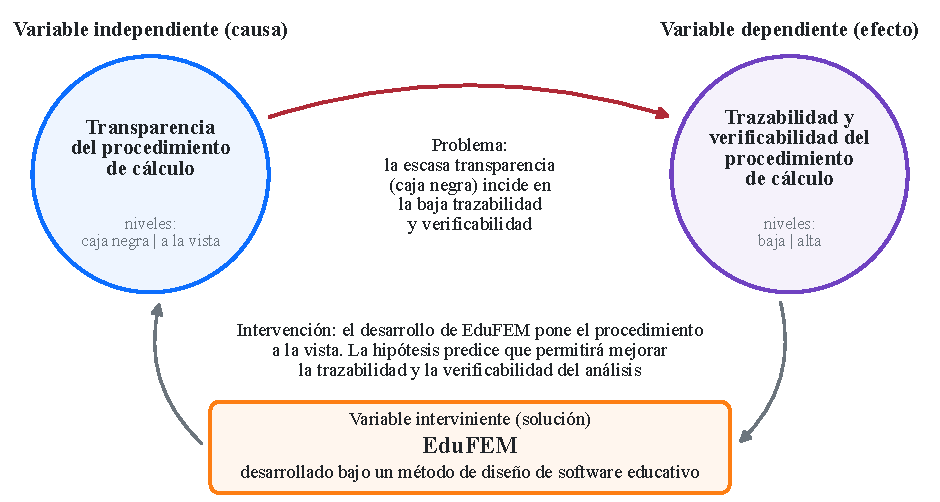
\includegraphics[width=\linewidth]{fig_relacion_variables.pdf}
\caption[Relación entre las variables de la investigación.]{Relación entre las variables de la investigación. Arriba, el problema: la escasa transparencia (caja negra) incide en la baja trazabilidad y verificabilidad. Abajo, la variable interviniente: EduFEM, desarrollado bajo un método de diseño de software educativo, pone el procedimiento a la vista, y la hipótesis predice que su desarrollo permitirá mejorar las dos propiedades.}
\label{fig:variables}
\end{figure}

Las magnitudes del experimento numérico no son variables del problema científico, y la tabla las distingue con otro nombre. Los \emph{factores} son la definición del modelo estructural y las decisiones de discretización: el tipo de elemento (Q4 o Q9) y la densidad de malla. Las \emph{magnitudes medidas} son la respuesta calculada y su exactitud frente a las referencias. El tipo de análisis y el orden de cuadratura se mantienen \emph{controlados} en cada configuración. El desempeño del solucionador se registra como \emph{observado}, sin criterio de aceptación, para documentar la escalabilidad del motor.

{\footnotesize
\setlength{\tabcolsep}{3pt}
\renewcommand{\arraystretch}{1.15}
\begin{longtable}{@{}>{\raggedright\arraybackslash}p{2.9cm}>{\raggedright\arraybackslash}p{2.5cm}>{\raggedright\arraybackslash}p{5.5cm}>{\raggedright\arraybackslash}p{2.7cm}@{}}
\caption[Operacionalización de las variables de la investigación.]{Operacionalización de las variables de la investigación: dimensiones, indicadores con que se mide cada una e instrumento que produce el dato. Sobre la raya, las variables de la investigación: las dos del problema científico y la interviniente; bajo ella, las magnitudes del experimento numérico, que no son variables del problema.}\label{tab:variables}\\
\toprule
\textbf{Variable} & \textbf{Dimensión} & \textbf{Indicador} & \textbf{Instrumento} \\
\midrule
\endfirsthead
\caption[]{Operacionalización de las variables de la investigación (continuación).}\\
\toprule
\textbf{Variable} & \textbf{Dimensión} & \textbf{Indicador} & \textbf{Instrumento} \\
\midrule
\endhead
\bottomrule
\endfoot
Independiente: transparencia del procedimiento de cálculo & Exposición de las etapas; interactividad; documentación & Magnitudes intermedias visibles en cada etapa; operación sobre el modelo del usuario en las tres fases; memoria de cálculo con sustitución numérica. Niveles: caja negra o procedimiento a la vista & Matriz de atributos (\autoref{tab:comparativa}); inventario de módulos \\
Dependiente: trazabilidad y verificabilidad del procedimiento de cálculo & Trazabilidad & Etapas con módulo educativo (de las siete primeras) y con desarrollo en la memoria (de nueve); solución y tensiones expuestas en el post-proceso; fases que comparten el lienzo (de tres); ítems del universo de contenido con instrumento (de dieciocho); formatos con ida y vuelta sin pérdida. Niveles de la variable: baja (solo datos y resultados finales) o alta & Inventario de módulos; memoria del ejemplo guía; tabla de cobertura de contenido; pruebas de consistencia interna \\
 & Verificabilidad & Tasa de convergencia observada frente a la teórica; error relativo de la flecha y de $\sigma_x$ frente a la solución analítica, y diferencia relativa frente a SAP2000; residuo de equilibrio; error en la membrana de Cook y firma del bloqueo por cortante; memoria reproducible a mano & Guiones de verificación y validación; modelo de SAP2000 (\autoref{anexo:sap2000}); \autoref{anexo:memoria} \\
Interviniente: EduFEM, desarrollado bajo un método de diseño de software educativo & Método aplicado; versión evaluada & Actividades del método ubicadas en el documento; decisiones de diseño trazadas a sus principios; EduFEM~1.0.0, revisión \texttt{91e3df0} & \autoref{tab:dsrm}; \autoref{tab:principios}; instalador y repositorio \\
\midrule
Factores del experimento numérico & Definición del modelo; discretización & Dominio y malla; $E$, $\nu$, espesor $t$; cargas y restricciones; Q4 o Q9; tamaño característico $h$ (o malla de $N\times N$ elementos) y número de GDL & Guion de cada caso \\
Magnitudes medidas & Respuesta; exactitud & $\sigma_x,\sigma_y,\tau_{xy},\sigma_{\mathrm{VM}}$; $u_x,u_y$ nodales; tasa de convergencia; normas del error del desplazamiento y de la tensión recuperada; error relativo (\%) frente a la solución analítica y diferencia relativa (\%) frente a SAP2000; residuo de la suma de reacciones & Solucionador; guiones de verificación y validación \\
Controlados & Tipo de análisis; integración & Tensión o deformación plana; orden de cuadratura & Constantes de cada configuración del guion \\
Observado: desempeño & Tiempo; memoria & Tiempos de ensamblaje y de solución; memoria de $\bm{K}$ densa y dispersa & Guion de medición de tiempos \\
\end{longtable}}

\subsection{Matriz de consistencia}
\label{sec:matriz-consistencia}

El \textbf{problema científico} es el enunciado único de la Introducción: ¿de qué manera la escasa transparencia del procedimiento de cálculo del software de análisis por elementos finitos podrá incidir en la baja trazabilidad y verificabilidad de ese procedimiento, en la gestión 2026? Se atiende con el \textbf{objetivo general}: desarrollar un software educativo de elementos finitos para el análisis estructural, empleando el lenguaje de programación Python, debido a la escasa transparencia del procedimiento de cálculo del software de análisis, para mejorar la trazabilidad y la verificabilidad del procedimiento de cálculo. Se contrasta con la \textbf{hipótesis}: «Bajo la aplicación de un método de diseño de software educativo, el desarrollo de EduFEM permitirá mejorar la trazabilidad y la verificabilidad del análisis por el Método de los Elementos Finitos en elasticidad plana, dada la escasa transparencia con que el software expone su procedimiento de cálculo». Los tres enunciados comparten sus variables: la independiente es en el problema la causa, en el objetivo general su porqué y en la hipótesis la situación dada; la dependiente es en los tres la trazabilidad y la verificabilidad, que la hipótesis atribuye al análisis realizado mediante el procedimiento de cálculo. La hipótesis se contrasta parte por parte ---sus premisas con evidencia documental, y su efecto en dos cláusulas: (a) trazabilidad y (b) verificabilidad--- según la \autoref{sec:validacion-resultados}. La \autoref{tab:consistencia} traza la correspondencia entre cada objetivo específico, la pregunta de investigación que responde, la variable o el indicador asociado, el método empleado y la evidencia que lo respalda en el documento.

\begin{table}[htbp]
\centering
\caption[Matriz de consistencia de la investigación.]{Matriz de consistencia: correspondencia entre objetivos específicos, preguntas de investigación (PI), variables, métodos y evidencia. Cada pregunta corresponde a una cláusula de la hipótesis: PI-1 a la (a), trazabilidad, y PI-2 a la (b), verificabilidad.}
\label{tab:consistencia}
{\footnotesize
\setlength{\tabcolsep}{3pt}
\renewcommand{\arraystretch}{1.15}
\begin{tabular}{@{}>{\raggedright\arraybackslash}p{3.0cm}>{\raggedright\arraybackslash}p{1.3cm}>{\raggedright\arraybackslash}p{3.0cm}>{\raggedright\arraybackslash}p{3.6cm}>{\raggedright\arraybackslash}p{2.7cm}@{}}
\toprule
\textbf{Objetivo específico} & \textbf{PI} & \textbf{Variable / indicador} & \textbf{Método / instrumento} & \textbf{Evidencia} \\
\midrule
1. Fundamentar el MEF en elasticidad plana y el estado del arte del software para su enseñanza & PI-1 y PI-2 & Etapas del procedimiento; atributos ausentes en los recursos existentes, que pasan a ser requisitos; criterios de verificación y validación & Revisión de los antecedentes y de la literatura clásica del MEF, de su verificación y validación y de su enseñanza; análisis comparativo & \autoref{cap:marco_teorico}; \autoref{tab:comparativa} \\
2. Desarrollar EduFEM: motor, interfaz, módulos y memoria & PI-1 & Variable independiente en su nivel de procedimiento a la vista; etapas expuestas; ida y vuelta de los formatos sin pérdida & Método de la ciencia del diseño (actividad 3): desarrollo iterativo con pruebas de regresión & \autoref{sec:diseno-edufem}; \autoref{sec:consistencia-interna}; \autoref{sec:cobertura-canal} \\
3. Verificar y validar EduFEM & PI-1 y PI-2 & Variable dependiente: trazabilidad (cobertura del procedimiento y del contenido) y verificabilidad (tasas, errores, equilibrio, bloqueo por cortante) & Inventario de módulos; tabla de cobertura de contenido; soluciones manufacturadas; viga de Timoshenko; membrana de Cook; SAP2000; ejemplo guía & \autoref{cap:resultados}; \autoref{anexo:memoria} \\
\bottomrule
\end{tabular}}
\end{table}

Las preguntas de investigación son las enunciadas en la Introducción, una por cláusula de la hipótesis. \textbf{PI-1} pregunta por la organización de la interfaz, de los módulos y de la memoria que permite seguir cada resultado hasta sus datos. \textbf{PI-2} pregunta por la exactitud del motor frente a soluciones exactas y referencias externas, y por la reproducción de los fenómenos numéricos que la teoría predice. El primer objetivo, la fundamentación, es transversal: sustenta las dos preguntas y se materializa en el \autoref{cap:marco_teorico}. El segundo construye lo que examina la PI-1, y el tercero responde a las dos. El intercambio de datos (DXF, CSV), parte del desarrollo, es un complemento instrumental de la trazabilidad: no origina una pregunta propia, pero sí un criterio de la cláusula (a), porque los resultados solo pueden seguirse hasta sus datos si el modelo entra y sale de la herramienta sin pérdida. Sus datos y su veredicto se reportan en la \autoref{sec:consistencia-interna}. Del mismo modo, que la memoria del ejemplo guía pueda rehacerse a mano no origina una pregunta propia, pero sí un criterio de la cláusula (b), porque permite comprobar cada etapa contra un cálculo manual.

\subsection{Población, muestra y casos de estudio}
\label{sec:poblacion}

La unidad de análisis es el procedimiento de cálculo del software, no las personas que lo usan. La \emph{población} es, por eso, el universo de problemas de elasticidad lineal plana —en tensión o en deformación plana— que pueden resolverse con elementos cuadriláteros isoparamétricos. La Carrera de Ingeniería Civil delimita el contexto de aplicación del trabajo; no es su población.

La \emph{muestra} no es estadística, sino dirigida: una selección intencional por valor probatorio \autocite[p.~215]{sampieri2018metodologia}. Es coherente con la práctica de la verificación de códigos de cálculo, donde los casos de prueba se eligen por su capacidad de ejercitar todos los términos del modelo matemático y por cubrir la malla más general que el código deberá resolver, antes que por su realismo físico \autocite[pp.~190, 208]{oberkampf2010vv}. Los casos de estudio son tres, y cada uno aporta una referencia de naturaleza distinta:

\begin{itemize}
    \item El \emph{método de soluciones manufacturadas} provee una solución exacta construida a propósito. Ejercita la fuerza de volumen, las restricciones no homogéneas y el mapeo sobre elementos distorsionados. Se corre en cuatro configuraciones: cuadrado unitario y cuadrilátero distorsionado, en tensión y en deformación plana. Recorre así las dos matrices constitutivas, aunque con el campo elegido solo es sensible a la diferencia entre dos de sus términos, $D_{11}-D_{12}$, que vale lo mismo en la \autoref{eq:D-tension-plana} y en la \autoref{eq:D-deformacion-plana} (\autoref{sec:mms}).
    \item La \emph{viga de Timoshenko} simplemente apoyada ejercita la carga superficial uniforme y los apoyos. Aporta dos referencias externas: una solución analítica de la teoría de la elasticidad y un modelo de cáscara en SAP2000.
    \item La \emph{membrana de Cook} ejercita la distorsión trapezoidal bajo cortante y flexión, el modo de deformación ante el que el elemento Q4 bloquea.
\end{itemize}

Entre los tres quedan cubiertos los términos del modelo de la \autoref{sec:formulacion-debil}: cargas de volumen y superficiales uniformes, restricciones homogéneas y no homogéneas, ambos elementos y la tensión plana. Hay tres excepciones, que se declaran. Las cargas nodales de la \autoref{eq:ensamblaje} solo intervienen en el ejemplo guía, que no mide exactitud. La carga superficial linealmente variable no interviene en ningún caso de estudio ni tiene contraste externo; las recomendaciones proponen un caso que la incorpore. Y la deformación plana solo interviene en las soluciones manufacturadas, que no la distinguen de la tensión plana (\autoref{sec:mms}), y no tiene contraste externo: la viga de Timoshenko y la membrana de Cook son de tensión plana. En su matriz constitutiva, una prueba de regresión sobre un estado de deformación uniaxial con solución cerrada acota, junto con las soluciones manufacturadas, los términos $D_{11}$ y $D_{12}$ (\autoref{tab:vyv-repro}); el de cortante, $D_{33}$, no tiene prueba propia. El refinamiento de malla y la comparación entre Q4 y Q9 se realizan en los dos casos con secuencia de mallas, el de soluciones manufacturadas y la membrana de Cook, ambos con $N\in\{2,4,8,16,32\}$ elementos por lado. La viga de Timoshenko se resuelve con una única malla fina de elementos Q9. Es un contraste puntual de exactitud frente a las dos referencias externas, no un estudio de convergencia. A los tres casos se suma el \emph{ejemplo guía}, un modelo de nueve nodos y cuatro elementos Q4 que acompaña al lector por todo el procedimiento y es el escenario sobre el que el \autoref{anexo:memoria} muestra que la memoria de cálculo puede reproducirse a mano.

Para la trazabilidad se define un \emph{universo de contenido}, que se recorre exhaustivamente y no por muestreo. Tiene dos partes. La primera son las nueve etapas del procedimiento de cálculo enumeradas en la \autoref{sec:variables-met}. La segunda son los contenidos que un consenso de 67 expertos de la industria y de la academia califica como necesarios para el egresado \autocite[pp.~1162-1163]{perezsantiago2023fem}. Las dos categorías de contenido de ese estudio reúnen 49 ítems: 15 conceptos teóricos (FEM1 a FEM15) y 34 destrezas prácticas (FEA1 a FEA34). De ellos se toman los 18 que pertenecen al procedimiento de cálculo y a su verificación dentro de la elasticidad plana:
\begin{itemize}
    \item quince destrezas: las seis de mallado (FEA13 a FEA18), las tres de post-proceso (FEA26 a FEA28), las tres de conceptos fundamentales (FEA29 a FEA31) y las tres de verificación y validación (FEA32 a FEA34); el mallado y la verificación y validación están entre las tres dimensiones que ese consenso califica más alto \autocite[p.~1168]{perezsantiago2023fem};
    \item tres conceptos: el ensamblaje con restricciones y solución (FEM2), la formulación isoparamétrica de elementos bidimensionales (FEM8) y la integración numérica de Gauss (FEM9).
\end{itemize}
Los 31 ítems restantes quedan fuera por tres motivos. Dieciocho caen fuera del alcance disciplinar: resortes, barras y vigas, elementos axisimétricos, análisis tridimensional, placas y cáscaras, problemas térmicos, modelado en CAD, cargas tomadas de un análisis previo, elementos rígidos y contacto. Doce son destrezas de planificación del análisis, de selección de materiales y de modelado de cargas y apoyos, que anteceden al procedimiento de cálculo. Y uno, la deducción de la matriz de rigidez por métodos alternativos (FEM3), es un desarrollo teórico que el software no expone. La \autoref{sec:contenido-didactico} los lista uno por uno.

\subsection{Procedimiento, instrumentos y reproducibilidad}
\label{sec:validacion-datos}

Cada caso numérico sigue el mismo procedimiento. Un guion construye la malla, define el material, las cargas y los apoyos, y llama directamente al solucionador del motor. El comprobador de salud (\autoref{sec:pre-proceso}), que en la interfaz revisa los datos antes de resolver y detiene el cálculo ante errores críticos, salvo que el usuario decida resolver de todos modos, no interviene en los guiones. En la verificación por soluciones manufacturadas, la consistencia de los datos se cumple por construcción: el término fuente se deduce analíticamente de la solución exacta elegida, y por eso las cargas y las restricciones corresponden exactamente a ella.

El sistema se ensambla y se resuelve con la versión vectorizada del motor; los módulos educativos y la memoria de cálculo exponen el cálculo con su versión legible, elemento a elemento, que una prueba de regresión mantiene coincidente con la primera (\autoref{sec:motor}). Lo que el software expone coincide así con lo que el motor calcula, dentro de la tolerancia de esa prueba. Las tensiones se recuperan por la secuencia descrita en la \autoref{sec:resolucion-tensiones}.

Los instrumentos de medición numérica son los guiones de verificación y validación del proyecto (\texttt{tests/vv\_mms.py}, \texttt{tests/vv\_timoshenko.py} y \texttt{tests/vv\_cook.py}). Computan las normas de error (integradas con la cuadratura de orden superior de la \autoref{sec:verificacion-validacion}), los errores relativos frente a las referencias y las tasas de convergencia, y depositan los datos en archivos CSV. Dentro de cada configuración solo se manipulan el tipo de elemento y la densidad de malla, fijos en la viga de Timoshenko; el método de soluciones manufacturadas varía, además, la geometría y el tipo de análisis entre sus cuatro configuraciones (\autoref{sec:poblacion}). En cada configuración, el tipo de análisis, el material, la geometría, las cargas y los apoyos, el orden de cuadratura ($2\times2$ para Q4 y $3\times3$ para Q9) y las tolerancias numéricas del motor permanecen fijos.

Los instrumentos de la trazabilidad son dos. El primero es el \emph{inventario de módulos}: la lista de las etapas del procedimiento con el módulo educativo, la sección de la memoria o la vista del post-proceso que expone cada una. El segundo es la \emph{tabla de cobertura de contenido}, que confronta, ítem por ítem, lo que el software ofrece con lo que el consenso de expertos exige. Cruza cada ítem del universo de la \autoref{sec:poblacion} con el instrumento del software que lo cubre y con la evidencia de este documento que lo respalda. La regla de marcado es una sola: un ítem se da por cubierto solo si el instrumento existe en la versión evaluada y la \autoref{sec:diseno-edufem} o el \autoref{anexo:manual} lo describen; en caso contrario, la celda queda vacía. A estos instrumentos se suma el análisis comparativo de la \autoref{tab:comparativa}, que sitúa el software frente a los recursos existentes.

La tabla de cobertura es una verificación de requisitos, no un juicio de expertos sobre el software. Los ítems del universo proceden de un consenso publicado; la selección, con los tres motivos de exclusión que declara la \autoref{sec:poblacion}, y el cotejo son del autor, y por eso cada celda remite a una función o a una captura que cualquier lector puede comprobar con el software instalado. El propio estudio advierte que sus resultados, obtenidos con expertos mexicanos de ingeniería mecánica, no son generalizables a otros contextos \autocite[p.~1171]{perezsantiago2023fem}. Lo que ese contexto condiciona es la importancia relativa que los expertos dan a cada ítem, y la tabla no pondera: solo registra si el ítem tiene o no instrumento. A ello se añade que los dieciocho ítems retenidos no son propios de una especialidad. El mallado, el post-proceso, los conceptos fundamentales, la verificación y la validación, la formulación isoparamétrica y la cuadratura de Gauss pertenecen al procedimiento de cálculo del MEF, que es el mismo en ingeniería civil y en ingeniería mecánica. Los ítems ligados a una tipología estructural o a un dominio ajeno al continuo plano —resortes, barras y vigas, elementos axisimétricos, placas y cáscaras, problemas térmicos— quedaron fuera del universo por esa misma razón.

La reproducibilidad se apoya, en lo numérico, en el determinismo del motor: ante las mismas entradas produce las mismas salidas, y cada caso se regenera por completo al ejecutar de nuevo su guion sobre la versión identificada en la \autoref{sec:proceso-met}. A ello se suma una batería de pruebas de regresión que verifica la estabilidad del modelo de datos ante operaciones de edición, y que se reporta en la \autoref{sec:consistencia-interna}.

\subsection{Criterios de aceptación y contraste de la hipótesis}
\label{sec:validacion-resultados}

La hipótesis afirma el efecto de una intervención bajo una condición y a partir de una situación dada. Se contrasta, por eso, en cuatro partes, en el orden de su enunciado:
\begin{enumerate}
    \item la \textbf{condición} («bajo la aplicación de un método de diseño de software educativo»), que se respalda con la \autoref{tab:dsrm} y la \autoref{tab:principios};
    \item la \textbf{intervención} («el desarrollo de EduFEM»), que lleva la variable independiente al nivel de procedimiento a la vista y se respalda con la versión evaluada (\autoref{sec:proceso-met}) y con la \autoref{tab:fases};
    \item el \textbf{efecto} («permitirá mejorar la trazabilidad y la verificabilidad del análisis»), que es la variable dependiente y se contrasta en dos cláusulas, una por dimensión;
    \item el \textbf{antecedente} («dada la escasa transparencia con que el software expone su procedimiento de cálculo»), que es la variable independiente en su nivel de partida y se respalda con la \autoref{tab:comparativa}.
\end{enumerate}
La condición, la intervención y el antecedente son premisas documentales: si el método no se hubiera aplicado, si EduFEM no expusiera su procedimiento o si el software de análisis ya expusiera el suyo, la hipótesis no podría contrastarse tal como está enunciada. El efecto es la parte que puede resultar falsa, y por eso lleva criterios de aceptación con umbral. Sus dos cláusulas son:
\begin{itemize}
    \item[(a)] \textbf{Trazabilidad.} Cada etapa del procedimiento de cálculo queda expuesta sobre el modelo del usuario: las siete primeras, en un módulo educativo; las nueve, en la memoria de cálculo; y la solución y las tensiones, además, en el post-proceso. Las tres fases del análisis operan sobre un mismo lienzo, y las entidades del modelo entran y salen de la herramienta, por los formatos de intercambio de datos, sin pérdida. Y el contenido expuesto cubre las destrezas y los conceptos que un consenso publicado de expertos exige, dentro del alcance del trabajo.
    \item[(b)] \textbf{Verificabilidad.} Frente a soluciones exactas construidas para la verificación, el error del motor decrece con las tasas de convergencia que predice la teoría. Sus resultados coinciden, dentro de las tolerancias fijadas, con la solución analítica de la viga de Timoshenko, con un modelo de SAP2000 y con el valor de referencia de la membrana de Cook, y sus reacciones equilibran la carga. Reproducen además el bloqueo por cortante del elemento Q4 ---su rigidez excesiva bajo flexión--- frente a la convergencia del Q9. Y la memoria de cálculo del ejemplo guía, el modelo de nueve nodos y cuatro elementos Q4 de la \autoref{sec:poblacion}, puede reproducirse a mano.
\end{itemize}
La hipótesis no es una tautología: exponer el procedimiento no asegura que lo expuesto esté completo ni que sea correcto. La regla de decisión es conjuntiva. Una cláusula se cumple si se cumplen todos sus criterios. La hipótesis queda comprobada si sus premisas se respaldan y se cumplen las dos cláusulas; parcialmente comprobada, si se cumple una sola; y no comprobada, si no se cumple ninguna. Si alguna premisa no se respaldara, el efecto no llegaría a juzgarse.

Los criterios numéricos de aceptación están escritos en los propios guiones de verificación y validación, que los evalúan automáticamente y terminan con error si alguno falla; el de intercambio de datos lo evalúan del mismo modo las pruebas que cita la \autoref{sec:consistencia-interna}. Los demás de trazabilidad y el del ejemplo guía son documentales, y los verifica el autor sobre la versión evaluada con la regla de marcado de la \autoref{sec:validacion-datos}. Ningún umbral numérico se escribió antes de las primeras corridas, ni se calculó a partir de sus resultados. Los de la flecha, de la membrana de Cook y de las tasas de convergencia se incorporaron a los guiones al comienzo de la verificación, cuando estos ya imprimían esos errores; los de $\sigma_x$ y del equilibrio, al final del desarrollo. Por eso el veredicto no descansa en el valor exacto de cada umbral, sino en el margen con que se cumple, que resume la \autoref{fig:margen-criterios}. La \autoref{tab:criterios} los reúne, con la procedencia de cada umbral y con el resultado que lo refutaría. En la cláusula (a), el inventario de módulos cubre las etapas 1 a 7 porque las dos últimas ---la solución del sistema y la recuperación de tensiones--- no tienen módulo propio y se exponen en el post-proceso, que la tercera fila audita con su propio criterio; las nueve se desarrollan en la memoria de cálculo.

{\footnotesize
\setlength{\tabcolsep}{3pt}
\renewcommand{\arraystretch}{1.15}
\begin{longtable}{@{}>{\raggedright\arraybackslash}p{2.3cm}>{\raggedright\arraybackslash}p{3.6cm}>{\raggedright\arraybackslash}p{2.6cm}>{\raggedright\arraybackslash}p{3.0cm}>{\raggedright\arraybackslash}p{2.3cm}@{}}
\caption[Criterios de aceptación con que se contrasta el efecto de la hipótesis.]{Criterios de aceptación con que se contrasta el efecto de la hipótesis, en sus dos cláusulas: magnitud observada, umbral, procedencia del umbral y resultado que refutaría la cláusula.}\label{tab:criterios}\\
\toprule
\textbf{Caso o instrumento} & \textbf{Magnitud} & \textbf{Umbral} & \textbf{Procedencia del umbral} & \textbf{Lo refutaría} \\
\midrule
\endfirsthead
\caption[]{Criterios de aceptación con que se contrasta el efecto de la hipótesis (continuación).}\\
\toprule
\textbf{Caso o instrumento} & \textbf{Magnitud} & \textbf{Umbral} & \textbf{Procedencia del umbral} & \textbf{Lo refutaría} \\
\midrule
\endhead
\bottomrule
\endfoot
\multicolumn{5}{@{}l}{\textbf{Cláusula (a): trazabilidad}} \\*
Inventario de módulos & Etapas 1 a 7 con módulo educativo & 7 de 7 & Exhaustividad & Una etapa sin módulo \\*
Memoria de cálculo & Etapas con desarrollo y sustitución numérica & 9 de 9 & Exhaustividad & Una etapa sin desarrollo \\*
Post-proceso & Solución y tensiones expuestas, en modo crudo y suavizado & Ambas & Exhaustividad & Una sin exposición \\*
Interfaz & Fases que operan sobre el mismo lienzo & 3 de 3 & Exhaustividad & Una fase en otra vista \\*
Tabla de cobertura & Ítems del universo de contenido con instrumento & 18 de 18 & Exhaustividad & Un ítem sin instrumento \\*
Intercambio de datos & Ida y vuelta CSV sin pérdida; importación DXF repetible; memoria generada para Q4 y Q9 & Sin pérdida y sin error & Exhaustividad & Una entidad perdida o un error \\
\midrule
\multicolumn{5}{@{}l}{\textbf{Cláusula (b): verificabilidad}} \\*
Soluciones manufacturadas & Tasa de convergencia del desplazamiento en norma $L^2$, cuatro configuraciones (\autoref{sec:verificacion-validacion}) & Teórica $\pm 0{,}5$ (2 en Q4 y 3 en Q9) & Medio orden: separa el orden esperado del inmediato inferior, que es el que produce un error de programación & Una tasa fuera de margen \\
Soluciones manufacturadas & Tasa de convergencia del desplazamiento en seminorma $H^1$, cuatro configuraciones & Teórica $\pm 0{,}5$ (1 en Q4 y 2 en Q9) & Medio orden, como en la fila anterior & Una tasa fuera de margen \\
Viga de Timoshenko & Error de la flecha central frente a la solución analítica & $< 3\,\%$ & Tolerancia de ingeniería fijada por el autor & Error mayor \\
Viga de Timoshenko & Error de $\sigma_x$ frente a la solución analítica, en los tres puntos de control de la \autoref{sec:timoshenko} & $< 1\,\%$ & Tolerancia de ingeniería fijada por el autor & Un valor mayor \\
Viga de Timoshenko & Diferencia de $\sigma_x$ frente a SAP2000, en los mismos tres puntos & $< 1\,\%$ & Tolerancia de ingeniería fijada por el autor & Un valor mayor \\
Viga de Timoshenko & Residuo relativo del equilibrio global de reacciones & $< 10^{-8}$ & Orden del cero numérico del motor & Residuo mayor \\
Membrana de Cook & Error del desplazamiento con Q9 y $N=8$, en valor absoluto & $< 1{,}5\,\%$ & Tolerancia de ingeniería fijada por el autor & Error mayor \\
Membrana de Cook & Flecha del Q4 menor que la del Q9 con la misma malla & Se observa & Predicción de la teoría: bloqueo por cortante & Que no se observe \\
Ejemplo guía & Etapas de la memoria desarrolladas con sustitución numérica y remitidas a su ecuación, de modo que puedan rehacerse a mano & Todas & Exhaustividad & Una etapa sin desarrollo cotejable \\
\end{longtable}}

Tres precisiones completan la tabla. Primera: las tasas de convergencia se juzgan en su valor asintótico, medido entre las dos mallas más finas ($N=16$ y $N=32$), porque en las mallas gruesas la tasa todavía no se ha estabilizado. Segunda: el autor fijó el criterio de la viga de Timoshenko sobre la tensión normal $\sigma_x$ porque es la magnitud primaria del problema de flexión. Las componentes secundarias se reportan, pero no forman parte del criterio: su magnitud en los puntos de control es muy inferior a la de $\sigma_x$, lo que agranda su error relativo (\autoref{sec:interpretacion}). Tercera: para la tensión recuperada en los nodos, cuya tasa teórica no está establecida para la secuencia de extrapolación y promediado que emplea el motor, el guion de soluciones manufacturadas incluye un umbral mínimo de 1,4 en Q4 y de 1,9 en Q9. El autor eligió ese umbral después de observar el comportamiento del motor. No es un criterio de aceptación de la hipótesis, sino una salvaguarda contra retrocesos al modificar el código. El desempeño del solucionador se reporta sin criterio de aceptación.

El efecto se contrasta cláusula por cláusula con esos criterios. La cláusula (a), trazabilidad, responde a PI-1 y se contrasta en la \autoref{sec:cobertura}, salvo el intercambio de datos, que se reporta en la \autoref{sec:consistencia-interna}. La cláusula (b), verificabilidad, responde a PI-2 y se contrasta en la \autoref{sec:mms}, la \autoref{sec:timoshenko} y la \autoref{sec:cook}, salvo el criterio del ejemplo guía, que se contrasta sobre la memoria del \autoref{anexo:memoria}. La condición, la intervención y el antecedente se respaldan con la evidencia documental de los Capítulos~1 a~3 que indica la lista del comienzo de esta subsección. La \autoref{sec:validacion-hipotesis} reúne los veredictos: criterio por criterio en una tabla, y parte por parte en otra.

\section{El software EduFEM}
\label{sec:diseno-edufem}

Definido el diseño metodológico, esta segunda parte del capítulo describe el diseño y la implementación de EduFEM, el software educativo de elementos finitos que materializa los fundamentos expuestos en el \autoref{cap:marco_teorico} y concreta el modelo de investigación. La exposición avanza desde los requisitos que motivaron las decisiones de arquitectura hasta el detalle de cada capa de la herramienta: las tecnologías empleadas, la organización por capas en torno a un modelo de proyecto mutable, el motor numérico, el pre-proceso interactivo, los módulos educativos, el post-proceso y la generación de documentación. El énfasis está puesto en \emph{cómo} se construyó cada componente, no en la teoría que lo respalda, que ya quedó establecida; y cada decisión de diseño se justifica aquí por lo que aporta a la trazabilidad o a la verificabilidad del análisis.

EduFEM resuelve el problema estático lineal de la elasticidad plana —tensión plana y deformación plana— con elementos isoparamétricos cuadriláteros de cuatro y nueve nodos, bajo la hipótesis de pequeños desplazamientos. Quedan fuera el análisis dinámico, la no linealidad del material o de la geometría y el dominio tridimensional, conforme a la delimitación establecida en la Introducción (\emph{Alcance y limitaciones}).

\subsection{Requisitos y decisiones de diseño}
\label{sec:requisitos}

El objetivo general enunciado en la Introducción ---desarrollar un software educativo de elementos finitos que mejore la trazabilidad y la verificabilidad del procedimiento de cálculo--- se traduce, en el plano de la herramienta, en una lista de requisitos que condicionó todas las decisiones posteriores. Esa lista no la fijó el autor por conveniencia: la produce el análisis de los antecedentes del \autoref{cap:marco_teorico}, que, a partir de la \autoref{tab:comparativa}, identifica los ocho atributos que ninguno de los recursos educativos revisados reúne a la vez. De ellos se derivan cinco requisitos:

\begin{enumerate}
    \item \textbf{Procedimiento de cálculo completo a la vista sobre el modelo del usuario.} Cada operación del método —mapeo isoparamétrico, matriz Jacobiana, matriz de deformación-desplazamiento, matriz constitutiva, integración numérica, ensamblaje, imposición de restricciones y recuperación de tensiones— debe poder inspeccionarse visual e interactivamente sobre la geometría que el propio usuario construyó, y no quedar oculta tras una caja negra.
    \item \textbf{Memoria de cálculo reproducible a mano.} El análisis debe quedar documentado con sustitución numérica paso a paso, sobre los valores del modelo del usuario, en un documento que pueda rehacerse con lápiz y papel o en una hoja de cálculo.
    \item \textbf{Exactitud verificada y validada, publicada junto con la herramienta.} Los resultados del motor deben contrastarse con soluciones exactas construidas para la verificación, con casos clásicos de la literatura y con un software comercial, dentro de tolerancias explícitas, y ese contraste debe publicarse con la herramienta, en su repositorio, y poder repetirse.
    \item \textbf{Cobertura del contenido que los expertos exigen.} Lo que la herramienta expone debe cubrir, dentro del alcance del trabajo, las destrezas y los conceptos del universo de contenido definido en la \autoref{sec:poblacion} a partir de un consenso publicado de expertos.
    \item \textbf{Software libre y en español.} La herramienta debe distribuirse sin licencias comerciales y con su código fuente disponible ---el de EduFEM se publica bajo licencia MIT---, y su interfaz y su documentación deben estar íntegramente en español.
\end{enumerate}

Los dos primeros requisitos sirven a la trazabilidad del procedimiento de cálculo, y el segundo y el tercero, a su verificabilidad; el cuarto extiende la trazabilidad al contenido que un consenso publicado de expertos califica como necesario, y el quinto pone una y otra al alcance del estudiante. Es la misma lista que la \autoref{tab:dsrm} registra como objetivos de la solución. El \autoref{cap:resultados} contrasta los cuatro primeros mediante los criterios de aceptación de la \autoref{tab:criterios}; las subsecciones que siguen remiten a la lista al justificar cada decisión de diseño.

Dos hallazgos de la literatura sobre enseñanza del método acompañan al primer requisito y orientaron su forma. El software educativo interactivo se reporta como conducente a una mejor comprensión de los conceptos del análisis estructural \autocite[p.~168]{lee2015interactive}, y la construcción paso a paso de las herramientas de cálculo junto con el estudiante resulta eficaz \autocite[p.~1023]{bishay2020teaching}. Uno y otro se refieren a las herramientas que sus autores evaluaron, y este trabajo no traslada a EduFEM lo que allí se reporta: el primero es una evaluación cualitativa, sin datos cuantitativos, y el segundo atribuye la mejora principalmente a que los propios estudiantes formulan sus problemas, y solo en parte a las herramientas computacionales (\autoref{sec:fundamentos-pedagogicos}). EduFEM no le pide al estudiante que formule problemas ni que escriba código; de ese segundo hallazgo solo se retiene lo que puede trasladarse a un programa de uso —que el procedimiento quede a la vista etapa por etapa y pueda reproducirse a mano—, que es justamente lo que enuncian los requisitos 1 y 2. En conjunto, ambos orientaron el diseño hacia la manipulación directa antes que hacia la mera lectura de resultados.

El autor adoptó tres decisiones generales para concretar estos requisitos en la herramienta. La primera es el \emph{idioma}: la interfaz, los mensajes del comprobador de salud y la documentación generada se redactan en español, con la terminología que el autor fijó para el proyecto (GDL en lugar de DOF, MEF en lugar de FEM, restricción en lugar de condición de contorno). En la versión evaluada quedan dos rótulos en inglés ---el contador «warning(s)» del comprobador de salud y la descripción «sparsity pattern» de M7 en el lanzador de módulos---, y la memoria de cálculo y los documentos de teoría conservan «condiciones de contorno». La segunda es la \emph{primacía de lo visual}: el modelo se construye y se consulta sobre el lienzo, con sincronización inmediata entre la representación tabular y la geométrica. La tercera es la \emph{independencia tecnológica}: EduFEM se apoya exclusivamente en software libre o en código propio, sin licencias comerciales, para que pueda distribuirse y ejecutarse en cualquier equipo de un laboratorio docente. Para facilitar su adopción en el aula, la herramienta se distribuye para Windows mediante un instalador que despliega el software como paquete autocontenido ---un lanzador empaquetado con \texttt{PyInstaller} y la carpeta con el intérprete de Python y todas las dependencias---; así, el estudiante no necesita instalar Python ni bibliotecas, y el código fuente permanece público para su inspección o extensión. El procedimiento detallado de instalación se describe en el \autoref{anexo:instalacion}.

La identidad visual de la herramienta sintetiza estos requisitos. El icono de EduFEM (\autoref{fig:logo-edufem}) fusiona sus dos planos: un birrete académico —que evoca su finalidad educativa— cuyo tablero es una malla de elementos finitos coloreada con la misma paleta que el post-proceso emplea para los campos de tensión. Así, la identidad gráfica y la salida del software comparten un lenguaje visual coherente.

\begin{figure}[H]
\centering

\includegraphics[width=0.30\linewidth]{fig_logo_edufem}
\caption[Icono de EduFEM.]{Icono de EduFEM. El birrete académico remite a la finalidad educativa de la herramienta, y su tablero es una malla de elementos finitos coloreada con la misma paleta de resultados con que el post-proceso presenta los campos de tensión (\autoref{sec:post-proceso}).}
\label{fig:logo-edufem}
\end{figure}

\subsection{Tecnologías empleadas}
\label{sec:stack}

La implementación se realizó íntegramente en Python, lenguaje que combina una sintaxis accesible con un ecosistema científico maduro. La \autoref{tab:stack} resume las bibliotecas adoptadas y su función dentro del sistema. La interfaz gráfica se construyó sobre \texttt{tkinter}, la biblioteca estándar de Python para interfaces de ventana, con un tema visual profesional aportado por \texttt{ttkbootstrap} (tema oscuro \emph{darkly}). El núcleo numérico se apoya en NumPy, que provee el álgebra densa, y en SciPy, que provee las matrices dispersas y el solucionador lineal \autocite{harris2020numpy,virtanen2020scipy}; las funciones de forma y la cuadratura de Gauss las implementa el propio motor, y no una biblioteca de elementos finitos de terceros.

\begin{table}[htbp]
\centering
\caption[Componentes de la plataforma de desarrollo de EduFEM.]{Componentes de la plataforma de desarrollo de EduFEM: la tecnología adoptada para cada función del sistema y el papel concreto que cumple dentro de él.}
\label{tab:stack}
\setlength{\tabcolsep}{4pt}
\begin{tabular}{@{}l >{\raggedright\arraybackslash}p{4.0cm} >{\raggedright\arraybackslash}p{6.9cm}@{}}
\toprule
\textbf{Función} & \textbf{Tecnología} & \textbf{Rol en el sistema} \\
\midrule
Interfaz gráfica      & \texttt{tkinter} + \texttt{ttkbootstrap} & Ventanas, tablas y menús (tema \emph{darkly}) \\
Cálculo numérico      & NumPy, SciPy                              & Álgebra densa y dispersa, solucionador disperso \\
Gráficos              & \texttt{matplotlib}                      & Vista tridimensional, círculo de Mohr y gráficos de los módulos \\
Cálculo simbólico     & \texttt{sympy}                           & Fórmulas de los módulos; integrando simbólico de M5 y de la memoria \\
Generación de PDF     & \texttt{pylatex} + \TeX{} Live embebido    & Memoria de cálculo paso a paso y documentos de teoría \\
Importación CAD       & \texttt{ezdxf}                            & Lectura de geometría desde archivos DXF \\
Imagen y figuras      & \texttt{Pillow}                           & Dibujo de los contornos y de las figuras de la memoria \\
Animación educativa   & \texttt{manim}                            & Generación de los videos didácticos en WebP, un formato de imagen que admite animación, prerrenderizados y distribuidos con la herramienta \\
Distribución          & \texttt{PyInstaller} + Inno Setup         & Paquete autocontenido e instalador único (Windows) \\
\bottomrule
\end{tabular}
{\singlespacing\notaapa{Todas las tecnologías listadas son de código abierto, conforme al requisito de software libre. Las bibliotecas de Python que viajan en el instalador llevan licencias permisivas —BSD, MIT o similares—, y \texttt{PyInstaller} se distribuye bajo GPL-2.0 con una excepción expresa que deja libre la licencia del programa empaquetado. \TeX{} Live reúne programas independientes con licencias libres propias, como la GPL del motor pdfTeX y la LPPL de los paquetes de \LaTeX{}; EduFEM los invoca como procesos separados, de modo que esas licencias no se extienden a su código. Por eso ninguna de estas licencias condiciona la de EduFEM: el código propio se publica bajo licencia MIT, y el paquete binario se redistribuye con los avisos de licencia de cada componente, que el instalador reúne en el archivo \texttt{LICENCIAS-TERCEROS.txt}. \texttt{manim} es la única que no acompaña a la herramienta instalada: es una herramienta de construcción, con la que los videos se generan antes de empaquetar y se distribuyen ya renderizados.}}
\end{table}

La generación de la memoria de cálculo se delega en \texttt{pylatex}, que compone el documento \LaTeX{} compilado luego por \texttt{pdflatex}. El mismo camino siguen los documentos de teoría que acompañan a los módulos educativos, y los dos PDF se abren con el visor del sistema: la herramienta no incorpora ninguna biblioteca de lectura de PDF. Para que esa compilación no dependa de que el estudiante instale por su cuenta una distribución \LaTeX{}, el instalador incorpora una copia reducida de \TeX{} Live —únicamente el motor \texttt{pdflatex} y los paquetes que usan la memoria y los documentos de teoría— que EduFEM localiza junto a su propio ejecutable antes de recurrir a cualquier instalación del sistema. La importación de geometría desde formatos CAD recae en \texttt{ezdxf}, el dibujo de las figuras del PDF y de los contornos en \texttt{Pillow}, y la producción de los videos didácticos en \texttt{manim}. El autor evitó deliberadamente toda dependencia de bibliotecas multimedia pesadas: los videos se reproducen como WebP animado decodificado por \texttt{Pillow}, lo que reduce el tamaño del instalador distribuible.

Estas elecciones no son indiferentes al propósito del trabajo. Escribir el motor sobre bibliotecas numéricas de propósito general, en lugar de adoptar un paquete de elementos finitos ya hecho, es lo que deja disponibles las matrices intermedias para exponerlas y documentarlas, como piden los requisitos 1 y 2. Y que todas las piezas sean libres y viajen dentro del instalador —incluido el compilador \LaTeX{}— es lo que permite que cualquiera genere la memoria de cálculo sin licencias, sin conexión y sin instalaciones previas, como pide el requisito 5. Las comprobaciones del \autoref{cap:resultados}, en cambio, no viajan en el instalador: se repiten desde el repositorio público, con el código fuente y los guiones que enumera el \autoref{anexo:vyv}, como pide el requisito 3.

\subsection{Arquitectura por capas en torno al modelo de proyecto}
\label{sec:arquitectura}

EduFEM adopta un patrón de tipo Modelo--Vista--Controlador (MVC) organizado en capas: el estado del análisis, su presentación en pantalla y la lógica que los conecta viven en piezas separadas. La pieza central es la clase \texttt{ProjectModel}. Este objeto concentra el estado completo del análisis —nodos, elementos, materiales, cargas, restricciones, configuración del problema y, tras resolver, la solución— y se comparte por referencia con todos los componentes, de modo que todos trabajan sobre el mismo estado. Cada capa de la \autoref{tab:capas} cumple una responsabilidad acotada. El motor de cálculo (\texttt{fem/}) no depende de ninguna capa de interfaz; la interfaz y los módulos educativos, en cambio, se apoyan unos en otros. La \autoref{fig:arquitectura} ilustra el flujo entre capas.

\begin{table}[H]
\centering
\caption[Capas de la arquitectura de EduFEM.]{Capas de la arquitectura de EduFEM: el paquete de código que materializa cada capa y la responsabilidad que tiene asignada. El motor (\texttt{fem/}) no depende de ninguna capa de interfaz, y por eso puede ejecutarse sin pantalla.}
\label{tab:capas}
\begin{tabular}{@{}l >{\raggedright\arraybackslash}p{12.1cm}@{}}
\toprule
\textbf{Capa (paquete)} & \textbf{Responsabilidad} \\
\midrule
\texttt{models/}    & Modelo de proyecto, entidades, comprobación de salud, deshacer/rehacer \\
\texttt{fem/}       & Motor numérico del MEF (NumPy y SciPy; SymPy solo para el integrando simbólico) \\
\texttt{gui/}       & Interfaz: pre-proceso, lienzo y post-proceso \\
\texttt{education/} & Módulos educativos interactivos M0 a M7 \\
\texttt{file\_io/}  & Entrada/salida: proyecto, CSV, DXF y memoria PDF \\
\texttt{config/}    & Constantes, sistemas de unidades y paletas de color \\
\bottomrule
\end{tabular}
\end{table}

\begin{figure}[H]
\centering
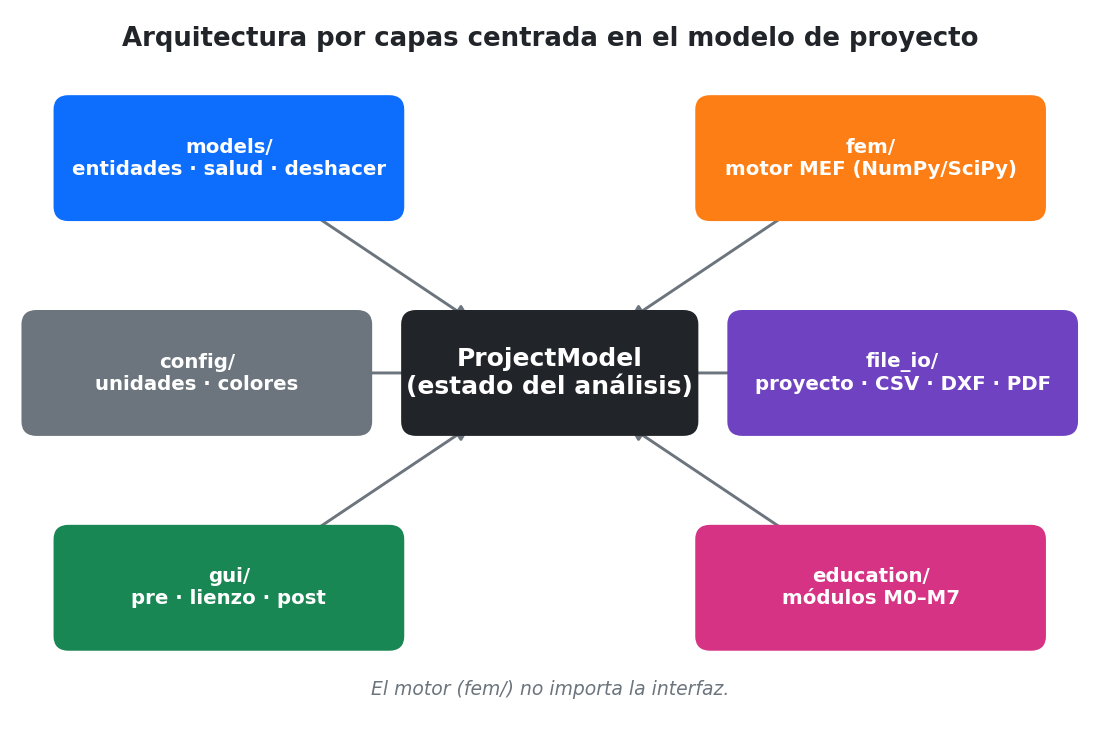
\includegraphics[width=0.92\linewidth]{fig_arquitectura}
\caption[Arquitectura por capas centrada en el modelo de proyecto.]{Arquitectura por capas de EduFEM en torno al modelo de proyecto. Los seis paquetes de código rodean al objeto \texttt{ProjectModel}, que concentra el estado del análisis y se comparte por referencia. La interfaz, el deshacer y la entrada y salida lo leen y lo modifican; el motor y los módulos educativos solo lo leen, y la configuración le aporta constantes. El motor (\texttt{fem/}) no importa ninguna biblioteca de interfaz.}
\label{fig:arquitectura}
\end{figure}

Toda mutación originada por la interfaz se aplica sobre el mismo objeto \texttt{ProjectModel}, que marca su estado como modificado y como no resuelto; de ese modo los cambios se propagan sin replicar datos. La configuración global del análisis —tipo de elemento, tipo de análisis (tensión plana o deformación plana), sistema de unidades y gravedad— reside también en el modelo y se guarda junto con la geometría.

Que el estado viva en un solo objeto y que el motor no dependa de la interfaz es lo que sostiene la trazabilidad del análisis. Los módulos educativos, la memoria de cálculo y los guiones de verificación leen el mismo modelo y calculan con el mismo paquete \texttt{fem/}: los guiones, con las funciones que resuelven el sistema; los módulos y la memoria, con su versión legible, que una prueba de regresión mantiene coincidente con aquellas (\autoref{sec:motor}). Lo expuesto al estudiante coincide así con lo que el motor calcula, y no es una ilustración preparada aparte.

\subsection{Separación entre identidad del nodo e índice de grado de libertad}
\label{sec:identidad-gdl}

Una decisión de diseño crítica es la separación explícita entre la \emph{identidad} de un nodo y su \emph{índice} en el sistema algebraico. El identificador de nodo es una etiqueta pública: es el número que el estudiante ve en la tabla y en el lienzo, y el que aparece en los archivos exportados y en la memoria de cálculo. Solo cambia si el usuario lo edita, y entonces el cambio se propaga a todas sus referencias; borrar otros nodos no lo altera, de modo que el conjunto de identificadores puede presentar huecos, por ejemplo $\{1, 5, 50\}$. El índice, en cambio, es interno: cada nodo recibe un ordinal $i$ en el rango $0$ a $N-1$, donde $N$ es el número de nodos, y sus dos grados de libertad (GDL) ocupan las posiciones $2i$ y $2i+1$ —de $0$ a $2N-1$— en la matriz $\bm{K}$, en el vector $\bm{F}$ y en la solución $\bm{u}$. La correspondencia entre uno y otro la resuelve un \emph{mapa de índices}\footnote{En el código, ese mapa es \texttt{node\_index\_map}, y las funciones auxiliares que lo consultan son \texttt{dof\_x} y \texttt{dof\_y}; el \autoref{anexo:codigo} indica dónde lo consulta el ensamblaje.}, que se construye bajo demanda a partir de los identificadores ordenados y se descarta al agregar, borrar o renombrar nodos, para que nunca quede desactualizado.

Esta separación tiene una consecuencia directa: la matriz de rigidez se dimensiona como $2N$ y no como $2\,\max(\text{identificador})$. Calcular el índice de un GDL como $2(\text{identificador}-1)$ —patrón ingenuo que asume identificadores contiguos— produce errores de indexación cuando el usuario elimina nodos intermedios, pues los identificadores dejan de ser consecutivos mientras el sistema algebraico permanece compacto. El acceso se realiza, por eso, siempre a través del mapa de índices. Separar la numeración que ve el usuario de la numeración interna de ensamblaje es, además, lo que permite que el modelo admita identificadores arbitrarios sin penalizar el tamaño del sistema: el costo de la indirección se reduce a una consulta en el mapa. Dimensionar $\bm{K}$ según el identificador máximo, en cambio, desperdiciaría memoria y dejaría filas y columnas nulas, que vuelven singular el sistema.

Esta separación es, en la práctica, una condición de la trazabilidad del análisis. Gracias a ella, el número de nodo que el estudiante lee en la interfaz ---tabla, lienzo y módulo M7--- y en la memoria de cálculo designa siempre al mismo nodo, aunque en el ínterin se hayan borrado o renumerado otros. Las filas y columnas de $\bm{K}$ que M7 resalta al ensamblar pueden seguirse, además, en sentido inverso hasta ese nodo y hasta el elemento que las aportó. Si identidad e índice se confundieran, el número visible y la posición en el sistema podrían dejar de referirse a la misma entidad, y ningún resultado sería rastreable hasta sus datos. La \autoref{sec:consistencia-interna} ejercita la separación con identificadores no contiguos.

\subsection{Motor de cálculo del MEF}
\label{sec:motor}

El paquete \texttt{fem/} concentra el motor numérico y observa una regla de pureza estricta: no importa ninguna biblioteca de interfaz gráfica, de modo que puede ejecutarse sin pantalla, por ejemplo en los guiones de verificación. El cálculo se organiza como una cadena de operaciones que van de la evaluación de las funciones de forma a la integración de la rigidez elemental por cuadratura de Gauss, según la \autoref{eq:ke-gauss}, con el espesor $t$ de cada elemento. Las aportaciones elementales se acumulan en la matriz global y el sistema reducido, una vez impuestas las restricciones, se resuelve con el solucionador disperso de SciPy. La formulación teórica detallada de cada una de estas operaciones —funciones de forma de los elementos Q4 y Q9, regla de la cadena para $\bm{B}$, expresiones de $\bm{D}$ en tensión y deformación plana, y la cuadratura de Gauss-Legendre— se desarrolló en el \autoref{cap:marco_teorico}. El \autoref{anexo:codigo} reproduce el código con que el motor evalúa las funciones de forma y ensambla la matriz global, para que cada expresión del marco teórico pueda cotejarse con las líneas que la calculan. Aquí interesa subrayar que el motor conserva dos versiones de ese cálculo, construidas sobre las mismas funciones de forma, la misma regla de Gauss y la misma matriz constitutiva. La que resuelve el sistema evalúa todos los elementos a la vez, con operaciones sobre arreglos; la versión legible recorre un elemento y un punto de Gauss por vez, y es la que usan los módulos educativos y la memoria de cálculo para exponer el procedimiento. Una prueba de regresión exige que ambas coincidan, de la rigidez elemental a las tensiones nodales, con un error relativo no mayor que $10^{-9}$ (\texttt{tests/test\_solver\_regression.py}). Esa prueba, y no la construcción, respalda la coherencia numérica entre lo que la herramienta explica y lo que resuelve.

Dos decisiones de implementación completan lo que el \autoref{cap:marco_teorico} deja abierto. La primera es un umbral geométrico: antes de ensamblar, el motor evalúa el determinante Jacobiano de cada elemento en sus puntos de Gauss y rechaza el elemento si, en alguno de ellos, el valor absoluto no supera el mínimo fijado en la configuración de la herramienta\footnote{La constante se llama \texttt{JACOBIAN\_MIN\_DETERMINANT} y se declara en el archivo de configuración, junto a la tolerancia numérica general del motor.}. El umbral detecta el elemento degenerado, pero no el signo: la rigidez se integra con $\lvert\det\bm{J}\rvert$ (\autoref{eq:ke-gauss}), y un determinante negativo no detiene el cálculo. Por eso lo acompañan otros dos controles, que avisan sin bloquear la resolución. El comprobador de salud advierte, por el área signada de los cuatro vértices, cuando la numeración es horaria. La evaluación de calidad clasifica como malo el elemento con Jacobiano escalado negativo, y el módulo M0 lo calcula en las esquinas, donde detecta el vértice entrante que el muestreo interior puede no ver. Entre los tres cubren la degeneración, la inversión de la numeración y la concavidad, aunque solo el primero detiene el cálculo; la biyectividad del mapeo en todo el dominio del elemento no se certifica punto a punto, sino que se infiere de esos controles.

La segunda es la forma de resolver el sistema, que se enuncia aquí en llano porque el \autoref{cap:resultados} vuelve sobre ella. La matriz de rigidez es casi toda ceros, porque cada nodo solo se relaciona con los nodos de sus propios elementos; se la llama por eso \emph{dispersa}, y el motor guarda únicamente sus coeficientes no nulos, cada uno con su fila y su columna, en lugar de reservar memoria para los $2N \times 2N$ valores. Resolver el sistema por \emph{factorización} consiste en descomponer esa matriz en dos matrices triangulares cuyo producto la reproduce; con ellas, los desplazamientos se obtienen por sustitución directa, primero hacia adelante y después hacia atrás, sin invertir ninguna matriz. El inconveniente de factorizar una matriz dispersa es que los factores suelen tener más coeficientes no nulos que ella —lo que se conoce como llenado—, así que antes de factorizar se reordenan las incógnitas con un criterio de mínimo grado, que elimina primero las ecuaciones con menos conexiones y evita buena parte de ese llenado. EduFEM emplea la factorización LU dispersa de la biblioteca SuperLU, a través de SciPy \autocite[p.~264]{virtanen2020scipy}, con el ordenamiento de mínimo grado calculado sobre $\bm{K}^{T}+\bm{K}$, que aprovecha la simetría estructural de la matriz\footnote{Es la opción \texttt{MMD\_AT\_PLUS\_A} del parámetro \texttt{permc\_spec} de la función \texttt{spsolve} de \texttt{scipy.sparse.linalg}, documentada en la propia biblioteca. La alternativa genérica, que no aprovecha esa simetría, es el ordenamiento de columnas de mínimo grado aproximado (COLAMD).}; el \autoref{cap:resultados} cuantifica su efecto frente al ordenamiento genérico.

Una y otra decisión sirven al mismo fin: el umbral protege la verificabilidad, porque ningún elemento degenerado en sus puntos de Gauss llega a ensamblarse, y el esquema disperso mantiene el costo del análisis dentro de lo que una computadora de aula resuelve, sin alterar en nada las matrices que los módulos educativos y la memoria de cálculo exhiben.

\subsection{Pre-proceso interactivo}
\label{sec:pre-proceso}

El pre-proceso permite construir el modelo combinando una entrada tabular y una entrada gráfica, ambas operando sobre el mismo proyecto. La entrada tabular se organiza como una hoja de cinco tablas —nodos, elementos, cargas, restricciones y cargas superficiales— con edición por doble clic, copiado y pegado en texto separado por tabulaciones, el formato con que las hojas de cálculo copian y pegan sus celdas, y filas de marcador de posición para agregar registros con valores por omisión. Los encabezados muestran las unidades activas y se actualizan al cambiar el sistema de unidades.

La entrada gráfica se realiza sobre un \emph{lienzo único y compartido} entre las tres fases del trabajo: pre-proceso, proceso y post-proceso superponen sus visualizaciones sobre el mismo lienzo en lugar de intercambiarlo. Sobre él se ofrece un modo de dibujo de elementos al estilo de un programa CAD: el usuario marca los cuatro vértices, con anclaje (\emph{snap}) a los nodos existentes para no duplicarlos, y al marcar el cuarto el lienzo cierra el cuadrilátero; si la orientación resultante es horaria, invierte el orden antes de crear el elemento. La \autoref{fig:lienzo-lod} muestra el lienzo durante esta operación.

\begin{figure}[H]
\centering
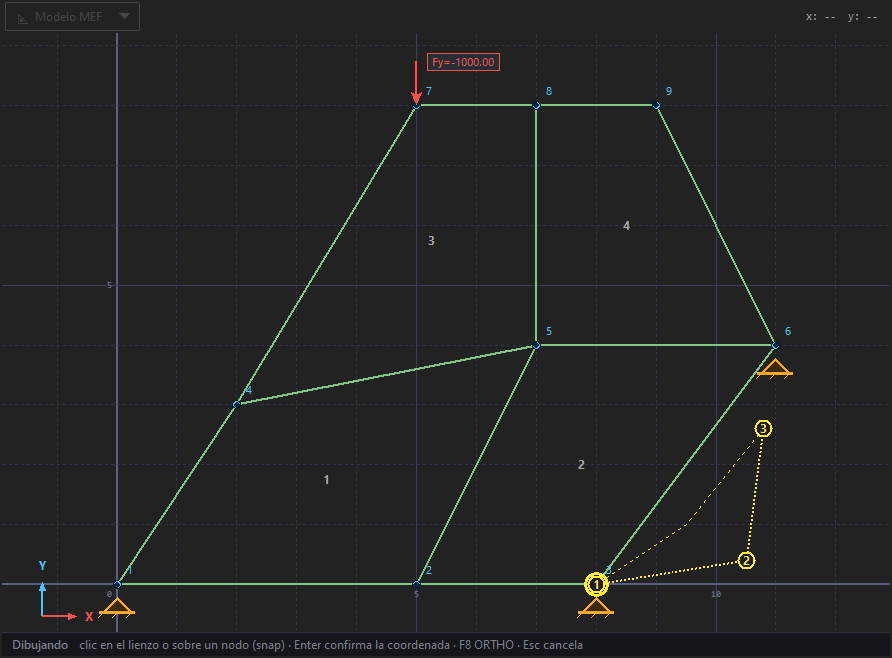
\includegraphics[width=0.82\linewidth]{fig_lienzo_lod}
\caption[Lienzo compartido durante el modo de dibujo.]{Lienzo compartido de EduFEM durante el modo de dibujo, sobre un modelo de nueve nodos y cuatro elementos Q4. Los vértices 1, 2 y 3 marcados en amarillo son los que el usuario ya fijó, y la línea punteada anticipa el cuadrilátero que se cerrará al confirmar el cuarto. Se dibujan la numeración de nodos y elementos, la carga (flecha roja) y los apoyos (triángulos naranjas); en un modelo de este tamaño, el dibujo se mantiene completo a cualquier acercamiento.}
\label{fig:lienzo-lod}
\end{figure}

La sincronización entre lienzo y tabla es bidireccional: seleccionar un elemento en la tabla lo resalta en el lienzo, y seleccionar entidades en el lienzo reconstruye la selección en la tabla y, cuando corresponde, propone filas tentativas para cargas o restricciones sobre las entidades elegidas. El lienzo aplica además, en las mallas de más de doce elementos, un \emph{nivel de detalle} dependiente del acercamiento: con la malla alejada solo se dibujan la silueta del dominio y la selección activa, y al acercarse aparecen los nodos intermedios, las etiquetas y la numeración. En los modelos menores, como el ejemplo guía, el dibujo se mantiene completo a cualquier acercamiento.

Las acciones del usuario son reversibles mediante un mecanismo de deshacer y rehacer basado en \emph{instantáneas}, es decir, copias del estado del modelo en un instante dado: antes de cada operación se captura el estado copiándolo a una estructura de datos independiente, y al deshacer se restaura ese mismo estado sobre el objeto original, sin crear uno nuevo\footnote{Los métodos son \texttt{to\_dict} y \texttt{restore\_from\_dict} de la clase \texttt{ProjectModel}.}. Como las instantáneas no incluyen la solución, sino solo la geometría y los datos del modelo, son pequeñas, y una acción del usuario equivale siempre a una instantánea, con independencia de cuántas modificaciones internas dispare.

La integridad del modelo se vigila con un comprobador de salud: una rutina que solo lee el proyecto, sin modificarlo, y reporta hallazgos clasificados en tres severidades. Los errores detienen la resolución: el usuario los corrige o decide expresamente resolver de todos modos, opción que no existe cuando faltan los elementos o las restricciones. Entre ellos están la ausencia de elementos, un nodo referenciado inexistente, un elemento degenerado y menos de tres GDL restringidos, el mínimo para suprimir los movimientos de cuerpo rígido. Las advertencias no bloquean el cálculo (cargas sobre nodos sin elemento, materiales sin uso, Jacobiano negativo por orientación horaria), y la información reúne contadores del modelo; el catálogo completo de chequeos está en la \autoref{tab:health-checks}. Parte de los hallazgos admite corrección automática: el diálogo de salud permite aplicarla, navegar hasta la entidad afectada y consultar una explicación del problema.

Los umbrales de calidad geométrica con que la memoria de cálculo y el módulo M0 clasifican los elementos son convención de la herramienta, apoyada en los mínimos que la biblioteca Verdict fija para el cuadrilátero (\autoref{sec:calidad-malla}). Los cortes no son los mismos en todas partes. El estado de calidad con que la memoria de cálculo clasifica cada elemento ---buena, aceptable o mala--- combina cuatro índices, y son los que la \autoref{tab:umbrales} enumera con su significado y sus dos cortes. El módulo M0, en cambio, endurece por prudencia el corte del Jacobiano escalado para su propio coloreado: lo eleva de $0{,}30$ a $q_{SJ} \ge 0{,}50$ —el valor que Verdict fija para el triángulo y el hexaedro— y distingue como buenos los elementos con $q_{SJ} \ge 0{,}80$ y compacidad $q_C \ge 0{,}50$. La razón es didáctica: en un curso introductorio conviene señalar como inadmisible un elemento que la biblioteca todavía toleraría. La memoria, por su parte, usa ese mismo corte de $0{,}50$ para colorear los valores de $q_{SJ}$ y para calificar globalmente la malla, sin cambiar por ello el estado de cada elemento.

\begin{table}[H]
\centering
\caption[Índices de calidad geométrica y cortes con que EduFEM clasifica cada elemento.]{Índices de calidad geométrica y cortes con que EduFEM asigna el estado global de cada elemento. Un elemento recibe calidad «Buena» si cumple los cuatro cortes de esa columna, «Aceptable» si cumple los cuatro de la siguiente, y «Mala» en cualquier otro caso.}
\label{tab:umbrales}
\setlength{\tabcolsep}{4pt}
\begin{tabular}{@{}>{\raggedright\arraybackslash}p{3.3cm} >{\raggedright\arraybackslash}p{6.6cm} cc@{}}
\toprule
\textbf{Índice} & \textbf{Qué mide} & \textbf{Buena} & \textbf{Aceptable} \\
\midrule
Jacobiano escalado $q_{SJ}$ & Cuánto se aparta el elemento de tener ángulos rectos, evaluado en los puntos de Gauss; vale $1$ en un cuadrado & $\ge 0{,}70$ & $\ge 0{,}30$ \\
Razón de Jacobianos $R_J$ & Uniformidad del mapeo dentro del elemento: cociente entre el menor y el mayor determinante Jacobiano & $\ge 0{,}50$ & $\ge 0{,}20$ \\
Relación de aspecto $AR$ & Cuánto se alarga el elemento; vale $1$ en un cuadrado o en un rombo & $\le 3$ & $\le 5$ \\
Estrechamiento $T_R$ & Trapecialidad: es nulo en todo paralelogramo y crece cuando las aristas opuestas dejan de ser paralelas & $\le 0{,}30$ & $\le 0{,}50$ \\
\midrule
Desviación de los nodos intermedios (solo Q9) & Apartamiento de los nodos de arista y central respecto de su posición ideal; sustituye al estrechamiento & $\le 0{,}10$ & $\le 0{,}25$ \\
\bottomrule
\end{tabular}
{\singlespacing\notaapa{Las definiciones de los cuatro índices están en la \autoref{sec:calidad-malla}. Los cortes no son umbrales tomados de la bibliografía, sino convención de la herramienta apoyada en los mínimos de Verdict.}}
\end{table}

La geometría puede importarse también desde archivos DXF, el formato de intercambio de los programas de dibujo asistido. EduFEM convierte sus polilíneas cerradas en elementos cuadriláteros según la convención de capas que adoptó el autor, documentada en el \autoref{anexo:formatos}. La importación puede repetirse sin efectos acumulados: los nodos se funden por proximidad —una estructura auxiliar agrupa los puntos por su posición y evita comparar cada nodo con todos los demás— y los elementos se reconocen por el conjunto de identificadores de sus nodos, de manera que reimportar el mismo archivo no genera duplicados. Como en el modo de dibujo, la orientación de cada cuadrilátero se fuerza a sentido antihorario calculando el área con signo. Esa orientación es condición necesaria, pero no suficiente: en un cuadrilátero no convexo el determinante Jacobiano puede resultar negativo en algún punto de Gauss aun con los vértices bien ordenados. El motor no detiene ese caso, porque solo rechaza el elemento cuyo $\lvert\det\bm{J}\rvert$ no supera el umbral mínimo (\autoref{sec:motor}); lo señala la evaluación de calidad de malla, que lo clasifica como malo.

Todo el pre-proceso sirve a una misma condición: que el modelo sobre el que después se expone el procedimiento sea válido y sea del propio usuario. El comprobador de salud señala los datos inconsistentes antes de resolver y detiene la resolución ante los errores, salvo decisión expresa del usuario; las dos vías de entrada, la tabla y el lienzo, permiten construir el mismo problema desde los números o desde el dibujo (requisitos 1 y 3).

\subsection{Módulos educativos}
\label{sec:educacion}

El componente educativo de EduFEM consiste en ocho módulos, numerados de M0 a M7, que recorren en orden el procedimiento de cálculo del MEF. No son ocho por conveniencia de implementación: cada uno corresponde a una etapa del procedimiento o a un contenido del universo definido en la \autoref{sec:poblacion}, que reúne esas etapas y lo que un consenso publicado de expertos califica como necesario, y la \autoref{sec:contenido-didactico} contrasta la cobertura una por una (requisito 4). Cada módulo se presenta como una \emph{capa superpuesta} interactiva: un panel flotante y arrastrable, acompañado de una iluminación que se dibuja directamente sobre la malla real del proyecto, sin abrir una representación auxiliar desconectada. La \autoref{tab:modulos} asocia cada módulo con la etapa del método que ilustra, y la \autoref{fig:modulo-capa} muestra el aspecto general de una de estas capas.

\begin{table}[H]
\centering
\caption[Los ocho módulos educativos de EduFEM.]{Los ocho módulos educativos de EduFEM: el concepto que expone cada uno y la etapa del procedimiento de cálculo a la que corresponde. M0 opera en el pre-proceso sobre la malla completa; M1 a M7 siguen, dentro de la fase de proceso, el orden del cálculo.}
\label{tab:modulos}
\begin{tabular}{@{}cll@{}}
\toprule
\textbf{Módulo} & \textbf{Concepto} & \textbf{Etapa del método} \\
\midrule
M0 & Calidad de malla        & Comprobación geométrica previa \\
M1 & Mapeo isoparamétrico    & Funciones de forma y coordenadas naturales \\
M2 & Jacobiano               & Distorsión local y $\det\bm{J}$ \\
M3 & Matriz $\bm{B}$         & Relación deformación--desplazamiento \\
M4 & Matriz constitutiva $\bm{D}$ & Comportamiento del material \\
M5 & Rigidez $\bm{k}_e$ + Gauss & Integración numérica de la rigidez \\
M6 & Fuerzas equivalentes    & Cargas distribuidas a fuerzas nodales \\
M7 & Ensamblaje              & Construcción de $\bm{K}$ y $\bm{F}$ globales \\
\bottomrule
\end{tabular}
\end{table}

\begin{figure}[H]
\centering
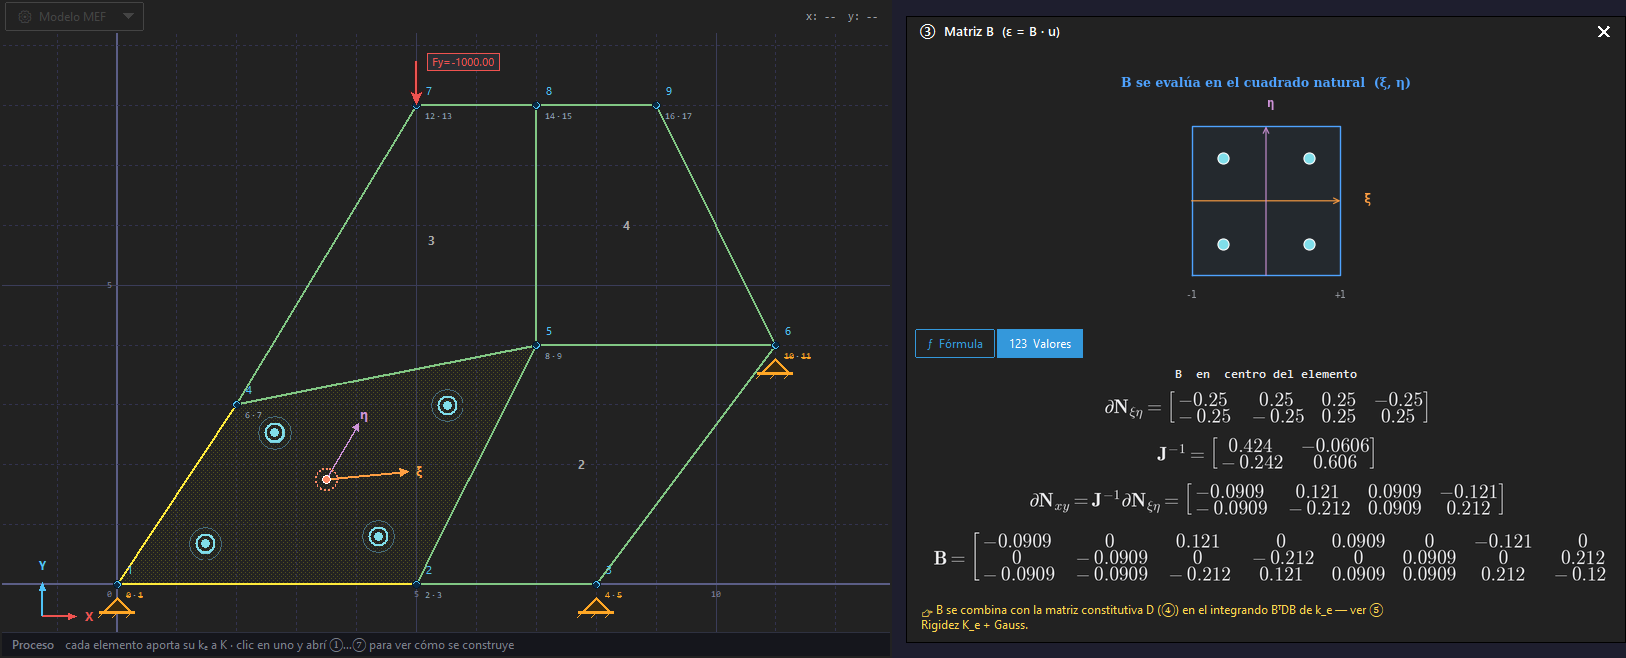
\includegraphics[width=0.86\linewidth]{fig_modulo_capa}
\caption[Módulo educativo como capa interactiva sobre el lienzo.]{El módulo M3 (matriz de deformación $\bm{B}$) como capa interactiva sobre el lienzo. A la izquierda, el elemento seleccionado con sus cuatro puntos de Gauss resaltados y los ejes naturales $\xi\eta$ dibujados en el punto evaluado; a la derecha, el panel flotante con la secuencia $\partial\bm{N}_{\xi\eta} \to \bm{J}^{-1} \to \partial\bm{N}_{xy} \to \bm{B}$ evaluada en ese punto y el conmutador entre la fórmula simbólica y sus valores numéricos. Todos los módulos comparten la capa sobre el lienzo y el panel flotante; el conmutador, en cambio, es propio de M2, M3 y M4.}
\label{fig:modulo-capa}
\end{figure}

El diseño de estos módulos parte de lo que Lee reporta sobre la interactividad en sus propios simuladores del MEF \autocite[pp.~158, 166]{lee2015interactive} —una evaluación cualitativa, sin grupo de control (\autoref{sec:fundamentos-pedagogicos})— y lo lleva a una filosofía minimalista que es decisión de este trabajo, y no un resultado tomado de la literatura. Cada módulo muestra lo mínimo necesario para que el concepto se lea sobre la geometría real. La selección del elemento bajo estudio se realiza con un solo clic sobre el lienzo, sin controles redundantes dentro del panel. La iluminación —resplandor sobre los puntos de Gauss, arcos de medición, coloreado por calidad— se aplica a la geometría real para preservar el contexto. La información matemática se concentra en el panel flotante, que en los módulos de las matrices $\bm{J}$, $\bm{B}$ y $\bm{D}$ alterna entre la fórmula simbólica y su evaluación numérica en el punto elegido.

M0 colorea cada elemento según su calidad y permite distorsionar un vértice para ver el efecto en vivo sin alterar el modelo. M5 contrapone la integral exacta de la rigidez, que no tiene primitiva practicable en un elemento de geometría arbitraria, con su aproximación por cuadratura: es esa impracticabilidad la que obliga a la cuadratura de Gauss, y el módulo la hace visible dejando agregar o quitar puntos de Gauss y observar el crecimiento de $\bm{k}_e$. M7 resalta las filas y columnas de $\bm{K}$ que recibe cada elemento al ensamblarse. Solo una capa educativa permanece activa a la vez, y abrir un módulo cierra el anterior: la regla evita que dos representaciones compitan por el mismo lienzo y hace que, por construcción, lo resaltado sobre la malla corresponda siempre a una sola etapa del procedimiento. El manual de uso reproduce cada uno de los ocho módulos en funcionamiento sobre el ejemplo guía, de la \autoref{fig:mod-m0} a la \autoref{fig:mod-m7} (\autoref{sec:catalogo-modulos-edu} del \autoref{anexo:manual}).

\subsection{Post-proceso}
\label{sec:post-proceso}

Resuelto el sistema, el post-proceso presenta los resultados sobre el mismo lienzo compartido. El campo de tensiones o de desplazamientos se dibuja como un contorno de color continuo: cada elemento se divide en triángulos y el color de cada punto de la pantalla se interpola a partir de valores nodales, de modo que el degradado no muestra escalones dentro del elemento\footnote{Es la interpolación conocida como sombreado de Gouraud, calculada con coordenadas baricéntricas sobre cada triángulo.}. En el modo suavizado, el predeterminado, esos valores son los de los cuatro nodos de esquina, también en el Q9. Sobre ese campo puede superponerse la malla deformada, dibujada en estilo alámbrico con un factor de escala configurable y la geometría original atenuada como referencia. La \autoref{fig:post-proceso} reúne estas vistas.

\begin{figure}[htbp]
\centering
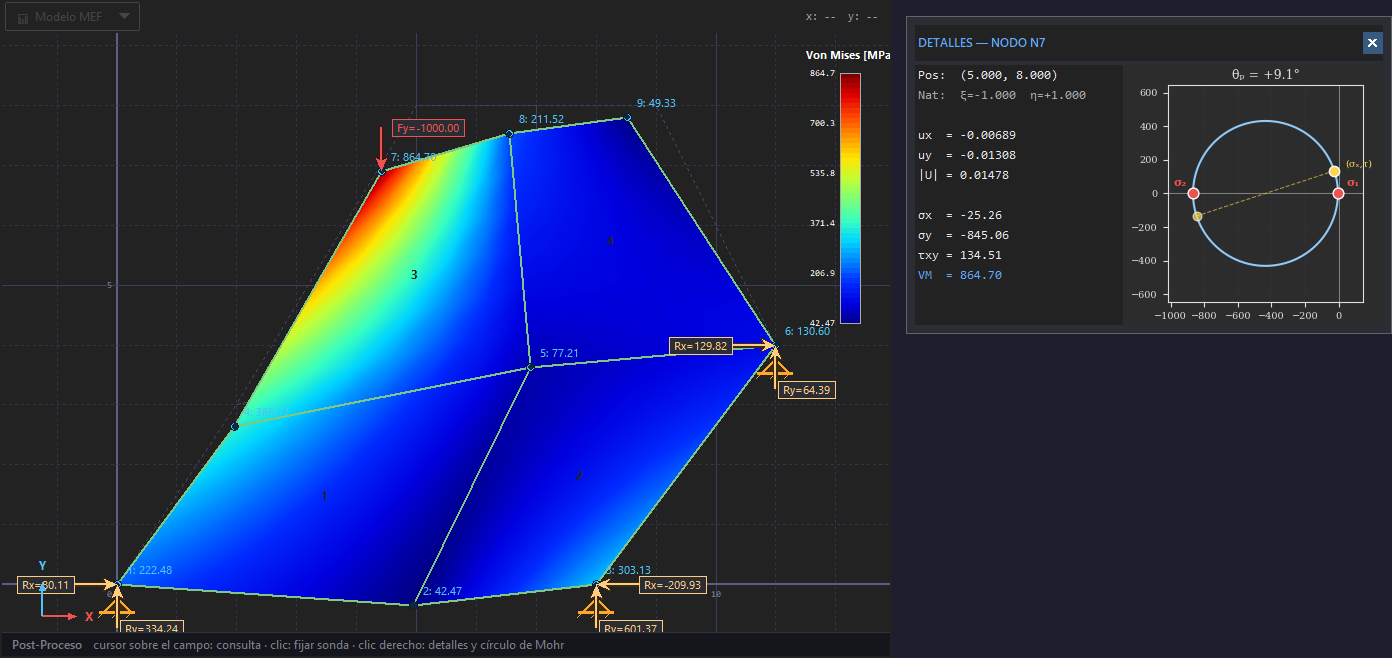
\includegraphics[width=\linewidth]{fig_postproceso}
\caption[Visualización de resultados en el post-proceso.]{Post-proceso de EduFEM sobre el modelo de cuatro elementos Q4. En el lienzo, el contorno continuo de la tensión de von Mises con su escala graduada, el valor nodal rotulado junto a cada nodo y las reacciones en los apoyos; a la derecha, el panel de la sonda puntual con el estado tensional del nodo consultado y su círculo de Mohr. El color da el orden de magnitud; el valor exacto se lee en el rótulo del nodo o en el panel.}
\label{fig:post-proceso}
\end{figure}

La inspección detallada se realiza con una sonda puntual: al consultar un punto cualquiera del dominio, EduFEM lo localiza dentro de su elemento mediante un mapeo inverso y abre un panel con los valores numéricos del estado tensional ---componentes cartesianas y von Mises---. Los acompaña un círculo de Mohr que sitúa las tensiones principales y el punto consultado en el plano tensional. Además, una vista tridimensional representa el campo como superficie sobre el dominio, y permite alternar entre la versión cruda, discontinua entre elementos, y la versión suavizada por promediado nodal. Todas las representaciones de campo emplean la paleta de color \emph{jet}. El autor la eligió por el reconocimiento inmediato que tiene en el ámbito de la ingeniería: es la paleta de tipo arcoíris con que se presentan habitualmente los mapas de tensiones en el software de análisis estructural. Y la eligió a sabiendas de su principal inconveniente: los mapas de tipo arcoíris no son perceptualmente uniformes —el ojo percibe fronteras nítidas donde el campo varía suavemente, sobre todo en el tránsito del cian al verde— y resultan poco accesibles para quien tiene visión cromática deficiente. Se privilegió la continuidad visual con las herramientas que el estudiante encontrará previsiblemente en la práctica profesional, supuesto que este trabajo no verifica, y el inconveniente se compensa con la escala numérica graduada junto al contorno y con la sonda puntual, que dan el valor exacto allí donde el color solo sugiere un rango. El \autoref{anexo:manual} ilustra estas vistas del post-proceso, incluida la representación tridimensional del campo (\autoref{fig:vista3d}).

\subsection{Memoria de cálculo e intercambio de datos}
\label{sec:memoria-io}

EduFEM genera una memoria de cálculo en PDF que documenta el análisis paso a paso. El documento se compone con \texttt{pylatex} y se compila con \texttt{pdflatex}, y ofrece dos estilos que comparten un mismo procedimiento de generación: un estilo \emph{educativo}, que enriquece el desarrollo con infografías, tarjetas de entrada y salida por capítulo, fórmulas al margen y un glosario final, y un estilo \emph{directo}, que presenta el mismo desarrollo matricial escuetamente para quien solo necesita comprobar el cálculo. La regla que gobierna ambos es que las fórmulas, matrices y ecuaciones se emiten siempre, mientras que únicamente la prosa explicativa y las cajas didácticas quedan condicionadas al estilo educativo.

El cuerpo del documento se estructura en nueve capítulos que reproducen el procedimiento de cálculo:
\begin{enumerate}
    \item planteo del problema;
    \item discretización del modelo;
    \item calidad de la malla;
    \item formulación elemental;
    \item ensamblaje del sistema global;
    \item imposición de restricciones y solución, capítulo que el documento rotula \textsf{Condiciones de contorno y solución};
    \item post-proceso: tensiones y deformada;
    \item diagnóstico del modelo, que el documento rotula \textsf{Diagnóstico y validación del modelo};
    \item resumen e interpretación de resultados.
\end{enumerate}
El desarrollo exhibe la secuencia de sustitución numérica completa, desde las funciones de forma evaluadas en los puntos de Gauss hasta la recuperación de tensiones y su promediado, recalculada con la versión legible del motor, la misma que usan los módulos educativos, lo que asegura por construcción su consistencia con ellos. El desarrollo íntegro de todos los elementos se emite mientras el modelo no supere dos elementos Q4 o uno Q9; por encima de ese tamaño, la memoria desarrolla el elemento de mayor energía de deformación y advierte que los demás se calculan igual. La matriz de rigidez global se imprime término a término hasta 18 GDL; por encima se muestra su patrón de entradas no nulas, y en todos los casos se reportan su número de entradas no nulas, su densidad y su ancho de banda.

El intercambio de datos con otras herramientas —la interoperabilidad, en el vocabulario de la informática— se resuelve por dos vías. El proyecto se guarda en formato propio \texttt{.edufem}, un archivo de texto JSON que contiene el volcado completo del modelo y se escribe atómicamente: primero en un archivo temporal, que solo se renombra al destino final una vez volcado a disco, para que un corte durante el guardado nunca deje el archivo corrupto. Para la edición masiva, el modelo se exporta e importa como un conjunto de archivos CSV, uno por entidad, agrupados en un ZIP, con encabezados que declaran las unidades y protección frente a la inyección de fórmulas en las celdas ---texto que una hoja de cálculo podría ejecutar como fórmula al abrir el archivo---. Ambos formatos contemplan la compatibilidad con versiones anteriores del proyecto, completando con valores por omisión los campos ausentes en archivos antiguos. El \autoref{anexo:formatos} documenta la estructura de los tres formatos —el proyecto \texttt{.edufem}, el paquete de archivos CSV y el DXF de importación— clave por clave y archivo por archivo.

Estas dos piezas cierran el recorrido del análisis. La memoria de cálculo es lo que hace trazable y verificable el resultado fuera de la pantalla: entrega el procedimiento completo con sus magnitudes intermedias, en un documento que puede rehacerse a mano, igual que la memoria con que se acompaña un cálculo estructural en la práctica profesional (requisitos 1 y 2). En los modelos mayores, esas magnitudes son las de un elemento representativo y el patrón de $\bm{K}$. Los formatos de intercambio, por su parte, permiten que las entidades del modelo salgan de la herramienta y vuelvan a ella sin pérdida, de manera que un mismo caso pueda resolverse y comprobarse también con otro programa (requisito 3); la \autoref{sec:consistencia-interna} verifica esa ida y vuelta.

\chapter{Verificación y validación de EduFEM mediante la medición de la cobertura de su procedimiento de cálculo y de la exactitud de su motor frente a soluciones exactas y referencias externas, para establecer si ese procedimiento es trazable y verificable}
\label{cap:resultados}
\chaptermark{Verificación y validación}% nombre corto para el pie de página


Este capítulo cumple el tercer objetivo específico: presenta y analiza los resultados de la verificación y la validación de EduFEM, según el diseño metodológico de la \autoref{sec:metodologia}. La evidencia es de dos clases, una por cada dimensión de la variable dependiente. La \emph{verificabilidad} se establece con evidencia numérica: se somete a EduFEM a una batería de verificación y validación, en la acepción que fija la \autoref{sec:verificacion-validacion}. La \emph{trazabilidad} se establece con evidencia documental: el inventario de lo que el software expone y la tabla de cobertura de contenido de la \autoref{sec:validacion-datos}.

Los datos y las figuras se reproducen ejecutando los guiones \texttt{tests/vv\_mms.py}, \texttt{tests/vv\_timoshenko.py} y \texttt{tests/vv\_cook.py} sobre la versión identificada en la \autoref{sec:proceso-met}, como detalla la \autoref{sec:vyv-reproducibilidad}.

\section{Medición de los datos y confiabilidad de la medición}
\label{sec:medicion}

Las dos variables del problema científico se observan en el software. La independiente —la transparencia del procedimiento de cálculo— se observa con los indicadores de exposición de las etapas, interactividad y documentación de la \autoref{tab:variables}, que reporta la \autoref{sec:cobertura-canal}. La dependiente se observa en sus dos dimensiones: la trazabilidad, en esa misma sección y en la \autoref{sec:contenido-didactico}; y la verificabilidad, con tres familias de indicadores numéricos que se describen a continuación.

La \emph{exactitud frente a soluciones de referencia} se cuantifica con la norma $L^2$ del desplazamiento, la seminorma $H^1$ del desplazamiento ---la norma $L^2$ de su gradiente--- y la norma $L^2$ del campo de tensiones recuperado, el que el post-proceso muestra, en sus formas absoluta y relativa. Se cuantifica también con los errores relativos porcentuales en tensión y desplazamiento respecto de los valores analíticos o de referencia. La \emph{respuesta estructural} se registra como desplazamientos nodales, componentes cartesianas de tensión, tensiones principales y de von Mises, y reacciones en los apoyos, cuya suma se contrasta con la carga total como comprobación de equilibrio. La \emph{convergencia} se mide como la tasa con que decrecen las normas de error al refinar la malla, estimada por el logaritmo en base dos del cociente de errores entre dos mallas sucesivas.

La confiabilidad de estas mediciones se respalda por tres vías. En primer lugar, las normas de error se integran con la cuadratura de orden superior de la \autoref{sec:verificacion-validacion}, para no subestimar el error. En segundo lugar, las tensiones se evalúan en los puntos de Gauss de cada elemento y se extrapolan a los nodos, según la \autoref{sec:resolucion-tensiones}. En tercer lugar, la corrección de ese operador de extrapolación se comprueba por separado, exigiendo que reproduzca exactamente los campos polinómicos de su espacio de interpolación; esa prueba forma parte de la batería de regresión, y la \autoref{sec:leccion-extrapolacion} cuenta por qué se incorporó. Los instrumentos de medición numérica son los guiones de verificación y validación del proyecto, deterministas y reejecutables: cada dato reportado puede repetirse. La confiabilidad de los instrumentos documentales descansa en que cada celda de sus tablas remite a una función descrita en la \autoref{sec:diseno-edufem}, a una captura del \autoref{anexo:manual} o a una prueba de la batería de regresión, que cualquier lector puede rehacer sobre el software distribuido; su limitación, declarada en la \autoref{sec:validacion-datos}, es que las construye el autor.

\section{Verificación numérica por el método de soluciones manufacturadas}
\label{sec:mms}

El método de soluciones manufacturadas (MMS), que describe la \autoref{sec:verificacion-validacion}, verifica el código comparando su resultado con una solución exacta construida a propósito. Si la implementación es correcta, el error debe disminuir con el tamaño característico de malla $h$ a las tasas asintóticas allí establecidas: $\mathcal{O}(h^{p+1})$ en la norma $L^2$ y $\mathcal{O}(h^{p})$ en la seminorma $H^1$, con $p$ el orden polinómico del elemento.

El autor adoptó como configuración base el cuadrado unitario $[0,1]^2$ en tensión plana, con material $E = 1{,}0$, $\nu = 0{,}3$ y espesor $t = 1{,}0$, y eligió como solución manufacturada

\begin{equation}
u_M(x,y) = \sin(\pi x)\,\sin(\pi y), \qquad v_M(x,y) = \cos(\pi x)\,\cos(\pi y),
\label{eq:mms-solucion}
\end{equation}
cuyo término fuente $\bm{b} = -\nabla\cdot\bm{\sigma}(\bm{u}_M)$, con $\bm{u}_M = (u_M, v_M)$, se inyecta como fuerza de volumen, y los valores de $\bm{u}_M$ se imponen como restricciones de Dirichlet no homogéneas en el contorno. EduFEM resolvió mallas estructuradas de $N\times N$ elementos para $N\in\{2,4,8,16,32\}$ en cuatro configuraciones: el cuadrado unitario y un cuadrilátero distorsionado de vértices $(0;\ 0)$, $(1;\ 0{,}15)$, $(0{,}85;\ 1)$ y $(0{,}1;\ 0{,}8)$ —cuyos elementos tienen Jacobiano no constante—, cada uno en tensión plana y en deformación plana, con el término fuente deducido en cada caso de la ley constitutiva correspondiente. Con este campo, la traza de la deformación y la distorsión angular son nulas en todo punto: la tensión exacta y el término fuente solo dependen de la diferencia $D_{11}-D_{12}$ de la matriz constitutiva, que vale $E/(1+\nu)$ en los dos estados planos (\autoref{eq:D-tension-plana} y \autoref{eq:D-deformacion-plana}). En todas ellas el guion de verificación midió la norma $L^2$ y la seminorma $H^1$ del desplazamiento y la norma $L^2$ del campo de tensiones recuperado $\bm{\sigma}^*_h$ (extrapolado a los nodos, promediado e interpolado con las funciones de forma, tal como lo muestra el post-proceso), integradas con la cuadratura de orden superior que justifica la \autoref{sec:verificacion-validacion}. La \autoref{tab:mms} reporta la configuración base; las otras tres se resumen en la \autoref{tab:mms-configs} del \autoref{anexo:vyv}.

La \autoref{tab:mms} reúne los errores y las tasas de convergencia observadas para ambos tipos de elemento. La tasa se calcula como el logaritmo en base dos del cociente de errores entre dos mallas sucesivas, puesto que cada refinamiento divide $h$ a la mitad. La tasa que se contrasta con el criterio es la asintótica, medida entre las dos mallas más finas ($N=16$ y $N=32$), porque en las mallas gruesas todavía no se ha estabilizado.

\begin{table}[htbp]
\centering
\caption[Errores absolutos y tasas de convergencia medidas por MMS (configuración base).]{Errores absolutos y tasas de convergencia medidas por MMS para los elementos Q4 y Q9 en la configuración base (cuadrado unitario, tensión plana): norma $L^2$ y seminorma $H^1$ del desplazamiento y norma $L^2$ del campo de tensiones recuperado $\bm{\sigma}^*_h$, abreviado $\sigma^*$ en los encabezados.}
\label{tab:mms}
\small
\setlength{\tabcolsep}{4pt}
\begin{tabular}{c r r c r c r c}
\hline
$N$ & GDL & error $L^2$ & tasa $L^2$ & error $H^1$ & tasa $H^1$ & error $\sigma^*$ & tasa $\sigma^*$ \\
\hline
\multicolumn{8}{l}{\textbf{Q4 (bilineal, $p=1$)}} \\
2  & 18   & $2{,}559\times10^{-1}$ & ---  & $1{,}496$               & ---  & $1{,}106$              & ---  \\
4  & 50   & $7{,}240\times10^{-2}$ & 1,82 & $7{,}247\times10^{-1}$  & 1,05 & $4{,}780\times10^{-1}$ & 1,21 \\
8  & 162  & $1{,}866\times10^{-2}$ & 1,96 & $3{,}578\times10^{-1}$  & 1,02 & $1{,}686\times10^{-1}$ & 1,50 \\
16 & 578  & $4{,}699\times10^{-3}$ & 1,99 & $1{,}783\times10^{-1}$  & 1,01 & $5{,}751\times10^{-2}$ & 1,55 \\
32 & 2178 & $1{,}177\times10^{-3}$ & 2,00 & $8{,}906\times10^{-2}$  & 1,00 & $1{,}976\times10^{-2}$ & 1,54 \\
\hline
\multicolumn{8}{l}{\textbf{Q9 (bicuadrático, $p=2$)}} \\
2  & 50   & $2{,}172\times10^{-2}$ & ---  & $2{,}911\times10^{-1}$  & ---  & $2{,}282\times10^{-1}$ & ---  \\
4  & 162  & $2{,}776\times10^{-3}$ & 2,97 & $7{,}263\times10^{-2}$  & 2,00 & $6{,}076\times10^{-2}$ & 1,91 \\
8  & 578  & $3{,}479\times10^{-4}$ & 3,00 & $1{,}809\times10^{-2}$  & 2,01 & $1{,}540\times10^{-2}$ & 1,98 \\
16 & 2178 & $4{,}352\times10^{-5}$ & 3,00 & $4{,}516\times10^{-3}$  & 2,00 & $3{,}860\times10^{-3}$ & 2,00 \\
32 & 8450 & $5{,}441\times10^{-6}$ & 3,00 & $1{,}129\times10^{-3}$  & 2,00 & $9{,}654\times10^{-4}$ & 2,00 \\
\hline
\end{tabular}
{\singlespacing\notaapa{Los errores son absolutos y, como los datos de la configuración base, carecen de unidades; los relativos del desplazamiento están en la \autoref{tab:mms-rel}, y el del campo de tensiones en la malla más fina, en la \autoref{tab:mms-configs}. Cada tasa se calcula con los errores sin redondear y puede diferir en una centésima de la que se obtiene con los valores impresos.}}
\end{table}

El elemento Q4 alcanza asintóticamente tasas de $\mathcal{O}(h^{2{,}00})$ en $L^2$ y $\mathcal{O}(h^{1{,}00})$ en $H^1$, que coinciden con la predicción teórica para un elemento de orden $p=1$; el elemento Q9 alcanza $\mathcal{O}(h^{3{,}00})$ en $L^2$ y $\mathcal{O}(h^{2{,}00})$ en $H^1$, igualmente coincidentes con la teoría para $p=2$. La aproximación progresiva de las tasas a su valor asintótico ---por ejemplo, el Q4 pasa de 1,82 en el primer refinamiento ($N=2$ a $N=4$) a 2,00 en el último ($N=16$ a $N=32$)--- es la firma esperada del régimen de convergencia. Las mismas tasas, con diferencias inferiores a 0,01, se obtienen en las otras tres configuraciones (\autoref{tab:mms-configs}): la deformación plana y la distorsión de los elementos no alteran el orden de convergencia, lo que descarta errores de orden en el ensamblaje, la integración por cuadratura de Gauss, el mapeo isoparamétrico sobre elementos no rectangulares y la imposición de restricciones no homogéneas. La matriz constitutiva queda fuera de ese alcance. Con el campo elegido solo interviene a través de $D_{11}-D_{12}$, que vale lo mismo en los dos estados planos, de modo que esta verificación no distinguiría la matriz de deformación plana de la de tensión plana. Una prueba de regresión con solución cerrada acota, junto con esta verificación, los términos $D_{11}$ y $D_{12}$ de la matriz de deformación plana: en un estado de deformación uniaxial, la tensión de von Mises depende de esos dos términos y de $\sigma_z$, y la prueba falla si en deformación plana se usa la matriz de tensión plana (\autoref{tab:vyv-repro}). El término de cortante, $D_{33}$, que en tensión plana ejercita la membrana de Cook, no tiene en deformación plana una prueba propia: solo puede comprobarse a mano, cotejando con la \autoref{eq:D-deformacion-plana} su expresión en el listado del \autoref{anexo:codigo} o los valores de $\bm{D}$ que muestran el módulo M4 y la memoria de cálculo de un modelo en deformación plana.

El campo de tensiones recuperado converge a $\mathcal{O}(h^{2{,}00})$ en el Q9 y a $\mathcal{O}(h^{1{,}54})$ en el Q4, por encima del orden $\mathcal{O}(h^{1})$ del gradiente crudo (seminorma $H^1$). Esas dos cifras son asintóticas: se miden entre las dos mallas más finas, igual que las del desplazamiento. El primer refinamiento, de $N=2$ a $N=4$, arroja todavía 1,21 en el Q4 y 1,91 en el Q9, valores que no están en régimen asintótico y que por eso no entran en el contraste. Medidas así, ambas tasas quedan por encima del mínimo de 1,4 en el Q4 y de 1,9 en el Q9 que exige el guion de soluciones manufacturadas. Ese mínimo no es un criterio de aceptación de la hipótesis, sino una salvaguarda contra retrocesos al modificar el código, que el autor eligió después de observar el comportamiento del motor (\autoref{sec:validacion-resultados}).

Ese orden del Q4 es una observación propia de este trabajo sobre la secuencia de muestreo en los puntos de Gauss, extrapolación y promediado nodal que emplea el motor (\autoref{sec:resolucion-tensiones}): la literatura consultada no fija un orden para esa secuencia, y Cook advierte que el promediado nodal simple no mejora por sí mismo la exactitud en su ejemplo \autocite[p.~231]{cook2002concepts}. Una explicación plausible de que no alcance $\mathcal{O}(h^{2})$, que este trabajo no contrastó, es la capa de contorno, donde los nodos reciben el promedio de un solo lado y pierden la cancelación de errores que los nodos interiores obtienen de sus cuatro elementos vecinos; comprobarla exigiría recomputar la norma $L^2$ del campo de tensiones excluyendo la franja de contorno. Esta verificación tiene límites: como en un campo suave los cuatro valores de Gauss de un elemento fino difieren en $\mathcal{O}(h)$, una permutación errónea de las columnas de la matriz de extrapolación apenas altera la norma $L^2$ en el régimen asintótico, aunque corrompa gravemente las tensiones nodales de una malla gruesa. Por eso la batería incluye la prueba de reproducción exacta de campos polinómicos, que comprueba el operador de extrapolación con independencia del tamaño de malla. La \autoref{sec:leccion-extrapolacion} refiere un defecto de ese tipo que existió en este mismo trabajo y sus consecuencias.

La \autoref{fig:convergencia} muestra las curvas de error del desplazamiento en escala doble logarítmica, donde la pendiente de cada recta corresponde a la tasa de convergencia; la \autoref{fig:convergencia-tension} muestra la del campo de tensiones recuperado.

\begin{figure}[htbp]
\centering
\begin{minipage}{0.49\linewidth}
  \centering
  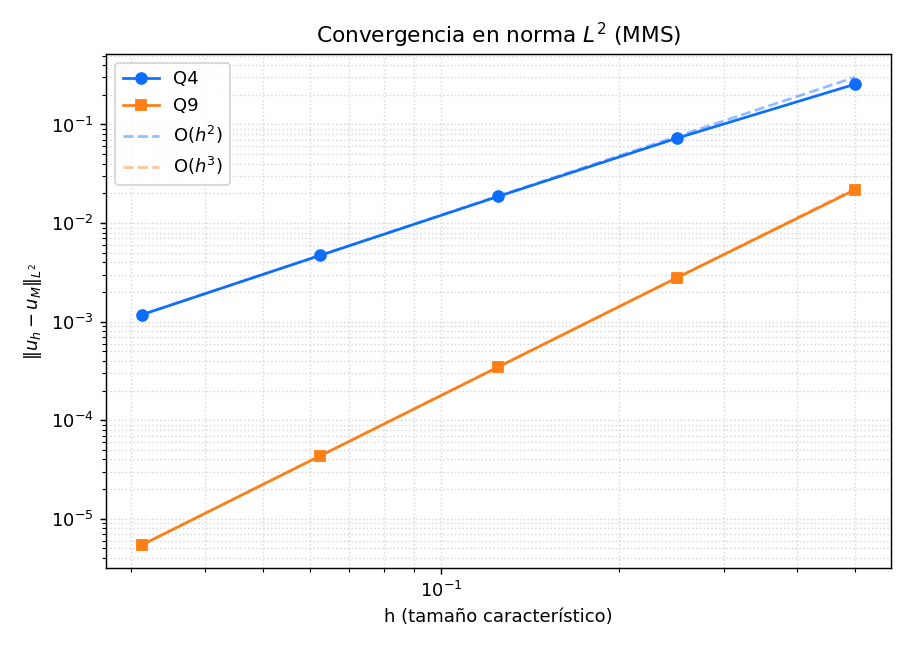
\includegraphics[width=\linewidth]{mms_convergence_l2.png}\\[2pt]
  {\small (a) Norma $L^2$ del desplazamiento.}
\end{minipage}
\hfill
\begin{minipage}{0.49\linewidth}
  \centering
  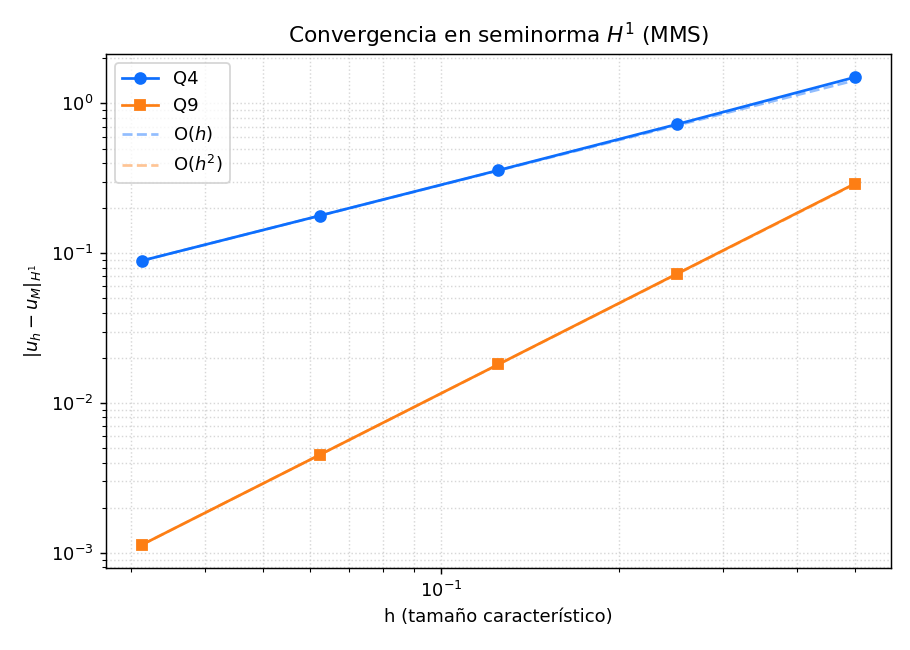
\includegraphics[width=\linewidth]{mms_convergence_h1.png}\\[2pt]
  {\small (b) Seminorma $H^1$ del desplazamiento.}
\end{minipage}
\caption[Convergencia bajo refinamiento $h$ medida por MMS.]{Convergencia bajo refinamiento $h$ medida por MMS (configuración base). Las pendientes de las rectas reproducen las tasas teóricas $\mathcal{O}(h^{p+1})$ en $L^2$ y $\mathcal{O}(h^{p})$ en $H^1$; las líneas discontinuas marcan las pendientes de referencia.}
\label{fig:convergencia}
\end{figure}

\begin{figure}[htbp]
\centering
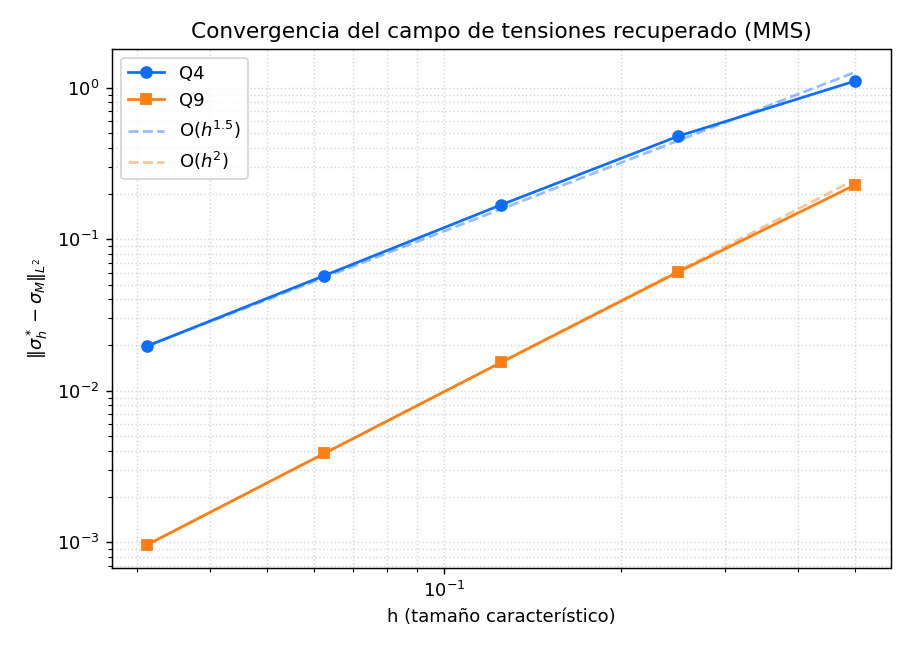
\includegraphics[width=0.62\linewidth]{mms_convergence_stress.png}
\caption[Convergencia del campo de tensiones recuperado medida por MMS.]{Convergencia bajo refinamiento $h$ del campo de tensiones recuperado $\bm{\sigma}^*_h$ (puntos de Gauss $\to$ nodos $\to$ promedio) medida por MMS en la configuración base. Las líneas discontinuas marcan las pendientes de referencia $\mathcal{O}(h^{1{,}5})$ y $\mathcal{O}(h^{2})$, próximas a las tasas asintóticas medidas de 1,54 en el Q4 y 2,00 en el Q9. Las etiquetas de la figura, generadas por el guion, usan el punto decimal.}
\label{fig:convergencia-tension}
\end{figure}

Criterio fijado en la \autoref{sec:validacion-resultados}: la tasa de convergencia del desplazamiento, en las dos normas del error y en las cuatro configuraciones, dentro de $\pm 0{,}5$ de la teórica. Observado: 2,00 en $L^2$ y 1,00 en $H^1$ para el Q4, y 3,00 y 2,00 para el Q9 en la configuración base; en las otras tres, las mismas cifras con diferencias inferiores a 0,01. Se cumple.

\section{Consistencia interna del modelo de datos}
\label{sec:consistencia-interna}

Más allá de la corrección numérica del solucionador, la batería de regresión verifica la robustez de las operaciones de gestión del modelo que distinguen a EduFEM como herramienta interactiva (\autoref{sec:arquitectura}). Tres pruebas resultan especialmente relevantes: el ciclo de transformación entre tipos de elemento, la separación entre identidad del nodo e índice de grado de libertad, y el intercambio de datos con otras herramientas. La tercera sostiene el criterio de intercambio de datos de la cláusula (a) (\autoref{tab:criterios}).

La primera es el ciclo de transformación $\text{Q4}\rightarrow\text{Q9}\rightarrow\text{Q4}$. Al expandir un elemento bilineal a bicuadrático se generan automáticamente cinco nodos adicionales (cuatro nodos medios de arista y el centroide); al reducir de nuevo a Q4 esos nodos auxiliares deben eliminarse sin contaminar el resultado. La prueba comprueba que el campo de desplazamientos calculado sobre la malla Q4 reducida es idéntico al de la malla Q4 original dentro de la tolerancia numérica, con $\max|u_{\text{Q4,inicial}} - u_{\text{Q4,reducido}}| < 10^{-9}$. En este caso, las rutinas de expansión y reducción de malla no introdujeron deriva (\emph{drift}) numérica apreciable.

La segunda prueba aborda la separación entre identidad del nodo e índice de grado de libertad, que la \autoref{sec:identidad-gdl} explica. La prueba resuelve un mismo problema con identificadores no contiguos $\{1,5,50,99\}$ y verifica equivalencia numérica inferior a $10^{-9}$ respecto del mismo problema con identificadores contiguos $\{1,2,3,4\}$. Este resultado es coherente con el patrón de indexación adoptado y, en la configuración ensayada, no reproduce los fallos por indexación directa que aparecían al eliminar nodos.

La tercera prueba verifica el intercambio de datos con otras herramientas que exige el criterio de intercambio de datos de la cláusula (a) (\autoref{tab:criterios}; \texttt{tests/test\_interop.py}). El ejemplo guía exportado al paquete CSV/ZIP y reimportado en un proyecto vacío conserva sus nueve nodos, cuatro elementos, material, cargas y restricciones, y el sistema resuelto sobre el modelo reimportado reproduce los desplazamientos originales con $\max|\Delta u| < 10^{-12}$. El archivo DXF de ejemplo del proyecto —una viga de $4\times1$~m subdividida en seis cuadriláteros en la capa \texttt{FEM\_ELEMENTS}, con una capa decorativa que debe ignorarse— se importa como seis elementos y doce nodos, sin vértices duplicados y en orientación antihoraria, y su reimportación es idempotente: cero nodos y cero elementos nuevos, seis duplicados omitidos. La serialización JSON del formato nativo se verifica por ida y vuelta en \texttt{tests/test\_serialization.py}, y la generación de la memoria de cálculo en PDF, para Q4 y Q9, en \texttt{tests/test\_memoria\_calculo.py}.

Criterio fijado en la \autoref{sec:validacion-resultados}: ida y vuelta CSV sin pérdida, importación DXF repetible y memoria de cálculo generada para Q4 y Q9 sin error. Observado: el modelo reimportado conserva sus nueve nodos y cuatro elementos y reproduce los desplazamientos con $\max|\Delta u| < 10^{-12}$; la reimportación del DXF no creó entidades nuevas —cero nodos y cero elementos, con seis duplicados omitidos—; la memoria se generó para ambos tipos de elemento sin error. Se cumple.

\section{Validación con la viga de Timoshenko}
\label{sec:timoshenko}

La validación confronta el software con una referencia externa de aceptación general. El autor eligió una viga simplemente apoyada de luz $L = 14$~m, peralte $H = 1{,}20$~m y base $b = 0{,}40$~m, sometida a una carga uniforme $q = 5000$~kgf/m. El modelo se planteó en el sistema técnico (kgf, cm), con material $E = 217\,370$~kgf/cm$^2$ (unos $21{,}32$~GPa) y $\nu = 0{,}20$. Ese módulo es el que arroja la correlación módulo--resistencia del hormigón de peso normal, $E = 15\,000\sqrt{f'_c}$ en unidades técnicas, evaluada en $f'_c = 210$~kgf/cm$^2$. El análisis es elástico lineal y no considera la fisuración del hormigón.

El valor concreto de $E$ no condiciona la validación. En elasticidad lineal con cargas prescritas y apoyos de desplazamiento nulo, escalar el módulo por un factor $\alpha$ deja el campo de tensiones inalterado y divide los desplazamientos por $\alpha$. Como las tres soluciones que se comparan ---EduFEM, la solución analítica y el modelo de SAP2000--- usan el mismo módulo, los errores relativos de la \autoref{tab:timoshenko-stress} y de la \autoref{tab:timoshenko-defl} son invariantes ante esa elección. El autor adoptó un hormigón realista únicamente para que las magnitudes del ejemplo resulten familiares al lector de ingeniería civil, no porque de él dependa el resultado.

El autor empleó una única malla Q9 estructurada de $56\times8$ elementos (448 elementos, 1921 nodos, 3842 GDL). Conforme a la \autoref{sec:poblacion}, este caso es un contraste puntual de exactitud sobre una malla fina y no un estudio de convergencia; el refinamiento y la comparación Q4 frente a Q9 se reportan en las secciones del MMS y de la membrana de Cook. Las dos referencias de contraste son la solución analítica de la teoría de la elasticidad de Timoshenko y Goodier \autocite[art.~21, pp.~39-43]{timoshenko1970elasticity} y un modelo equivalente resuelto en SAP2000 con elementos de cáscara (\emph{shell}). En esta viga solo interviene la respuesta de esos elementos en su plano, que sigue una formulación isoparamétrica de membrana con un giro adicional normal al plano (\emph{drilling}) \autocite[p.~179]{csi2017sap2000}. Esa formulación no coincide exactamente con el continuo bidimensional de tensión plana de EduFEM —difiere en la cinemática y en la discretización—, por lo que pequeñas discrepancias entre ambos modelos son esperables y no deben interpretarse como mayor o menor exactitud de uno sobre otro. El detalle del modelo de SAP2000, la resolución analítica de Timoshenko-Goodier y la comparación punto a punto que originan estas referencias se documentan en el \autoref{anexo:sap2000}.

La \autoref{tab:timoshenko-stress} compara la tensión normal $\sigma_x$ en tres puntos de control de la viga —uno en la fibra extrema del centro del vano (A) y dos interiores (B y C)— y, en el punto B, donde su error es máximo, las componentes secundarias $\sigma_y$ y $\tau_{xy}$; el conjunto completo de componentes está en la \autoref{tab:tim-componentes}. Las coordenadas siguen el marco de la solución de Timoshenko-Goodier, con origen en el centro del vano y eje $y$ positivo hacia la fibra traccionada; el guion de validación aplica el cambio de signo $y_{\text{MEF}} = -y_{\text{ref}}$ que documenta el \autoref{anexo:vyv}.

\begin{table}[htbp]
\centering
\caption[Tensiones (kgf/cm$^2$) en los puntos de control de la viga de Timoshenko: EduFEM frente a la solución analítica y a SAP2000.]{Tensiones (kgf/cm$^2$) en los tres puntos de control de la viga de Timoshenko: EduFEM frente a la solución analítica de Timoshenko-Goodier y a SAP2000. Tensión normal $\sigma_x$ en A $(0;\ 0{,}6)$, B $(-4{,}5;\ -0{,}3)$ y C $(-3{,}5;\ -0{,}2)$~m, y componentes secundarias en B, donde su error es máximo.}
\label{tab:timoshenko-stress}
\small
\setlength{\tabcolsep}{4pt}
\begin{tabular}{c l r r r c c}
\hline
Punto & Magnitud & EduFEM & Analítico & SAP2000 & Error anal.\ (\%) & Difer.\ SAP (\%) \\
\hline
A & $\sigma_x$   & $127{,}8825$ & $127{,}8542$ & $127{,}8514$ & 0,02 & 0,02 \\
B & $\sigma_x$   & $-37{,}3410$ & $-37{,}3255$ & $-37{,}2640$ & 0,04 & 0,21 \\
C & $\sigma_x$   & $-31{,}8077$ & $-31{,}7992$ & $-31{,}7852$ & 0,03 & 0,07 \\
B & $\sigma_y$   & $-1{,}0646$  & $-1{,}0547$  & $-1{,}0182$  & 0,94   & 4,56 \\
B & $\tau_{xy}$  & $5{,}4257$   & $5{,}2734$   & $5{,}2818$   & 2,89   & 2,72 \\
\hline
\end{tabular}
{\singlespacing\notaapa{El signo de $\tau_{xy}$ de SAP2000 se lleva a la convención de eje $y$ de la solución analítica (\autoref{anexo:vyv}). La última columna se rotula «diferencia» y no «error» porque la formulación de cáscara de SAP2000 no es la misma que el continuo de tensión plana de EduFEM: ninguna de las dos es patrón de exactitud de la otra.}}
\end{table}

Los errores de $\sigma_x$ frente a la solución analítica permanecen por debajo del $0{,}05\,\%$ en los tres puntos de control, con un máximo de $0{,}04\,\%$ en el punto B; la diferencia frente a SAP2000 alcanza un máximo de $0{,}21\,\%$, también en el punto B. En las componentes secundarias, cuya magnitud es entre seis y treinta y cinco veces menor que la de $\sigma_x$, los porcentajes crecen: en el punto B, el error frente a la solución analítica es del $0{,}94\,\%$ en $\sigma_y$ y del $2{,}89\,\%$ en $\tau_{xy}$, y la diferencia frente a SAP2000, del $4{,}56\,\%$ y del $2{,}72\,\%$. Esas componentes se reportan, pero no forman parte del criterio de aceptación (\autoref{sec:validacion-resultados}); la \autoref{sec:interpretacion} explica por qué crecen. El autor ubicó los puntos A, B y C a distintas alturas y abscisas, en zonas de tracción y de compresión, a lo largo del peralte en el que $\sigma_x$ varía linealmente. Los máximos anteriores se toman sobre esos tres puntos de control y no sobre todos los nodos de la malla: ese máximo sobre el dominio completo no se calculó. La suma de las reacciones verticales en los dos apoyos equilibra la carga total $qL = 70\,000$~kgf con un residuo relativo de $1{,}7\times10^{-13}$, y la suma horizontal no pasa de $4\times10^{-12}$ veces esa carga: ambas quedan en el orden del error de redondeo.

La \autoref{tab:timoshenko-defl} contrasta la deflexión vertical: en el centro de la luz frente a la solución analítica y en los puntos de control frente a SAP2000.

\begin{table}[htbp]
\centering
\caption[Deflexión vertical $|u_y|$ (cm): EduFEM frente a la solución analítica y a SAP2000.]{Deflexión vertical $|u_y|$ (cm) de la viga de Timoshenko: en el centro de la luz frente a la solución analítica con corrección de cortante, y en los tres puntos de control frente a SAP2000.}
\label{tab:timoshenko-defl}
\begin{tabular}{l r r r c c}
\hline
Medición & EduFEM & Analítico & SAP2000 & Error anal.\ (\%) & Difer.\ SAP (\%) \\
\hline
$|u_y|(0;\ 0)$ & $2{,}03460$ & $2{,}02926$ & ---         & 0,26 & --- \\
$|u_y|$ en A & $2{,}03101$ & ---         & $2{,}0231$ & ---    & 0,39 \\
$|u_y|$ en B & $1{,}09871$ & ---         & $1{,}0926$ & ---    & 0,56 \\
$|u_y|$ en C & $1{,}45216$ & ---         & $1{,}4453$ & ---    & 0,47 \\
\hline
\end{tabular}
\end{table}

El error en deflexión es del $0{,}26\,\%$ frente a la solución analítica que incluye la corrección de cortante de Timoshenko \autocite[art.~21, pp.~39-43]{timoshenko1970elasticity}; con la fórmula clásica de Euler-Bernoulli, que desprecia la deformación por cortante, el valor de referencia sería $1{,}9976$~cm y el error aparente del software ascendería al $1{,}85\,\%$. Con una relación luz-peralte de $11{,}7$, la viga es lo bastante esbelta para que la deformación por cortante aporte poco, pero no tanto como para despreciarla: de ahí la distancia entre ese $1{,}85\,\%$ y el $0{,}26\,\%$ que se obtiene frente a la solución con corrección de cortante. Frente a SAP2000, la diferencia en la componente vertical del desplazamiento llega al $0{,}56\,\%$ en el punto B.

La \autoref{fig:timoshenko-contorno} presenta el contorno de tensión normal y la configuración deformada de la viga, que permiten apreciar visualmente la distribución lineal de $\sigma_x$ en el peralte.

\begin{figure}[htbp]
\centering
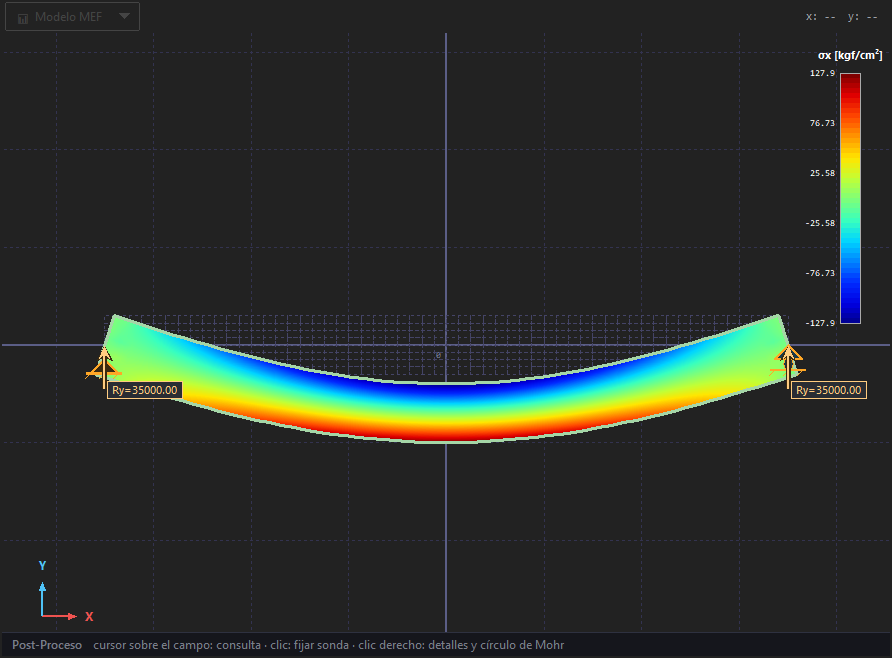
\includegraphics[width=\linewidth]{fig_timoshenko_contorno}
\caption[Campo de $\sigma_x$ sobre la viga de Timoshenko deformada ($56\times8$ Q9).]{Post-proceso de EduFEM: campo de tensión normal $\sigma_x$ sobre la configuración deformada de la viga de Timoshenko ($56\times8$ Q9). La gradación lineal de $\sigma_x$ en el peralte ---tracción (rojo) en la fibra inferior, compresión (azul) en la superior y eje neutro (verde)--- coincide con la predicción de la teoría de vigas. Las etiquetas de la captura conservan el punto decimal del software; las dos reacciones, de 35\,000~kgf, suman la carga total de 70\,000~kgf.}
\label{fig:timoshenko-contorno}
\end{figure}

Criterio fijado en la \autoref{sec:validacion-resultados} para la tensión normal: error de $\sigma_x$ inferior al $1\,\%$ frente a la solución analítica y diferencia inferior al $1\,\%$ frente a SAP2000, en los tres puntos de control. Observado: $0{,}04\,\%$ de error y $0{,}21\,\%$ de diferencia, ambos en el punto B. Se cumple. Criterio para la flecha: error inferior al $3\,\%$ frente a la solución analítica. Observado: $0{,}26\,\%$ en el centro de la luz. Se cumple. Criterio para el equilibrio: residuo relativo de la suma de reacciones inferior a $10^{-8}$. Observado: $1{,}7\times10^{-13}$. Se cumple.

\section{Validación con la membrana de Cook y el bloqueo por cortante}
\label{sec:cook}

La membrana de Cook es un caso de estudio clásico de la literatura de elementos finitos, que debe su nombre a R. D. Cook \autocite[p.~27]{stembera2019dkmq24} y resulta especialmente sensible al bloqueo por cortante (\emph{shear locking}) por combinar flexión, cortante y distorsión geométrica en un cuadrilátero trapezoidal. El dominio es un trapecio de vértices $(0;\ 0)$, $(48;\ 44)$, $(48;\ 60)$ y $(0;\ 44)$, empotrado en el borde izquierdo y cargado con una fuerza tangencial total unitaria en el borde derecho; el material es adimensional con $E = 1{,}0$, $\nu = 1/3$ y $t = 1{,}0$ en tensión plana. La cantidad de interés es el desplazamiento vertical $u_y$ en el punto $(48;\ 52)$, para la que el autor adoptó el valor de referencia $u_y^{\mathrm{ref}} = 23{,}96$, de uso extendido para este caso. El planteamiento reproduce el de la literatura reciente, que emplea la misma geometría, el mismo material y la misma carga tangencial unitaria \autocite[p.~27]{stembera2019dkmq24}.

Ese valor de referencia merece una precisión, porque es el único de los tres casos que no procede de una solución analítica cerrada: es un límite de convergencia y no un dato exacto. La literatura no lo trata de otro modo: Štembera y Füssl, que lo emplean para ensayar el comportamiento de membrana de un elemento de cáscara, advierten que este problema no tiene solución analítica disponible y obtienen su referencia por vía numérica, con una malla de $192\times128$ elementos, en $23{,}965$ \autocite[p.~28]{stembera2019dkmq24}. Este trabajo lo corrobora además con evidencia propia. La secuencia Q9 ($23{,}925 \to 23{,}949 \to 23{,}961$) todavía se mueve en la malla más fina, y su extrapolación de Richardson \autocite[pp.~309-312]{oberkampf2010vv} apunta a $\approx 23{,}97$, consistente con el valor adoptado; el orden observado, próximo a uno, refleja la singularidad de tensiones en los dos vértices del borde empotrado, donde la restricción cambia bruscamente de desplazamiento impuesto a borde libre. La incertidumbre de la referencia es, por tanto, del orden del $0{,}05\,\%$: es lo que separa las dos mallas Q9 más finas, $(23{,}961-23{,}949)/23{,}96$, y es del mismo orden que la distancia, del $0{,}04\,\%$, entre $23{,}96$ y el $23{,}97$ de la extrapolación. El valor publicado, $23{,}965$, cae dentro de ese intervalo, lo que respalda a la vez la referencia adoptada y la incertidumbre estimada. Los errores por debajo del $0{,}1\,\%$ ---el doble de esa incertidumbre--- no se distinguen de ella y no deben leerse como exactitud del elemento.

La \autoref{tab:cook} reúne la convergencia bajo refinamiento $N$ para ambos elementos.

\begin{table}[htbp]
\centering
\caption[Convergencia del desplazamiento $u_y$ en $(48;\ 52)$ para la membrana de Cook.]{Convergencia del desplazamiento $u_y$ en $(48;\ 52)$ para la membrana de Cook, bajo refinamiento $N$, con los elementos Q4 y Q9. Referencia adoptada $u_y^{\mathrm{ref}} = 23{,}96$, con una incertidumbre del orden del $0{,}05\,\%$; el error se mide respecto de ella. La fuente publicada da $23{,}965$ para esa misma cantidad \autocite[p.~28]{stembera2019dkmq24}.}
\label{tab:cook}
\begin{tabular}{c r r r r r r}
\hline
 & \multicolumn{3}{c}{\textbf{Q4}} & \multicolumn{3}{c}{\textbf{Q9}} \\
$N$ & GDL & $u_y$ & error (\%) & GDL & $u_y$ & error (\%) \\
\hline
2  & 18   & $11{,}845$ & $-50{,}563$ & 50   & $23{,}289$ & $-2{,}802$ \\
4  & 50   & $18{,}299$ & $-23{,}626$ & 162  & $23{,}840$ & $-0{,}502$ \\
8  & 162  & $22{,}079$ & $-7{,}850$  & 578  & $23{,}925$ & $-0{,}144$ \\
16 & 578  & $23{,}430$ & $-2{,}210$  & 2178 & $23{,}949$ & $-0{,}044$ \\
32 & 2178 & $23{,}818$ & $-0{,}594$  & 8450 & $23{,}961$ & $+0{,}003$ \\
\hline
\end{tabular}
\end{table}

El elemento Q4 subestima la respuesta en más de un $50\,\%$ en la malla más gruesa y conserva un error del $-0{,}594\,\%$ con $N=32$ (2178 GDL); su convergencia es lenta y monótona por debajo de la referencia. El elemento Q9 alcanza un error del $-0{,}144\,\%$ con $N=8$ (578 GDL) y del $-0{,}044\,\%$ con $N=16$ (2178 GDL), este último ya dentro de la incertidumbre de la propia referencia. Con 578 GDL ---que el Q4 alcanza con $N=16$ y el Q9 con $N=8$--- el error del Q9 es más de diez veces menor que el del Q4: poco más de quince veces con el $23{,}96$ adoptado, más de trece con el $23{,}965$ publicado y doce con el $23{,}97$ de la extrapolación. Con 2178 GDL la razón deja de ser informativa: el error del Q9 cae por debajo del $0{,}1\,\%$ y ya no se distingue de la incertidumbre de la referencia. La flecha del Q4 es menor que la del Q9 en las cinco mallas ensayadas, que es la firma del bloqueo por cortante.

Esa secuencia admite además un contraste externo directo, que es lo que distingue a este caso de una comprobación puramente interna. Štembera y Füssl publican, para el mismo problema y el mismo refinamiento, los desplazamientos que obtienen con un cuadrilátero de cuatro nodos: $11{,}845$, $18{,}299$, $22{,}079$, $23{,}430$ y $23{,}818$ \autocite[p.~28]{stembera2019dkmq24}. Son, en las cinco mallas y hasta la última cifra publicada, los mismos valores que EduFEM calcula con su elemento Q4 (\autoref{tab:cook}). La coincidencia no prueba que ambos programas sean correctos, porque un error compartido de formulación se reproduciría en los dos; sí muestra que el motor de EduFEM resuelve este caso como lo resuelve un código independiente, desarrollado por otros autores y publicado.

La \autoref{fig:cook-convergencia} muestra las curvas de convergencia de $u_y$ frente al número de grados de libertad para ambos elementos.

\begin{figure}[htbp]
\centering
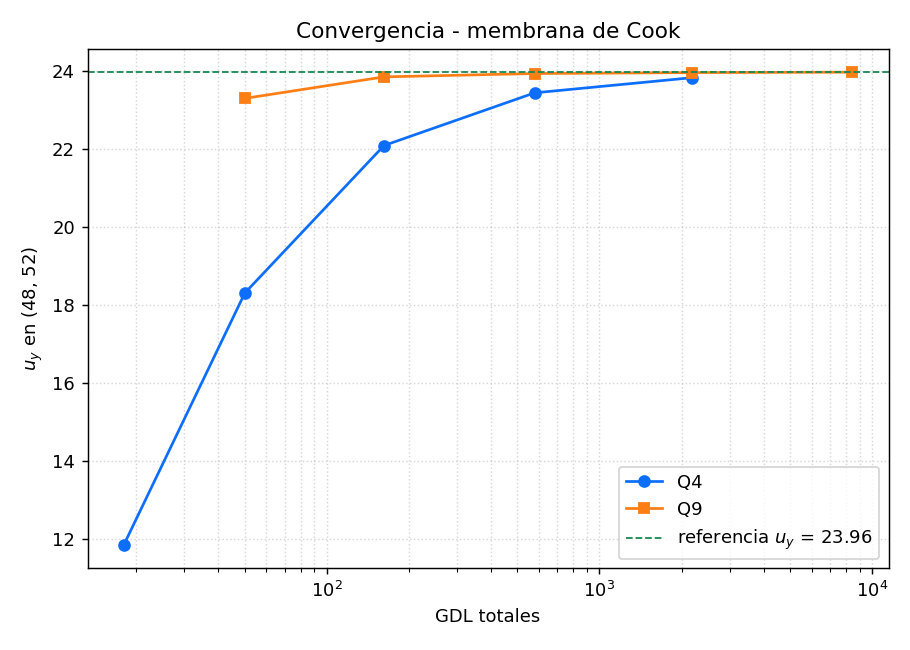
\includegraphics[width=0.72\linewidth]{cook_convergence.png}
\caption[Convergencia del desplazamiento $u_y$ de la membrana de Cook para Q4 y Q9.]{Convergencia del desplazamiento vertical $u_y$ en $(48;\ 52)$ de la membrana de Cook para los elementos Q4 y Q9, frente al número de grados de libertad en escala logarítmica. La línea horizontal discontinua marca el valor de referencia adoptado, $u_y^{\mathrm{ref}} = 23{,}96$. Las etiquetas de la figura, generadas por el guion, usan el punto decimal.}
\label{fig:cook-convergencia}
\end{figure}

Criterio fijado en la \autoref{sec:validacion-resultados} para la exactitud: error del desplazamiento con Q9 y $N=8$ inferior al $1{,}5\,\%$ en valor absoluto. Observado: $-0{,}144\,\%$, es decir, $0{,}144\,\%$ en valor absoluto. Se cumple. Criterio para el bloqueo por cortante: flecha del Q4 menor que la del Q9 con la misma malla. Observado: así ocurre en las cinco mallas. Se cumple.

La \autoref{tab:resumen-q4q9} sintetiza la comparación global entre ambos elementos a lo largo de las tres baterías de prueba.

\begin{table}[htbp]
\centering
\caption[Síntesis comparativa Q4 frente a Q9 en las baterías de verificación y validación.]{Síntesis comparativa Q4 frente a Q9 en las baterías de verificación y validación: tasas asintóticas de convergencia del desplazamiento medidas por MMS, desplazamiento $u_y$ y su error en la membrana de Cook a igualdad de refinamiento, y error de $\sigma_x$ en la viga de Timoshenko; la última fila resume en palabras el comportamiento de cada elemento bajo distorsión.}
\label{tab:resumen-q4q9}
\begin{tabular}{l c c}
\hline
Aspecto & Q4 (bilineal) & Q9 (bicuadrático) \\
\hline
Tasa $L^2$ (MMS)              & $\mathcal{O}(h^{2{,}00})$ & $\mathcal{O}(h^{3{,}00})$ \\
Tasa $H^1$ (MMS)              & $\mathcal{O}(h^{1{,}00})$ & $\mathcal{O}(h^{2{,}00})$ \\
Cook $N=8$ (162 / 578 GDL)    & $22{,}079$ ($-7{,}850\,\%$) & $23{,}925$ ($-0{,}144\,\%$) \\
Cook $N=16$ (578 / 2178 GDL)  & $23{,}430$ ($-2{,}210\,\%$) & $23{,}949$ ($-0{,}044\,\%$) \\
Timoshenko $\sigma_x$ (máx.\ en A, B y C) & --- & $0{,}04\,\%$ \\
Comportamiento bajo distorsión & bloqueo parcial & sin bloqueo apreciable \\
\hline
\end{tabular}
{\singlespacing\notaapa{La viga de Timoshenko se resolvió únicamente con Q9 (\autoref{sec:poblacion}). Su error de $\sigma_x$ es el máximo entre los tres puntos de control A, B y C de la \autoref{tab:timoshenko-stress}, frente a la solución analítica; el máximo sobre todos los nodos de la malla no se calculó.}}
\end{table}

\section{Cobertura del procedimiento y del contenido}
\label{sec:cobertura}

Esta sección reporta la cláusula (a) de la hipótesis, la trazabilidad. Primero, qué expone el software y cómo; después, si lo expuesto cubre el contenido que los expertos exigen. Cierra con la procedencia de cada decisión sobre cómo exponerlo, que es la evidencia de la condición de la hipótesis: el método de diseño aplicado.

\subsection{Cobertura del procedimiento y organización de la interfaz}
\label{sec:cobertura-canal}

La \autoref{tab:fases} resume qué operaciones ofrece cada fase del análisis, qué etapas del procedimiento de cálculo expone y con qué instrumento; la \autoref{fig:fases-lienzo} muestra las tres fases operando sobre el mismo lienzo y el mismo modelo.

\begin{table}[!htbp]
\centering
\caption[Fases del análisis en EduFEM: operaciones y exposición del procedimiento.]{Fases del análisis en EduFEM. Por cada fase: las operaciones disponibles, las etapas del procedimiento de cálculo que expone y el instrumento con que lo hace. Las nueve etapas son las enumeradas en la \autoref{sec:variables-met}; la discretización y la calidad de malla las anteceden y no se cuentan entre ellas.}
\label{tab:fases}
{\footnotesize
\setlength{\tabcolsep}{4pt}
\begin{tabular}{@{}>{\raggedright\arraybackslash}p{1.9cm}>{\raggedright\arraybackslash}p{5.1cm}>{\raggedright\arraybackslash}p{3.3cm}>{\raggedright\arraybackslash}p{3.7cm}@{}}
\toprule
\textbf{Fase} & \textbf{Operaciones disponibles} & \textbf{Etapas que expone} & \textbf{Instrumento de exposición} \\
\midrule
Pre-proceso & Definición tabular y gráfica de nodos, elementos, cargas y restricciones; diálogo de materiales; importación DXF; deshacer y rehacer; comprobador de salud & Discretización y calidad de malla & M0 (calidad de malla, coloreado por elemento y distorsión en vivo) \\
Proceso & Resolución del sistema con comprobación previa; exploración del procedimiento sobre el elemento seleccionado en el lienzo & Mapeo isoparamétrico, $\bm{J}$, $\bm{B}$, $\bm{D}$, $\bm{k}_e$ por cuadratura, fuerzas nodales equivalentes, ensamblaje (etapas 1 a 7) & M1 a M7: capas superpuestas; conmutador Fórmula~$\leftrightarrow$~Valores en M2, M3 y M4 \\
Post-proceso & Contornos de tensión y desplazamiento, deformada, isolíneas, vista tridimensional, sonda puntual con círculo de Mohr, reacciones, tabla de resultados, exportación de la memoria & Solución del sistema y recuperación de tensiones, en modo crudo y suavizado (etapas 8 y 9) & Sonda, vista tridimensional y tabla de resultados; memoria de cálculo (las nueve etapas, con sustitución numérica) \\
\bottomrule
\end{tabular}}
\end{table}

\begin{figure}[p]
\centering
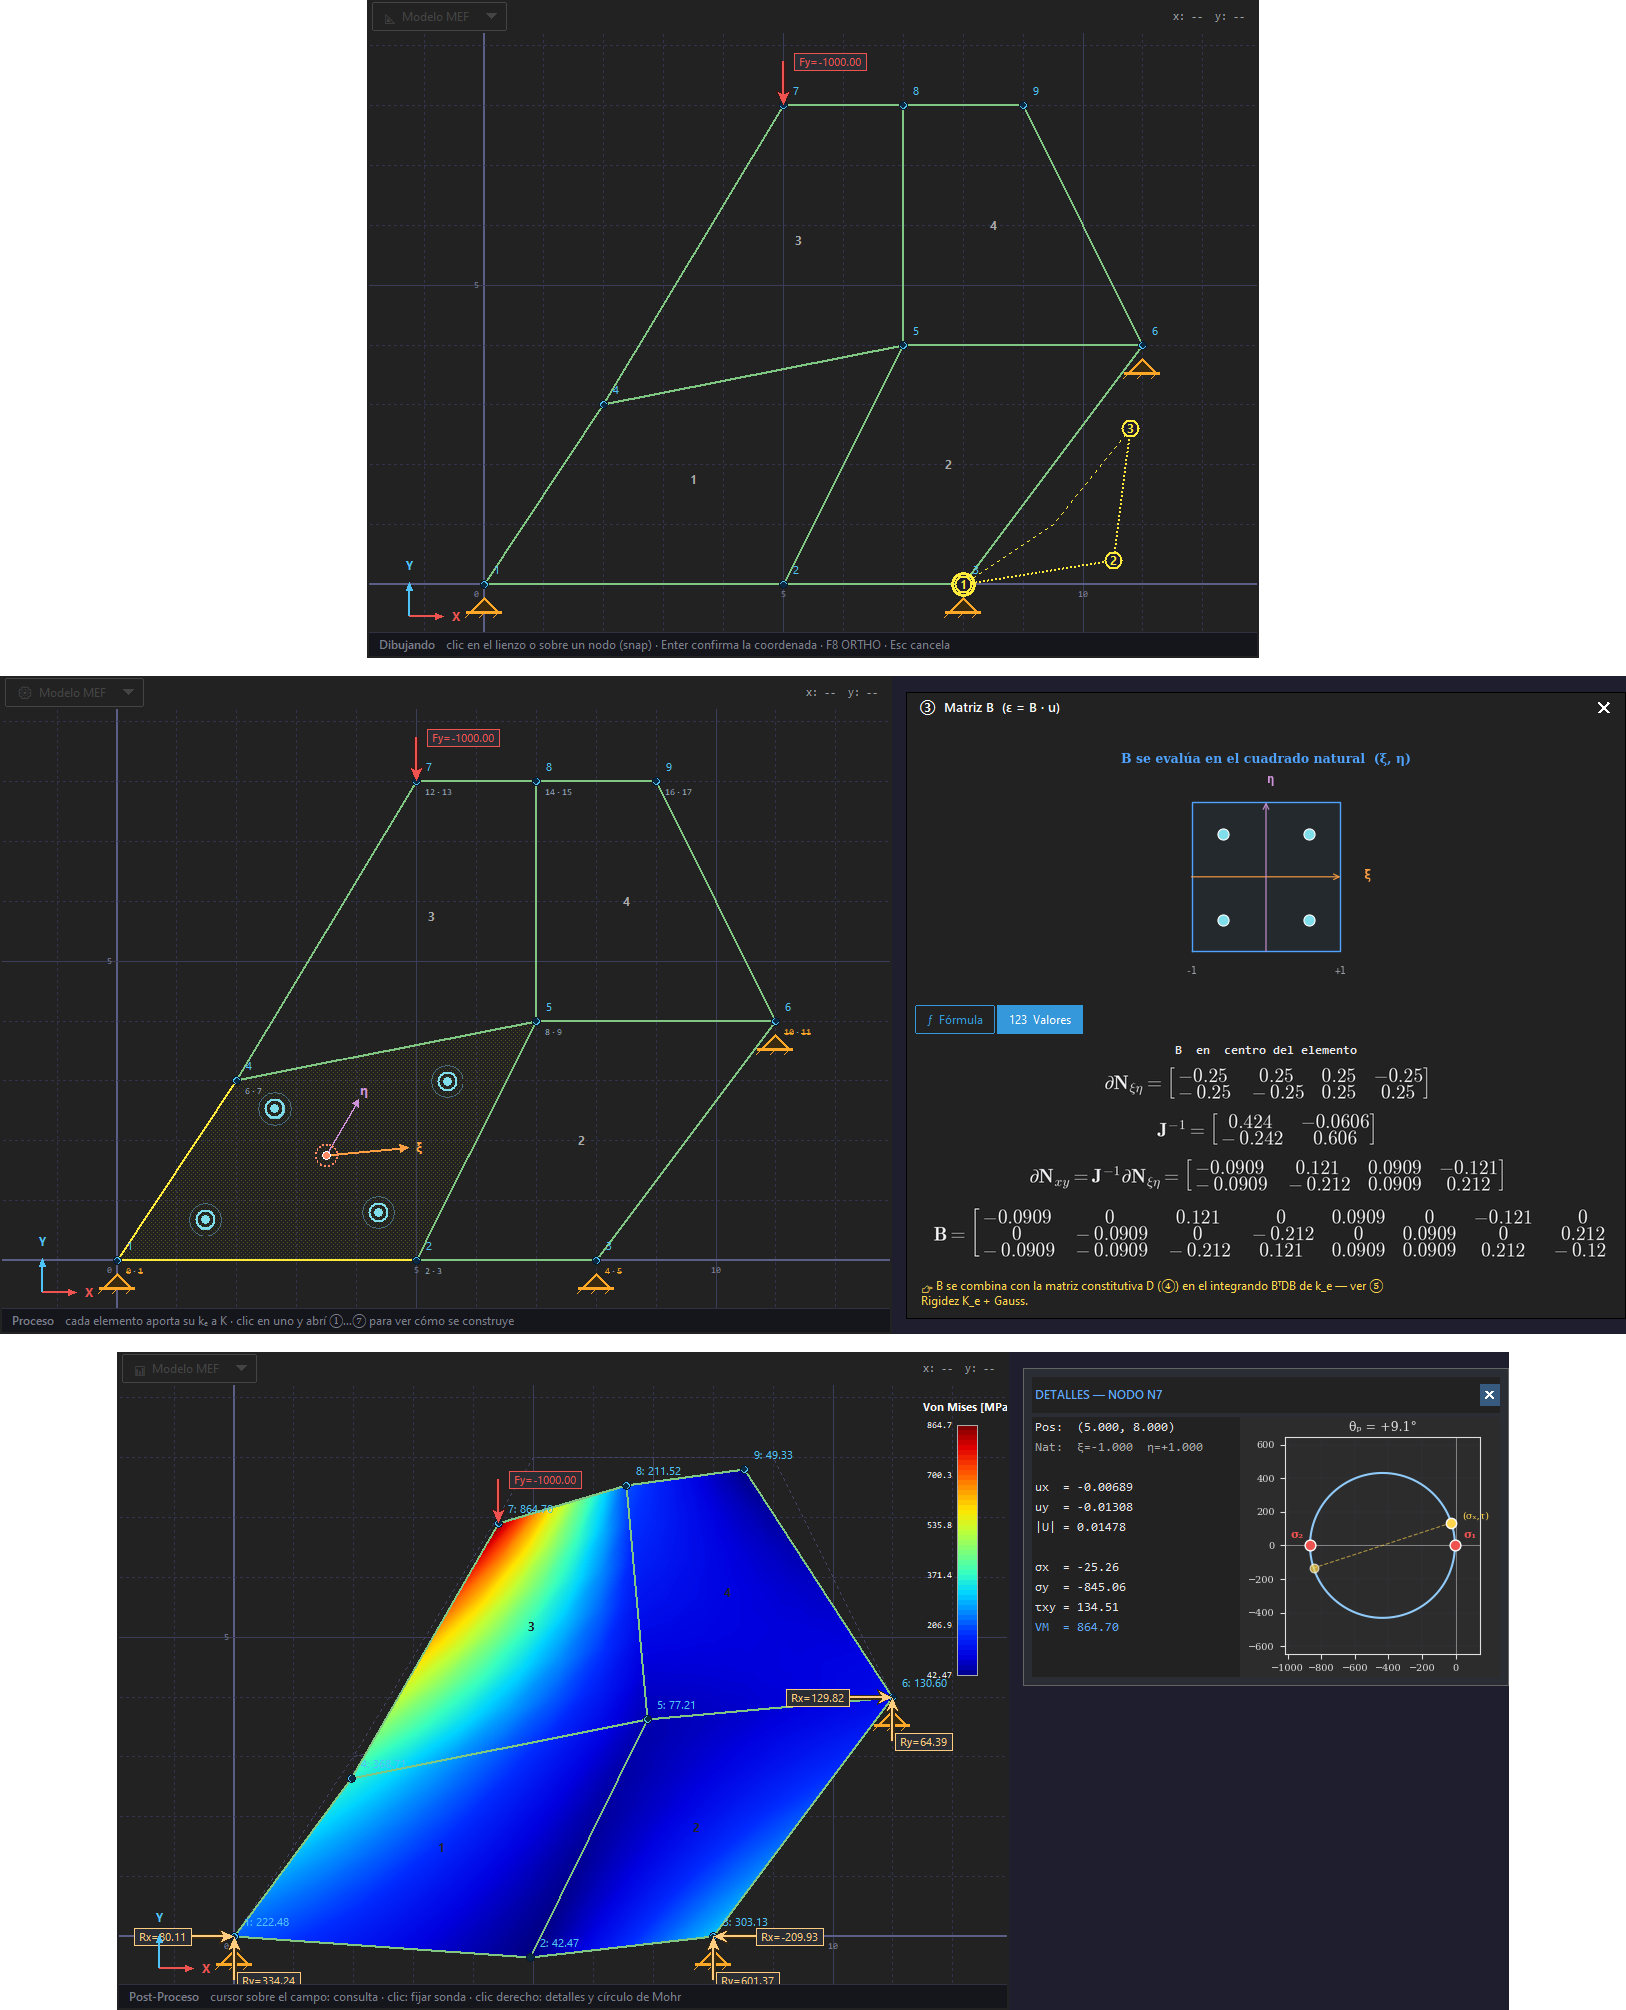
\includegraphics[width=0.95\linewidth]{fig_fases_lienzo}
\caption[Las tres fases del análisis sobre el mismo lienzo y el mismo modelo.]{Las tres fases del análisis sobre el mismo lienzo y el mismo modelo (ejemplo guía: nueve nodos, cuatro elementos Q4, carga en el nodo 7). De arriba abajo: pre-proceso, con el modo de dibujo agregando un elemento sobre la malla existente; proceso, con el módulo M3 desplegado sobre el elemento seleccionado y los índices de grado de libertad junto a cada nodo; post-proceso, con el contorno de von Mises sobre la deformada, las reacciones en los apoyos y el panel de detalles del nodo 7 con su círculo de Mohr. Capturas de EduFEM; a tamaño completo, en la \autoref{fig:lienzo-lod}, la \autoref{fig:modulo-capa} y la \autoref{fig:post-proceso}.}
\label{fig:fases-lienzo}
\end{figure}

\paragraph{Cobertura del procedimiento} De las nueve etapas enumeradas en la \autoref{sec:variables-met}, las siete primeras tienen módulo educativo propio (M1 a M7, \autoref{tab:modulos}) y las nueve tienen desarrollo con sustitución numérica en la memoria de cálculo (\autoref{anexo:memoria}). La solución del sistema y la recuperación de tensiones —las etapas 8 y 9, que no tienen módulo propio— se exponen además en el post-proceso, mediante la sonda puntual con sus modos crudo y suavizado, la vista tridimensional y la tabla de resultados. El módulo M0 atiende la calidad de malla en el pre-proceso, con los mínimos de la biblioteca Verdict \autocite[pp.~51, 57]{stimpson2007verdict}, el del Jacobiano escalado endurecido según la \autoref{sec:pre-proceso}.

Criterios fijados en la \autoref{sec:validacion-resultados}: siete de siete etapas con módulo educativo, y nueve de nueve con desarrollo en la memoria. Observado: 7 de 7 y 9 de 9. Se cumplen. Criterio: solución y tensiones expuestas en el post-proceso, en modo crudo y suavizado. Observado: ambas, con los dos modos. Se cumple.

Los módulos M1 a M7 recorren la fase de proceso en el orden del método, que refleja la dependencia lógica entre conceptos: la secuencia cinemática $\bm{N}\rightarrow\bm{J}\rightarrow\bm{B}$ precede a la constitutiva, y la deformación $\bm{\varepsilon} = \bm{B}\,\bm{u}$ antecede a la tensión $\bm{\sigma} = \bm{D}\,\bm{\varepsilon}$. Es el orden con que la literatura de referencia presenta la formulación isoparamétrica \autocites[pp.~339-347]{bathe2014fem}{cook2002concepts}, y es el que el autor adoptó para los módulos antes de construirlos; el criterio de la \autoref{sec:validacion-resultados} verifica que cada una de las siete etapas tenga módulo, no el orden en que se recorren. Cada módulo es una capa superpuesta sobre la malla real, con la disposición que describe la \autoref{sec:educacion}.

\paragraph{Organización de la interfaz} Las tres fases operan sobre un único lienzo compartido. En la viga de Timoshenko, en la membrana de Cook y en el ejemplo guía, el modelo se construyó o se importó, se resolvió y se inspeccionó sin cambiar de vista, y la selección de un elemento en la tabla o en el lienzo se reflejó en el otro. El caso de soluciones manufacturadas se resolvió solo con su guion, porque su fuerza de volumen es una función del punto y sus desplazamientos impuestos no son nulos, dos datos que la interfaz no admite. Criterio: las tres fases sobre el mismo lienzo. Observado: 3 de 3 fases, en los casos que la interfaz admite. Se cumple.

\paragraph{Trazabilidad e intercambio de datos} La memoria de cálculo se generó para el ejemplo guía en Q4 y en Q9 sin error de compilación (\mbox{\texttt{tests/test\_memoria\_calculo.py}}); el \autoref{anexo:memoria} reproduce su secuencia de sustitución numérica, con cada paso remitido a la ecuación del \autoref{cap:marco_teorico} de la que procede, para que pueda rehacerse con lápiz y papel o en una hoja de cálculo. Cada valor que la memoria muestra coincide con el que calcula el motor: la memoria lo recalcula con la versión legible del motor, y la prueba de regresión la mantiene coincidente con la que resuelve (\autoref{sec:motor}). La ida y vuelta CSV y la repetibilidad de la importación DXF se reportaron en la \autoref{sec:consistencia-interna}. Ese resultado tiene un alcance acotado: lo comprobado es que el paquete CSV transporta sin pérdida las entidades del modelo ensayado —nodos, elementos, material, cargas y restricciones—, no que sea equivalente al formato nativo, que guarda además el valor de los desplazamientos prescritos y la configuración del proyecto. El formato de intercambio está pensado para editar un modelo en una hoja de cálculo, y ese alcance es el que la prueba cubre; el veredicto de ese criterio se da en la \autoref{sec:consistencia-interna}.

\subsection{Cobertura de contenido}
\label{sec:contenido-didactico}

La \autoref{tab:especificaciones} cruza el universo de contenido de la \autoref{sec:poblacion} —las quince destrezas y los tres conceptos que el consenso de expertos de Pérez-Santiago y Campos califica como necesarios para el egresado \autocite[pp.~1162-1163]{perezsantiago2023fem}— con el instrumento de EduFEM que cubre cada uno y con la evidencia de este documento que lo respalda. Los códigos de la primera columna son los del propio consenso: FEA para las destrezas prácticas y FEM para los conceptos teóricos. La regla de marcado es la de la \autoref{sec:validacion-datos}: un ítem se da por cubierto solo si el instrumento existe en la versión evaluada y el documento lo describe.

{\footnotesize
\setlength{\tabcolsep}{3pt}
\renewcommand{\arraystretch}{1.12}
\begin{longtable}{@{}>{\raggedright\arraybackslash}p{1.3cm}>{\raggedright\arraybackslash}p{5.3cm}>{\raggedright\arraybackslash}p{5.2cm}>{\raggedright\arraybackslash}p{2.6cm}@{}}
\caption[Tabla de cobertura de contenido: destrezas y conceptos exigidos por los expertos e instrumento de EduFEM que los cubre.]{Tabla de cobertura de contenido. Por cada destreza o concepto que el consenso de expertos exige al egresado, dentro del alcance de este trabajo: el instrumento de EduFEM que lo cubre y la evidencia que lo respalda en este documento.}\label{tab:especificaciones}\\
\toprule
\textbf{Ítem} & \textbf{Destreza o concepto} & \textbf{Instrumento de EduFEM} & \textbf{Evidencia} \\
\midrule
\endfirsthead
\caption[]{Tabla de cobertura de contenido (continuación).}\\
\toprule
\textbf{Ítem} & \textbf{Destreza o concepto} & \textbf{Instrumento de EduFEM} & \textbf{Evidencia} \\
\midrule
\endhead
\bottomrule
\endfoot
\multicolumn{4}{@{}l}{\textbf{Mallado}} \\
FEA13 & Selección del tipo de elemento & Conversión Q4~$\leftrightarrow$~Q9 del modelo & \autoref{anexo:manual}; \autoref{sec:cook} \\
FEA14 & Definición del tamaño de elemento & Refinamiento manual; secuencias de malla de 2 a 32 elementos por lado & \autoref{tab:mms}; \autoref{tab:cook} \\
FEA15 & Efecto de la relación de aspecto y la distorsión en la exactitud & M0 (calidad en vivo); M2 ($\det\bm{J}$); soluciones manufacturadas sobre malla distorsionada & \autoref{sec:educacion}; \autoref{tab:mms-configs} \\
FEA16 & Efecto del orden del elemento en la exactitud & Cook: Q4 frente a Q9 a igual número de grados de libertad & \autoref{tab:cook}; \autoref{tab:resumen-q4q9} \\
FEA17 & Refinamiento y convergencia de la malla & Tasas de convergencia; curvas de error & \autoref{tab:mms}; \autoref{fig:convergencia} \\
FEA18 & Refinar en zonas de concentración de tensiones & Construcción de la malla con densidad variable, por tabla o sobre el lienzo, con la calidad de cada elemento a la vista en M0; la membrana de Cook concentra tensiones en los vértices del borde empotrado & \autoref{sec:pre-proceso}; \autoref{sec:cook} \\
\multicolumn{4}{@{}l}{\textbf{Post-proceso}} \\
FEA26 & Presentar resultados de desplazamiento y tensión & Contornos, isolíneas, vista tridimensional, tabla de resultados & \autoref{sec:post-proceso}; \autoref{fig:fases-lienzo} \\
FEA27 & Diferencia entre tensiones nodales y elementales & Sonda y vista tridimensional en modo crudo y suavizado & \autoref{sec:post-proceso}; \autoref{tab:fases} \\
FEA28 & Deformada escalada & Deformada con factor de escala configurable & \autoref{sec:post-proceso} \\
\multicolumn{4}{@{}l}{\textbf{Conceptos fundamentales}} \\
FEA29 & Visualizar el efecto de las cargas y compararlo con los resultados & Lienzo único: cargas del pre-proceso y campos del post-proceso sobre el mismo modelo & \autoref{fig:fases-lienzo} \\
FEA30 & Prueba de convergencia refinando hasta una diferencia dada & Secuencias de malla con la diferencia entre mallas sucesivas como regla de parada, y extrapolación de Richardson para estimar el límite & \autoref{tab:mms}; \autoref{sec:cook} \\
FEA31 & Definición de la tensión de von Mises & Contorno y sonda de von Mises; círculo de Mohr & \autoref{sec:post-proceso} \\
\multicolumn{4}{@{}l}{\textbf{Verificación y validación}} \\
FEA32 & Revisar las tensiones para decidir el refinamiento & Modo crudo frente a suavizado; diagnóstico de la memoria & \autoref{sec:post-proceso}; \autoref{sec:memoria-io} \\
FEA33 & Comparar las reacciones con las cargas aplicadas & Reacciones en el post-proceso; comprobación de equilibrio en la memoria & \autoref{sec:timoshenko}; \autoref{sec:memoria-io} \\
FEA34 & Correlacionar los resultados con referencias externas & Contraste con la solución analítica y con SAP2000 & \autoref{sec:timoshenko} \\
\multicolumn{4}{@{}l}{\textbf{Conceptos teóricos del procedimiento}} \\
FEM2 & Ensamblar las rigideces elementales, aplicar restricciones y resolver & M7; memoria (ensamblaje y solución) & \autoref{sec:educacion}; \autoref{anexo:memoria} \\
FEM8 & Formulación isoparamétrica de elementos bidimensionales & M1, M2 y M3 & \autoref{tab:modulos} \\
FEM9 & Integración numérica de Gauss para evaluar tensiones en cualquier punto & M5 (puntos de Gauss variables); sonda del post-proceso & \autoref{sec:educacion}; \autoref{sec:post-proceso} \\
\end{longtable}}
{\singlespacing\notaapa{Códigos e ítems según las tablas 1 y 2 del consenso de expertos \autocite[pp.~1162-1163]{perezsantiago2023fem}, traducidos por el autor. De los 49 ítems de contenido del consenso, estos 18 forman el universo y los 31 restantes quedan fuera por tres motivos; la procedencia del universo y el alcance de la advertencia de generalización de la fuente se discuten en la \autoref{sec:validacion-datos}. Fuera del alcance disciplinar de EduFEM (18): resortes, barras y vigas (FEM1, FEM4, FEM5), elementos axisimétricos (FEM6, FEM7), análisis tridimensional (FEM10--FEM13), placas y cáscaras (FEM14), problemas térmicos (FEM15), modelado e idealización en CAD (FEA6--FEA9), cargas tomadas de un análisis previo (FEA21), elementos rígidos (FEA22) y contacto (FEA23). Anteriores al procedimiento de cálculo, por pertenecer a la planificación del análisis, a la selección de materiales o al modelado de cargas y apoyos (12): FEA1--FEA5, FEA10--FEA12, FEA19, FEA20, FEA24 y FEA25. No expuesto por el software (1): la deducción de la matriz de rigidez por métodos alternativos (FEM3), que es un desarrollo teórico. Los siete ítems de tipo de análisis (TYPE1--TYPE7) y los quince de herramientas de cómputo (SW1--SW15) no forman parte de esos 49: el consenso los trata en categorías aparte, y quedan fuera porque EduFEM resuelve solo el caso estático lineal y porque los segundos valoran programas concretos, no contenidos del procedimiento.}}

El autor cotejó, ítem por ítem y con la regla de marcado de la \autoref{sec:validacion-datos}, que las quince destrezas y los tres conceptos tienen instrumento identificable en la versión evaluada. Criterio fijado en la \autoref{sec:validacion-resultados}: los 18 ítems con instrumento. Observado: 18 de 18. Se cumple.

Ese resultado respalda cobertura y trazabilidad: que para cada contenido exigido existe en el software un instrumento identificable, y que ese instrumento está descrito en este documento. No respalda suficiencia ni profundidad —no dice cuánto cubre cada instrumento— ni efecto sobre quien lo usa. Dos filas piden una precisión, porque su instrumento no es una función que el software ejecute por sí sola. El refinamiento local de FEA18 se obtiene construyendo la malla con más elementos donde se los necesita, no con un algoritmo adaptativo: la herramienta no incorpora mallado automático, como declara la Introducción (\emph{Alcance y limitaciones}). Y la regla de parada de FEA30 la aplica quien compara dos mallas sucesivas, con la diferencia que la \autoref{tab:cook} deja a la vista. En ambos casos el instrumento existe y está descrito, pero lo ejecuta el usuario sobre el modelo. La cobertura tampoco es uniforme: las destrezas de mallado y de verificación se apoyan sobre todo en los casos de estudio y en la memoria, es decir, en lo que el usuario hace con la herramienta sobre un modelo, mientras que las de post-proceso y los conceptos del procedimiento tienen un instrumento propio de la interfaz. Ninguna se cubre solo con texto.

\subsection{Procedencia de las decisiones de diseño}
\label{sec:trazabilidad-diseno}

La \autoref{tab:principios} documenta la condición de la hipótesis: que el desarrollo siguió un método de diseño de software educativo (\autoref{sec:proceso-met}). No registra qué expone el software, sino de dónde procede cada decisión sobre cómo exponerlo. Para cada uno de los cuatro principios de la \autoref{sec:fundamentos-pedagogicos}, registra la decisión de diseño que lo concreta y la evidencia comprobable en el software distribuido.

\begin{table}[htbp]
\centering
\caption[Principios, decisiones de diseño y evidencia.]{Procedencia de las decisiones de diseño. Por cada principio de la \autoref{sec:fundamentos-pedagogicos}: la decisión de diseño de EduFEM que lo concreta y la evidencia comprobable en el software distribuido. La tabla la construyó el autor.}
\label{tab:principios}
{\footnotesize
\setlength{\tabcolsep}{3pt}
\renewcommand{\arraystretch}{1.12}
\begin{tabular}{@{}>{\raggedright\arraybackslash}p{3.4cm}>{\raggedright\arraybackslash}p{5.6cm}>{\raggedright\arraybackslash}p{5.4cm}@{}}
\toprule
\textbf{Principio (fuentes)} & \textbf{Decisión de diseño en EduFEM} & \textbf{Evidencia comprobable} \\
\midrule
Visibilidad del procedimiento \autocite[p.~157]{lee2015interactive} & Módulos M1 a M7 que exponen cada matriz sobre el elemento seleccionado, con la versión legible del motor; memoria con sustitución numérica de las nueve etapas; respuesta expuesta junto con su procedimiento & Siete de siete etapas con módulo y nueve de nueve en la memoria (\autoref{sec:cobertura-canal}); generación de la memoria para Q4 y Q9 en la batería de regresión \\
Interactividad con vínculo al modelo \autocite[pp.~163, 166]{lee2015interactive} & Capa superpuesta que ilumina sobre la malla real el punto del cálculo; conmutador fórmula--valores; selección sincronizada entre lienzo y tabla; conversión Q4~$\leftrightarrow$~Q9 y refinamiento; sonda en modo crudo y suavizado & \autoref{fig:modulo-capa}; \autoref{fig:fases-lienzo}; \autoref{sec:pre-proceso}; \autoref{tab:cook} \\
Construcción paso a paso \autocite[pp.~1010-1011, 1023]{bishay2020teaching} & Un módulo por etapa de la 1 a la 7, en el orden del método; memoria de cálculo sobre el modelo propio, integrada en un documento, con cada etapa rotulada & \autoref{tab:modulos}; \autoref{sec:memoria-io}; \autoref{anexo:memoria} \\
Conexión entre fundamento y operación \autocite[pp.~1159, 1168]{perezsantiago2023fem} & Comprobador de salud con explicación del diagnóstico; comprobación de equilibrio y condicionamiento en la memoria; verificación y validación publicadas en el repositorio y reproducibles con sus guiones & \autoref{sec:pre-proceso}; \autoref{sec:memoria-io}; \autoref{tab:especificaciones} (FEA32--FEA34) \\
\bottomrule
\end{tabular}}
\end{table}

Los cuatro principios tienen al menos una decisión de diseño que los concreta, y esa decisión es comprobable en el software. Queda un límite: las destrezas de mallado se ejercitan sobre secuencias de mallas que el usuario debe construir, porque la herramienta no incorpora mallado automático.

\section{Interpretación de los resultados}
\label{sec:interpretacion}

Esta sección interpreta lo que respaldan los tres casos de estudio y el límite que encontró la propia batería de verificación. Cierra con la posición de EduFEM frente a los recursos existentes, el desempeño del solucionador y las limitaciones que el desarrollo y la evaluación dejaron a la vista.

\subsection{Qué respalda la evidencia numérica}

La batería de tres casos de estudio respalda la exactitud del núcleo numérico. La verificación por soluciones manufacturadas muestra que, en tensión y en deformación plana y sobre mallas regulares y distorsionadas, el desplazamiento converge con las tasas teóricas y el campo de tensiones recuperado converge con las tasas que reportan la \autoref{tab:mms} y la \autoref{tab:mms-configs}. Eso descarta los errores de orden que enumera la \autoref{sec:mms}, con dos límites que se precisan aparte: la matriz constitutiva, en esa misma sección, y la extrapolación de tensiones, en la \autoref{sec:leccion-extrapolacion}.

Las dos validaciones contrastan el software con referencias de naturaleza distinta. En la viga de Timoshenko —una solución analítica cerrada— el error es del $0{,}04\,\%$ en la tensión normal $\sigma_x$, del $0{,}26\,\%$ en la flecha y de hasta el $2{,}89\,\%$ en la tensión cortante. Frente a SAP2000, las diferencias son del $0{,}21\,\%$ en $\sigma_x$ y de hasta el $0{,}56\,\%$ en los desplazamientos, y crecen en las componentes secundarias, según reporta la \autoref{sec:timoshenko}. La razón de ese crecimiento es, en buena parte, de escala: la magnitud de esas componentes es entre seis y treinta y cinco veces menor que la de $\sigma_x$, y un error absoluto del mismo orden pesa, por eso, mucho más en términos relativos. En $\tau_{xy}$ no basta la escala: en el punto B, su error absoluto frente a la solución analítica, de $0{,}15$~kgf/cm$^2$, es unas diez veces el de $\sigma_x$ (\autoref{tab:timoshenko-stress}). En la componente cortante, además, el modelo de cáscara de SAP2000 queda más cerca de la solución analítica que EduFEM: difiere de ella en un $0{,}16\,\%$, según los valores de la \autoref{tab:timoshenko-stress}, frente al $2{,}89\,\%$ de EduFEM. La solución analítica es la del mismo continuo de tensión plana que discretiza EduFEM, de modo que ese $2{,}89\,\%$ no se explica por la diferencia de formulación: es error numérico de EduFEM en una componente secundaria, que el criterio de aceptación no incluye. En $\sigma_x$, la magnitud que fija el criterio, ambos modelos reproducen la solución analítica dentro de márgenes estrechos, y su diferencia no permite afirmar la superioridad de una herramienta sobre la otra, porque sus formulaciones no son la misma ---continuo de tensión plana frente a cáscara---.

Que el error de la flecha sea del $0{,}26\,\%$ frente a la solución con corrección de cortante y del $1{,}85\,\%$ frente a Euler-Bernoulli tiene una lectura de modelado. Muestra que el modelo de elasticidad bidimensional captura la contribución del cortante a la flecha, pequeña pero no despreciable con una relación luz-peralte de $11{,}7$, e ilustra que la referencia analítica debe elegirse acorde con el modelo numérico que se valida.

En la membrana de Cook —una referencia clásica sensible al bloqueo— la herramienta reproduce tanto la patología del Q4 como la convergencia del Q9. La convergencia lenta y monótona por debajo de la referencia es el comportamiento característico de un elemento que resulta excesivamente rígido cuando debe representar flexión con una interpolación bilineal, incapaz de reproducir el modo de curvatura pura \autocites[pp.~98-99]{cook2002concepts}[p.~476]{bathe2014fem}. La comparación a igualdad de grados de libertad es lo que permite constatar la ventaja del elemento de mayor orden frente a un fenómeno que de otro modo queda en abstracto.

Las componentes secundarias de tensión, de magnitud mucho menor, requieren mallas más finas para alcanzar el mismo error relativo que $\sigma_x$ (\autoref{sec:timoshenko}).

\subsection{El límite de la propia batería: la extrapolación de tensiones}
\label{sec:leccion-extrapolacion}

La batería dejó una lección que acota el alcance de lo que una verificación por convergencia puede probar. Durante el desarrollo se detectó y corrigió un defecto en la matriz de extrapolación del elemento Q4, la de la \autoref{eq:extrap-q4}: estaba escrita para otra numeración de los puntos de Gauss que la que produce el motor. Los estudios de convergencia del desplazamiento no lo delataron, porque esa matriz no interviene en el desplazamiento. Lo delató la lectura de la memoria de cálculo del ejemplo guía, donde las tensiones nodales no cerraban con las de los puntos de Gauss.

De esa experiencia proviene la prueba de reproducción exacta de campos polinómicos, hoy parte permanente de la batería de regresión. Y de ahí también la precisión con que hay que enunciar lo que la verificación prueba: las tasas de convergencia comprueban que no hay errores de orden en los mecanismos que intervienen en el desplazamiento, no que el motor esté libre de todo error. La corrección de la extrapolación se comprueba aparte, con una prueba distinta. El episodio ilustra, además, por qué la relación que la hipótesis postula no es una tautología: exponer el procedimiento no aseguró que lo expuesto fuera correcto, y fue la trazabilidad —la posibilidad de leer el procedimiento paso a paso— la que hizo visible un defecto de exactitud que las métricas agregadas no mostraban.

\subsection{Comparación con las herramientas existentes}

La comparación de EduFEM con los recursos existentes está en la \autoref{tab:comparativa}. Los resultados de este capítulo aportan a esa tabla su última fila: una verificación y validación publicada junto con la herramienta, que ninguno de los antecedentes revisados documenta. Frente a los paquetes comerciales, EduFEM no compite en cobertura de tipologías estructurales, en escalabilidad ni en prestaciones de productividad. Su valor está en la exposición del cálculo y en la memoria que reconstruye el procedimiento sobre el modelo del usuario, orientación que responde a la demanda formativa que documenta la \autoref{sec:fundamentos-pedagogicos}.

\subsection{Desempeño del solucionador}

La matriz de rigidez se almacena en formato disperso y el sistema reducido se resuelve con una factorización directa, según la \autoref{sec:motor}. Esta arquitectura está implementada, no proyectada, y permite abordar mallas muy superiores a las de tamaño formativo empleadas en la verificación y la validación. La \autoref{tab:tiempos} cuantifica el costo de ensamblaje y de solución para la membrana de Cook con elementos Q9 a refinamientos crecientes, junto con la memoria que ocuparía la matriz de rigidez en formato denso frente al disperso.

\begin{table}[htbp]
\centering
\caption[Tiempos de ensamblaje y solución, y memoria de la matriz de rigidez (Cook Q9).]{Tiempo de ensamblaje y de solución del sistema, y memoria que ocupa la matriz de rigidez en formato denso frente al disperso, para la membrana de Cook con elementos Q9 a refinamientos crecientes. Se lee por filas: al crecer el número de grados de libertad, los tiempos crecen moderadamente y la ventaja del formato disperso se amplía.}
\label{tab:tiempos}
\begin{tabular}{r r r r r}
\toprule
GDL & $t_{\text{ensamblaje}}$ (s) & $t_{\text{solución}}$ (s) & $\bm{K}$ densa (MB) & $\bm{K}$ dispersa (MB) \\
\midrule
578   & 0,004 & 0,007 & 3    & 0,21  \\
2178  & 0,013 & 0,026 & 38   & 0,81  \\
4802  & 0,028 & 0,061 & 184  & 1,81  \\
8450  & 0,049 & 0,127 & 571  & 3,20  \\
18\,818 & 0,111 & 0,329 & 2833 & 7,19  \\
33\,282 & 0,191 & 0,721 & 8862 & 12,77 \\
\bottomrule
\end{tabular}
{\singlespacing\notaapa{Medido en un equipo de escritorio con procesador Intel de 2012, Windows 10 y Python 3.13, con el motor que incorpora el software distribuido. La columna $t_{\text{solución}}$ mide la resolución completa, que vuelve a ensamblar el sistema antes de factorizarlo, e incluye por tanto el tiempo de ensamblaje. Cada tiempo es el menor de tres corridas consecutivas sobre el mismo modelo y se reproduce con \texttt{tests/bench\_timing.py}; con otros procesos en ejecución, los tiempos pueden resultar varias veces mayores.}}
\end{table}

Las mediciones muestran que la malla más exigente de la verificación y la validación (8450 grados de libertad) se ensambla y se resuelve en poco más de una décima de segundo, y que el motor procesa problemas de más de 33\,000 grados de libertad en menos de un segundo, sobre un equipo de más de una década de antigüedad. El contraste de memoria es igualmente ilustrativo: con 33\,282 grados de libertad, la matriz densa requeriría cerca de 8,9~GB, mientras que su representación dispersa ocupa menos de 13~MB. Ese ahorro de casi tres órdenes de magnitud es lo que hace viable el cálculo en equipos modestos.

El tiempo de solución crece más rápido que el de ensamblaje a medida que la factorización directa se vuelve dominante. El ensamblaje ya se realiza vectorizado, y la factorización aplica el reordenamiento de mínimo grado que describe la \autoref{sec:motor}, que reduce ese costo. Frente al reordenamiento genérico por columnas (\texttt{COLAMD}), medido con el mismo guion sobre el sistema reducido y como el menor de tres corridas, el tiempo de factorización y solución se reduce alrededor de 1,7 veces con 2178 grados de libertad, 2,0 veces con 8450 y 2,9 veces con 33\,282.

\subsection{Limitaciones observadas}
\label{sec:limitaciones-observadas}

El alcance del software está acotado deliberadamente a la elasticidad lineal plana con elementos cuadriláteros Q4 y Q9, según la delimitación de la Introducción. Esas restricciones privilegian la claridad sobre la generalidad, y dejan fuera del alcance de la herramienta los casos de ingeniería que exceden lo formativo.

Desde el punto de vista numérico, el elemento Q4 arrastra el bloqueo por cortante que documenta la \autoref{tab:cook}. El software lo muestra deliberadamente, pero no lo corrige: obtener resultados precisos en problemas dominados por flexión exige refinar la malla o convertir el modelo a Q9. No se implementaron técnicas de mitigación como la integración reducida selectiva o la formulación $\bar{\bm{B}}$, que quedan como línea de extensión. En la formulación de deformación plana, además, la matriz constitutiva degenera hacia la incompresibilidad cuando el coeficiente de Poisson se aproxima a $0{,}5$, régimen en el que aparece el bloqueo volumétrico; el módulo de la matriz constitutiva (M4) lo señala con una advertencia al aproximarse $\nu$ a ese límite, pero el software no lo resuelve.

La limitación de escalabilidad no está en el almacenamiento ni en el rango de tamaños propio del uso formativo, sino en el extremo de las mallas muy grandes, donde la factorización directa se vuelve dominante (\autoref{tab:tiempos}). La memoria que consume la propia factorización no se midió. Las optimizaciones que quedan para problemas de gran tamaño —factorizaciones especializadas para sistemas definidos positivos y solucionadores iterativos— se plantean entre las recomendaciones.

La verificación y la validación se apoyan en tres casos de estudio elegidos por su valor probatorio, y en un único caso con material de ingeniería civil. Ninguno de los dos casos de contraste externo es de deformación plana (\autoref{sec:poblacion}), y en ese estado la matriz constitutiva tiene una comprobación más estrecha que en tensión plana: su término de cortante, $D_{33}$, no tiene prueba propia (\autoref{sec:mms}). Una batería más amplia, con un caso de deformación plana, reforzaría la confianza en ese estado y ante geometrías y cargas más diversas.

La evaluación la hizo el autor. El software lo ejercitaron el autor y su batería automática de pruebas: no lo operaron terceros, y su facilidad de uso no está establecida. El motor, los guiones de verificación y los umbrales también son del autor, y el código no tuvo revisión independiente; la tabla de cobertura comparte ese límite (\autoref{sec:validacion-datos}).

Por último, la exposición del procedimiento es una posibilidad que el software ofrece, no una obligación que imponga. Un usuario puede construir el modelo, resolverlo y leer los resultados sin abrir ningún módulo ni generar la memoria de cálculo, porque el orden de exploración lo fija la enseñanza y no el software.

\section{Contraste de la hipótesis}
\label{sec:validacion-hipotesis}
% La Tabla de la hipótesis parte por parte ocupa mas de la mitad de la hoja: con
% los valores por defecto, LaTeX la mandaba sola a una hoja de flotantes. Hasta el
% final del capitulo puede ir arriba de la hoja con texto debajo.
\begingroup
\renewcommand{\floatpagefraction}{0.85}
\renewcommand{\topfraction}{0.85}
\renewcommand{\textfraction}{0.10}

La hipótesis es la siguiente:
\begin{quote}
Bajo la aplicación de un método de diseño de software educativo, el desarrollo de EduFEM permitirá mejorar la trazabilidad y la verificabilidad del análisis por el Método de los Elementos Finitos en elasticidad plana, dada la escasa transparencia con que el software expone su procedimiento de cálculo.
\end{quote}
Se contrasta en las cuatro partes que fija la \autoref{sec:validacion-resultados} ---condición, intervención, efecto y antecedente---, con su regla de decisión. El efecto, la parte que puede resultar falsa, se juzga criterio por criterio en la \autoref{tab:veredicto}.

{\footnotesize
\setlength{\tabcolsep}{3pt}
\renewcommand{\arraystretch}{1.15}
\begin{longtable}{@{}>{\raggedright\arraybackslash}p{4.2cm}>{\raggedright\arraybackslash}p{2.5cm}>{\raggedright\arraybackslash}p{3.5cm}>{\raggedright\arraybackslash}p{2.6cm}>{\raggedright\arraybackslash}p{1.9cm}@{}}
\caption[Contraste del efecto de la hipótesis: criterio, umbral, valor observado y veredicto.]{Contraste del efecto de la hipótesis. Por cada criterio de sus dos cláusulas, fijado en la \autoref{sec:validacion-resultados}: el umbral, el valor medido, la sección o tabla que lo reporta y el veredicto.}\label{tab:veredicto}\\
\toprule
\textbf{Criterio} & \textbf{Umbral} & \textbf{Observado} & \textbf{Dónde} & \textbf{Veredicto} \\
\midrule
\endfirsthead
\caption[]{Contraste del efecto de la hipótesis (continuación).}\\
\toprule
\textbf{Criterio} & \textbf{Umbral} & \textbf{Observado} & \textbf{Dónde} & \textbf{Veredicto} \\
\midrule
\endhead
\bottomrule
\endfoot
\multicolumn{5}{@{}l}{\textbf{Cláusula (a): trazabilidad}} \\*
Etapas con módulo educativo & 7 de 7 & 7 de 7 & \autoref{sec:cobertura-canal} & Se cumple \\*
Etapas con desarrollo en la memoria & 9 de 9 & 9 de 9 & \autoref{sec:cobertura-canal}; \autoref{anexo:memoria} & Se cumple \\*
Solución y tensiones en el post-proceso, en modo crudo y suavizado & Ambas & Ambas, con los dos modos & \autoref{tab:fases} & Se cumple \\*
Fases sobre el mismo lienzo & 3 de 3 & 3 de 3 & \autoref{sec:cobertura-canal}; \autoref{fig:fases-lienzo} & Se cumple \\*
Ítems del universo de contenido con instrumento & 18 de 18 & 18 de 18 & \autoref{tab:especificaciones} & Se cumple \\*
Ida y vuelta CSV sin pérdida; importación DXF repetible; memoria generada para Q4 y Q9 & Sin pérdida y sin error & Sin pérdida y sin error & \autoref{sec:consistencia-interna} & Se cumple \\
\midrule
\multicolumn{5}{@{}l}{\textbf{Cláusula (b): verificabilidad}} \\*
Tasa de convergencia del desplazamiento, norma $L^2$ (cuatro configuraciones) & Teórica $\pm 0{,}5$ & Q4: 2,00; Q9: 3,00 & \autoref{tab:mms}; \autoref{tab:mms-configs} & Se cumple \\
Tasa de convergencia del desplazamiento, seminorma $H^1$ (cuatro configuraciones) & Teórica $\pm 0{,}5$ & Q4: 1,00; Q9: 2,00 & \autoref{tab:mms}; \autoref{tab:mms-configs} & Se cumple \\
Error de la flecha central frente a la solución analítica (Timoshenko) & $< 3\,\%$ & $0{,}26\,\%$ & \autoref{tab:timoshenko-defl} & Se cumple \\
Error de $\sigma_x$ frente a la solución analítica, tres puntos de control & $< 1\,\%$ & máx.\ $0{,}04\,\%$ & \autoref{tab:timoshenko-stress} & Se cumple \\
Diferencia de $\sigma_x$ frente a SAP2000, tres puntos de control & $< 1\,\%$ & máx.\ $0{,}21\,\%$ & \autoref{tab:timoshenko-stress} & Se cumple \\
Residuo relativo del equilibrio global de reacciones & $< 10^{-8}$ & $1{,}7\times10^{-13}$ & \autoref{sec:timoshenko} & Se cumple \\
Error del desplazamiento con Q9 y 8 elementos por lado (Cook), en valor absoluto & $< 1{,}5\,\%$ & $0{,}144\,\%$ (con signo, $-0{,}144\,\%$) & \autoref{tab:cook} & Se cumple \\
Flecha del Q4 menor que la del Q9 con la misma malla (bloqueo por cortante) & Se observa & En las cinco mallas; con $N=8$, $22{,}079 < 23{,}925$ & \autoref{tab:cook} & Se cumple \\
Etapas de la memoria del ejemplo guía desarrolladas y remitidas a su ecuación & Todas & Todas & \autoref{anexo:memoria} & Se cumple \\
\end{longtable}}
{\singlespacing\notaapa{Los seis criterios de la cláusula (a) y el del ejemplo guía, en la (b), son de exhaustividad: su umbral es el total del universo, y por eso coincide con lo observado cuando se cumplen. A cada uno lo refutaría un solo caso en contra, el que precisa la columna «Lo refutaría» de la \autoref{tab:criterios}.}}

\paragraph{El efecto} La \textbf{cláusula (a)}, trazabilidad, se cumple en todos sus criterios (\autoref{tab:veredicto}). Cada resultado que el software entrega puede seguirse hacia atrás, etapa por etapa, hasta los datos del modelo: en los módulos educativos, sobre cualquier elemento que el usuario seleccione, y en la memoria de cálculo, íntegramente en los modelos pequeños y sobre el elemento representativo en las mallas mayores (\autoref{sec:memoria-io}).

La \textbf{cláusula (b)}, verificabilidad, se cumple en todos sus criterios. El motor reproduce las tasas de convergencia teóricas del desplazamiento en las cuatro configuraciones ensayadas. En la viga de Timoshenko, el error frente a la solución analítica y la diferencia frente al modelo de SAP2000 quedan dentro de los umbrales fijados, y las reacciones equilibran la carga. La membrana de Cook reproduce el bloqueo por cortante del Q4 frente a la convergencia del Q9, y la memoria del ejemplo guía desarrolla cada etapa con sustitución numérica cotejable contra su ecuación. Las magnitudes sobre las que se fijaron criterios numéricos se contrastaron con tres clases de patrón independiente de exactitud conocida ---una solución exacta construida, una solución analítica cerrada y un valor de referencia de uso extendido---, salvo el equilibrio de las reacciones, que se comprueba por su residuo, una comprobación interna. El modelo de SAP2000 es el «otro programa» de la definición de verificabilidad: un patrón independiente de comparación, no de exactitud, porque su formulación de cáscara no es la de EduFEM (nota de la \autoref{tab:timoshenko-stress}). Fuera de ese alcance quedan las magnitudes que ningún caso de estudio ejercita, como la carga superficial linealmente variable, y la deformación plana, que no tiene contraste externo; las dos figuran entre las tres excepciones que declara la \autoref{sec:poblacion}.

\paragraph{Las premisas} La condición se respalda: el método de diseño se aplicó en sus seis actividades, que la \autoref{tab:dsrm} ubica en este documento, y cada uno de los cuatro principios que orientan la exposición tiene una decisión de diseño comprobable (\autoref{tab:principios}). La intervención también se respalda: EduFEM~1.0.0 lleva la transparencia al nivel de procedimiento a la vista, con módulos educativos, post-proceso y memoria de cálculo sobre el modelo del usuario (\autoref{tab:fases}). Y el antecedente se respalda en la \autoref{tab:comparativa}, que caracteriza el software comercial por los rasgos de su naturaleza y no producto por producto (\autoref{sec:antecedentes}): ese software entrega resultados sin exponer las matrices intermedias que los produjeron.

\paragraph{La mejora frente a la situación de partida} \emph{Mejorar}, en la hipótesis, es llevar la variable dependiente de su nivel bajo al alto (\autoref{sec:variables-met}). La \autoref{tab:componentes-hipotesis} pone frente a frente, parte por parte, la situación de partida que documenta la \autoref{tab:comparativa} y la que alcanza EduFEM. El planteamiento del problema da por imposible, con un software de caja negra, saber si las tensiones de los nodos cierran con las calculadas en el interior de los elementos. En EduFEM, la memoria de cálculo permite esa comprobación (\autoref{sec:leccion-extrapolacion}).

\begin{table}[htbp]
\centering
\caption[La hipótesis, parte por parte: partida, logro y veredicto.]{La hipótesis, parte por parte. Por cada parte de su enunciado: la situación de partida, que la \autoref{tab:comparativa} documenta para el software de análisis (las comillas reproducen sus celdas); la situación que alcanza EduFEM; dónde se reporta y el veredicto. «Se cumple» se reserva para el efecto, que tiene criterios con umbral; las premisas se declaran respaldadas.}
\label{tab:componentes-hipotesis}
{\footnotesize
\setlength{\tabcolsep}{3pt}
\renewcommand{\arraystretch}{1.15}
\begin{tabular}{@{}>{\raggedright\arraybackslash}p{3.1cm}>{\raggedright\arraybackslash}p{3.3cm}>{\raggedright\arraybackslash}p{4.1cm}>{\raggedright\arraybackslash}p{2.5cm}>{\raggedright\arraybackslash}p{2.0cm}@{}}
\toprule
\textbf{Parte de la hipótesis (variable)} & \textbf{Partida: software de caja negra} & \textbf{Lograda: EduFEM~1.0.0} & \textbf{Dónde} & \textbf{Veredicto} \\
\midrule
Condición: «bajo la aplicación de un método de diseño de software educativo» (interviniente) & --- & Método de la ciencia del diseño, aplicado en sus seis actividades; cinco requisitos tomados de los antecedentes; cuatro principios, cada uno con su decisión de diseño & \autoref{tab:dsrm}; \autoref{sec:requisitos}; \autoref{tab:principios} & Respaldada \\
Intervención: «el desarrollo de EduFEM» (interviniente) & Caja negra (véase el antecedente) & Procedimiento a la vista: módulos M1 a M7, post-proceso y memoria de cálculo sobre el modelo del usuario & \autoref{sec:proceso-met}; \autoref{sec:diseno-edufem}; \autoref{tab:fases} & Respaldada \\
Efecto (a): «mejorar la trazabilidad» (dependiente) & Solo datos y resultados: ningún resultado se sigue etapa por etapa; procedimiento completo «No (no concebido como material didáctico)» & 7 de 7 etapas con módulo, 9 de 9 en la memoria, 3 de 3 fases en un lienzo y 18 de 18 contenidos con instrumento & \autoref{tab:veredicto} & Se cumple: 6 de 6 criterios \\
Efecto (b): «y la verificabilidad del análisis» (dependiente) & Solo se comprueban los resultados finales; fenómenos numéricos «Solo a través de los resultados, sin el cálculo intermedio» & Tasas teóricas, solución analítica, SAP2000, equilibrio y membrana de Cook dentro de sus umbrales; memoria reproducible a mano & \autoref{tab:veredicto}; \autoref{fig:margen-criterios} & Se cumple: 9 de 9 criterios \\
Antecedente: «dada la escasa transparencia con que el software expone su procedimiento de cálculo» (independiente) & Cálculo paso a paso «Baja (caja negra)»; memoria «Informes de resultados, sin el desarrollo matricial» & --- & \autoref{tab:comparativa}; \autoref{sec:antecedentes} & Respaldado \\
\midrule
\textbf{Hipótesis} & & Premisas respaldadas y las dos cláusulas cumplidas & & \textbf{Comprobada} \\
\bottomrule
\end{tabular}}
\end{table}

\paragraph{Veredicto} Las premisas se respaldan y las dos cláusulas del efecto se cumplen: con la regla de decisión de la \autoref{sec:validacion-resultados}, la hipótesis queda comprobada. Los criterios numéricos se cumplen con margen: el más ajustado, la diferencia de $\sigma_x$ frente a SAP2000, queda en $0{,}21\,\%$, con un umbral de $1\,\%$ (\autoref{tab:veredicto}; \autoref{fig:margen-criterios}). El alcance es el declarado: se midieron propiedades del software y de sus resultados en escenarios controlados, no su uso por estudiantes; los casos de contraste externo son de tensión plana, y la evaluación la hizo el autor (\autoref{sec:limitaciones-observadas}).

Con ello se responde a las dos preguntas de investigación. \textbf{PI-1} se responde con la organización de la \autoref{tab:fases} y con la cobertura que miden la \autoref{sec:cobertura-canal} y la \autoref{sec:contenido-didactico}. La respuesta es la combinación de un módulo educativo por cada una de las siete primeras etapas, sobre el elemento que el usuario selecciona, una memoria de cálculo que desarrolla las nueve etapas con sustitución numérica y un post-proceso que muestra la respuesta con sus medios de comprobación; las tres fases del análisis operan sobre un mismo lienzo. \textbf{PI-2} se responde con las cifras de la verificación y la validación: el motor reproduce, dentro de las tolerancias fijadas, las soluciones exactas y las referencias externas ---la solución analítica, el valor de referencia de la membrana de Cook y el modelo del software comercial---, y reproduce también el bloqueo por cortante que la teoría predice.

\paragraph{Respuesta al problema} Queda así respondido el problema científico, en el alcance declarado. La escasa transparencia del software de análisis incide en la baja trazabilidad y verificabilidad del análisis porque oculta las magnitudes intermedias: sin ellas, ningún resultado puede seguirse etapa por etapa hasta sus datos, y solo los resultados finales pueden comprobarse. Un software educativo con tres rasgos revierte esa situación en el análisis por el MEF en elasticidad plana. Expone su procedimiento de cálculo con una versión legible del motor que una prueba de regresión mantiene coincidente con la que resuelve, muestra la respuesta junto con su procedimiento y sus medios de comprobación, y somete su motor a verificación y validación con criterios de aceptación explícitos. Exponer el procedimiento es necesario, pero no suficiente: la \autoref{sec:leccion-extrapolacion} muestra que la relación no es una tautología, porque el procedimiento expuesto contenía un defecto de exactitud; fue la trazabilidad la que lo hizo visible cuando las métricas agregadas no lo delataban, y ese defecto pudo corregirse.

\endgroup

\chapter*{Conclusiones y recomendaciones}
\addcontentsline{toc}{chapter}{Conclusiones y recomendaciones}
\markboth{Conclusiones y recomendaciones}{Conclusiones y recomendaciones}

% Las figuras y tablas de este capitulo sin numero se rotulan «CR.1», «CR.2»...
% (no «C», que es el Anexo C). El grupo deshace las redefiniciones al cerrar; el
% primer \chapter de los Anexos vuelve a poner los contadores en cero. \theH...
% da a hyperref destinos propios, distintos de los del Capitulo 3.
% final4 (tribunal, defensa de borrador): conclusiones breves, sin los rotulos
% «Conclusion N» ni «Recomendacion N» y sin las secciones «Aportes del trabajo» y
% «Limitaciones». Lo unico que decian paso a la seccion de limitaciones observadas
% del Cap. 3 (sec:limitaciones-observadas) y a los parrafos de los Cap. 2 y 3 de abajo.
% Cada conclusion abre con su capitulo y con «se concluye que» (decision del autor).
\begingroup
% Las Figuras CR.1 y CR.2 ocupan entre la mitad y dos tercios de la hoja: con los
% valores por defecto, LaTeX las mandaba cada una a una hoja de flotantes, con el
% resto en blanco. Aqui pueden ir arriba de la hoja con texto debajo.
\renewcommand{\floatpagefraction}{0.85}
\renewcommand{\topfraction}{0.85}
\renewcommand{\textfraction}{0.10}
\setcounter{figure}{0}
\setcounter{table}{0}
\renewcommand{\thefigure}{CR.\arabic{figure}}
\renewcommand{\thetable}{CR.\arabic{table}}
\renewcommand{\theHfigure}{CR.\arabic{figure}}
\renewcommand{\theHtable}{CR.\arabic{table}}

\section*{Conclusiones}
\phantomsection\addcontentsline{toc}{section}{Conclusiones}

El trabajo cumplió su objetivo general: desarrolló EduFEM, un software educativo de elementos finitos, libre, en español y escrito en Python, que expone su procedimiento de cálculo en elasticidad plana con elementos Q4 y Q9. La respuesta al problema es que la escasa transparencia del software de análisis oculta las magnitudes intermedias, y sin ellas un resultado no puede seguirse hasta sus datos ni comprobarse paso a paso.

La hipótesis queda comprobada (\autoref{fig:contraste-hipotesis}): sus tres premisas se respaldan, y la trazabilidad y la verificabilidad cumplen todos sus criterios de aceptación. El alcance es el declarado: se midieron propiedades del software, no su uso por estudiantes.

\begin{figure}[!htbp]
\centering
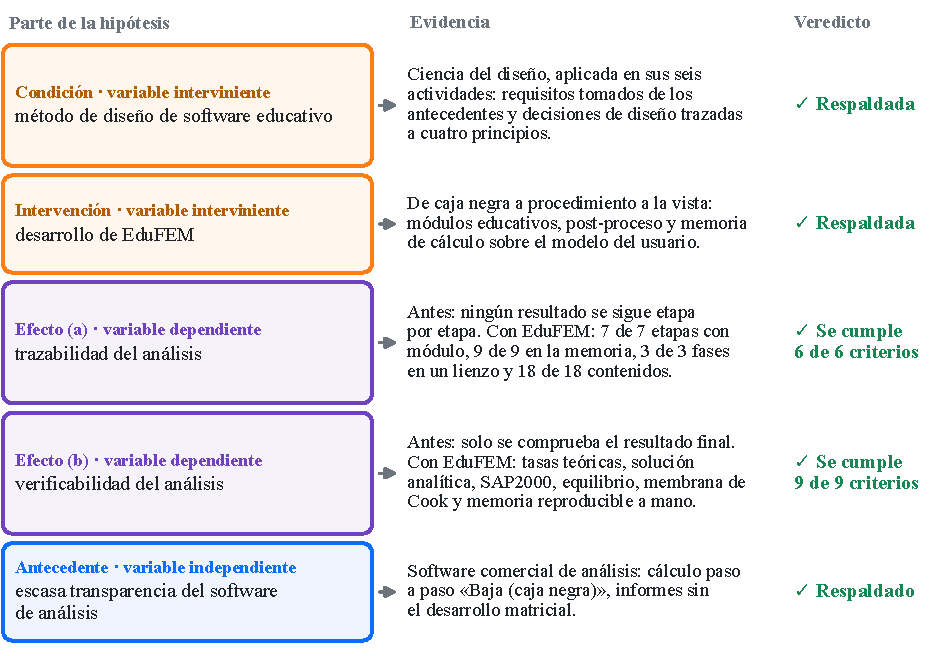
\includegraphics[width=\linewidth]{fig_contraste_hipotesis.pdf}
\caption[La hipótesis, parte por parte.]{La hipótesis, parte por parte: el papel de cada una, su evidencia y su veredicto. El enunciado está en la Introducción (\emph{Hipótesis}) y en la \autoref{sec:validacion-hipotesis}; las cifras proceden de la \autoref{tab:veredicto}, la situación de partida de la \autoref{tab:comparativa} y los veredictos de la \autoref{tab:componentes-hipotesis}.}
\label{fig:contraste-hipotesis}
\end{figure}

De la fundamentación teórica (\autoref{cap:marco_teorico}) se concluye que el software comercial de análisis opera como una caja negra y que ningún recurso educativo revisado documenta a la vez los atributos que harían trazable y verificable el procedimiento de cálculo (\autoref{tab:comparativa}). De esa brecha salieron los requisitos de la herramienta (\autoref{sec:requisitos}).

Del desarrollo de EduFEM (\autoref{cap:diseno}) se concluye que el software lleva su procedimiento de cálculo a la vista: los módulos educativos exponen sobre el modelo del usuario las etapas hasta el ensamblaje, el post-proceso muestra la respuesta con sus medios de comprobación y la memoria de cálculo reconstruye todo el procedimiento con sustitución numérica (\autoref{tab:fases}; \autoref{fig:fases-lienzo}). Las decisiones de diseño que lo logran, trazadas a sus principios (\autoref{tab:principios}), son un aporte reutilizable del trabajo.

De la verificación y la validación (\autoref{cap:resultados}) se concluye que ese procedimiento es trazable y verificable (\autoref{tab:veredicto}), que los criterios numéricos se cumplen con amplio margen (\autoref{fig:margen-criterios}) y que quedan respondidas las dos preguntas de investigación. La batería que establece la verificabilidad, reproducible y publicada con el software, es otro aporte del trabajo.

\begin{figure}[!htbp]
\centering
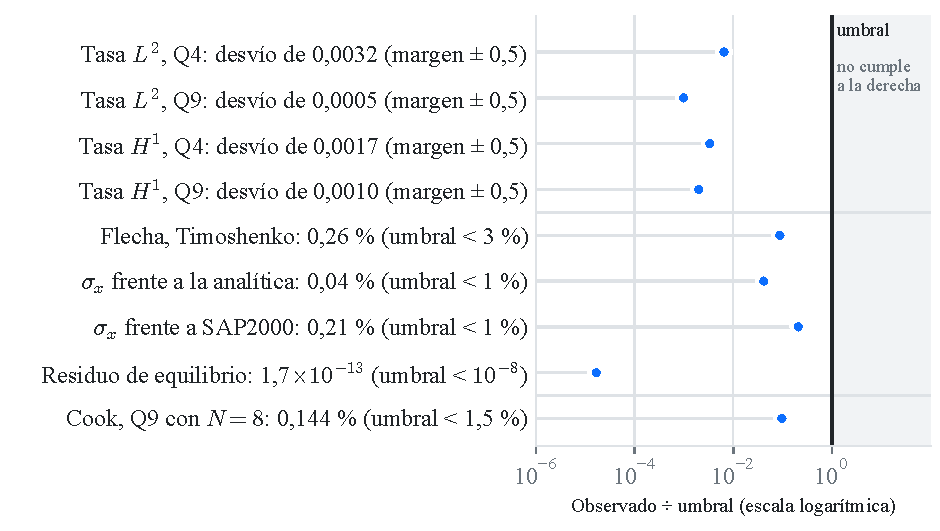
\includegraphics[width=\linewidth]{fig_margen_criterios.pdf}
\caption[Margen de cada criterio numérico de la cláusula (b).]{Margen de cada criterio numérico de la cláusula (b): el valor observado dividido por su umbral, en escala logarítmica. Todos los puntos quedan a la izquierda del umbral; cuanto más a la izquierda, más lejos del incumplimiento. En las tasas de convergencia se grafica el desvío respecto de la tasa teórica, en la peor de las cuatro configuraciones ensayadas. Las cifras son las de la \autoref{tab:veredicto}, salvo los desvíos, calculados con las tasas sin redondear.}
\label{fig:margen-criterios}
\end{figure}

El desarrollo tuvo un inconveniente: la lectura de la memoria de cálculo delató un defecto en la extrapolación de tensiones del Q4 que las pruebas de convergencia no mostraban. Se corrigió, y una prueba de la batería lo detectaría hoy (\autoref{sec:leccion-extrapolacion}); el episodio muestra, además, que exponer el procedimiento no asegura que lo expuesto sea correcto. Quedan tres debilidades, que detalla la \autoref{sec:limitaciones-observadas}: la evaluación es del autor, la deformación plana no tiene contraste externo y la exposición del procedimiento es una posibilidad que el software ofrece, no un recorrido que imponga.

% La Figura CR.2 respalda la conclusion del Cap. 3: la barrera impide que caiga
% bajo el titulo «Recomendaciones» y parta en dos la primera de ellas.
\FloatBarrier
\section*{Recomendaciones}
\phantomsection\addcontentsline{toc}{section}{Recomendaciones}

Las recomendaciones nacen de las debilidades señaladas y de las fronteras del alcance (\emph{Alcance y limitaciones}). Se agrupan por capítulo, y la \autoref{tab:triada} reúne la tríada completa.

% \needspace: el titulo de cada grupo no queda solo al pie de una hoja, separado de su
% primera recomendacion (le paso al del Cap. 3 al recortar las Conclusiones).
\needspace{4\baselineskip}
\noindent\textbf{Para la fundamentación teórica (\autoref{cap:marco_teorico}).}
\begin{itemize}
    \item \textbf{Tratamiento del bloqueo.} Incorporar la integración reducida selectiva o la formulación $\bar{\bm{B}}$ \autocites[pp.~221, 232-234]{hughes2000fem}[pp.~476-477]{bathe2014fem}, con un módulo que contraste, sobre un mismo modelo, la respuesta bloqueada y la corregida (\autoref{sec:locking}).
    \item \textbf{Más tipos de elemento.} Agregar triángulos lineales y cuadráticos, y cuadriláteros de ocho nodos y de transición \autocites[pp.~167-174, 194]{onate2009structural}{reddy2006introduction}.
\end{itemize}

\needspace{4\baselineskip}
\noindent\textbf{Para el desarrollo del software (\autoref{cap:diseno}).}
\begin{itemize}
    \item \textbf{Mallado automático.} Un generador sobre el contorno dibujado en el lienzo, controlado por las métricas de calidad del módulo M0.
    \item \textbf{Solucionador para mallas muy grandes.} Una factorización de Cholesky y un solucionador iterativo precondicionado (\autoref{tab:tiempos}), sin perder la versión legible del ensamblaje.
    \item \textbf{Guía docente.} Una secuencia de prácticas que acompañe al manual del \autoref{anexo:manual}, como rehacer a mano una etapa de la memoria del ejemplo guía.
    \item \textbf{Extensión a tres dimensiones.} Hexaedros y tetraedros, que se formulan con la misma base isoparamétrica.
\end{itemize}

\needspace{4\baselineskip}
\noindent\textbf{Para la verificación y la validación (\autoref{cap:resultados}).}
\begin{itemize}
    \item \textbf{Ampliación de la batería.} Agregar un caso civil en deformación plana con solución publicada, un caso con carga superficial linealmente variable y una prueba propia del término de cortante de la matriz de deformación plana, y medir el error de tensiones del Q4 sin la franja de contorno (\autoref{sec:mms}).
    \item \textbf{Revisión independiente.} Someter la tabla de cobertura al juicio de docentes o de especialistas en el MEF, y el código del motor a una revisión por terceros. El uso de la herramienta en el aula queda para una investigación educativa distinta.
\end{itemize}

\begin{table}[H]
\centering
\caption[La tríada: capítulo, conclusión y recomendaciones.]{La tríada del trabajo. Cada fila se lee de izquierda a derecha: el capítulo y el objetivo específico que cumple, la conclusión que establece con la evidencia que la respalda, y las recomendaciones que deja.}
\label{tab:triada}
{\footnotesize
\setlength{\tabcolsep}{3pt}
\renewcommand{\arraystretch}{1.25}
\begin{tabular}{@{}>{\raggedright\arraybackslash}p{2.7cm}@{\hspace{4pt}$\rightarrow$\hspace{4pt}}>{\raggedright\arraybackslash}p{6.3cm}@{\hspace{4pt}$\rightarrow$\hspace{4pt}}>{\raggedright\arraybackslash}p{5.2cm}@{}}
\toprule
\textbf{Capítulo y objetivo} & \textbf{Conclusión y evidencia} & \textbf{Recomendaciones} \\
\midrule
\autoref{cap:marco_teorico}. Fundamentar (cumplido) & Ningún recurso revisado documenta a la vez los atributos que harían trazable y verificable el procedimiento; de esa brecha salen los requisitos (\autoref{tab:comparativa}; \autoref{sec:requisitos}) & Tratar el bloqueo (integración reducida selectiva, $\bar{\bm{B}}$) y ampliar la biblioteca de elementos \\
\autoref{cap:diseno}. Desarrollar (cumplido) & EduFEM expone el procedimiento a la vista sobre el modelo del usuario: módulos y post-proceso sobre un mismo lienzo, y memoria de cálculo (\autoref{tab:fases}; \autoref{fig:fases-lienzo}) & Mallado automático, solucionador para mallas muy grandes, guía docente y extensión a tres dimensiones \\
\autoref{cap:resultados}. Verificar y validar (cumplido) & El procedimiento es trazable y verificable: se cumplen todos los criterios de aceptación (\autoref{tab:veredicto}; \autoref{fig:contraste-hipotesis}; \autoref{fig:margen-criterios}) & Ampliar la batería (deformación plana, carga variable) y someter la tabla de cobertura y el código a revisión independiente \\
\bottomrule
\end{tabular}}
\end{table}

\endgroup


% ----- Referencias bibliograficas (Vancouver; la norma se declara en la Introduccion, 'Normas de citacion y presentacion') -----
\cleardoublepage
\printbibliography[title={Referencias bibliográficas},heading=bibintoc]

% ----- Anexos -----
\appendix
\renewcommand{\appendixname}{Anexo}  % rotular "Anexo A/B/..." (no el "Apéndice" por defecto de babel)
% =====================================================================
%  capitulos/06_anexos.tex  --  Anexos (A, B, C, ...)
%  Va después de \appendix en main.tex (que los numera A, B, ...); el rótulo
%  "Anexo" lo fija \renewcommand{\appendixname}{Anexo} en main.tex.
% =====================================================================

\chapter{Manual de instalación}
\label{anexo:instalacion}

EduFEM se distribuye por dos vías: un instalador para Windows —la vía recomendada para el estudiante—, que despliega el software como paquete autocontenido, y la instalación desde el código fuente para su inspección o extensión. El código está disponible en el repositorio público del proyecto\footnote{Repositorio del proyecto: \url{https://github.com/Sucullani/SoftwareED}}.

\section{Instalación en Windows}

EduFEM se distribuye como un instalador único (\texttt{EduFEM-Setup.exe}) que copia el software, crea accesos directos en el menú Inicio y en el escritorio —identificados por el icono de la herramienta (\autoref{fig:logo-edufem})—, asocia la extensión \texttt{.edufem} de los proyectos para que se abran con doble clic y registra un desinstalador. La instalación se realiza por usuario, sin privilegios de administrador. Requisito: Windows 10 u 11 de 64 bits.

El paquete es autosuficiente en un sentido estricto: el empaquetado con \texttt{PyInstaller} incorpora el intérprete de Python y todas las bibliotecas, y el instalador añade la distribución \LaTeX{} reducida que describe la \autoref{sec:stack}, instalada junto al ejecutable. En consecuencia, el equipo de destino no necesita Python, ni una distribución \LaTeX{} previa, ni conexión a internet durante la instalación o el uso. Esta decisión responde a una dificultad observada en la práctica: cuando la memoria de cálculo se compilaba con la distribución \LaTeX{} que hubiera en el equipo, una instalación mínima interrumpía la exportación con un cuadro de diálogo por cada paquete ausente. Si falta la carpeta con el motor \LaTeX{}, el software recurre a la distribución que encuentre instalada en el sistema y, en su defecto, informa el problema; las fórmulas que se muestran en pantalla no dependen de \LaTeX{} en ningún caso.

Una restricción heredada de \TeX{} Live condiciona la carpeta de instalación: su motor no resuelve rutas que contengan tildes o espacios. Como el destino habitual de una instalación por usuario incluye el nombre del perfil de Windows, el asistente comprueba si esa ruta contiene tildes o espacios y, en ese caso, propone instalar en \texttt{C:\textbackslash ProgramData\textbackslash EduFEM}, que un usuario sin privilegios puede crear igualmente.

Al no estar firmado con un certificado comercial, la primera ejecución del instalador puede mostrar el aviso de Microsoft Defender SmartScreen (\enquote{Windows protegió su PC}), habitual en aplicaciones nuevas; se continúa con \emph{Más información} y \emph{Ejecutar de todas formas}. Una vez instalado, EduFEM se abre desde su icono como cualquier otra aplicación, sin nuevos avisos.

\section{Instalación desde el código fuente}

Para docentes o desarrolladores que deseen inspeccionar o modificar el software:

\begin{enumerate}
    \item Instalar \textbf{Python 3.11 o superior} (el desarrollo se realizó con la versión 3.13).
    \item Clonar el repositorio y ubicarse en su carpeta:
\begin{verbatim}
git clone https://github.com/Sucullani/SoftwareED.git
cd SoftwareED
\end{verbatim}
    \item Crear y activar un entorno virtual (recomendado):
\begin{verbatim}
python -m venv .venv
.venv\Scripts\activate
\end{verbatim}
    \item Instalar las dependencias:
\begin{verbatim}
pip install -r requirements.txt
\end{verbatim}
    \item Ejecutar EduFEM:
\begin{verbatim}
python main.py
\end{verbatim}
\end{enumerate}

\section{Dependencias}

El núcleo numérico y la interfaz se apoyan en bibliotecas de código abierto: NumPy y SciPy (cálculo), \texttt{ttkbootstrap} (interfaz), \texttt{pylatex} (memoria de cálculo y documentos de teoría), \texttt{Pillow} (figuras) y \texttt{ezdxf} (importación DXF). A ellas se añaden \texttt{matplotlib}, para los gráficos de los módulos educativos, la vista 3D y el círculo de Mohr, y \texttt{sympy}, para las expresiones simbólicas de los módulos y de la memoria de cálculo. A ellas se suma un componente externo al ecosistema de Python: el motor \texttt{pdflatex} que compila la memoria de cálculo, provisto por la distribución \LaTeX{} reducida que acompaña al instalador. Quien trabaje desde el código fuente puede generar esa distribución con el guion incluido en el repositorio o bien apoyarse en una instalación de \LaTeX{} propia. El motor numérico está vectorizado por lotes en NumPy puro ---calcula todos los elementos a la vez con operaciones sobre arreglos, en lugar de recorrerlos uno por uno---; así, las mediciones de tiempo del \autoref{cap:resultados} se reproducen con las dependencias listadas, sin compiladores ni aceleradores adicionales.


\chapter{Manual de uso}
\label{anexo:manual}

Este anexo describe el trabajo con EduFEM, desde la construcción del modelo hasta la interpretación de los resultados. El diseño de cada componente y su justificación están en la \autoref{sec:diseno-edufem}; aquí se indica cómo operarlo. El software organiza ese trabajo en tres fases ---pre-proceso, proceso y post-proceso--- accesibles mediante pestañas, que comparten un único lienzo central, es decir, el área gráfica donde se dibuja el modelo. La barra de menús se reduce deliberadamente a tres entradas: \textsf{Archivo}, \textsf{Modelo} y \textsf{Ayuda}.

La \autoref{fig:app-completa} muestra la ventana principal en la fase de pre-proceso, con sus tres zonas: el cuaderno de tablas, el lienzo compartido y la barra de estado.

\begin{figure}[htbp]
\centering
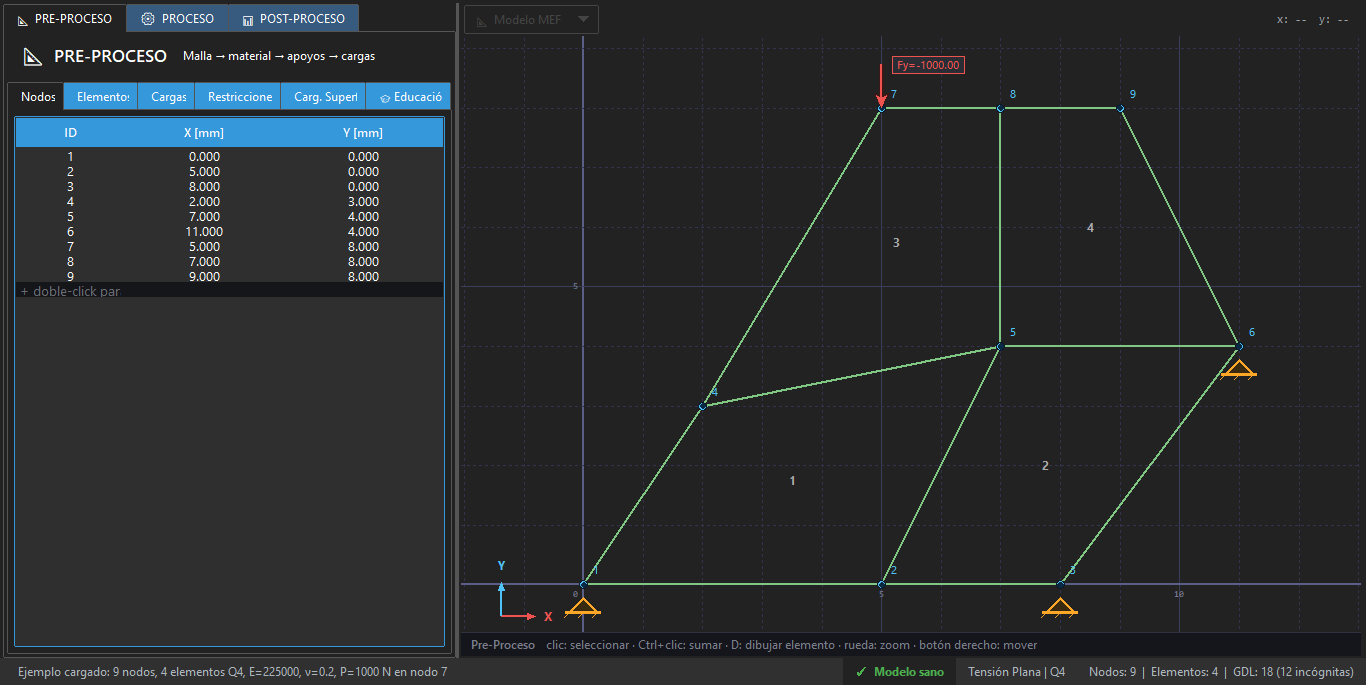
\includegraphics[width=\linewidth]{fig_app_completa}
\caption[Ventana principal de EduFEM en la fase de pre-proceso.]{Ventana principal de EduFEM en la fase de pre-proceso. A la izquierda, el cuaderno de tablas editables (con la tabla de \textsf{Nodos} activa); a la derecha, el lienzo compartido con el modelo del ejemplo guía ---nodos, elementos, la carga nodal, los apoyos y los ejes---. La barra de estado inferior resume el diagnóstico de salud, el tipo de análisis y el recuento de grados de libertad.}
\label{fig:app-completa}
\end{figure}

\section{Pre-proceso: construcción del modelo}

La fase de pre-proceso (identidad cromática azul) reúne la definición geométrica y de cargas. A la izquierda, un cuaderno de cinco tablas editables ---\textsf{Nodos}, \textsf{Elementos}, \textsf{Cargas}, \textsf{Restricciones} y \textsf{Carg.\ Superf.}--- permite la entrada y edición directa de cada entidad; a la derecha, el lienzo refleja el modelo en tiempo real.

\subsection{Definición de la geometría}

Existen tres vías para construir la malla:

\begin{itemize}
  \item \textbf{Edición en tablas.} El doble clic en una celda abre el editor, y el doble clic en la fila atenuada del pie de cada tabla (\emph{placeholder}, es decir, la fila que reserva el lugar del registro siguiente) crea un registro nuevo con valores por defecto, que luego se completa. Se admite el pegado de bloques de texto tabulado desde una hoja de cálculo (Ctrl+V) para el alta masiva.
  \item \textbf{Modo dibujo (tecla D).} Al estilo de un programa de dibujo asistido, el usuario marca cuatro vértices sobre el lienzo ---con anclaje automático a los nodos existentes--- y el elemento cuadrilátero se crea al cuarto clic, corrigiendo de oficio la orientación antihoraria.
  \item \textbf{Importación.} Desde \textsf{Archivo} $\rightarrow$ \textsf{Importar} se carga geometría en formato DXF (polilíneas cerradas de cuatro vértices en la capa \texttt{FEM\_ELEMENTS}) o las entidades de un modelo en CSV/Excel.
\end{itemize}

\subsection{Propiedades del modelo}

El menú \textsf{Modelo} agrupa, en el orden lógico de definición de un problema de elementos finitos, cinco diálogos: \textsf{Tipo de Elemento} (Q4 o Q9), \textsf{Unidades} (ocho sistemas predefinidos con conversión automática de los valores), \textsf{Materiales} (módulo de elasticidad $E$, coeficiente de Poisson $\nu$ y densidad $\rho$), \textsf{Gravedad} (vector de aceleración y su activación) y \textsf{Tipo de Análisis} (tensión o deformación plana). Al cambiar de Q4 a Q9, los cinco nodos adicionales por elemento ---cuatro de arista y el central--- se generan automáticamente. La \autoref{fig:dialogo-material} muestra, a modo de ejemplo, el diálogo de materiales.

\begin{figure}[htbp]
\centering
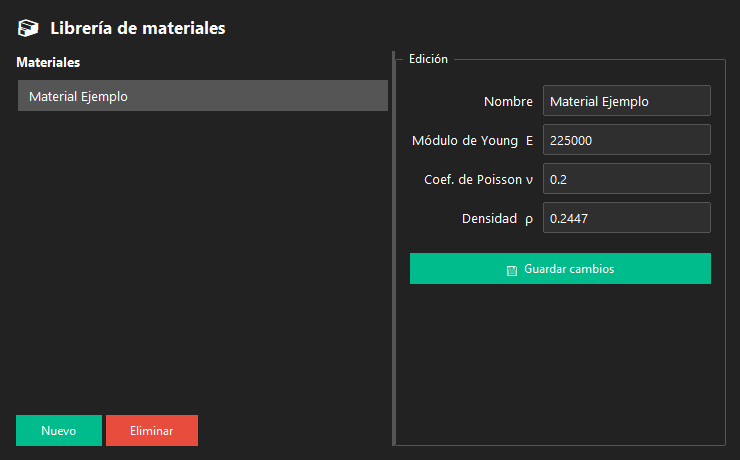
\includegraphics[width=0.72\linewidth]{fig_dialogo_material}
\caption[Diálogo de materiales.]{Diálogo \textsf{Modelo} $\rightarrow$ \textsf{Materiales}: la lista de materiales definidos a la izquierda y el formulario de propiedades ($E$, $\nu$, $\rho$) a la derecha.}
\label{fig:dialogo-material}
\end{figure}

El diálogo \textsf{Tipo de Análisis} (\autoref{fig:dialogo-analisis}) ilustra con animaciones la distinción entre tensión plana ($\sigma_z = 0$) y deformación plana ($\varepsilon_z = 0$), las dos hipótesis bidimensionales que el software resuelve.

\begin{figure}[htbp]
\centering
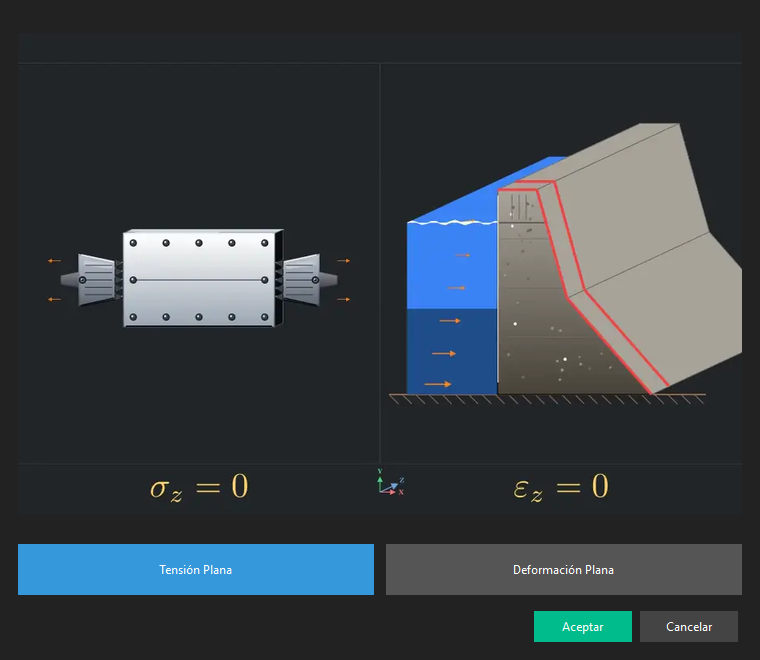
\includegraphics[width=0.72\linewidth]{fig_dialogo_analisis}
\caption[Diálogo del tipo de análisis.]{Diálogo \textsf{Modelo} $\rightarrow$ \textsf{Tipo de Análisis}: la selección entre tensión plana (placa delgada cargada en su plano, $\sigma_z = 0$) y deformación plana (sólido largo confinado, $\varepsilon_z = 0$), con una animación ilustrativa de cada hipótesis.}
\label{fig:dialogo-analisis}
\end{figure}

\subsection{Cargas y restricciones}

Las cargas nodales, las cargas de superficie (carga distribuida sobre una arista, con su ángulo de aplicación) y las restricciones (empotramiento, rodillo en $x$ o en $y$) se definen en sus tablas respectivas o seleccionando la entidad en el lienzo, que pre-rellena una fila «fantasma» con valores por defecto. Los símbolos siguen la convención estructural habitual: triángulo con achurado para el empotramiento y triángulo sobre rodillo para los apoyos deslizantes.

\section{Proceso: resolución y exploración didáctica}

La fase de proceso (identidad cromática naranja) alberga los módulos educativos. La tecla F5, o el cambio a la pestaña de post-proceso, dispara la resolución, que antes revisa el modelo con un comprobador de salud (\autoref{fig:validador-salud}). Un error crítico detiene la resolución y se reporta con sugerencias de corrección; el usuario solo puede continuar si elige \textsf{Resolver de todos modos}, y ni así cuando faltan los elementos o las restricciones. Las advertencias no detienen la resolución.

\begin{figure}[!htb]
\centering
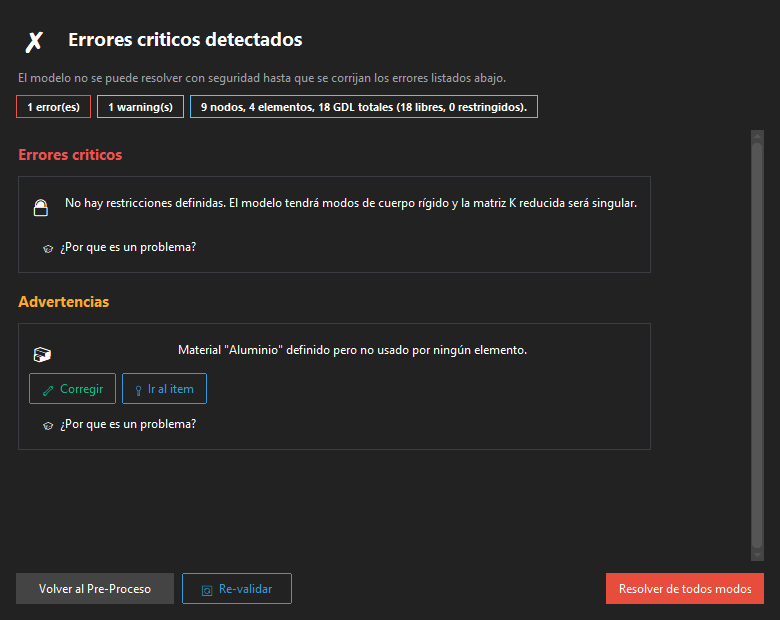
\includegraphics[width=0.82\linewidth]{fig_validador_salud}
\caption[Comprobador de salud del modelo.]{Comprobador de salud del modelo. Los errores críticos ---aquí, la ausencia de restricciones, que volvería singular la matriz de rigidez reducida--- detienen la resolución y se acompañan de una explicación; con \textsf{Resolver de todos modos} el usuario puede continuar, salvo, como en este caso, cuando faltan las restricciones o los elementos. Las advertencias no detienen la resolución. Cada hallazgo ofrece, cuando procede, corrección automática y navegación a la entidad implicada.}
\label{fig:validador-salud}
\end{figure}

Siete módulos educativos (M1 a M7), accesibles con Ctrl+1 a Ctrl+7, recorren en orden el procedimiento de cálculo, es decir, la secuencia de etapas que va de las funciones de forma a la recuperación de tensiones; un octavo (M0) atiende la calidad de malla en el pre-proceso. La \autoref{sec:catalogo-modulos-edu} describe el catálogo completo y reproduce cada módulo en funcionamiento.

\section{Post-proceso: interpretación de resultados}

La fase de post-proceso (identidad cromática verde) superpone los resultados sobre el mismo lienzo. El panel de control permite alternar entre los campos de tensión ---$\sigma_x$, $\sigma_y$, $\tau_{xy}$, las principales $\sigma_1$ y $\sigma_2$ y la de von Mises--- y de desplazamiento, mostrar la malla deformada con un factor de amplificación regulable, activar isolíneas y abrir una vista tridimensional del campo. El sondeo puntual informa, en cualquier punto del dominio, el estado tensional completo y, con el clic derecho, despliega un panel de detalles con el círculo de Mohr del punto consultado. Los valores de la tabla de resultados se copian al portapapeles con Ctrl+C en un formato compatible con hoja de cálculo. La \autoref{fig:vista3d} muestra la vista tridimensional del campo, una representación alternativa del mismo resultado que el contorno 2D.

\begin{figure}[htbp]
\centering
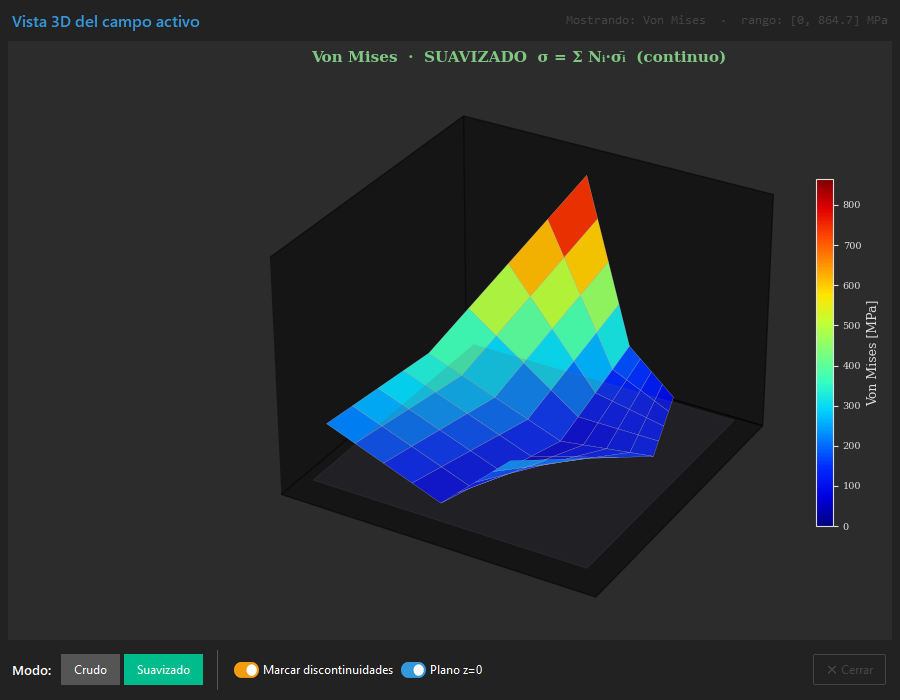
\includegraphics[width=0.82\linewidth]{fig_vista3d}
\caption[Vista 3D del campo de von Mises.]{Vista 3D del campo de tensión de von Mises sobre el ejemplo guía, en modo \textsf{Suavizado}. El conmutador \textsf{Crudo}\,/\,\textsf{Suavizado} alterna entre el campo evaluado dentro de cada elemento, discontinuo entre elementos, y el campo nodal promediado; las casillas permiten marcar discontinuidades y el plano de referencia $z=0$.}
\label{fig:vista3d}
\end{figure}

\section{Documentación del cálculo e intercambio de datos}

Desde \textsf{Archivo} $\rightarrow$ \textsf{Exportar} se genera la memoria de cálculo en PDF, un documento que reproduce el paso a paso simbólico y numérico del modelo concreto del usuario ---funciones de forma evaluadas en los puntos de Gauss, Jacobiano, matrices $\bm{B}$ y $\bm{D}$, rigidez elemental, ensamblaje, partición de restricciones, resolución y recuperación de tensiones--- en dos estilos, educativo o directo. El mismo menú exporta el modelo a CSV/Excel para su edición masiva. Los proyectos se guardan en el formato nativo \texttt{.edufem}.

\section{Atajos de teclado}

La \autoref{tab:atajos} reúne los atajos de teclado del software.

\begin{table}[htbp]
\centering
\caption[Atajos de teclado de EduFEM.]{Atajos de teclado de EduFEM: la primera columna da la combinación y la segunda, la acción que dispara. Los atajos \texttt{Ctrl+1} a \texttt{Ctrl+7} abren los módulos educativos M1 a M7 en la fase de proceso.}
\label{tab:atajos}
\begin{tabular}{l l}
\hline
Atajo & Acción \\
\hline
Ctrl+N / O / S / Shift+S & Nuevo / Abrir / Guardar / Guardar Como \\
Ctrl+E                   & Cargar ejemplo \\
Ctrl+Z                   & Deshacer \\
Ctrl+Y o Ctrl+Shift+Z    & Rehacer \\
Ctrl+C / V               & Copiar / Pegar (texto tabulado) \\
Ctrl+1 \dots\ 7          & Módulos educativos M1 a M7 \\
F5                       & Resolver \\
F11 / F                  & Pantalla completa / Ajustar vista \\
D                        & Modo dibujo de elementos \\
Ctrl+clic / Shift+clic   & Selección múltiple (alternar / rango) \\
Esc                      & Cancelar elemento, cerrar editor o limpiar selección \\
Ctrl+Tab / Ctrl+Shift+Tab & Pestaña siguiente / anterior \\
Ctrl+/, F1               & Atajos / Manual \\
Ctrl+A                   & Seleccionar toda la tabla de resultados \\
F8                       & Modo ortogonal al dibujar (Shift lo invierte) \\
Retroceso                & Borrar el último vértice del elemento parcial \\
Supr                     & Eliminar la entidad seleccionada \\
Ctrl+Q                   & Salir \\
\hline
\end{tabular}
\end{table}

\section{Casos de ejemplo}

El submenú \textsf{Ayuda} $\rightarrow$ \textsf{Cargar Ejemplo} (atajo Ctrl+E para el ejemplo guía) ofrece tres modelos de ejemplo precargados, cada uno en variante Q4 y Q9. El primero es el \textbf{ejemplo guía} (cuatro elementos y nueve nodos en su variante Q4; es el primer caso de prueba del proyecto y el de la memoria del \autoref{anexo:memoria}), que el menú rotula \textsf{Cuadrado de validación}. Los otros dos son la \textbf{viga de Timoshenko} (simplemente apoyada, contrastada con la solución analítica y con SAP2000) y la \textbf{membrana de Cook} (trapecio que ilustra el bloqueo por cortante). Estos casos sirven de punto de partida para explorar todas las funciones descritas.


\section{Catálogo de módulos educativos}
\label{sec:catalogo-modulos-edu}

EduFEM organiza su contenido didáctico en ocho módulos educativos, distribuidos según las fases del procedimiento de cálculo del MEF. Cada módulo es una capa interactiva que se superpone sobre el lienzo donde se dibuja la malla: en lugar de presentar la teoría en una ventana aislada, ilumina, anota o anima directamente el elemento o la malla que el usuario tiene en pantalla. Los de las matrices $\bm{J}$, $\bm{B}$ y $\bm{D}$ (M2 a M4) ofrecen además un conmutador Fórmula\,$\leftrightarrow$\,Valores, que alterna entre la expresión simbólica y su evaluación numérica en el punto seleccionado. El primer módulo (M0) corresponde a la fase de pre-proceso y opera sobre la malla completa, mientras que los siete restantes (M1 a M7) acompañan la fase de proceso siguiendo el orden del cálculo. La fase de post-proceso no incorpora módulos: el análisis de resultados se realiza con las herramientas nativas del post-proceso (contorno, sonda de tensiones, círculo de Mohr y vista 3D). La \autoref{tab:modulos-edu} resume el catálogo completo, indicando para cada módulo su fase, el concepto del MEF que ilustra y el atajo de teclado asociado.

\begin{table}[htbp]
\centering
\caption[Catálogo de los ocho módulos educativos de EduFEM.]{Catálogo de los ocho módulos educativos de EduFEM, ordenados según el procedimiento de cálculo del MEF. Para cada módulo se indican la fase de la interfaz en que se abre, el concepto que expone y el atajo de teclado. M0 es global del pre-proceso y carece de atajo numérico; M1 a M7 siguen el orden del cálculo, con atajos \texttt{Ctrl+1} a \texttt{Ctrl+7}.}
\label{tab:modulos-edu}
\begin{tabular}{l l p{6.2cm} l}
\toprule
\textbf{Módulo} & \textbf{Fase} & \textbf{Concepto del MEF} & \textbf{Atajo} \\
\midrule
M0 & Pre-proceso  & Calidad de malla: Jacobiano escalado y compacidad (\emph{stretch}). & --- \\
M1 & Proceso      & Mapeo isoparamétrico y funciones de forma $N$: coordenadas naturales $(\xi,\eta) \leftrightarrow (x,y)$. & \texttt{Ctrl+1} \\
M2 & Proceso      & Jacobiano $\det\bm{J}(\xi,\eta)$: distorsión local, superficie 3D. & \texttt{Ctrl+2} \\
M3 & Proceso      & Matriz $\bm{B}$ (deformación): $\partial N/\partial x$ mediante $\bm{J}^{-1}$, con anclaje a puntos de Gauss. & \texttt{Ctrl+3} \\
M4 & Proceso      & Matriz constitutiva $\bm{D}(E,\nu,\text{caso})$ según el material del elemento. & \texttt{Ctrl+4} \\
M5 & Proceso      & Rigidez $\bm{k}_e$ y cuadratura de Gauss: la integral, sin primitiva practicable en un elemento de geometría arbitraria, se aproxima como suma en los puntos de Gauss. & \texttt{Ctrl+5} \\
M6 & Proceso      & Fuerzas equivalentes nodales: carga sobre arista y peso propio. & \texttt{Ctrl+6} \\
M7 & Proceso      & Ensamblaje de $\bm{K}$ y $\bm{F}$ con restricciones: esqueleto de $\bm{K}$ y aporte de cada elemento a sus filas y columnas. & \texttt{Ctrl+7} \\
\bottomrule
\end{tabular}
\end{table}


De la \autoref{fig:mod-m0} a la \autoref{fig:mod-m7} se reproduce cada módulo en funcionamiento sobre el ejemplo guía, con capturas tomadas directamente del software: a la izquierda, el lienzo con el elemento bajo análisis y la iluminación que el módulo proyecta sobre la malla; a la derecha, el panel flotante con su contenido (fórmulas, matrices o controles interactivos). Para cada captura, el texto indica el rasgo concreto que conviene observar en ella.

\begin{figure}[htbp]
\centering
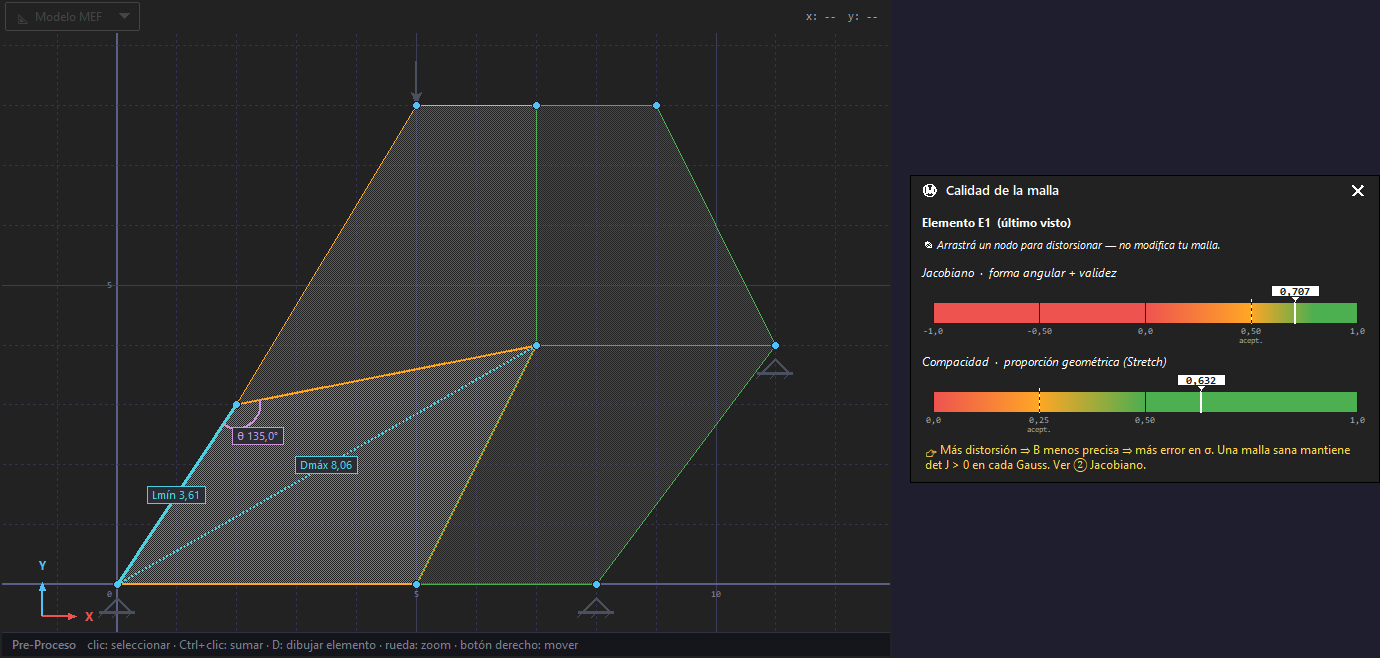
\includegraphics[width=\linewidth]{fig_modulo_m0}
\caption[Módulo M0 (calidad de malla).]{Módulo M0 (calidad de malla). Vista de rayos X de la malla coloreada por calidad, las barras de Jacobiano escalado y compacidad (\emph{stretch}) del elemento bajo el cursor, y las anotaciones geométricas sobre el lienzo: el peor ángulo, la arista mínima $L_{\min}$ y la diagonal máxima $D_{\max}$. Cada elemento toma la peor clase de sus dos métricas: verde, buena calidad; naranja, aceptable; rojo, inadmisible, según los cortes propios del módulo (\autoref{sec:pre-proceso}).}
\label{fig:mod-m0}
\end{figure}

En la \autoref{fig:mod-m0} conviene observar la correspondencia entre el color de cada elemento y las dos barras del panel: el color resume sobre la geometría lo que las barras de Jacobiano escalado y compacidad cuantifican para el elemento bajo el cursor.

\begin{figure}[htbp]
\centering
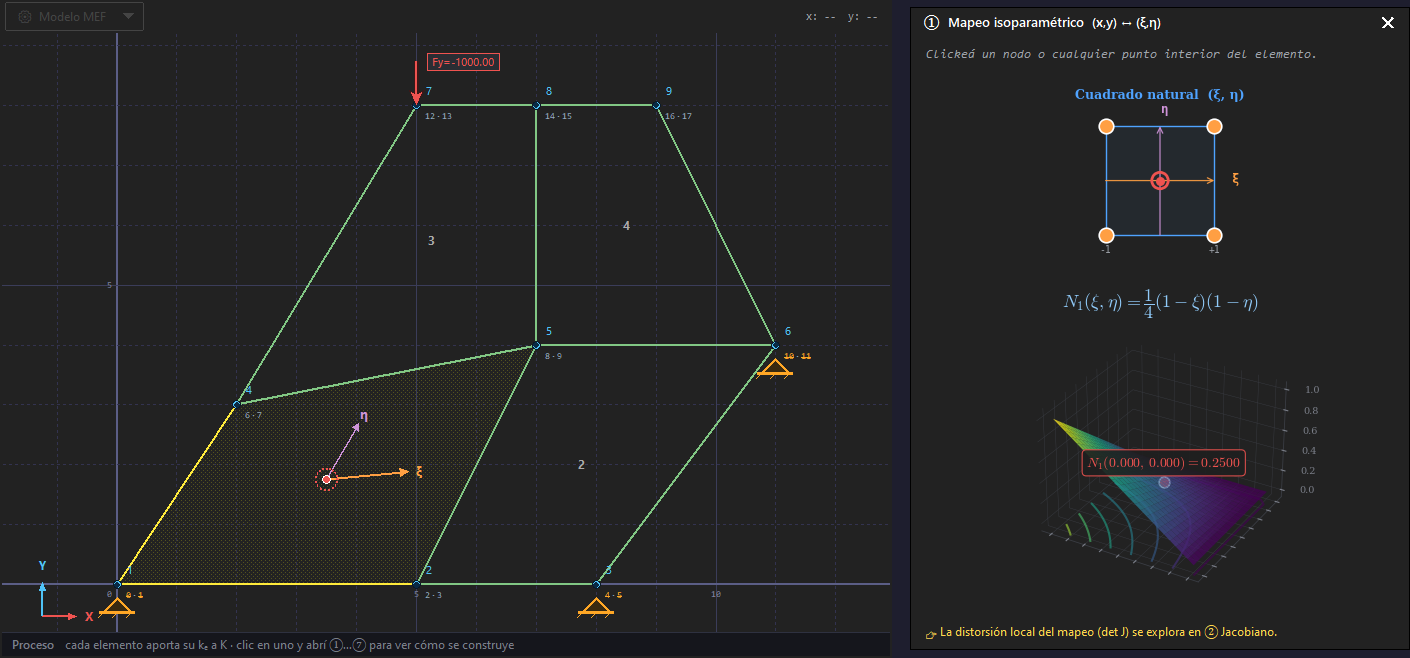
\includegraphics[width=\linewidth]{fig_modulo_m1}
\caption[Módulo M1 (mapeo isoparamétrico y funciones de forma).]{Módulo M1 (mapeo isoparamétrico y funciones de forma). El cuadrado natural $(\xi,\eta)$, la expresión de la función de forma $N_1$ y su superficie tridimensional, junto al elemento y el punto evaluado sobre el lienzo.}
\label{fig:mod-m1}
\end{figure}

El rasgo que debe seguirse en la \autoref{fig:mod-m1} es la doble marca del punto evaluado: la que aparece en el cuadrado natural $(\xi,\eta)$ y la que le corresponde sobre el elemento real del lienzo. Esa pareja de marcas es el mapeo isoparamétrico visto en un solo punto.

\begin{figure}[htbp]
\centering
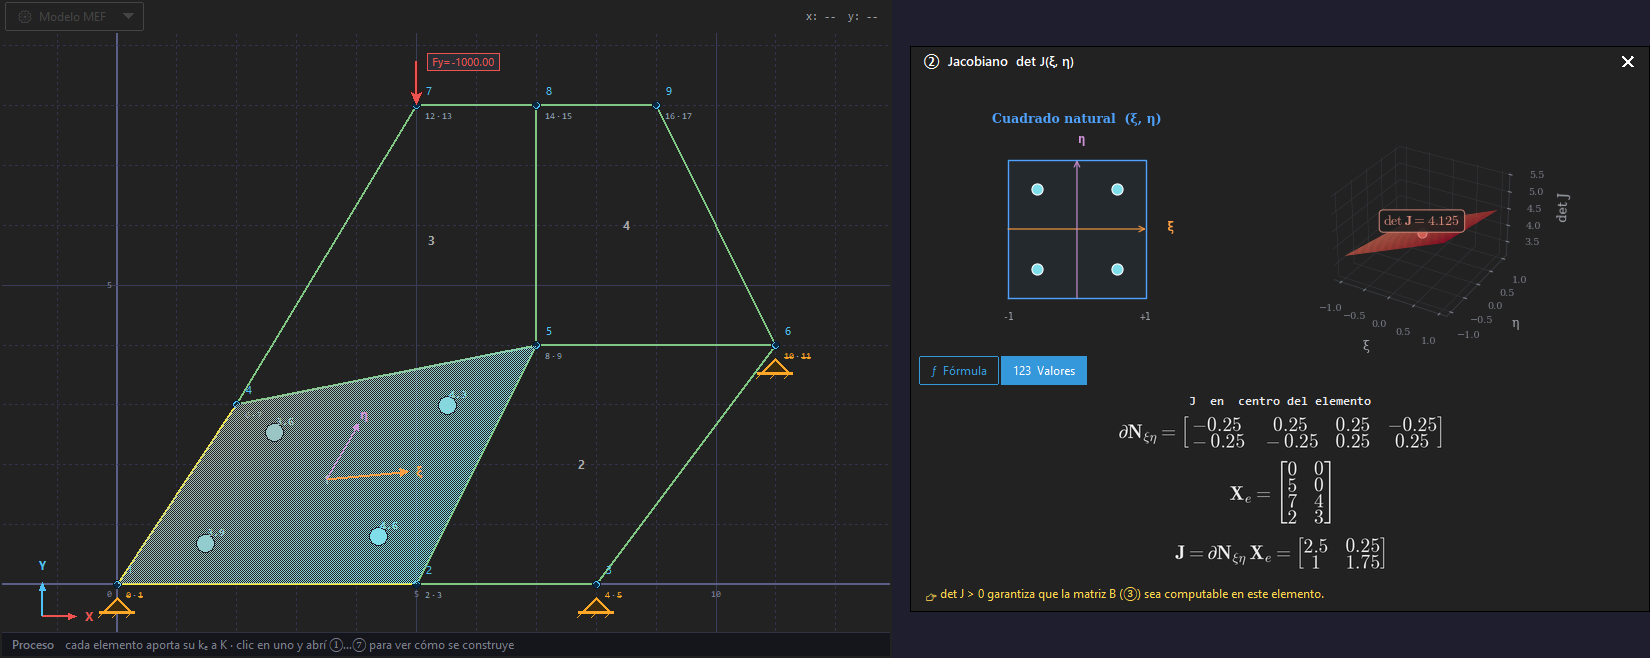
\includegraphics[width=\linewidth]{fig_modulo_m2}
\caption[Módulo M2 (Jacobiano).]{Módulo M2 (Jacobiano). El cuadrado natural con sus cuatro puntos de Gauss y la superficie 3D de $\det\bm{J}(\xi,\eta)$, evaluada aquí en el centro del elemento; sobre el lienzo, cada punto de Gauss lleva rotulado su valor de $\det\bm{J}$.}
\label{fig:mod-m2}
\end{figure}

En la \autoref{fig:mod-m2} hay que mirar la altura de la superficie de $\det\bm{J}$ sobre el cuadrado natural: es horizontal cuando el elemento es un paralelogramo y se inclina a medida que sus lados opuestos dejan de ser paralelos; las zonas donde desciende son aquellas en que el mapeo comprime más la geometría. Una superficie horizontal no descarta la distorsión angular, que mide el Jacobiano escalado de M0.

\begin{figure}[htbp]
\centering
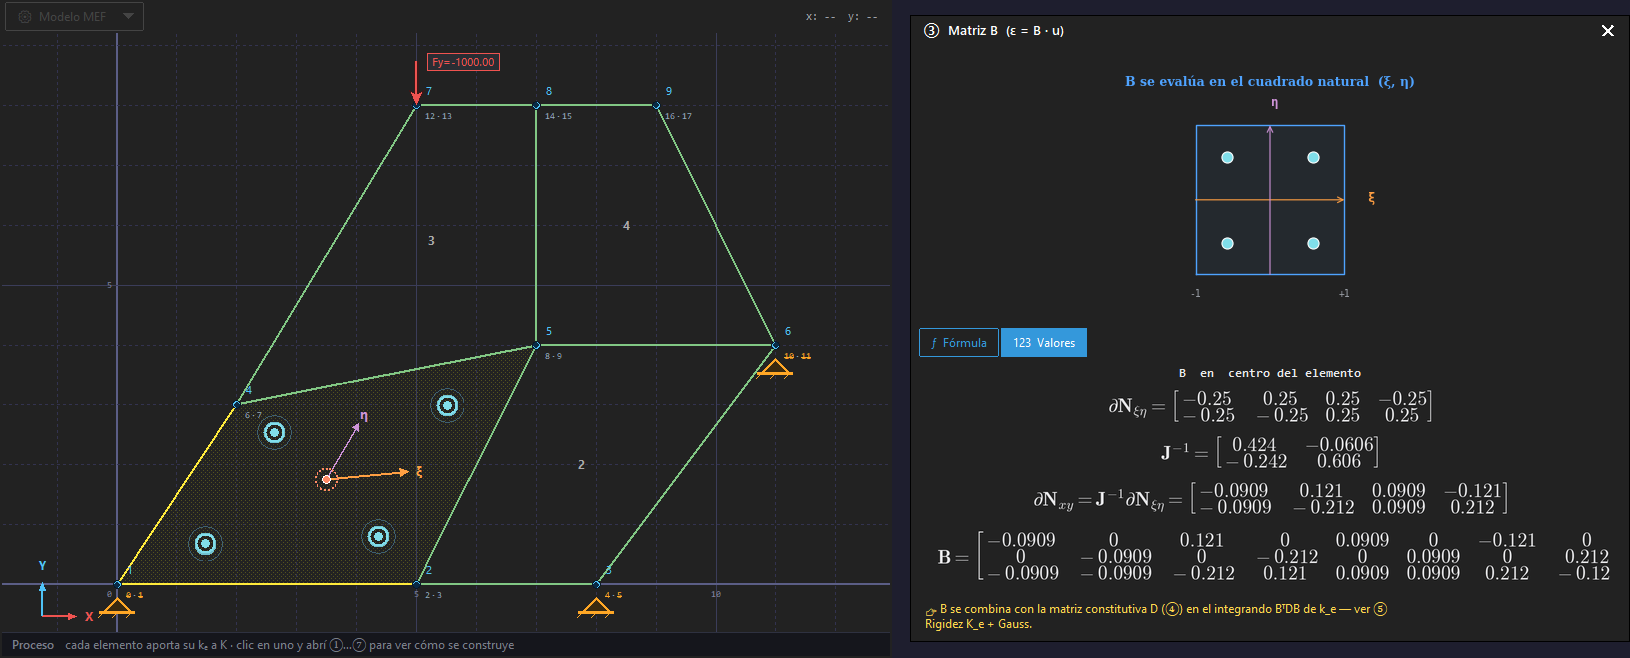
\includegraphics[width=\linewidth]{fig_modulo_m3}
\caption[Módulo M3 (matriz de deformación $\bm{B}$).]{Módulo M3 (matriz de deformación $\bm{B}$). La secuencia de derivadas $\partial\bm{N}_{\xi\eta}\to\bm{J}^{-1}\to\bm{B}$ evaluada en el punto natural, anclada a los puntos de Gauss del elemento.}
\label{fig:mod-m3}
\end{figure}

De la \autoref{fig:mod-m3} interesa la cadena de matrices del panel: las derivadas naturales, multiplicadas por $\bm{J}^{-1}$, dan las derivadas físicas, que se ordenan en $\bm{B}$. En la captura, la cadena está evaluada en el centro del elemento; un clic junto a uno de los puntos de Gauss resaltados la evalúa en ese punto.

\begin{figure}[htbp]
\centering
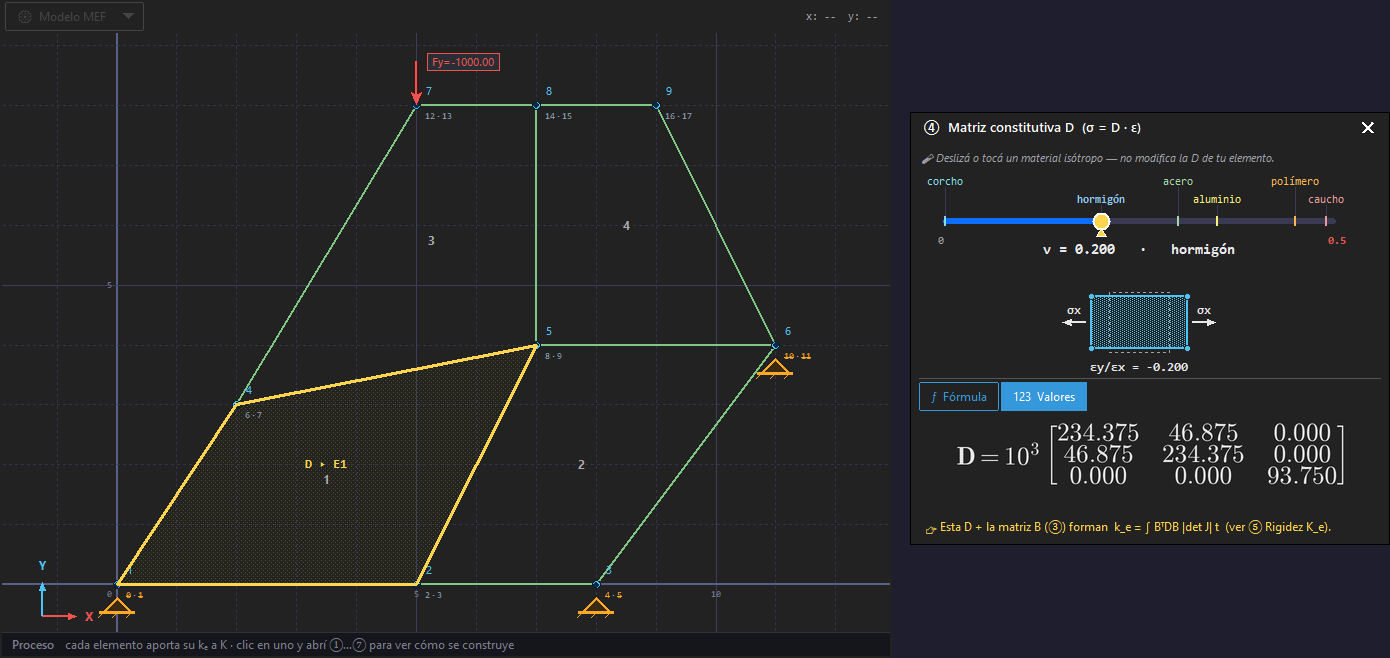
\includegraphics[width=\linewidth]{fig_modulo_m4}
\caption[Módulo M4 (matriz constitutiva $\bm{D}$).]{Módulo M4 (matriz constitutiva $\bm{D}$). El espectro del coeficiente de Poisson $\nu$ y su efecto sobre la matriz $\bm{D}$ y la deformación del elemento.}
\label{fig:mod-m4}
\end{figure}

En la \autoref{fig:mod-m4} el rasgo a observar es lo que ocurre al recorrer el espectro del coeficiente de Poisson: los coeficientes de $\bm{D}$ y la deformación dibujada sobre el elemento cambian a la vez, de modo que puede verse qué término de la matriz gobierna cada efecto.

\begin{figure}[htbp]
\centering
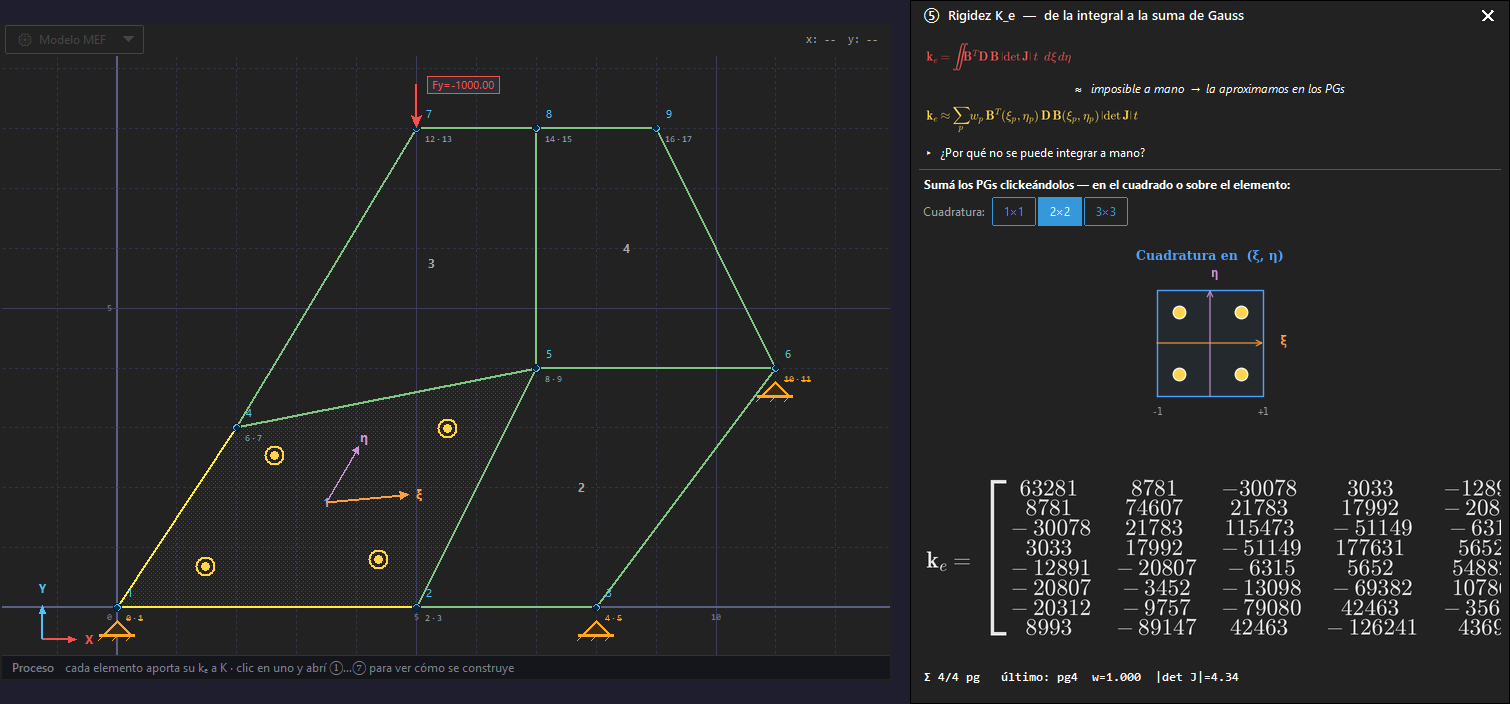
\includegraphics[width=\linewidth]{fig_modulo_m5}
\caption[Módulo M5 (rigidez $\bm{k}_e$ y cuadratura de Gauss).]{Módulo M5 (rigidez $\bm{k}_e$ y cuadratura de Gauss). El salto de la integral a la suma ($\int\!\to\!\sum$), los puntos de Gauss sobre el elemento y la matriz $\bm{k}_e$ que crece al sumar las contribuciones.}
\label{fig:mod-m5}
\end{figure}

La \autoref{fig:mod-m5} debe leerse siguiendo los puntos de Gauss del elemento: cada uno aporta un sumando a la cuadratura y, al incorporarlo, la matriz $\bm{k}_e$ del panel se actualiza. Es la traducción visual del paso de la integral a la suma.

\begin{figure}[htbp]
\centering
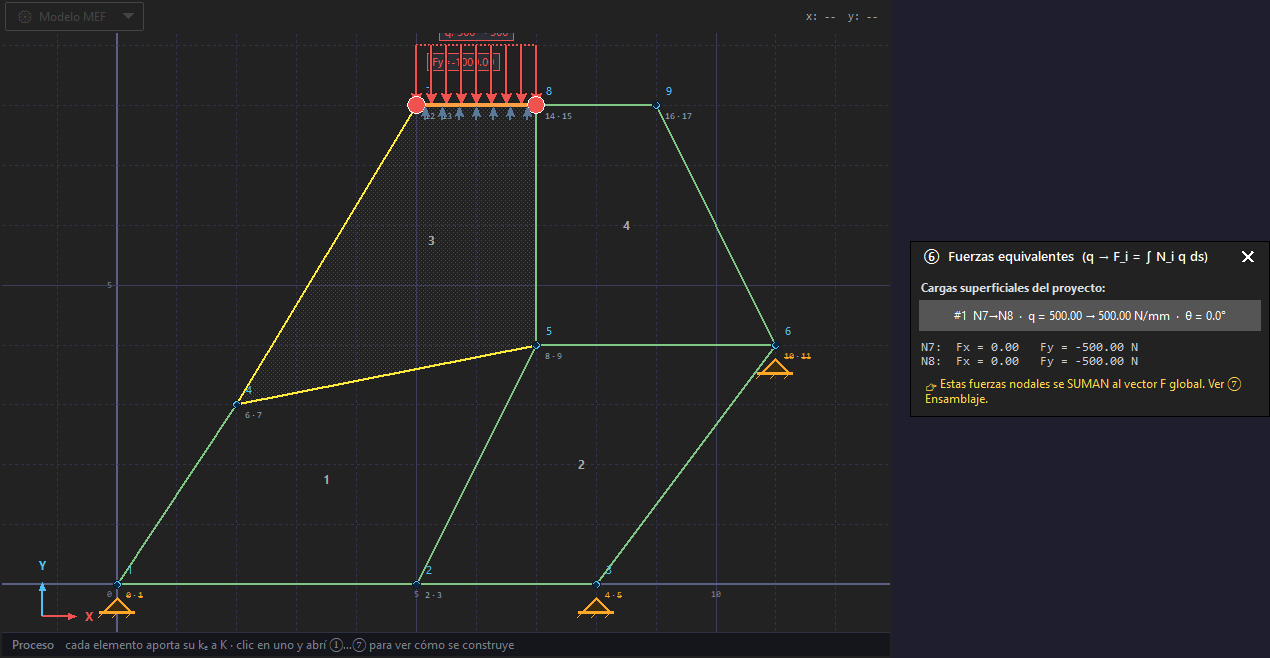
\includegraphics[width=\linewidth]{fig_modulo_m6}
\caption[Módulo M6 (fuerzas equivalentes).]{Módulo M6 (fuerzas equivalentes). Una carga superficial sobre la arista entre los nodos 7 y 8, añadida para la captura al ejemplo guía, que no la incluye, y su conversión en fuerzas nodales equivalentes mediante $F_i=\int N_i\,q\,ds$.}
\label{fig:mod-m6}
\end{figure}

En la \autoref{fig:mod-m6} conviene comparar la carga repartida sobre la arista con las fuerzas nodales que la sustituyen: el panel muestra el valor de cada una junto a la integral $F_i=\int N_i\,q\,ds$ de la que proviene.

\begin{figure}[htbp]
\centering
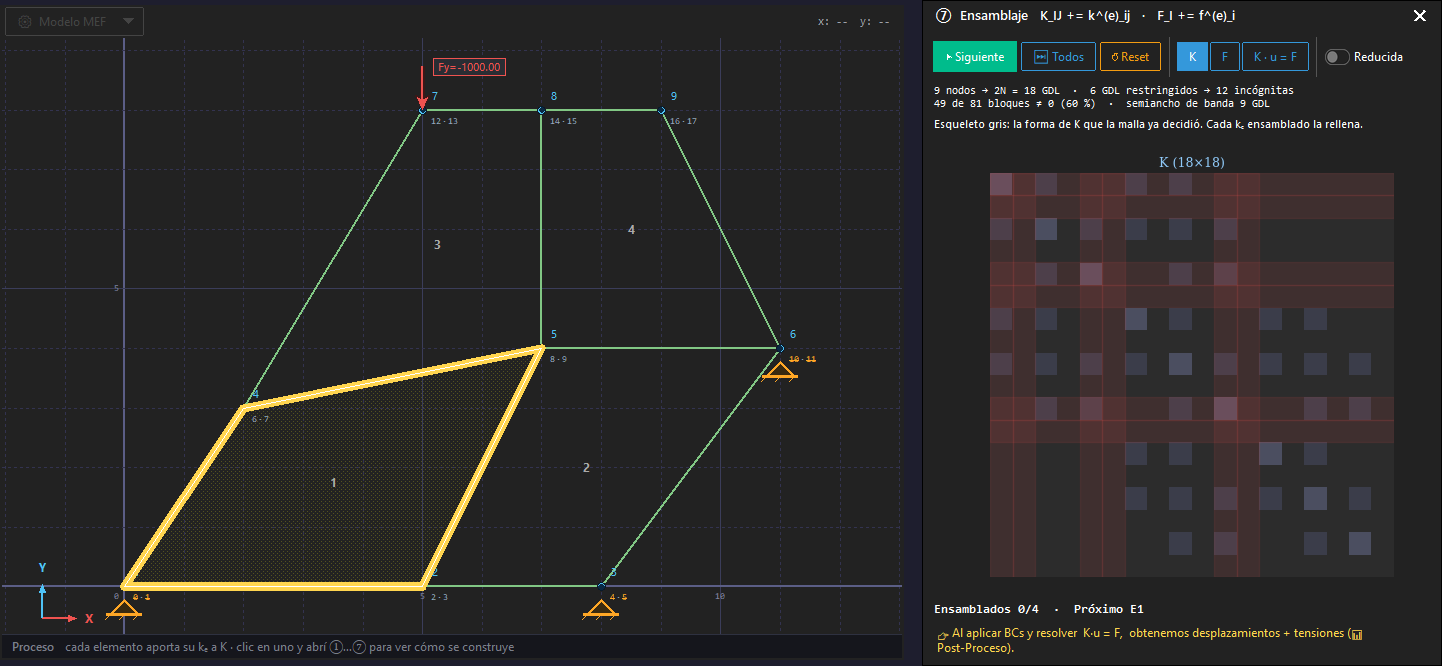
\includegraphics[width=\linewidth]{fig_modulo_m7}
\caption[Módulo M7 (ensamblaje).]{Módulo M7 (ensamblaje). El esqueleto de la matriz global $\bm{K}$ antes de ensamblar ---los bloques que la malla vuelve no nulos---, con las filas y columnas que recibirá el elemento resaltado; en la cabecera, el recuento de GDL, de incógnitas y de bloques no nulos.}
\label{fig:mod-m7}
\end{figure}

De la \autoref{fig:mod-m7} el rasgo a seguir es la correspondencia entre el elemento resaltado en el lienzo y las filas y columnas de $\bm{K}$ que se iluminan: son las posiciones que recibirán su $\bm{k}_e$. Al ensamblar cada elemento, el esqueleto se rellena con valores, y el patrón de entradas no nulas resultante es el acumulado de todos esos aportes.


\clearpage
\section{Referencia del comprobador de salud}
\label{sec:health-checks}

La \autoref{tab:health-checks} reúne todos los chequeos del comprobador de salud, identificados por su código estable, con su significado y si admiten autocorrección desde el diálogo de salud, agrupados por las tres severidades que describe la \autoref{sec:pre-proceso}.

\begin{longtable}{@{}>{\ttfamily\footnotesize}p{2.8cm} >{\footnotesize}l >{\footnotesize\raggedright\arraybackslash}p{5.4cm} >{\footnotesize}c@{}}
\caption[Chequeos del comprobador de salud del modelo, agrupados por severidad.]{Chequeos que el comprobador de salud aplica al modelo antes de resolver, agrupados por severidad. De cada uno se dan el código estable con que el software lo identifica, su significado y si el diálogo de salud ofrece corrección automática. Los errores críticos detienen la resolución, que solo continúa si el usuario elige \textsf{Resolver de todos modos}; las advertencias, no.}
\label{tab:health-checks}\\
\toprule
\normalfont\textbf{Código} & \textbf{Severidad} & \textbf{Significado} & \textbf{Autocorrección} \\
\midrule
\endfirsthead
\multicolumn{4}{@{}l}{\small (continuación de la \autoref{tab:health-checks})}\\
\toprule
\normalfont\textbf{Código} & \textbf{Severidad} & \textbf{Significado} & \textbf{Autocorrección} \\
\midrule
\endhead
\midrule
\multicolumn{4}{r@{}}{\small continúa en la página siguiente}\\
\endfoot
\bottomrule
\endlastfoot

% --- Errores criticos ---
no\_elements & Error crítico & El modelo no tiene ningún elemento; es preciso agregar al menos uno para poder resolver. & No \\
\addlinespace
elem\_node\_missing & Error crítico & Un elemento referencia en sus \texttt{node\_ids} un nodo que no existe en el modelo. & No \\
\addlinespace
elem\_material\_missing & Error crítico & Un elemento usa un nombre de material que no figura en la librería de materiales. & No \\
\addlinespace
degenerate\_element & Error crítico & Un elemento tiene vértices repetidos (menos de cuatro distintos); su Jacobiano será cero o negativo. & No \\
\addlinespace
non\_positive\_thickness & Error crítico & Un elemento tiene espesor $t \le 0$: con $t = 0$ no aporta rigidez ($\bm{k}_e = \bm{0}$) y con $t < 0$ invierte el signo de $\bm{k}_e$. & No \\
\addlinespace
non\_positive\_young & Error crítico & Un material en uso tiene $E \le 0$: la matriz $\bm{D}$ no representa ningún sólido y $\bm{K}$ queda singular o con rigidez negativa. & No \\
\addlinespace
invalid\_poisson & Error crítico & Un material en uso tiene $\nu$ fuera del intervalo $(-1;\ 0{,}5)$, el rango físico de un material isótropo: fuera de él, la $\bm{D}$ de deformación plana deja de ser definida positiva, y en $\nu = 0{,}5$ su factor $1-2\nu$ se anula. & No \\
\addlinespace
negative\_density & Error crítico & La gravedad está activa y un material en uso tiene densidad negativa: el peso propio $F = \rho\, g\, V$ queda invertido. & No \\
\addlinespace
surface\_node\_missing & Error crítico & Una carga de superficie referencia como extremo (\texttt{node\_start} o \texttt{node\_end}) un nodo inexistente. & Sí \\
\addlinespace
no\_restraints & Error crítico & No hay ninguna restricción definida; el modelo conserva los modos de cuerpo rígido y la matriz de rigidez reducida $\bm{K}$ resulta singular. & No \\
\addlinespace
insufficient\_restraints & Error crítico & Hay menos de tres GDL restringidos; se necesitan al menos tres (dos traslaciones y una rotación rígida en el plano) para suprimir los modos de cuerpo rígido en 2D. & No \\
\addlinespace
bc\_orphan\_node & Error crítico & Un nodo tiene restricción pero no pertenece a ningún elemento: es un GDL colgante restringido, que no actúa sobre la estructura; si el nodo conserva además un GDL libre, el sistema reducido queda singular. & Sí \\
\addlinespace
orphan\_free\_node & Error crítico & Un nodo no pertenece a ningún elemento y tiene al menos un GDL libre: aporta filas y columnas nulas a $\bm{K}$ y el sistema reducido queda singular. & Sí \\
\midrule

% --- Advertencias ---
load\_orphan\_node & Advertencia & Un nodo tiene carga pero no pertenece a ningún elemento: la carga entra en el vector $\bm{F}$, pero el nodo no aporta rigidez, de modo que no actúa sobre la estructura; si el nodo tiene algún GDL libre, el sistema queda además singular (\texttt{orphan\_free\_node}). & Sí \\
\addlinespace
unused\_material & Advertencia & Un material está definido en la librería pero ningún elemento lo utiliza. & Sí \\
\addlinespace
negative\_jacobian & Advertencia & Un elemento tiene los nodos en orden horario (área con signo negativa); su Jacobiano será negativo y debe reordenarse en sentido antihorario. & No \\
\addlinespace
zero\_nodal\_load & Advertencia & Una carga nodal tiene componentes $F_x$ y $F_y$ nulas, probablemente por valores sin asignar. & Sí \\
\addlinespace
zero\_surface\_load & Advertencia & Una carga de superficie tiene $q_{\text{inicio}}$ y $q_{\text{fin}}$ nulas y no contribuye al análisis. & Sí \\
\addlinespace
suspicious\_young\_modulus & Advertencia & El módulo de elasticidad $E$ de un material en uso queda fuera del rango físico típico (de unos \mbox{$100$~MPa} a \mbox{$500$~GPa}); sugiere un posible error de unidades. & No \\
\addlinespace
suspicious\_model\_scale & Advertencia & La extensión del modelo queda fuera del rango habitual (de \mbox{$0{,}1$~mm} a \mbox{$10$~km}); sugiere un posible error en la unidad de longitud. & No \\
\addlinespace
gravity\_no\_density & Advertencia & La gravedad está activa (\texttt{include\_gravity}) pero un material en uso tiene densidad $\rho = 0$, de modo que la fuerza volumétrica $F = \rho\, g\, V$ será nula. & No \\
\midrule

% --- Informacion ---
summary & Información & Contadores generales del modelo: número de nodos, de elementos y de GDL totales, libres y restringidos. & No \\

\end{longtable}



\chapter{Listados de código seleccionados}
\label{anexo:codigo}

Se reproducen aquí fragmentos representativos del motor numérico, escogidos por condensar la formulación isoparamétrica descrita en el \autoref{cap:marco_teorico}. El código completo, incluida la interfaz gráfica y los módulos educativos, está disponible en el repositorio público del proyecto\footnote{Repositorio del proyecto: \url{https://github.com/Sucullani/SoftwareED}}.

El alcance de la transcripción es el siguiente. Las \textbf{líneas ejecutables se copian literalmente del repositorio}: no se han renombrado variables, reordenado instrucciones ni abreviado expresiones, de modo que lo que aquí se lee es lo que el software ejecuta. La única intervención afecta a las cadenas de documentación y a los comentarios, que se han recortado para que cada fragmento entre en la caja de texto: se han suprimido líneas en blanco y algún esquema de numeración de nodos, y en la matriz constitutiva la cadena de documentación se ha reducido a un renglón, compensado con dos comentarios al margen que rotulan cada rama. Los comentarios que se conservan son los del código fuente, con su notación matemática ($\xi$, $\partial$, $\varepsilon$, \dots) compuesta fielmente.

\section{Funciones de forma}

El listado evalúa las funciones de forma del Q4 (bilineal) y del Q9 (bicuadrático lagrangiano) en coordenadas naturales, según la \autoref{eq:N-q4} y la \autoref{eq:N-q9}.

\begin{lstlisting}
def shape_functions_q4(xi, eta):
    """Funciones de forma para elemento Q4 (4 nodos).
    Nodos numerados en sentido antihorario:
      4 ---- 3
      |      |
      1 ---- 2
    Retorna: N = [N1, N2, N3, N4] array (4,)
    """
    N = np.empty(4)
    N[0] = 0.25 * (1.0 - xi) * (1.0 - eta)
    N[1] = 0.25 * (1.0 + xi) * (1.0 - eta)
    N[2] = 0.25 * (1.0 + xi) * (1.0 + eta)
    N[3] = 0.25 * (1.0 - xi) * (1.0 + eta)
    return N


def shape_functions_q9(xi, eta):
    """Funciones de forma para elemento Q9 (9 nodos).
    Retorna: N = [N1, ..., N9] array (9,)
    """
    xi2 = xi * xi
    eta2 = eta * eta
    N = np.empty(9)
    # Nodos esquina
    N[0] = 0.25 * xi * (xi - 1.0) * eta * (eta - 1.0)
    N[1] = 0.25 * xi * (xi + 1.0) * eta * (eta - 1.0)
    N[2] = 0.25 * xi * (xi + 1.0) * eta * (eta + 1.0)
    N[3] = 0.25 * xi * (xi - 1.0) * eta * (eta + 1.0)
    # Nodos de lado
    N[4] = 0.5 * (1.0 - xi2) * eta * (eta - 1.0)
    N[5] = 0.5 * xi * (xi + 1.0) * (1.0 - eta2)
    N[6] = 0.5 * (1.0 - xi2) * eta * (eta + 1.0)
    N[7] = 0.5 * xi * (xi - 1.0) * (1.0 - eta2)
    # Nodo central
    N[8] = (1.0 - xi2) * (1.0 - eta2)
    return N
\end{lstlisting}

\section{Matriz de deformación-desplazamiento \texorpdfstring{$\bm{B}$}{B}}

Construye $\bm{B}$ ($3\times 2n$), con la estructura de la \autoref{eq:matriz-B}, a partir de las derivadas físicas de las funciones de forma: es la relación $\bm{\varepsilon} = \bm{B}\,\bm{u}_e$.

\begin{lstlisting}
def compute_b_matrix(dN_phys):
    """Construye la matriz B a partir de las derivadas físicas de N.

    B = [[∂N1/∂x,   0,     ∂N2/∂x,   0,     ...],
         [  0,    ∂N1/∂y,    0,     ∂N2/∂y,  ...],
         [∂N1/∂y, ∂N1/∂x,  ∂N2/∂y, ∂N2/∂x,  ...]]
    Parámetros:
        dN_phys: array (2, n_nodes) - [∂N/∂x; ∂N/∂y]
    Retorna:
        B: array (3, 2*n_nodes)
    """
    n_nodes = dN_phys.shape[1]
    B = np.zeros((3, 2 * n_nodes))
    for i in range(n_nodes):
        B[0, 2 * i] = dN_phys[0, i]       # ∂Ni/∂x → εx
        B[1, 2 * i + 1] = dN_phys[1, i]   # ∂Ni/∂y → εy
        B[2, 2 * i] = dN_phys[1, i]       # ∂Ni/∂y → γxy
        B[2, 2 * i + 1] = dN_phys[0, i]   # ∂Ni/∂x → γxy
    return B
\end{lstlisting}

\section{Matriz constitutiva \texorpdfstring{$\bm{D}$}{D}}

Relaciona tensiones y deformaciones, $\bm{\sigma} = \bm{D}\,\bm{\varepsilon}$, con las dos variantes de elasticidad plana de la \autoref{eq:D-tension-plana} y la \autoref{eq:D-deformacion-plana}.

\begin{lstlisting}
def constitutive_matrix(E, nu, analysis_type):
    """Tensión plana (σz = 0) o deformación plana (εz = 0)."""
    D = np.zeros((3, 3))
    if analysis_type == ANALYSIS_PLANE_STRESS:   # Tensión plana
        factor = E / (1.0 - nu * nu)
        D[0, 0] = factor
        D[0, 1] = factor * nu
        D[1, 0] = factor * nu
        D[1, 1] = factor
        D[2, 2] = factor * (1.0 - nu) / 2.0
    elif analysis_type == ANALYSIS_PLANE_STRAIN: # Deformación plana
        factor = E / ((1.0 + nu) * (1.0 - 2.0 * nu))
        D[0, 0] = factor * (1.0 - nu)
        D[0, 1] = factor * nu
        D[1, 0] = factor * nu
        D[1, 1] = factor * (1.0 - nu)
        D[2, 2] = factor * (1.0 - 2.0 * nu) / 2.0
    else:
        raise ValueError(f"Tipo de análisis no reconocido: {analysis_type}")
    return D
\end{lstlisting}

\section{Ensamblaje disperso de la matriz de rigidez global}

Es el núcleo de la escalabilidad analizada en el \autoref{cap:resultados}. El arreglo \texttt{dofs} ($e\times 2n$) reúne los GDL globales de cada elemento, obtenidos vía \texttt{node\_index\_map}, y \texttt{ke} ($e\times 2n\times 2n$), sus rigideces, calculadas de una vez por lotes. Cada entrada $k_e[i,j]$ se dispersa a $K[g_i, g_j]$ según el operador de la \autoref{eq:ensamblaje} (el \emph{scatter} local $\to$ global), por tripletes COO, convertidos a filas comprimidas CSR para el solucionador disperso.

\begin{lstlisting}
def assemble_sparse(dofs, ke, n_dof):
    """Scatter local -> global como tripletes COO y conversion a CSR.

    `coo_matrix` suma las entradas duplicadas en la misma (i, j): es
    exactamente la suma de contribuciones elementales del MEF. K nunca se
    materializa densa (memoria O(nnz)).
    """
    dofs = np.asarray(dofs, dtype=np.intp)
    n_dof_e = dofs.shape[1] if dofs.ndim == 2 else 0
    rows = np.repeat(dofs, n_dof_e, axis=1).ravel()   # [i0, i0, ..., i1, i1, ...]
    cols = np.tile(dofs, (1, n_dof_e)).ravel()        # [j0, j1, ..., j0, j1, ...]
    data = np.asarray(ke, dtype=float).ravel()
    return coo_matrix((data, (rows, cols)), shape=(n_dof, n_dof)).tocsr()
\end{lstlisting}


\chapter{Resultados extendidos de verificación y validación}
\label{anexo:vyv}

Este anexo amplía la evidencia del \autoref{cap:resultados} con tablas y figuras complementarias, generadas por los mismos guiones de verificación y validación del proyecto, salvo la captura de la \autoref{fig:cook-def}. Los datos crudos se conservan en los archivos CSV del directorio \texttt{docs/vyv/datos/} del repositorio, con los que pueden cotejarse las cifras reportadas aun sin volver a ejecutar el código.

\section{Reproducibilidad de la verificación y validación}
\label{sec:vyv-reproducibilidad}

Toda la evidencia numérica del \autoref{cap:resultados} y de este anexo se genera con los guiones de verificación y validación incluidos en el repositorio del proyecto. El conjunto de pruebas no se apoya en un marco de pruebas automatizado del tipo \texttt{pytest}: cada guion se ejecuta por sí solo como módulo de Python e imprime su diagnóstico por consola. Los tres guiones de verificación y validación depositan además los datos crudos, en archivos CSV, en \texttt{docs/vyv/datos/}, y las figuras en \texttt{docs/vyv/figuras/}. La organización es determinista y reejecutable: basta volver a lanzar el comando correspondiente para regenerar la tabla o la figura asociada, y cada cifra reportada puede repetirse. Los comandos se invocan desde la raíz del proyecto, con el entorno virtual activado y las dependencias instaladas según el \autoref{anexo:instalacion}. La \autoref{tab:vyv-repro} enumera los siete guiones que producen o sostienen esa evidencia, indica qué verifica o valida cada uno y remite a la tabla o figura concreta que le corresponde, tanto en el cuerpo principal como en este anexo.

% longtable y no table+tabular: la tabla mide mas que una hoja y como flotante
% la ultima fila salia cortada por el borde inferior ("Float too large for page").
{\setlength{\tabcolsep}{4pt}
\begin{longtable}{@{}>{\footnotesize\raggedright\arraybackslash}p{4.3cm} >{\footnotesize\raggedright\arraybackslash}p{5.1cm} >{\footnotesize\raggedright\arraybackslash}p{4.1cm}@{}}
\caption[Guía de reproducibilidad de la batería de verificación y validación.]{Guía de reproducibilidad de la batería de verificación y validación: comando de ejecución de cada guion, objeto de la prueba y resultados asociados en el \autoref{cap:resultados} y en este anexo.}
\label{tab:vyv-repro}\\
\toprule
\textbf{Guion} & \textbf{Qué verifica} & \textbf{Resultados (Capítulo 3 / Anexo)} \\
\midrule
\endfirsthead
\multicolumn{3}{@{}l}{\small (continuación de la \autoref{tab:vyv-repro})}\\
\toprule
\textbf{Guion} & \textbf{Qué verifica} & \textbf{Resultados (Capítulo 3 / Anexo)} \\
\midrule
\endhead
\midrule
\multicolumn{3}{r@{}}{\small continúa en la página siguiente}\\
\endfoot
\bottomrule
\endlastfoot
\texttt{python -m}\newline\texttt{tests.vv\_mms} &
Verificación por el método de soluciones manufacturadas: tasas asintóticas de convergencia en norma $L^2$ y seminorma $H^1$ del desplazamiento y en norma $L^2$ del campo de tensiones recuperado, para Q4 y Q9, en cuatro configuraciones (cuadrado unitario y cuadrilátero distorsionado, tensión y deformación plana). &
\autoref{tab:mms}, \autoref{fig:convergencia}, \autoref{fig:convergencia-tension}, \autoref{tab:mms-rel}, \autoref{tab:mms-configs}, \autoref{fig:mms-campos} \\
\addlinespace
\texttt{python -m}\newline\texttt{tests.vv\_timoshenko} &
Validación de la viga simplemente apoyada frente a la solución analítica de Timoshenko-Goodier y al modelo de cáscara de SAP2000: tensión normal $\sigma_x$, componentes $\sigma_y$ y $\tau_{xy}$, desplazamientos, deflexión máxima y equilibrio global de reacciones. &
\autoref{tab:timoshenko-stress}, \autoref{tab:timoshenko-defl}, \autoref{tab:tim-componentes}, \autoref{tab:tim-desp}, \autoref{fig:tim-perfil} \\
\addlinespace
\texttt{python -m}\newline\texttt{tests.vv\_cook} &
Validación con la membrana de Cook: convergencia del desplazamiento $u_y$ en $(48;\ 52)$ bajo refinamiento, evidenciando el bloqueo por cortante del Q4 frente a la convergencia del Q9. &
\autoref{tab:cook}, \autoref{fig:cook-convergencia}, \autoref{tab:resumen-q4q9}, \autoref{tab:cook-ux} \\
\addlinespace
\texttt{python -m}\newline\texttt{tests.test\_fem} &
Comprobación del motor con los datos de ejemplo, para Q4 y Q9: resolución del sistema $\bm{K}\,\bm{u}=\bm{F}$ con desplazamientos finitos y equilibrio global de las reacciones, y fuerzas nodales equivalentes de una carga superficial. Imprime además las tensiones nodales promedio y la calidad de malla, sin compararlas con valores de referencia. &
Consistencia interna del motor \\
\addlinespace
\texttt{python -m}\newline\texttt{tests.test\_vv\_extensions} &
Regresión de las extensiones del solucionador usadas en la batería de verificación y validación: fuerza de volumen (\texttt{body\_force\_fn}), restricciones de Dirichlet no homogéneas (\texttt{ux\_value}/\texttt{uy\_value}), malla estructurada (\texttt{generate\_structured\_quad\_mesh}) y normas de error $L^2$/$H^1$. Comprueba además que la matriz de extrapolación reproduce exactamente los campos de su espacio de interpolación y, en un estado de deformación uniaxial con solución cerrada, que la tensión de von Mises de la deformación plana coincide con su valor exacto: incluye $\sigma_z$ y depende de los términos $D_{11}$ y $D_{12}$ de su matriz, no de $D_{33}$. &
Soporte de la verificación por soluciones manufacturadas; \autoref{sec:mms}; \autoref{sec:leccion-extrapolacion} \\
\addlinespace
\texttt{python -m}\newline\texttt{tests.test\_interop} &
Intercambio de datos (criterio de la cláusula (a)): ida y vuelta CSV/ZIP del ejemplo guía sin pérdida de entidades y con desplazamientos idénticos; importación del DXF de ejemplo (seis cuadriláteros y doce nodos, con los vértices comunes compartidos; orientación antihoraria) e idempotencia de la reimportación. &
\autoref{sec:consistencia-interna} \\
\addlinespace
\texttt{python -m}\newline\texttt{tests.test\_q9\_q4\_cycle} &
Regresión del ciclo de transformación de malla $\text{Q4}\rightarrow\text{Q9}\rightarrow\text{Q4}$: el campo de desplazamientos de la malla Q4 reducida coincide con el de la Q4 original sin deriva numérica. &
\autoref{sec:consistencia-interna} \\
\end{longtable}}

La \autoref{fig:timoshenko-contorno} y la \autoref{fig:cook-def} no salen de estos guiones: son capturas del post-proceso de EduFEM sobre los mismos casos, y volver a ejecutar los comandos no las regenera. Otros tres guiones sostienen las pruebas que cita la \autoref{sec:consistencia-interna} (\texttt{tests.test\_noncontiguous\_ids}, \texttt{tests.test\_serialization} y \texttt{tests.test\_memoria\_calculo}), y \texttt{tests.bench\_timing} produce la \autoref{tab:tiempos}; todos se ejecutan con la misma orden. Esos guiones forman parte de una batería mayor. En la versión evaluada (\autoref{sec:proceso-met}), la carpeta \texttt{tests/} reúne 36 guiones de prueba, que se reparten así según el componente que ejercitan:

\begin{itemize}
    \item el motor numérico: los tres de verificación y validación y cinco de regresión;
    \item el modelo del proyecto: seis;
    \item la entrada y salida de datos y la memoria de cálculo: tres;
    \item los módulos educativos: tres;
    \item la interfaz gráfica: quince;
    \item el instalador y el arranque del programa: uno.
\end{itemize}

El dato es un recuento de guiones y no una medida de la cobertura del código: dice qué componentes tienen pruebas de regresión, no qué fracción de sus líneas ejecutan.

\section{Método de soluciones manufacturadas: errores relativos y campos}

Además de las normas absolutas reportadas en el cuerpo principal, la \autoref{tab:mms-rel} presenta los errores \emph{relativos} en norma $L^2$ y seminorma $H^1$ de la configuración base, que confirman la misma jerarquía de convergencia con independencia de la escala del problema. Las normas se integraron con un punto de Gauss más por dirección que la rigidez, por la razón que expone la \autoref{sec:verificacion-validacion}. La \autoref{tab:mms-configs} resume las tasas asintóticas ---entre las mallas $N=16$ y $N=32$--- y los errores relativos finales en las cuatro configuraciones: las tasas del desplazamiento coinciden con las teóricas en todas ellas, y las del campo de tensiones recuperado se mantienen en $\mathcal{O}(h^{1{,}5})$ para Q4 y $\mathcal{O}(h^{2})$ para Q9 con independencia del estado plano y de la distorsión de los elementos. Los datos completos se conservan en \texttt{mms\_q4.csv} y \texttt{mms\_q9.csv}, para la configuración base, y en \texttt{mms\_\{q4,q9\}\_\{dist\_tp,unif\_dp,dist\_dp\}.csv}, para las otras tres; el resumen, en \texttt{mms\_resumen.csv}.

\begin{table}[htbp]
\centering
\caption[Errores relativos del MMS en norma $L^2$ y seminorma $H^1$ del desplazamiento.]{Errores relativos del método de soluciones manufacturadas en norma $L^2$ y seminorma $H^1$ del desplazamiento, para Q4 y Q9 en la configuración base, según el número $N$ de elementos por lado. Cada columna debe leerse verticalmente: al duplicar $N$, el error cae en la proporción que fija la tasa de convergencia del elemento.}
\label{tab:mms-rel}
\begin{tabular}{c r r r r}
\hline
 & \multicolumn{2}{c}{\textbf{Q4}} & \multicolumn{2}{c}{\textbf{Q9}} \\
$N$ & $L^2$ rel. & $H^1$ rel. & $L^2$ rel. & $H^1$ rel. \\
\hline
2  & $3{,}619\times10^{-1}$ & $4{,}761\times10^{-1}$ & $3{,}071\times10^{-2}$ & $9{,}267\times10^{-2}$ \\
4  & $1{,}024\times10^{-1}$ & $2{,}307\times10^{-1}$ & $3{,}926\times10^{-3}$ & $2{,}312\times10^{-2}$ \\
8  & $2{,}638\times10^{-2}$ & $1{,}139\times10^{-1}$ & $4{,}921\times10^{-4}$ & $5{,}758\times10^{-3}$ \\
16 & $6{,}645\times10^{-3}$ & $5{,}675\times10^{-2}$ & $6{,}155\times10^{-5}$ & $1{,}438\times10^{-3}$ \\
32 & $1{,}664\times10^{-3}$ & $2{,}835\times10^{-2}$ & $7{,}695\times10^{-6}$ & $3{,}592\times10^{-4}$ \\
\hline
\end{tabular}
\end{table}

\begin{table}[htbp]
\centering
\caption[Tasas asintóticas del MMS en las cuatro configuraciones.]{Tasas asintóticas de convergencia (entre las mallas $N=16$ y $N=32$) y errores relativos en la malla más fina del MMS en las cuatro configuraciones: cuadrado unitario y cuadrilátero distorsionado, en tensión plana (TP) y deformación plana (DP). $\sigma^*$ abrevia el campo de tensiones recuperado $\bm{\sigma}^*_h$. Fuente: \texttt{mms\_resumen.csv}.}
\label{tab:mms-configs}
\small
\setlength{\tabcolsep}{4pt}
\begin{tabular}{l c c c c c r r}
\hline
Dominio & Estado & Elem. & tasa $L^2$ & tasa $H^1$ & tasa $\sigma^*$ & $L^2$ rel. & $\sigma^*$ rel. \\
\hline
Unitario      & TP & Q4 & 1,997 & 1,001 & 1,541 & $1{,}664\times10^{-3}$ & $1{,}156\times10^{-2}$ \\
Unitario      & TP & Q9 & 3,000 & 2,001 & 1,999 & $7{,}695\times10^{-6}$ & $5{,}650\times10^{-4}$ \\
Distorsionado & TP & Q4 & 1,997 & 1,001 & 1,546 & $1{,}325\times10^{-3}$ & $9{,}497\times10^{-3}$ \\
Distorsionado & TP & Q9 & 3,000 & 2,000 & 1,999 & $5{,}733\times10^{-6}$ & $4{,}837\times10^{-4}$ \\
Unitario      & DP & Q4 & 1,997 & 1,002 & 1,530 & $1{,}745\times10^{-3}$ & $1{,}433\times10^{-2}$ \\
Unitario      & DP & Q9 & 3,000 & 2,001 & 1,999 & $7{,}696\times10^{-6}$ & $7{,}069\times10^{-4}$ \\
Distorsionado & DP & Q4 & 1,997 & 1,001 & 1,535 & $1{,}377\times10^{-3}$ & $1{,}177\times10^{-2}$ \\
Distorsionado & DP & Q9 & 3,000 & 2,001 & 1,999 & $5{,}734\times10^{-6}$ & $6{,}038\times10^{-4}$ \\
\hline
\end{tabular}
\end{table}

La \autoref{fig:mms-campos} muestra los campos discretos de desplazamiento sobre la malla Q9 con $N=16$, visualmente indistinguibles de la solución manufacturada de la \autoref{eq:mms-solucion}.

\begin{figure}[htbp]
\centering
\begin{minipage}{0.49\linewidth}
  \centering
  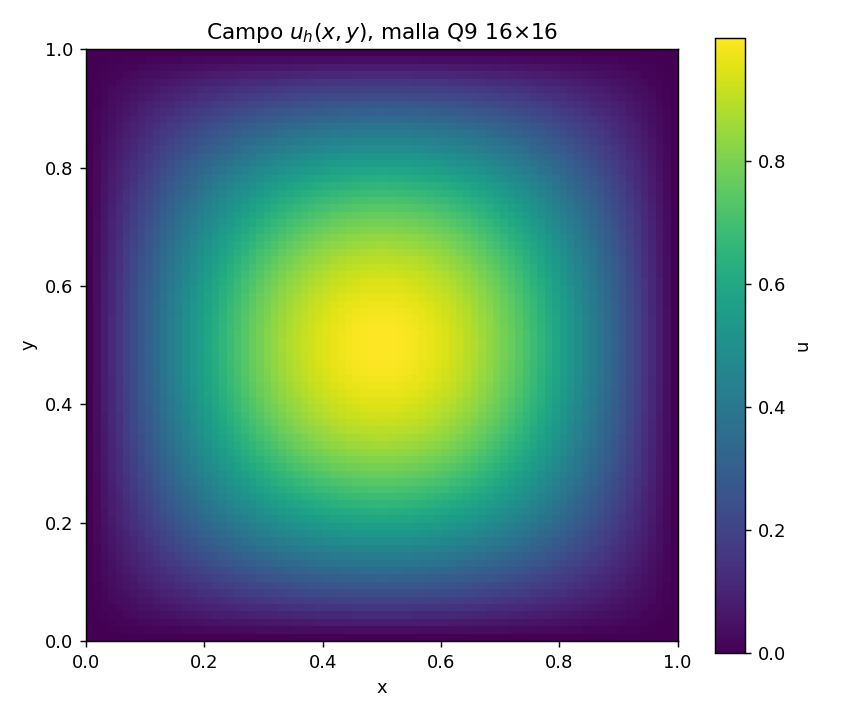
\includegraphics[width=\linewidth]{mms_field_u.png}\\[2pt]
  {\small (a) Componente $u_h(x,y)$.}
\end{minipage}
\hfill
\begin{minipage}{0.49\linewidth}
  \centering
  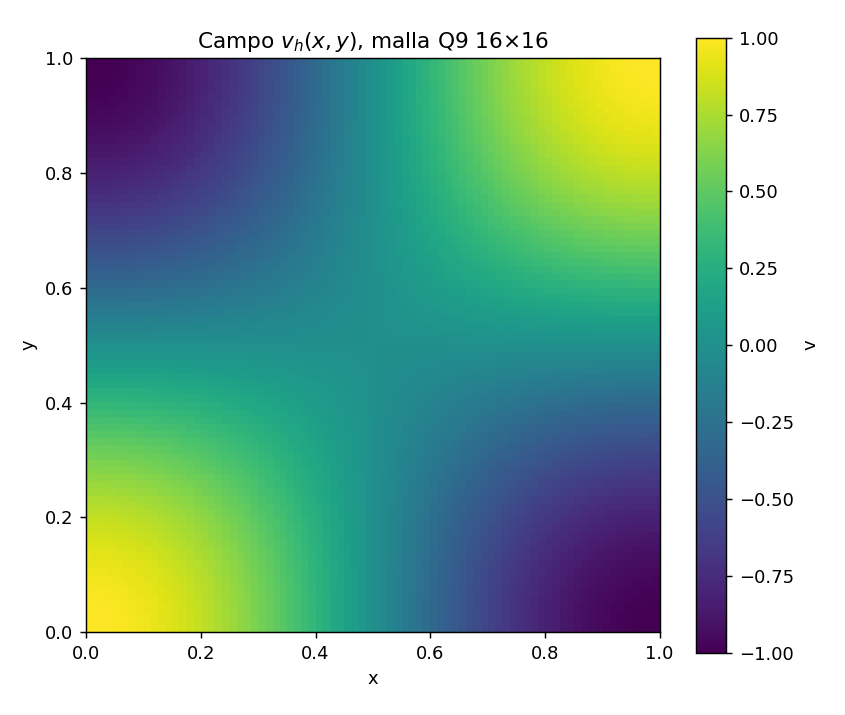
\includegraphics[width=\linewidth]{mms_field_v.png}\\[2pt]
  {\small (b) Componente $v_h(x,y)$.}
\end{minipage}
\caption[Campos discretos $\bm{u}_h$ sobre la malla Q9 con $N=16$.]{Campos discretos de desplazamiento $\bm{u}_h$ calculados sobre la malla Q9 con $N=16$ (2178 GDL) en la verificación por soluciones manufacturadas: (a) la componente horizontal y (b) la vertical. Ambas se leen como la contraparte numérica de la solución manufacturada de la \autoref{eq:mms-solucion}, de la que resultan visualmente indistinguibles.}
\label{fig:mms-campos}
\end{figure}

\section{Viga de Timoshenko: componentes restantes y desplazamientos}

El cuerpo principal contrastó la tensión normal $\sigma_x$. El modelo de SAP2000 y la resolución analítica que originan las referencias de esta sección se reproducen, como evidencia documental, en el \autoref{anexo:sap2000}. La \autoref{tab:tim-componentes} completa el estado tensional con las componentes $\sigma_y$ y $\tau_{xy}$ en los tres puntos de control, junto con su error relativo frente a la solución analítica. Sus dos filas del punto B repiten los valores de la \autoref{tab:timoshenko-stress}, salvo que aquí el $\tau_{xy}$ de SAP2000 conserva su signo original; se reproducen para que el estado tensional pueda leerse completo en un solo cuadro. En estas componentes secundarias la concordancia es, en general, peor que en $\sigma_x$. En el punto B, el error llega al $2{,}89\,\%$ en $\tau_{xy}$ y al $0{,}94\,\%$ en $\sigma_y$, frente al $0{,}04\,\%$ de $\sigma_x$; en el punto C, $\tau_{xy}$ llega al $1{,}00\,\%$, mientras que $\sigma_y$ se queda en el mismo $0{,}03\,\%$ que $\sigma_x$. En el punto A ---donde la solución analítica de ambas componentes es nula--- el error relativo no está definido, y EduFEM devuelve residuos de $0{,}0138$ y $0{,}0000$~kgf/cm$^2$. La razón es de escala (\autoref{sec:interpretacion}): estas componentes son entre seis y treinta y cinco veces más pequeñas que $\sigma_x$, de modo que un error absoluto del mismo orden pesa mucho más en términos relativos. En $\tau_{xy}$ se suma que su error absoluto es entre cinco y diez veces el de $\sigma_x$.

En $\tau_{xy}$ el modelo de SAP2000 queda, en valor absoluto, más cerca de la solución analítica ($0{,}16\,\%$ en B, según los valores de la \autoref{tab:tim-componentes}) que EduFEM. La diferencia de signo en $\tau_{xy}$ frente a SAP2000 proviene de la convención de eje $y$ (la solución de Timoshenko-Goodier emplea $y$ hacia abajo, y el guion de validación aplica el cambio $y_{\text{MEF}} = -y_{\text{ref}}$, que invierte el signo de las componentes sensibles a la reflexión).

\begin{table}[htbp]
\centering
\caption[Componentes $\sigma_y$ y $\tau_{xy}$ en los puntos de control de la viga de Timoshenko.]{Componentes $\sigma_y$ y $\tau_{xy}$ (kgf/cm$^2$) en los puntos de control de la viga de Timoshenko y error relativo de EduFEM frente a la solución analítica. En el punto A la solución analítica de ambas componentes es nula, de modo que el error relativo no está definido y la celda lleva una raya.}
\label{tab:tim-componentes}
\begin{tabular}{c c r r r c}
\hline
Punto & Componente & EduFEM & Analítico & SAP2000 & Error anal.\ (\%) \\
\hline
A & $\sigma_y$  & $0{,}0138$  & $0{,}0000$  & $-0{,}0790$ & --- \\
A & $\tau_{xy}$ & $0{,}0000$  & $0{,}0000$  & $0{,}0000$  & --- \\
B & $\sigma_y$  & $-1{,}0646$ & $-1{,}0547$ & $-1{,}0182$ & 0,94 \\
B & $\tau_{xy}$ & $5{,}4257$  & $5{,}2734$  & $-5{,}2818$ & 2,89 \\
C & $\sigma_y$  & $-0{,}9256$ & $-0{,}9259$ & $-0{,}9054$ & 0,03 \\
C & $\tau_{xy}$ & $4{,}9096$  & $4{,}8611$  & $-4{,}8774$ & 1,00 \\
\hline
\end{tabular}
\end{table}

La \autoref{tab:tim-desp} compara los desplazamientos horizontal y vertical en los mismos puntos frente a SAP2000, con diferencias de hasta el $0{,}56\,\%$ en la componente vertical.

\begin{table}[htbp]
\centering
\caption{Desplazamientos $u_x$ y $u_y$ (cm) en los puntos de control: EduFEM frente a SAP2000.}
\label{tab:tim-desp}
\begin{tabular}{c r r r r c}
\hline
Punto & $u_x$ EduFEM & $u_y$ EduFEM & $u_x$ SAP2000 & $u_y$ SAP2000 & Difer.\ $u_y$ (\%) \\
\hline
A & $0{,}00040$ & $2{,}03101$ & $0{,}0000$ & $2{,}0231$ & 0,39 \\
B & $0{,}11363$ & $1{,}09871$ & $0{,}1133$ & $1{,}0926$ & 0,56 \\
C & $0{,}06272$ & $1{,}45216$ & $0{,}0624$ & $1{,}4453$ & 0,47 \\
\hline
\end{tabular}
\end{table}

La \autoref{fig:tim-perfil} muestra el perfil de $\sigma_x$ a lo largo del peralte en el centro del vano: los valores de EduFEM siguen la solución analítica de Timoshenko-Goodier, trazada en la misma figura, y en la fibra extrema reproducen el valor del punto A de la \autoref{tab:timoshenko-stress}.

\begin{figure}[!htb]
\centering
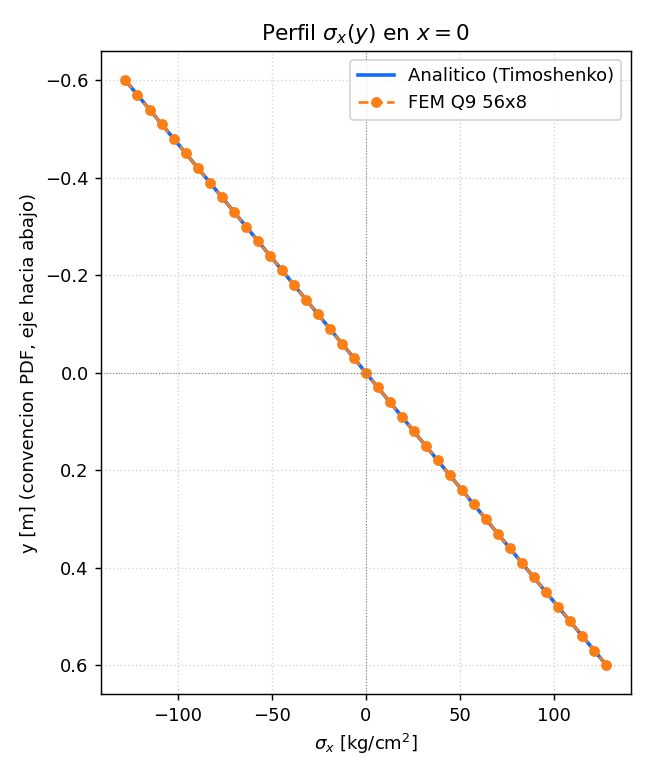
\includegraphics[width=0.5\linewidth]{timoshenko_perfil_x0.png}
\caption[Perfil de $\sigma_x$ en el centro del vano de la viga de Timoshenko.]{Perfil de $\sigma_x(y)$ en $x=0$ (centro del vano) de la viga de Timoshenko: solución analítica de Timoshenko-Goodier y valores de EduFEM sobre la malla Q9. El eje $y$ apunta hacia abajo, como en la solución de referencia. La distribución es prácticamente lineal en el peralte, coherente con la teoría de vigas.}
\label{fig:tim-perfil}
\end{figure}

\section{Membrana de Cook: desplazamiento horizontal y deformada}

La cantidad de interés del cuerpo principal fue el desplazamiento vertical $u_y$. La \autoref{tab:cook-ux} reporta el desplazamiento horizontal $u_x$ en el mismo punto $(48;\ 52)$, que converge igualmente y con mayor rapidez para el Q9. La \autoref{fig:cook-def} ilustra la configuración deformada para la malla Q9 con $N=8$.

\begin{table}[htbp]
\centering
\caption[Desplazamiento horizontal $u_x$ en $(48;\ 52)$ de la membrana de Cook.]{Desplazamiento horizontal $u_x$ en el punto $(48;\ 52)$ de la membrana de Cook, para Q4 y Q9, según el número $N$ de elementos por lado. Se lee por columna: el Q9 alcanza su valor convergido con mallas mucho más gruesas que el Q4.}
\label{tab:cook-ux}
\begin{tabular}{c r r}
\hline
$N$ & $u_x$ (Q4) & $u_x$ (Q9) \\
\hline
2  & $-4{,}091$  & $-10{,}362$ \\
4  & $-7{,}661$  & $-10{,}640$ \\
8  & $-9{,}713$  & $-10{,}673$ \\
16 & $-10{,}422$ & $-10{,}685$ \\
32 & $-10{,}619$ & $-10{,}691$ \\
\hline
\end{tabular}
\end{table}

\begin{figure}[!htb]
\centering
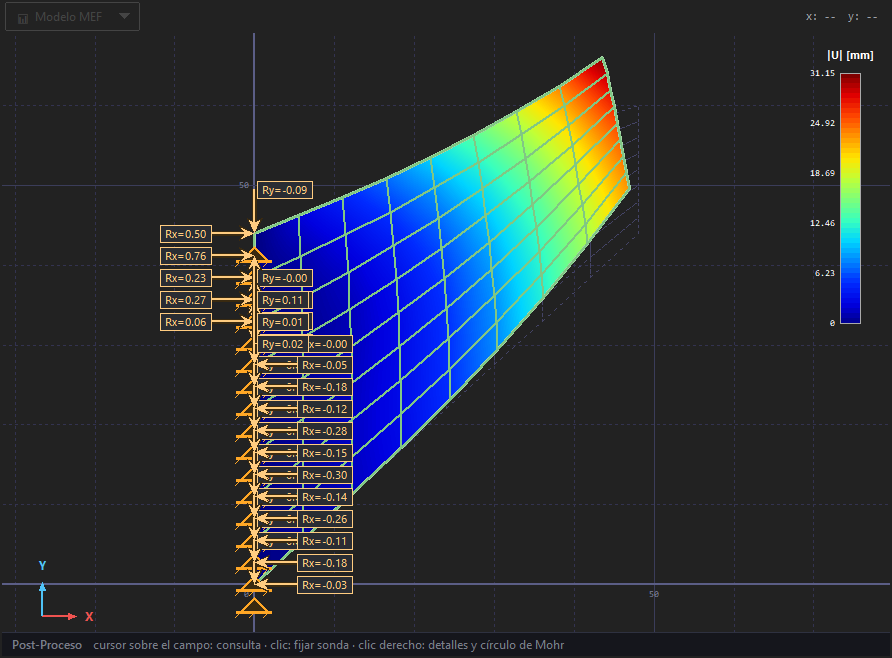
\includegraphics[width=0.78\linewidth]{figuras/fig_cook_deformed}
\caption[Deformada de la membrana de Cook (Q9, $N=8$).]{Post-proceso de EduFEM: configuración deformada de la membrana de Cook (Q9, $N=8$) con el contorno de magnitud de desplazamiento $|U|$. El empotramiento del borde izquierdo y el desplazamiento creciente hacia el extremo libre cargado son visibles sobre la geometría original (en línea punteada).}
\label{fig:cook-def}
\end{figure}


\chapter{Modelo en SAP2000 y solución analítica de Timoshenko}
\label{anexo:sap2000}

Las páginas que siguen son la verificación del caso de la viga realizada con SAP2000, elaborada por el autor, de la que provienen las cifras de contraste que el \autoref{cap:resultados} compara con EduFEM y que el \autoref{anexo:vyv} amplía. El documento reúne la resolución analítica de las tensiones $\sigma_x$, $\sigma_y$ y $\tau_{xy}$ y de los desplazamientos según la teoría de la elasticidad de Timoshenko-Goodier \autocite[art.~21, pp.~39-43]{timoshenko1970elasticity} y el modelado de la misma viga en SAP2000 \autocite[p.~179]{csi2017sap2000} con elementos de cáscara (\emph{shell}). Añade la comparación numérica punto a punto entre ambas referencias en los puntos A, B y C, y el contraste de la deflexión por teoría de vigas, con y sin corrección por cortante. Se incorpora como evidencia documental para dar trazabilidad a esas cifras; sus hojas apaisadas se presentan giradas sobre la hoja vertical, con el folio de la tesis.

Se reproduce tal como fue elaborado, sin rehacer su composición, y por eso conserva convenciones propias, distintas de las del resto del documento. Las principales son cuatro:

\begin{itemize}
    \item escribe «esfuerzo» donde esta tesis escribe «tensión», con el mismo significado;
    \item emplea el punto como separador decimal, frente a la coma del cuerpo y de las tablas del \autoref{anexo:vyv};
    \item expresa las tensiones en kg/cm$^2$, unidad que aquí se escribe kgf/cm$^2$;
    \item usa rótulos y símbolos propios.
\end{itemize}

El peralte $H$, la luz $L$, la base $b$ y la carga distribuida $q$ tienen el significado que les da la Nomenclatura; los demás símbolos del documento no figuran en ella:

\begin{itemize}
    \item $f'_c$, la resistencia característica del hormigón, y $f_y$, el límite de fluencia del acero;
    \item $c = H/2$, el semiperalte, y $l = L/2$, la semiluz;
    \item $I$, el momento de inercia;
    \item $v$, el coeficiente de Poisson, que el cuerpo denota $\nu$.
\end{itemize}

Se conserva además su estilo tipográfico y ortográfico original —títulos en mayúsculas sin tilde, abreviaturas propias y erratas de digitación, como «SAP200», «poison» o «Dezplazamiento»—, junto con las capturas en la resolución en que fueron tomadas.

Dos lecturas del documento requieren una acotación. La primera: la comprobación de que ninguna tensión supera $f'_c = 210$~kgf/cm$^2$ es una lectura de admisibilidad del material, ajena al alcance de este trabajo, que es elástico lineal y no evalúa la capacidad de la sección; otro tanto ocurre con el límite de fluencia del acero de la primera hoja, que no interviene en el análisis. La segunda: en la hoja de discusión de $\sigma_x$, la observación de que en $x = \pm 7$~m «existirá momentos» debe entenderse así: el segundo término de la expresión de Timoshenko-Goodier deja en los apoyos una distribución de $\sigma_x$ autoequilibrada, cuya resultante y cuyo momento son nulos, por lo que el momento flector en los apoyos sigue siendo cero, como corresponde a la viga simplemente apoyada.

% Cada pagina lleva el folio de la tesis. La pag. 1 del original es vertical
% (carta, mas ancha que el A4): lleva la misma escala que las demas para dejarle
% margen de encuadernacion, y el pie completo de la tesis (estilo fancy). Las 2-11
% son apaisadas: se giran 90 grados sobre la hoja vertical (angle=90), como una
% figura apaisada, de modo que el numero de pagina queda en su sitio habitual;
% llevan solo el numero (estilo plain), porque el nombre del capitulo y el filete
% quedarian perpendiculares a su contenido. (Con landscape=true pdfpages usa
% pdflscape y el pie no se imprimia.) final4: sin el offset=0 -12pt de final3,
% que apartaba las hojas del numero cuando iba en el encabezado; scale deja libre
% la franja del pie.
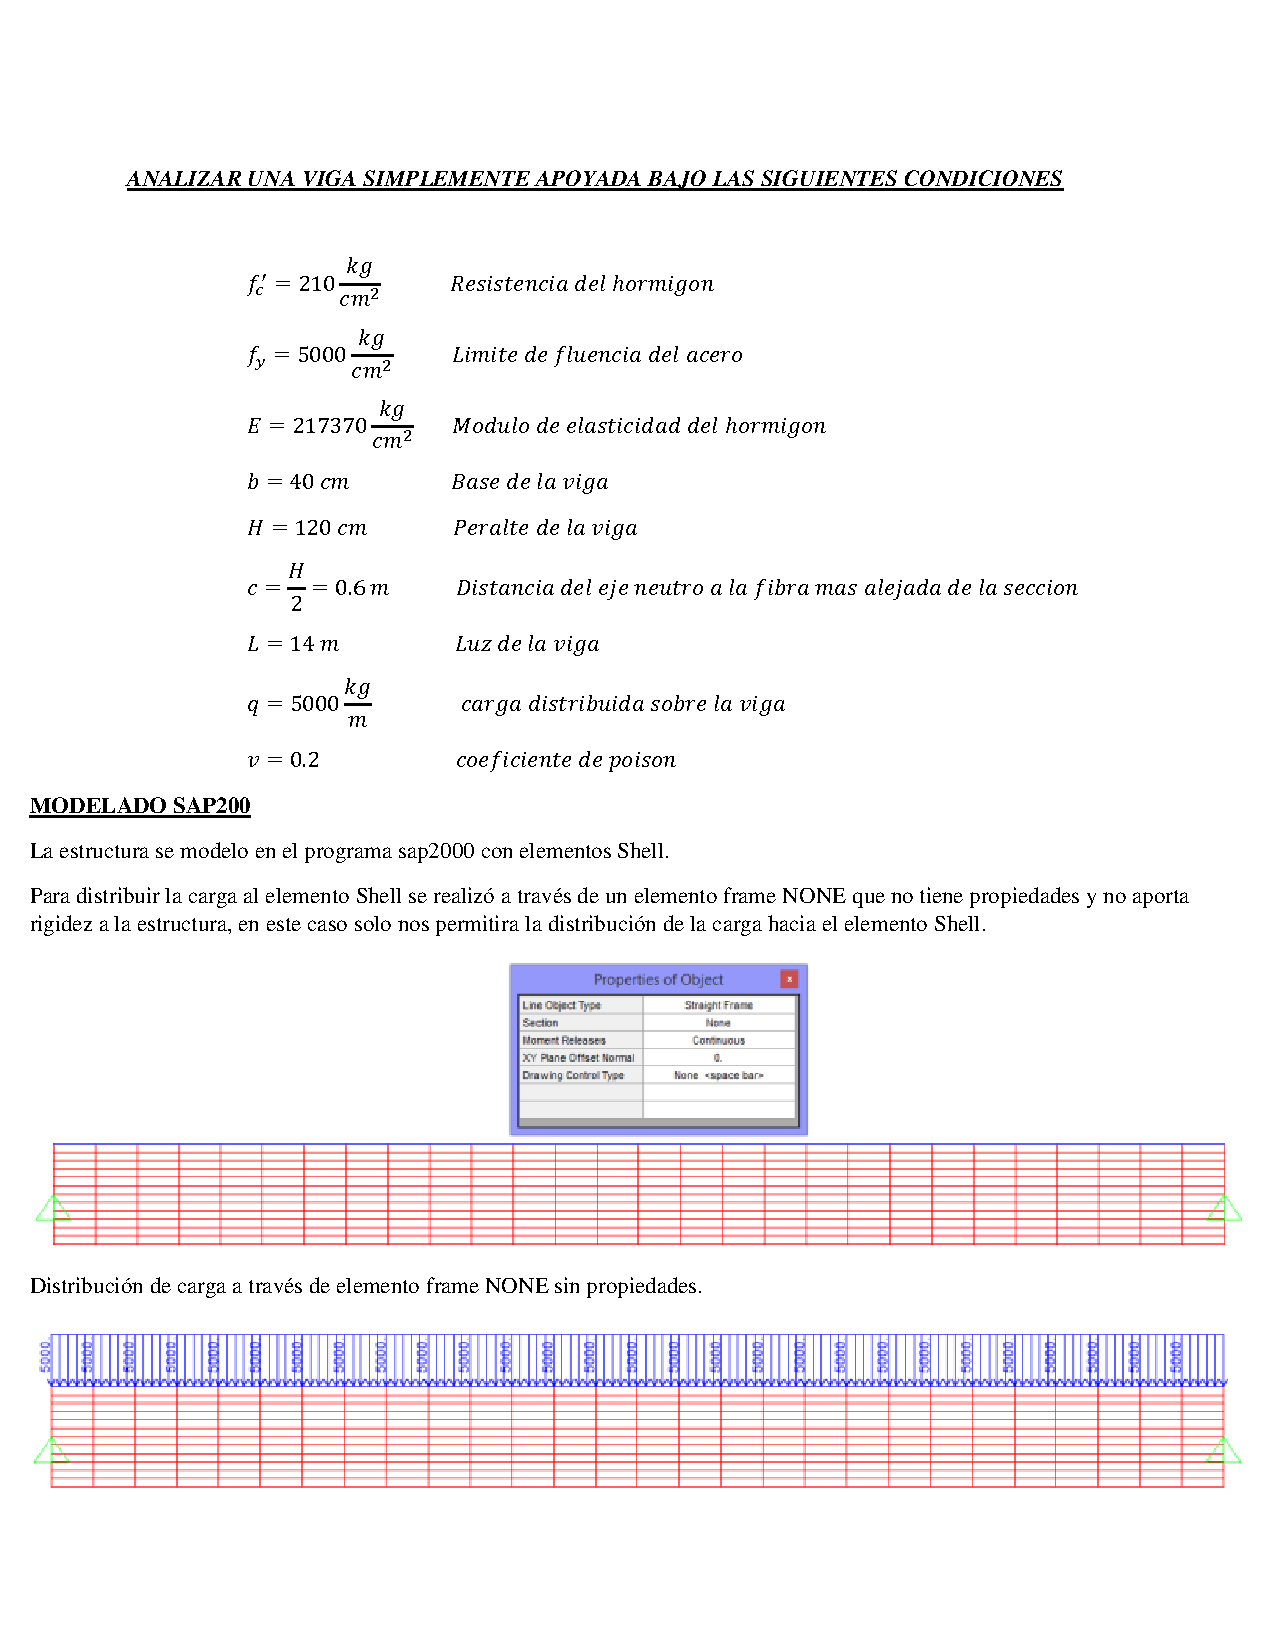
\includepdf[pages=1,scale=0.88,pagecommand={\thispagestyle{fancy}}]{anexos/validacion_sap2000.pdf}
\includepdf[pages=2-11,angle=90,scale=0.88,pagecommand={\thispagestyle{plain}}]{anexos/validacion_sap2000.pdf}


\chapter{Formatos de intercambio de datos}
\label{anexo:formatos}

EduFEM intercambia datos con el exterior mediante tres formatos de archivo, cada uno con un propósito distinto: el formato nativo \texttt{.edufem} para guardar y reabrir el proyecto completo sin pérdida de información; un paquete de archivos CSV comprimido para la edición masiva del modelo en una hoja de cálculo; y el formato DXF de dibujo asistido para importar la geometría desde un programa de diseño. Este anexo documenta, como referencia, la estructura de cada uno tal como la lee y escribe el software.

\section{Proyecto nativo (\texttt{.edufem})}

Un archivo \texttt{.edufem} es un documento de texto en formato JSON, codificado en UTF-8, que almacena la totalidad del modelo ---geometría, propiedades, cargas y restricciones--- pero \emph{no} los resultados del cálculo, que EduFEM recomputa al volver a resolver el modelo (tecla F5 o paso al post-proceso). La serialización la produce el método \texttt{to\_dict} de la clase \texttt{ProjectModel}, y la lectura inversa el método \texttt{from\_dict}; ambos comparten el mismo esquema de claves.

El guardado es \textbf{atómico}: el contenido se escribe primero en un archivo temporal del mismo directorio, se fuerza su descarga a disco (\texttt{fsync}) y solo entonces se renombra sobre el destino final mediante \texttt{os.replace}. De este modo, una interrupción a mitad de escritura ---un cierre forzado, un disco lleno o un corte de energía--- nunca deja el archivo original corrupto o truncado: queda intacto el contenido anterior o bien el nuevo completo. La escritura usa una indentación de dos espacios y conserva los caracteres no ASCII (\texttt{ensure\_ascii=False}), de modo que el JSON resultante es legible e inspeccionable con cualquier editor de texto.

El diccionario de nivel superior contiene las claves que detalla la \autoref{tab:edufem-claves}. Las ocho primeras son escalares de configuración global del análisis; las restantes son colecciones de entidades, cada una serializada a su vez con su propio diccionario.

\begin{table}[htbp]
\centering
\caption[Claves del diccionario JSON de un proyecto \texttt{.edufem}.]{Claves del diccionario JSON de nivel superior de un archivo \texttt{.edufem} y significado de cada una. Las ocho primeras son escalares de configuración global del análisis; las seis restantes, colecciones de entidades del modelo.}
\label{tab:edufem-claves}
\begin{tabular}{l p{9.2cm}}
\toprule
\textbf{Clave} & \textbf{Significado} \\
\midrule
\texttt{project\_name}       & Nombre del proyecto (cadena de texto). \\
\texttt{analysis\_type}      & Tipo de análisis: tensión plana o deformación plana. \\
\texttt{element\_type}       & Tipo de elemento de la malla: Q4 o Q9. \\
\texttt{unit\_system}        & Sistema de unidades activo (uno de los ocho predefinidos). \\
\texttt{default\_thickness}  & Espesor por defecto de los elementos. \\
\texttt{gravity\_x}          & Componente $x$ del vector de aceleración de la gravedad. \\
\texttt{gravity\_y}          & Componente $y$ del vector de aceleración de la gravedad. \\
\texttt{include\_gravity}    & Indicador booleano de si la gravedad se incluye como carga. \\
\texttt{nodes}               & Diccionario de nodos indexado por identificador; cada nodo guarda \texttt{id}, \texttt{x}, \texttt{y}. \\
\texttt{elements}            & Diccionario de elementos; cada uno guarda \texttt{id}, \texttt{node\_ids}, \texttt{thickness}, \texttt{material\_name}. \\
\texttt{materials}           & Diccionario de materiales indexado por nombre; cada uno guarda \texttt{name}, \texttt{E}, \texttt{nu}, \texttt{density}. \\
\texttt{nodal\_loads}        & Cargas puntuales por nodo; cada una guarda \texttt{node\_id}, \texttt{fx}, \texttt{fy}. \\
\texttt{surface\_loads}      & Lista de cargas superficiales; cada una guarda \texttt{node\_start}, \texttt{node\_end}, \texttt{q\_start}, \texttt{q\_end}, \texttt{angle}, \texttt{element\_id}. \\
\texttt{boundary\_conditions} & Restricciones por nodo; cada una guarda \texttt{node\_id}, \texttt{restrain\_x}, \texttt{restrain\_y}, \texttt{ux\_value}, \texttt{uy\_value}. \\
\bottomrule
\end{tabular}
\end{table}

La conectividad de cada elemento se almacena en \texttt{node\_ids} como una lista de identificadores: cuatro para un Q4 y nueve para un Q9. Como los identificadores son la identidad pública del nodo (visibles en la interfaz, pueden presentar huecos tras un borrado), el archivo no guarda el mapeo a índices ordinales del sistema lineal: el modelo lo construye bajo demanda a partir de los identificadores ordenados (\autoref{sec:identidad-gdl}), sin depender de que sean contiguos.

\section{Modelo en CSV/Excel (ZIP)}

Para la edición masiva del modelo en una hoja de cálculo, EduFEM exporta e importa sus entidades como un archivo comprimido \texttt{.zip} que contiene un archivo CSV por cada tipo de entidad. El paquete no transporta la configuración del proyecto ni el valor de los desplazamientos prescritos, que solo guarda el formato nativo: al importar, el modelo conserva la configuración del proyecto que lo recibe. Esta vía complementa al formato nativo \texttt{.edufem}: mientras este último es un JSON pensado para guardar y reabrir el proyecto sin edición manual, el paquete de CSV es el formato editable en Excel o LibreOffice.

Cada CSV antepone, en su primera línea, un comentario con las unidades vigentes del proyecto para que el usuario sepa en qué sistema está editando los valores. El comentario se escribe literalmente así, con los rótulos del sistema activo:
\begin{center}\texttt{\# Unidades: longitud=mm, fuerza=N, esfuerzo=MPa}\end{center}
\noindent Nótese que el software emite ahí la palabra \texttt{esfuerzo} como nombre de la tercera unidad; designa lo mismo que este documento llama tensión, y se transcribe tal cual porque es el texto que el usuario encontrará en el archivo. La segunda línea es el encabezado real de columnas y, a partir de la tercera, los datos. Al leer, las líneas que comienzan con \texttt{\#} se descartan. La escritura del ZIP también es atómica, mediante archivo temporal y \texttt{os.replace}, y las celdas de texto que comienzan por un carácter que la hoja de cálculo interpretaría como fórmula (\texttt{=}, \texttt{+}, \texttt{-}, \texttt{@}) se neutralizan anteponiendo un apóstrofo.

La \autoref{tab:csv-archivos} enumera los seis archivos del paquete con sus columnas reales y su contenido.

\begin{table}[htbp]
\centering
\caption[Archivos CSV del paquete de modelo y sus columnas.]{Archivos del paquete CSV comprimido que EduFEM exporta e importa: nombre de cada archivo, columnas reales de su encabezado, en el orden en que se escriben, y entidad que describe.}
\label{tab:csv-archivos}
\begin{tabular}{p{3.6cm} p{5.0cm} p{4.6cm}}
\toprule
\textbf{Archivo} & \textbf{Columnas} & \textbf{Descripción} \\
\midrule
\texttt{nodes.csv} & \texttt{ID}, \texttt{X}, \texttt{Y} & Identificador y coordenadas de cada nodo. \\
\texttt{elements.csv} & \texttt{ID}, \texttt{N1}, \texttt{N2}, \texttt{N3}, \texttt{N4}, \texttt{Espesor}, \texttt{Material} & Identificador, conectividad, espesor y material de cada elemento. \\
\texttt{materials.csv} & \texttt{Nombre}, \texttt{E}, \texttt{nu}, \texttt{densidad} & Nombre, módulo de elasticidad $E$, coeficiente de Poisson $\nu$ y densidad $\rho$. \\
\texttt{nodal\_loads.csv} & \texttt{Nodo}, \texttt{Fx}, \texttt{Fy} & Carga puntual (componentes $F_x$, $F_y$) por nodo. \\
\texttt{boundary\_conditions}\newline\texttt{.csv} & \texttt{Nodo}, \texttt{Restringe\_X}, \texttt{Restringe\_Y} & Restricción por nodo; cada columna de restricción vale \texttt{1} (restringido) o \texttt{0} (libre). \\
\texttt{surface\_loads}\newline\texttt{.csv} & \texttt{Nodo\_Inicio}, \texttt{Nodo\_Final}, \texttt{q\_inicio}, \texttt{q\_final}, \texttt{Angulo} & Carga distribuida sobre la arista entre dos nodos, con magnitudes en cada extremo y ángulo de aplicación. La arista la definen sus dos nodos; el \texttt{element\_id} del JSON es opcional y solo se conserva por compatibilidad con archivos anteriores. \\
\bottomrule
\end{tabular}
\end{table}

Las columnas son fijas, con una salvedad sobre la conectividad de los elementos. La tabla de \texttt{elements.csv} expone \textbf{siempre cuatro columnas de nodo}, \texttt{N1} a \texttt{N4}, que corresponden a los cuatro vértices del cuadrilátero, y el formato editable nunca expone columnas \texttt{N5} a \texttt{N9} ni admite su edición manual. En una malla Q9, los cinco nodos restantes de cada elemento ---los cuatro de arista y el central--- se escriben en \texttt{nodes.csv}, pero no en la conectividad: al importar el paquete en un proyecto configurado como Q9, la expansión automática los vuelve a asociar a cada elemento por sus coordenadas, y en uno configurado como Q4 quedan como nodos sin elemento. Al importar, las cargas y restricciones cuyo nodo no exista en el modelo se descartan silenciosamente, y los materiales se cargan antes que los elementos para que estos puedan referenciarlos por nombre.

\section{Geometría CAD (\texttt{.dxf})}

EduFEM importa la geometría de la malla desde archivos DXF de dibujo asistido, mediante la biblioteca \texttt{ezdxf}. La convención de intercambio es deliberadamente simple: solo se procesan las entidades que residen en la capa denominada \texttt{FEM\_ELEMENTS} (el nombre es configurable, pero ese es el valor por defecto); las demás capas se ignoran por completo. Dentro de esa capa, cada \textbf{polilínea cerrada de exactamente cuatro vértices} se convierte en un elemento cuadrilátero Q4. Una polilínea que no esté cerrada, o que tenga un número de vértices distinto de cuatro, se descarta y se registra una advertencia.

Las coordenadas del DXF se toman literalmente, sin factor de escala; su significado físico (milímetros, metros, pulgadas, etcétera) lo fija el sistema de unidades del proyecto, al estilo de los programas de análisis estructural comerciales. El diálogo de importación permite elegir la unidad de longitud del proyecto antes de importar: si el usuario la cambia, el sistema de unidades del proyecto se actualiza y las coordenadas ya existentes en el modelo se reescalan a la nueva unidad, mientras que los números del DXF se interpretan directamente en ella.

Al construir cada elemento, la importación impone dos reglas de consistencia con el resto del modelo:

\begin{itemize}
  \item \textbf{Orientación antihoraria forzada.} Se calcula el área con signo de la polilínea mediante la fórmula del cordón de zapato (\emph{shoelace}), $A = \tfrac{1}{2}\sum_i (x_i\,y_{i+1} - x_{i+1}\,y_i)$ sobre los vértices recorridos en orden y cerrando el ciclo; si resulta negativa ---orden horario---, se invierte el orden de los vértices. Sin esta corrección, el determinante del Jacobiano sería negativo en todo el elemento, y el comprobador de salud lo advertiría.
  \item \textbf{Compartición automática de nodos.} Los vértices de cada polilínea se deduplican contra los nodos existentes del proyecto dentro de una tolerancia numérica, de modo que dos elementos adyacentes comparten el nodo común en lugar de duplicarlo.
\end{itemize}

La importación es además \textbf{idempotente}: antes de crear un elemento se calcula su firma topológica como el conjunto no ordenado de sus nodos (\texttt{frozenset} de los identificadores) y se compara con las firmas de los elementos ya presentes. Si coincide con uno existente, el elemento se omite y se contabiliza como duplicado. Reimportar el mismo DXF sobre un proyecto ya poblado, por tanto, no genera elementos repetidos.

La función \texttt{import\_dxf} modifica directamente el proyecto que recibe y devuelve un diccionario con el balance de la operación, cuyas claves se describen en la \autoref{tab:dxf-resultado}.

\begin{table}[htbp]
\centering
\caption[Campos del diccionario de resultado de \texttt{import\_dxf}.]{Campos con que la función \texttt{import\_dxf} informa el balance de una importación: nodos y elementos creados, polilíneas omitidas por coincidir con un elemento existente y lista de advertencias. Sirven para comprobar que el archivo se leyó como se esperaba.}
\label{tab:dxf-resultado}
\begin{tabular}{l p{8.4cm}}
\toprule
\textbf{Campo} & \textbf{Significado} \\
\midrule
\texttt{nodes\_added}                & Número de nodos creados (los compartidos por deduplicación no se cuentan). \\
\texttt{elements\_added}             & Número de elementos Q4 efectivamente creados. \\
\texttt{elements\_skipped\_duplicate} & Número de polilíneas omitidas por coincidir su firma topológica con un elemento ya existente. \\
\texttt{warnings}                    & Lista de mensajes de advertencia (polilíneas no cerradas, con número de vértices distinto de cuatro o degeneradas tras la deduplicación). \\
\bottomrule
\end{tabular}
\end{table}

Una malla Q9 no se describe directamente en el DXF, que solo contempla cuadriláteros de cuatro vértices. En un proyecto configurado como Q4, la importación da una malla Q4, convertible después a Q9; en uno configurado como Q9, el diálogo expande cada cuadrilátero importado (nodos de arista y central) y lo informa en el resumen.




% =====================================================================
%  capitulos/07_anexo_memoria.tex  --  Anexo F: Memoria de calculo
%  Ejemplo guia (Q4) resuelto paso a paso. Los numeros provienen de
%  figuras/anexo_calculo_data.tex (generado por gen_anexo_calculo.py:
%  salida bit-exacta del motor de EduFEM). Las figuras mem_*.png las
%  produce el mismo script con file_io/figure_export (estilo del canvas).
% =====================================================================

% Generado por gen_anexo_calculo.py — NO editar a mano.
% Numeros bit-exactos del motor de EduFEM (ejemplo Q4).

\newcommand{\Bmata}{\begin{bmatrix}
-0{,}1657 & 0{,}0000 & 0{,}2071 & 0{,}0000 & 0{,}0444 & 0{,}0000 & -0{,}0858 & 0{,}0000 \\
0{,}0000 & -0{,}0828 & 0{,}0000 & -0{,}1465 & 0{,}0000 & 0{,}0222 & 0{,}0000 & 0{,}2071 \\
-0{,}0828 & -0{,}1657 & -0{,}1465 & 0{,}2071 & 0{,}0222 & 0{,}0444 & 0{,}2071 & -0{,}0858
\end{bmatrix}}
\newcommand{\Dmat}{\begin{bmatrix}
234375{,}00 & 46875{,}00 & 0{,}00 \\
46875{,}00 & 234375{,}00 & 0{,}00 \\
0{,}00 & 0{,}00 & 93750{,}00
\end{bmatrix}}
\newcommand{\DmatNorm}{\begin{bmatrix}
1{,}00 & 0{,}20 & 0{,}00 \\
0{,}20 & 1{,}00 & 0{,}00 \\
0{,}00 & 0{,}00 & 0{,}40
\end{bmatrix}}
\newcommand{\Eextrap}{\begin{bmatrix}
1{,}8660 & -0{,}5000 & -0{,}5000 & 0{,}1340 \\
-0{,}5000 & 0{,}1340 & 1{,}8660 & -0{,}5000 \\
0{,}1340 & -0{,}5000 & -0{,}5000 & 1{,}8660 \\
-0{,}5000 & 1{,}8660 & 0{,}1340 & -0{,}5000
\end{bmatrix}}
\newcommand{\FfVec}{\begin{bmatrix}
0 \\
0 \\
0 \\
0 \\
0 \\
0 \\
0 \\
-1000 \\
0 \\
0 \\
0 \\
0
\end{bmatrix}}
\newcommand{\Jmata}{\begin{bmatrix}
2{,}1830 & 0{,}3943 \\
1{,}1830 & 2{,}3943
\end{bmatrix}}
\newcommand{\RxTot}{0{,}00}
\newcommand{\RyTot}{1000{,}00}
\newcommand{\Xemat}{\begin{bmatrix}
2{,}0 & 3{,}0 \\
7{,}0 & 4{,}0 \\
7{,}0 & 8{,}0 \\
5{,}0 & 8{,}0
\end{bmatrix}}
\newcommand{\dNnatA}{\begin{bmatrix}
-0{,}3943 & 0{,}3943 & 0{,}1057 & -0{,}1057 \\
-0{,}3943 & -0{,}1057 & 0{,}1057 & 0{,}3943
\end{bmatrix}}
\newcommand{\dNphysA}{\begin{bmatrix}
-0{,}16568 & 0{,}20709 & 0{,}04439 & -0{,}08581 \\
-0{,}08284 & -0{,}14645 & 0{,}02220 & 0{,}20709
\end{bmatrix}}
\newcommand{\despRows}{1 & $0$ & $0$ \\
2 & $-6{,}1088\times10^{-4}$ & $-4{,}1462\times10^{-3}$ \\
3 & $0$ & $0$ \\
4 & $-3{,}8514\times10^{-4}$ & $-4{,}2722\times10^{-3}$ \\
5 & $-1{,}0780\times10^{-3}$ & $-4{,}3740\times10^{-3}$ \\
6 & $0$ & $0$ \\
7 & $-6{,}8936\times10^{-3}$ & $-1{,}3076\times10^{-2}$ \\
8 & $-5{,}3984\times10^{-3}$ & $-5{,}6052\times10^{-3}$ \\
9 & $-5{,}7844\times10^{-3}$ & $-2{,}3686\times10^{-3}$}
\newcommand{\detJa}{4{,}7604}
\newcommand{\detJinline}{4{,}7604,\ 3{,}0283,\ 4{,}4717,\ 2{,}7396}
\newcommand{\detJrow}{4{,}7604 & 3{,}0283 & 4{,}4717 & 2{,}7396}
\newcommand{\elementosRows}{E1 & 1 & 2 & 5 & 4 & $0{,}8$ \\
E2 & 2 & 3 & 6 & 5 & $0{,}8$ \\
E3 & 4 & 5 & 8 & 7 & $0{,}8$ \\
E4 & 5 & 6 & 9 & 8 & $0{,}8$}
\newcommand{\energiaInline}{E1\ $0{,}78$;\ E2\ $1{,}34$;\ E3\ $4{,}35$;\ E4\ $0{,}07$}
\newcommand{\energiaRows}{E1 & $7{,}780\times10^{-1}$ \\
E2 & $1{,}343\times10^{0}$ \\
E3 & $4{,}352\times10^{0}$ \\
E4 & $6{,}514\times10^{-2}$}
\newcommand{\epsA}{\begin{bmatrix}
1{,}924718\times10^{-4} \\
-1{,}837951\times10^{-3} \\
-6{,}824468\times10^{-4}
\end{bmatrix}}
\newcommand{\freeDofList}{2, 3, 6, 7, 8, 9, 12, 13, 14, 15, 16, 17}
\newcommand{\gaussStressRows}{1 & $-41{,}04$ & $-421{,}75$ & $-63{,}98$ & $417{,}76$ \\
2 & $-6{,}76$ & $-611{,}80$ & $87{,}20$ & $626{,}92$ \\
3 & $1{,}82$ & $-167{,}10$ & $-63{,}90$ & $201{,}20$ \\
4 & $66{,}82$ & $-216{,}19$ & $103{,}25$ & $312{,}46$}
\newcommand{\gpA}{\left(-\tfrac{1}{\sqrt{3}},\,-\tfrac{1}{\sqrt{3}}\right)}
\newcommand{\invJa}{\begin{bmatrix}
0{,}50297 & -0{,}08284 \\
-0{,}24851 & 0{,}45858
\end{bmatrix}}
\newcommand{\keMat}{\begin{bmatrix}
63{,}2 & 13{,}5 & -60{,}2 & 1{,}9 & -32{,}5 & -19{,}2 & 29{,}5 & 3{,}9 \\
13{,}5 & 39{,}5 & 20{,}7 & -2{,}6 & -19{,}2 & -13{,}1 & -14{,}9 & -23{,}9 \\
-60{,}2 & 20{,}7 & 122{,}2 & -49{,}3 & 21{,}8 & -13{,}5 & -83{,}8 & 42{,}1 \\
1{,}9 & -2{,}6 & -49{,}3 & 120{,}4 & 5{,}3 & -30{,}5 & 42{,}1 & -87{,}4 \\
-32{,}5 & -19{,}2 & 21{,}8 & 5{,}3 & 117{,}0 & 3{,}3 & -106{,}3 & 10{,}6 \\
-19{,}2 & -13{,}1 & -13{,}5 & -30{,}5 & 3{,}3 & 85{,}8 & 29{,}3 & -42{,}2 \\
29{,}5 & -14{,}9 & -83{,}8 & 42{,}1 & -106{,}3 & 29{,}3 & 160{,}6 & -56{,}5 \\
3{,}9 & -23{,}9 & 42{,}1 & -87{,}4 & 10{,}6 & -42{,}2 & -56{,}5 & 153{,}4
\end{bmatrix}}
\newcommand{\keScale}{10^{3}}
\newcommand{\nDof}{18}
\newcommand{\nFree}{12}
\newcommand{\nRestr}{6}
\newcommand{\nodalAllRows}{1 & $0$ & $0$ & $-65{,}55$ & $-190{,}50$ & $-84{,}45$ & $222{,}48$ \\
2 & $-6{,}109\times10^{-4}$ & $-4{,}146\times10^{-3}$ & $2{,}34$ & $-36{,}19$ & $11{,}61$ & $42{,}47$ \\
3 & $0$ & $0$ & $0{,}54$ & $-230{,}45$ & $113{,}52$ & $303{,}13$ \\
4 & $-3{,}851\times10^{-4}$ & $-4{,}272\times10^{-3}$ & $-83{,}21$ & $-393{,}31$ & $-48{,}51$ & $368{,}71$ \\
5 & $-1{,}078\times10^{-3}$ & $-4{,}374\times10^{-3}$ & $13{,}43$ & $-64{,}95$ & $-15{,}16$ & $77{,}21$ \\
6 & $0$ & $0$ & $47{,}10$ & $-89{,}22$ & $29{,}86$ & $130{,}60$ \\
7 & $-6{,}894\times10^{-3}$ & $-1{,}308\times10^{-2}$ & $-25{,}26$ & $-845{,}06$ & $134{,}51$ & $864{,}70$ \\
8 & $-5{,}398\times10^{-3}$ & $-5{,}605\times10^{-3}$ & $39{,}34$ & $-74{,}16$ & $107{,}67$ & $211{,}52$ \\
9 & $-5{,}784\times10^{-3}$ & $-2{,}369\times10^{-3}$ & $-20{,}27$ & $35{,}69$ & $2{,}87$ & $49{,}33$}
\newcommand{\nodalStressShowRows}{4 & $-65{,}17$ & $-426{,}50$ & $-117{,}20$ & $446{,}73$ \\
5 & $-10{,}39$ & $-74{,}81$ & $-127{,}20$ & $231{,}22$ \\
8 & $121{,}66$ & $-70{,}46$ & $172{,}45$ & $342{,}87$ \\
7 & $-25{,}26$ & $-845{,}06$ & $134{,}51$ & $864{,}70$}
\newcommand{\nodosRows}{1 & $0{,}0$ & $0{,}0$ \\
2 & $5{,}0$ & $0{,}0$ \\
3 & $8{,}0$ & $0{,}0$ \\
4 & $2{,}0$ & $3{,}0$ \\
5 & $7{,}0$ & $4{,}0$ \\
6 & $11{,}0$ & $4{,}0$ \\
7 & $5{,}0$ & $8{,}0$ \\
8 & $7{,}0$ & $8{,}0$ \\
9 & $9{,}0$ & $8{,}0$}
\newcommand{\radiusA}{200{,}817}
\newcommand{\reaccRows}{1 & $80{,}11$ & $334{,}24$ \\
3 & $-209{,}93$ & $601{,}37$ \\
6 & $129{,}82$ & $64{,}39$}
\newcommand{\restrDofList}{0, 1, 4, 5, 10, 11}
\newcommand{\savgA}{-231{,}395}
\newcommand{\showId}{3}
\newcommand{\showNodes}{4, 5, 8, 7}
\newcommand{\sigA}{\begin{bmatrix}
-41{,}043 \\
-421{,}748 \\
-63{,}979
\end{bmatrix}}
\newcommand{\sigOneA}{-30{,}579}
\newcommand{\sigTwoA}{-432{,}212}
\newcommand{\sigxGauss}{\begin{bmatrix}
-41{,}04 \\
-6{,}76 \\
1{,}82 \\
66{,}82
\end{bmatrix}}
\newcommand{\sigxNodal}{\begin{bmatrix}
-65{,}17 \\
-10{,}39 \\
121{,}66 \\
-25{,}26
\end{bmatrix}}
\newcommand{\umaxComp}{uy}
\newcommand{\umaxCompNode}{7}
\newcommand{\umaxCompVal}{1{,}3076\times10^{-2}}
\newcommand{\umaxMag}{1{,}4782\times10^{-2}}
\newcommand{\umaxNode}{7}
\newcommand{\valDfactor}{234375}
\newcommand{\valE}{225000}
\newcommand{\valNu}{0{,}2}
\newcommand{\valP}{1000}
\newcommand{\valT}{0{,}8}
\newcommand{\vmA}{417{,}76}
\newcommand{\vmMax}{864{,}70}
\newcommand{\vmMaxNode}{7}
\newcommand{\vmNodalRows}{1 & $-65{,}55$ & $-190{,}50$ & $-84{,}45$ & $222{,}48$ \\
2 & $2{,}34$ & $-36{,}19$ & $11{,}61$ & $42{,}47$ \\
3 & $0{,}54$ & $-230{,}45$ & $113{,}52$ & $303{,}13$ \\
4 & $-83{,}21$ & $-393{,}31$ & $-48{,}51$ & $368{,}71$ \\
5 & $13{,}43$ & $-64{,}95$ & $-15{,}16$ & $77{,}21$ \\
6 & $47{,}10$ & $-89{,}22$ & $29{,}86$ & $130{,}60$ \\
7 & $-25{,}26$ & $-845{,}06$ & $134{,}51$ & $864{,}70$ \\
8 & $39{,}34$ & $-74{,}16$ & $107{,}67$ & $211{,}52$ \\
9 & $-20{,}27$ & $35{,}69$ & $2{,}87$ & $49{,}33$}
\newcommand{\weightsRow}{1 & 1 & 1 & 1}

% Separador de miles con espacio fino a partir de cinco cifras (CRITERIOS §4). Mismos valores que
% genera gen_anexo_calculo.py; solo cambia la agrupacion de los digitos.
\renewcommand{\valE}{225\,000}
\renewcommand{\valDfactor}{234\,375}
\renewcommand{\detJinline}{4{,}7604;\ 3{,}0283;\ 4{,}4717;\ 2{,}7396}
\renewcommand{\Dmat}{\begin{bmatrix}
234\,375{,}00 & 46\,875{,}00 & 0{,}00 \\
46\,875{,}00 & 234\,375{,}00 & 0{,}00 \\
0{,}00 & 0{,}00 & 93\,750{,}00
\end{bmatrix}}

\chapter{Memoria de cálculo: ejemplo resuelto paso a paso}
\label{anexo:memoria}

Este anexo presenta, en forma condensada, el contenido de la memoria de cálculo que EduFEM genera para el ejemplo guía: nueve nodos, cuatro elementos Q4, tensión plana. La memoria completa que produce el software consta de nueve capítulos en dos estilos (\autoref{sec:memoria-io}); aquí se conserva la secuencia de sustitución numérica esencial. Cada matriz, vector y valor que sigue es la salida real del motor numérico, generada con las mismas funciones que emplea EduFEM, con sustitución directa sobre la formulación matricial. Junto a cada expresión se remite a la ecuación numerada del \autoref{cap:marco_teorico} de la que procede, para que todo paso numérico pueda cotejarse con su definición simbólica. Las magnitudes se expresan en un sistema de unidades coherente y arbitrario: por ejemplo, longitudes en cm, fuerzas en kgf y tensiones en kgf/cm$^2$, con $E = \valE$~kgf/cm$^2$, del orden del de un hormigón de resistencia media. La formulación no depende de la elección mientras sea coherente.

\section{Datos}

La \autoref{fig:mem-modelo} muestra el modelo discretizado; las Tablas \ref{tab:mem-nodos} y \ref{tab:mem-elem} recogen sus nodos y elementos, y la \autoref{tab:mem-param} los parámetros globales del análisis. El nodo de un elemento plano no tiene grado de libertad de giro: restringir sus dos desplazamientos lo fija por completo.

\begin{figure}[H]
\centering
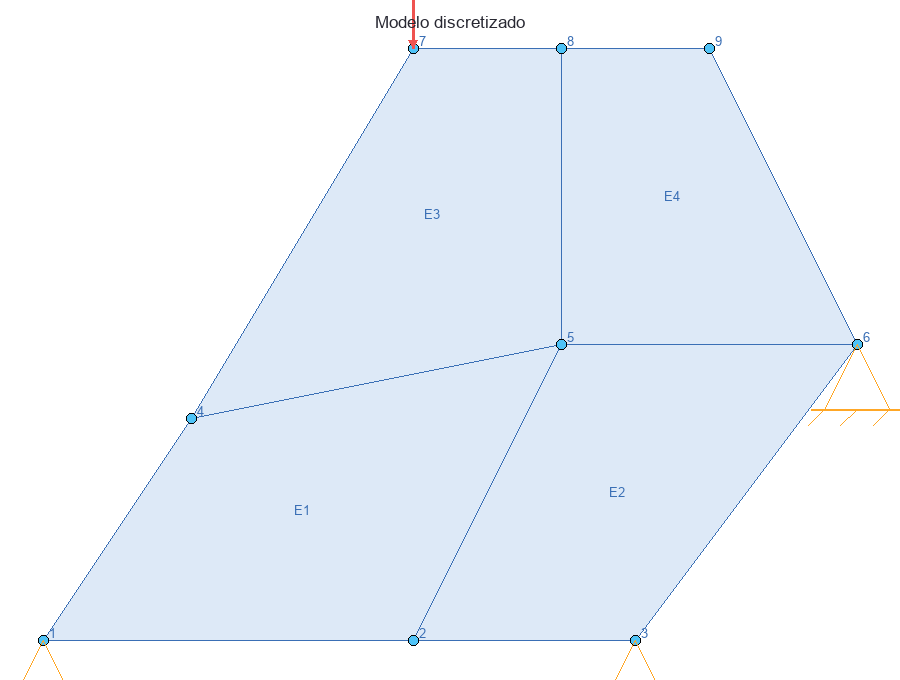
\includegraphics[width=0.74\linewidth]{mem_modelo}
\caption[Modelo discretizado del ejemplo guía.]{Modelo discretizado: malla, carga puntual $P=\valP$ aplicada hacia abajo en el nodo 7 y los dos desplazamientos restringidos en los nodos 1, 3 y 6.}
\label{fig:mem-modelo}
\end{figure}

\noindent
% El reparto es 0,34 / 0,62 y no mitad y mitad: la tabla de nodos son tres
% columnas de numeros (3,5 cm de ancho natural) y la de la derecha carga ademas
% el bloque de parametros globales, cuya fila mas larga -"Apoyos / Nodos 1, 3, 6
% (empotrados)"- pide 9,4 cm y antes se salia al margen derecho.
\begin{minipage}[t]{0.34\linewidth}
\centering
\captionof{table}{Nodos del ejemplo guía y sus coordenadas (en las unidades del anexo).}
\label{tab:mem-nodos}
\begin{tabular}{c r r}
\toprule
Nodo & $x$ & $y$ \\
\midrule
\nodosRows \\
\bottomrule
\end{tabular}
\end{minipage}
\hfill
\begin{minipage}[t]{0.62\linewidth}
\centering
\captionof{table}{Elementos (conectividad y espesor).}
\label{tab:mem-elem}
\begin{tabular}{c c c c c c}
\toprule
Elem. & $N_1$ & $N_2$ & $N_3$ & $N_4$ & $t$ \\
\midrule
\elementosRows \\
\bottomrule
\end{tabular}

\vspace{0.9em}
\captionof{table}{Parámetros globales del análisis.}
\label{tab:mem-param}
\begin{tabular}{@{}l l@{}}
\toprule
Parámetro & Valor \\
\midrule
Módulo de elasticidad & $E = \valE$ \\
Coeficiente de Poisson & $\nu = \valNu$ \\
Espesor & $t = \valT$ \\
Análisis & Tensión plana \\
Carga & $F_y = -\valP$ (nodo 7) \\
Apoyos & Nodos 1, 3, 6 ($u_x = u_y = 0$) \\
\bottomrule
\end{tabular}
\end{minipage}

\section{Procedimiento}

\subsection{Matriz constitutiva}

La matriz constitutiva de tensión plana es la de la \autoref{eq:D-tension-plana}. Con $E=\valE$ y $\nu=\valNu$ resulta, idéntica para los cuatro elementos, que comparten material:
% Partida en dos renglones: las tres matrices 3x3 seguidas mas la fraccion no
% entran en el ancho de linea y se metian 0,9 cm en el margen derecho.
\begin{align*}
\bm{D}&=\frac{E}{1-\nu^{2}}
\begin{bmatrix} 1 & \nu & 0 \\ \nu & 1 & 0 \\ 0 & 0 & \tfrac{1-\nu}{2} \end{bmatrix}
=\valDfactor\;\DmatNorm \\[0.4em]
&=\Dmat .
\end{align*}

\subsection{Rigidez del elemento}

Se desarrolla el elemento E\showId{} (nodos \showNodes); los tres restantes se calculan igual. Es el de mayor energía de deformación una vez resuelto el modelo, $U_e=\tfrac12\,\bm{u}_e^{T}\bm{k}_e\,\bm{u}_e$ (\energiaInline), el mismo criterio con que la memoria elige el elemento que desarrolla en las mallas mayores (\autoref{sec:memoria-io}). Sus coordenadas nodales son
\[
\bm{X}_e=\Xemat .
\]
En el punto de Gauss $\gpA$, las derivadas de las funciones de forma de la \autoref{eq:N-q4} en coordenadas naturales valen
\[
\partial\bm{N}_{\xi\eta}=\dNnatA .
\]
El Jacobiano de la \autoref{eq:jacobiano}, su determinante (\autoref{eq:detJ}) y su inversa por cofactores (\autoref{eq:invJ}) son
% Idem: las tres igualdades en un renglon se pasaban del margen.
\begin{align*}
\bm{J}&=\partial\bm{N}_{\xi\eta}\,\bm{X}_e=\Jmata, \qquad
\det\bm{J}=\detJa, \\[0.4em]
\bm{J}^{-1}&=\invJa,
\end{align*}
y las derivadas físicas, obtenidas por la regla de la cadena de la \autoref{eq:fisica-natural}, y la matriz $\bm{B}$ de la \autoref{eq:matriz-B} ($3\times 8$, que ordena esas derivadas según $\bm{\varepsilon}=\bm{B}\,\bm{u}_e$) resultan
\[
\partial\bm{N}_{xy}=\bm{J}^{-1}\,\partial\bm{N}_{\xi\eta}=\dNphysA ,
\]
{\footnotesize\setlength{\arraycolsep}{4pt}
\[
\bm{B}=\Bmata .
\]
}%
La rigidez del elemento es la cuadratura de la \autoref{eq:ke-gauss} sobre los cuatro puntos de Gauss (pesos $w_g=1$; determinantes $\det\bm{J}_g \in \{\detJinline\}$):
\[
\bm{k}_e=\sum_{g=1}^{4} w_g\,\bm{B}_g^{T}\,\bm{D}\,\bm{B}_g\,\lvert\det\bm{J}_g\rvert\,t .
\]
{\footnotesize\setlength{\arraycolsep}{3.5pt}
\[
\bm{k}_e=\keScale\cdot\keMat .
\]
}%

\subsection{Ensamblaje}

Cada $\bm{k}_e$ se dispersa a la matriz global según los grados de libertad (GDL) de sus nodos, con el operador de ensamblaje de la \autoref{eq:ensamblaje}; las cargas nodales arman $\bm{F}$:
\[
\bm{K}=\Ensamblaje_{e=1}^{4}\bm{k}_e \quad(\nDof\times\nDof),
\qquad
\bm{F}:\; F_{(7,y)}=-\valP,\ \text{resto } 0 .
\]
Como los identificadores del ejemplo son contiguos (1 a 9), el nodo $n$ recibe el ordinal $i = n-1$ y sus dos GDL ocupan las posiciones $2i$ y $2i+1$ del sistema (\autoref{sec:identidad-gdl}); contadas desde uno, como en este anexo, son la $2n-1$ y la $2n$. Así, los nodos 4, 5, 8 y 7 de E\showId{} ocupan los GDL globales 7-8, 9-10, 15-16 y 13-14, y cada término de $\bm{k}_e$ se suma en la posición de $\bm{K}$ que indican esos índices. La \autoref{fig:mem-K} muestra el patrón de entradas no nulas de $\bm{K}$.

\begin{figure}[H]
\centering
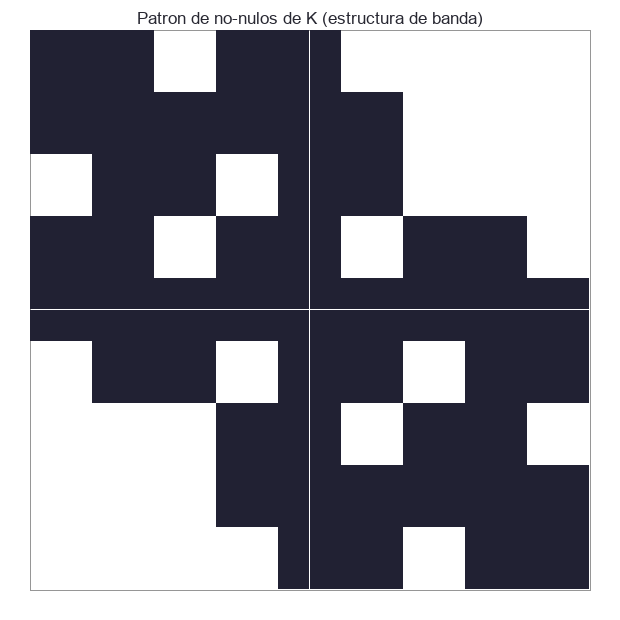
\includegraphics[width=0.42\linewidth]{mem_Ksparsity}
\caption[Patrón de entradas no nulas de la matriz de rigidez global.]{Patrón de entradas no nulas de la matriz de rigidez global $\bm{K}$ ($\nDof\times\nDof$). Cada bloque $2\times 2$ acopla dos nodos vecinos; el nodo central 5, compartido por los cuatro elementos, concentra el mayor número de acoplamientos.}
\label{fig:mem-K}
\end{figure}

\subsection{Restricciones y solución}

Los nodos 1, 3 y 6 fijan sus dos GDL (posiciones 1-2, 5-6 y 11-12 de $\bm{K}$, contadas desde uno): quedan \nRestr{} GDL restringidos y \nFree{} libres. Reordenando el sistema en bloques libre ($f$) y restringido ($r$), según la partición de la \autoref{eq:particion},
\[
\begin{bmatrix} \bm{K}_{ff} & \bm{K}_{fr} \\ \bm{K}_{rf} & \bm{K}_{rr} \end{bmatrix}
\begin{bmatrix} \bm{u}_{f} \\ \bm{u}_{r} \end{bmatrix}
=\begin{bmatrix} \bm{F}_{f} \\ \bm{F}_{r} \end{bmatrix},
\]
con $\bm{u}_r=\bm{0}$ el subsistema libre ($\nFree\times\nFree$) se reduce a
\[
\bm{K}_{ff}\,\bm{u}_{f}=\bm{F}_{f},
\qquad
\bm{F}_{f}^{T}=\bigl[\,0\ \cdots\ -\valP\ \cdots\ 0\,\bigr] .
\]
El motor resuelve este subsistema por factorización LU dispersa, con el reordenamiento de mínimo grado de la \autoref{sec:motor}, y entrega los desplazamientos nodales de la \autoref{tab:mem-resultados}; la comprobación del paso es el equilibrio de las reacciones que sigue.

\subsection{Reacciones}

En los GDL restringidos, $\bm{R}=\bm{K}\,\bm{u}-\bm{F}$ (\autoref{tab:mem-reacciones}):
\begin{center}
\captionof{table}{Reacciones en los nodos restringidos y su resultante.}
\label{tab:mem-reacciones}
\begin{tabular}{c r r}
\toprule
Nodo & $R_x$ & $R_y$ \\
\midrule
\reaccRows \\
\midrule
$\sum$ & $\RxTot$ & $\RyTot$ \\
\bottomrule
\end{tabular}
\end{center}
La resultante vertical, $\RyTot$, equilibra la carga aplicada, $-\valP$, dentro de la precisión con que se imprimen los valores, y la horizontal es nula. Que las dos sumas cierren se sigue por construcción de $\bm{R}=\bm{K}\,\bm{u}-\bm{F}$, porque una traslación rígida no produce fuerzas; la comprobación no mide exactitud, pero delataría un error de ensamblaje o un sistema mal resuelto.

\subsection{Recuperación de tensiones}

En cada punto de Gauss del elemento, $\bm{\varepsilon}=\bm{B}\,\bm{u}_e$ (forma matricial de la \autoref{eq:cinematica}) y $\bm{\sigma}=\bm{D}\,\bm{\varepsilon}$, con los desplazamientos de la \autoref{tab:mem-resultados} ordenados según la conectividad de E\showId{} (nodos \showNodes):
\[
\begin{aligned}
\bm{u}_e^{T}=\bigl[\,&{-}3{,}851\times10^{-4},\ -4{,}272\times10^{-3},\ -1{,}078\times10^{-3},\ -4{,}374\times10^{-3},\\
&{-}5{,}398\times10^{-3},\ -5{,}605\times10^{-3},\ -6{,}894\times10^{-3},\ -1{,}308\times10^{-2}\,\bigr].
\end{aligned}
\]
Los valores se imprimen redondeados ---las tensiones del primer punto de Gauss y las principales llevan un decimal más que las de las tablas---: rehacer $\bm{B}\,\bm{u}_e$ con las cifras impresas reproduce $\bm{\varepsilon}$ con tres cifras significativas. En $\gpA$:
\[
\bm{\varepsilon}=\epsA,
\qquad
\bm{\sigma}=\sigA .
\]
Las tensiones principales y la de von Mises de la \autoref{eq:principales-vm}, en su forma plana ($\sigma_z = 0$ en tensión plana), resultan en ese punto
\[
\sigma_{1,2}=\frac{\sigma_x+\sigma_y}{2}\pm\sqrt{\Bigl(\tfrac{\sigma_x-\sigma_y}{2}\Bigr)^{2}+\tau_{xy}^{2}}=\savgA\pm\radiusA=\sigOneA;\ \sigTwoA ,
\]
\[
\sigma_{\mathrm{VM}}=\sqrt{\sigma_1^{2}-\sigma_1\sigma_2+\sigma_2^{2}}=\vmA .
\]
Repetida la operación en los cuatro puntos de Gauss —numerados $(-,-)$, $(-,+)$, $(+,-)$, $(+,+)$—, cada componente cartesiana se lleva a los nodos mediante la matriz de extrapolación constante $\bm{E}=\bm{M}^{-1}$ de la \autoref{eq:extrap-q4}, $\bm{\sigma}_{\mathrm{nod}}=\bm{E}\,\bm{\sigma}_{\mathrm{PG}}$; por ejemplo, para $\sigma_x$ (nodos \showNodes):
{\footnotesize\setlength{\arraycolsep}{4pt}
\[
\sigxNodal=\Eextrap\,\sigxGauss .
\]
}%
En negrita, $\bm{E}$ es esa matriz de extrapolación, que no debe confundirse con el módulo de elasticidad $E=\valE$ ni con los rótulos E1 a E4 de los elementos.
Las Tablas \ref{tab:mem-gauss} y \ref{tab:mem-extrap} reúnen las tres componentes cartesianas y la tensión de von Mises, en los puntos de Gauss y en los nodos del elemento E\showId{}. La extrapolación se aplica únicamente a las componentes cartesianas: la tensión de von Mises de cada nodo se recalcula con la \autoref{eq:principales-vm} a partir de las componentes ya extrapoladas, por ser una función no lineal de ellas (\autoref{sec:resolucion-tensiones}).

\noindent
\begin{minipage}[t]{0.49\linewidth}
\centering
\captionof{table}{Tensiones en los puntos de Gauss (E\showId).}
\label{tab:mem-gauss}
\footnotesize
\begin{tabular}{c r r r r}
\toprule
PG & $\sigma_x$ & $\sigma_y$ & $\tau_{xy}$ & $\sigma_{\mathrm{VM}}$ \\
\midrule
\gaussStressRows \\
\bottomrule
\end{tabular}
\end{minipage}
\hfill
\begin{minipage}[t]{0.49\linewidth}
\centering
\captionof{table}[Tensiones extrapoladas a los nodos de E\showId.]{Tensiones extrapoladas a los nodos de E\showId, en el orden de su conectividad, que es el de las filas de $\bm{E}$.}
\label{tab:mem-extrap}
\footnotesize
\begin{tabular}{c r r r r}
\toprule
Nodo & $\sigma_x$ & $\sigma_y$ & $\tau_{xy}$ & $\sigma_{\mathrm{VM}}$ \\
\midrule
\nodalStressShowRows \\
\bottomrule
\end{tabular}
\end{minipage}

\medskip
\noindent El campo nodal final (\autoref{tab:mem-resultados}) promedia, en cada nodo, las contribuciones de los elementos que lo comparten. Como en la extrapolación, el promedio recae solo sobre las componentes cartesianas, y así cada fila de la tabla es coherente consigo misma.

\section{Resultados}

La \autoref{tab:mem-resultados} reúne, por nodo, los desplazamientos (solución del sistema) y las tensiones recuperadas y promediadas entre los elementos que comparten cada nodo.

\begin{table}[H]
\centering
\caption{Resultados nodales: desplazamientos y tensiones promediadas, en las unidades del anexo.}
\label{tab:mem-resultados}
\setlength{\tabcolsep}{5pt}
\begin{tabular}{c r r r r r r}
\toprule
Nodo & $u_x$ & $u_y$ & $\sigma_x$ & $\sigma_y$ & $\tau_{xy}$ & $\sigma_{\mathrm{VM}}$ \\
\midrule
\nodalAllRows \\
\bottomrule
\end{tabular}
\end{table}

\noindent El desplazamiento máximo es $\lvert\bm{u}\rvert_{\max}=\umaxMag$ en el nodo \umaxNode{} (donde se aplica la carga), y la tensión de von Mises máxima, $\sigma_{\mathrm{VM},\max}=\vmMax$ en el mismo nodo. Las cuatro energías elementales suman $6{,}54$, lo mismo que el trabajo de la carga, $\tfrac12\,P\,\lvert u_{7y}\rvert=\tfrac12\cdot\valP\cdot 1{,}308\times10^{-2}=6{,}54$. Como el equilibrio de las reacciones, ese balance se sigue de $\bm{K}\,\bm{u}=\bm{F}$, pero cruza las rigideces elementales con la solución global. Las Figuras \ref{fig:mem-deformada} y \ref{fig:mem-contorno} muestran la configuración deformada y el contorno de von Mises sobre la malla deformada, tal como los presenta el post-proceso del software.

% Dos figuras lado a lado SIN entorno figure: con \floatstyle{plaintop} un
% float con dos \caption conservaba solo el ultimo rotulo (la G.3 quedaba sin
% rotulo y el de la G.4 caia sobre la imagen equivocada). \captionof numera y
% ancla cada una por separado; el rotulo va arriba, como pide APA.
\medskip
\noindent
\begin{minipage}[t]{0.49\linewidth}
  \centering
  \captionof{figure}{Configuración deformada, amplificada $\times 84{,}1$, sobre la malla original.}
  \label{fig:mem-deformada}
  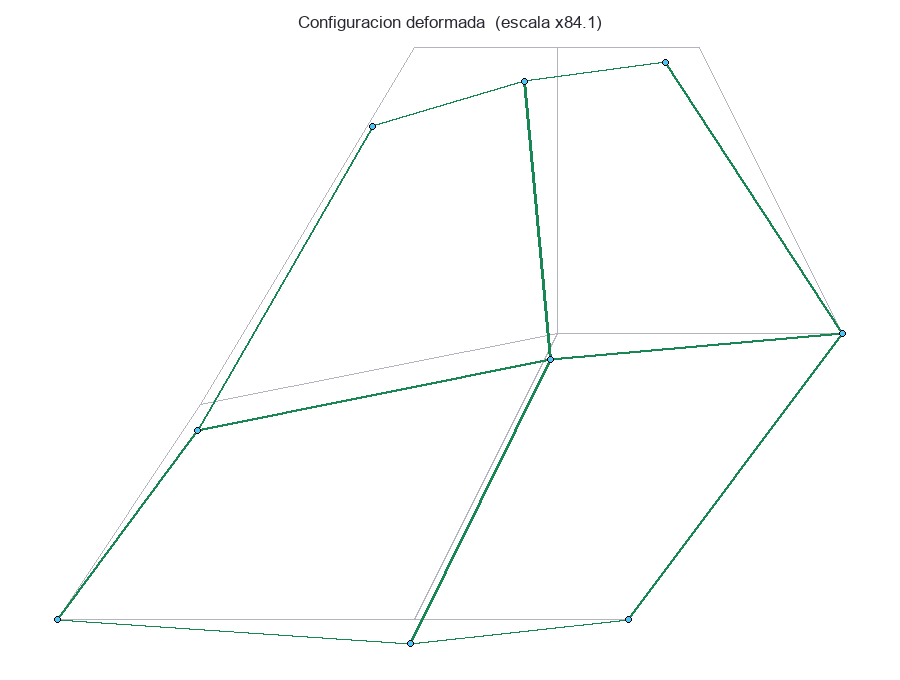
\includegraphics[width=\linewidth]{mem_deformada}
\end{minipage}
\hfill
\begin{minipage}[t]{0.49\linewidth}
  \centering
  \captionof{figure}[Contorno de von Mises sobre la malla deformada.]{Contorno de tensión de von Mises sobre la malla deformada; la escala va de $42{,}47$ a $864{,}70$, los extremos de la \autoref{tab:mem-resultados}.}
  \label{fig:mem-contorno}
  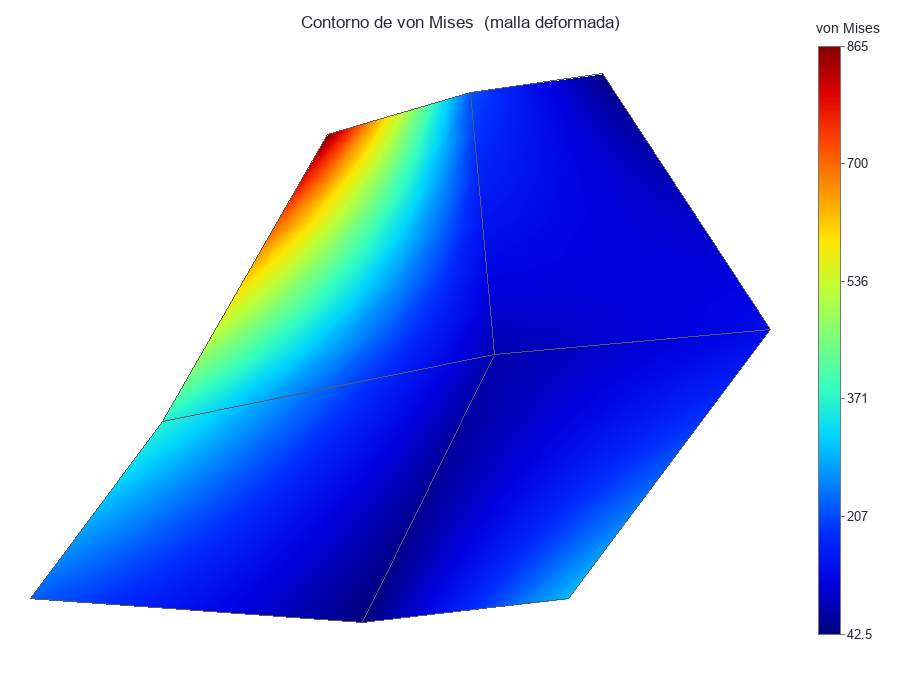
\includegraphics[width=\linewidth]{mem_contorno_vm}
\end{minipage}


\end{document}
